\documentclass[a5paper, openright, twoside, 12pt]{book}
\usepackage[main=polish, russian]{babel}
\usepackage{fontsetup}
\usepackage{graphicx}
\usepackage[
  top=10mm, headsep=3mm, headheight=15pt,
  bottom=13mm, footnotesep=3mm,
  left=8mm, right=8mm, bindingoffset=6mm]{geometry}
\usepackage{hyperref}
\usepackage{gchords}
\usepackage{array}
\usepackage{longtable}
\usepackage{multicol}
\usepackage{float}
\usepackage{xcolor}
\usepackage{fancyhdr}

%%%%%%%%%%%%%%%%%%%%

\makeatletter

\renewcommand*{\maketitle}{
  \begin{titlepage}
    \begin{center}
      \vspace*{3cm}
      \Huge \textsc{\@title}

      \vspace{0.3cm}
      \Large{\@author}

      \vspace{1cm}
      \fboxsep=1.5mm
      \fboxrule=1.5mm
      \fcolorbox{black}{black!70!}{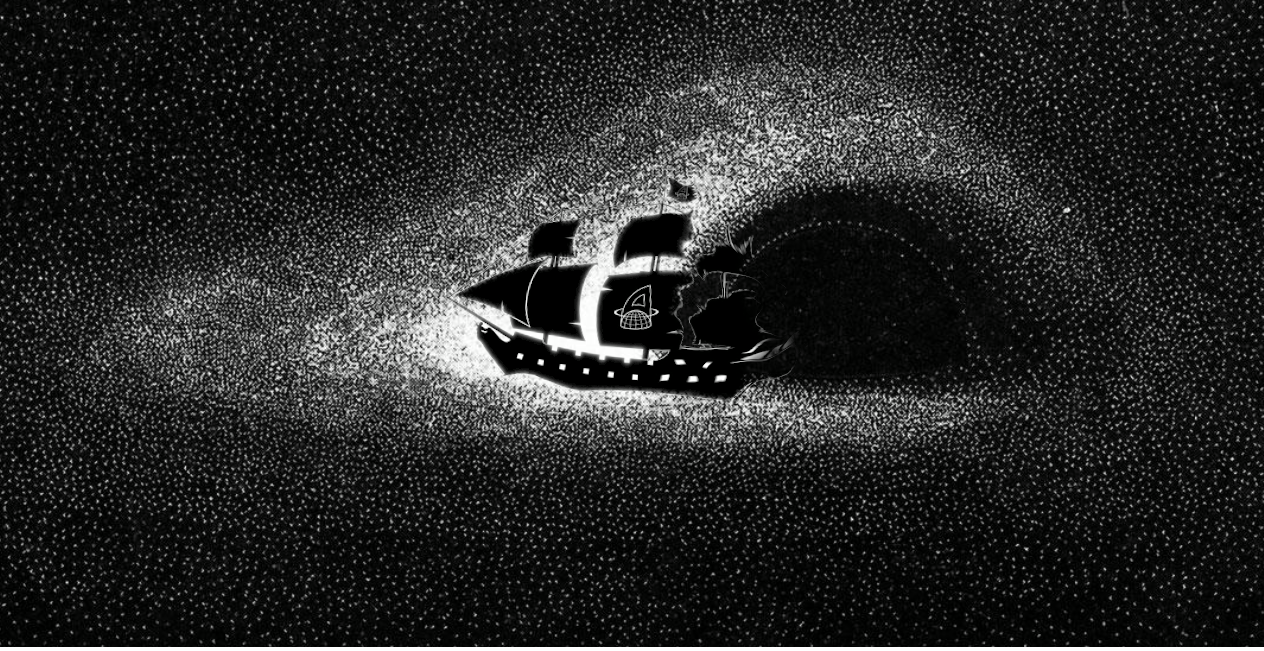
\includegraphics[width=10cm]{statek2.png}}

      \vspace{3cm}
      \Large{\@date}
    \end{center}
  \end{titlepage}
}

\renewcommand*{\tableofcontents}{
   \chapter* {\contentsname}
   \thispagestyle{fancy}
   \@starttoc{toc}
}

\renewcommand*{\section}{
  \@startsection{section}{1}{\z@}
    {-3.5ex \@plus -1ex \@minus -.2ex}
    {2ex \@plus .2ex}
    {\normalfont\large\bfseries}
}

\makeatother

%%%%%%%%%%%%%%%%%%%%

\author{stworzyły żagle}
\title{\uppercase{Pato}śpiewnik}
\date{ver. test}

\fancyhf{}
\fancyhead[RO]{\hyperref[toc]{\partcontent}}
\fancyhead[LE]{\uppercase{Pato} test}
\fancyfoot[C]{\thepage}
\renewcommand*{\headrulewidth}{0.5pt}
\renewcommand*{\footrulewidth}{0.5pt}

\setcounter{secnumdepth}{-2}

\newcommand*{\partcontent}{}
\newcommand*{\songssection}[2]{
  % #1 part title
  % #2 part subtitle
  \part[#1]{#1\\[10mm] {\normalfont{\Large #2}}}
  \renewcommand*{\partcontent}{#1}
}

\newcommand*{\refrenspace}{\hspace{5mm}}
\newcommand*{\akordy}[1]{{\bfseries #1}}

\newlength{\basezwrotkaspace}
\basezwrotkaspace=2mm
\newskip{\zwrotkaspace}
\zwrotkaspace=\basezwrotkaspace

\setlength{\LTpre}{0pt}
\setlength{\LTpost}{0pt}

\newenvironment*{piosenka}[2][8mm]
{ \section{#2} \begin{tabular}{@{}l@{\hspace{#1}}>{\bfseries}l} }
{ \end{tabular} }

\newenvironment*{piosenka_dluga}[2][8mm]
{ \section{#2} \begin{longtable}[l]{@{}l@{\hspace{#1}}>{\bfseries}l} }
{ \end{longtable} }

%%%%%%%%%%%%%%%%%%%%

\begin{document}

\pagestyle{empty}
\maketitle
\cleardoublepage

\pagestyle{fancy}
\tableofcontents
\label{toc}
\cleardoublepage

\songssection{Szanty}{Korycki, Żukowska, Porębski, Mechanicy Szanty\\ EKT Gdynia, Atlantyda, Ryczące Dwudzieski}
\newpage\begin{piosenka_dluga}{Alfabet bosmański -- Stare Dzwony}
A -- jak Atlantyk, co trzeba go przejść, & a G a \\*
B -- jak burta, a burty są dwie, & a F E \\*
C -- jak cuma -- ,,Hej, wybierz i obłóż ją!'' & a G \\*
D -- jak dryfkotwa i dirki i dno. & a G \\[\zwrotkaspace]

\refrenspace Hey derry, hay derry, hey derry down! & a F \\*
\refrenspace Masz kłopot -- weź łyka -- i kłopot już znika, & C G \\*
\refrenspace Po rumie, w tym szumie, nie może być źle! & a F \\*
\refrenspace Po rumie każdemu na morze się chce & C G \\[\zwrotkaspace]

E -- jak Eol, co sprzyja dziś nam, & a G a \\*
F -- jak fały -- ,,Hej, wybierać fał!'' & a F E \\*
G -- jak gejtawy, gordingi i grot, & a G \\*
H -- jest jak handszpak -- trza mocno pchać go. & a G \\[\zwrotkaspace]

%\refrenspace Hey derry, hay derry\ldots \\[\zwrotkaspace]

I -- to sygnał: ,,W lewo zmieniam mój kurs.'' & a G a \\*
J -- jak juzing -- trzeba żagle szyć znów, & a F E \\*
K -- jak kubryk, skąd leci nasz śpiew, & a G \\*
L -- jak latarnia, co błyski nam śle. & a G \\[\zwrotkaspace]

%\refrenspace Hey derry, hay derry\ldots \\[\zwrotkaspace]

Ł -- jak łańcuch -- ,,Hej, wybieraj go!'' & a G a \\*
M -- jak marsel, poniżej jest grot, & a F E \\*
N -- jak naktuz i nagiel, i nok, & a G \\*
O -- jak obijacz -- ,,Za burtę więc go!'' & a G \\[\zwrotkaspace]

%\refrenspace Hey derry, hay derry\ldots \\[\zwrotkaspace]

P -- jak pompy -- już znamy ten ruch, & a G a \\*
Q -- oznacza: ,,Mój statek jest zdrów.'' & a F E \\*
R -- jak reje, gdzie łazimy co dzień, & a G \\*
S -- tak jak stenga i saling, i ster. & a G \\[\zwrotkaspace]

%\refrenspace Hey derry, hay derry\ldots \\[\zwrotkaspace]

T -- jak trapy, co wiodą na ląd, & a G a \\*
U -- jak Uznam, gdzie znam każdy kąt, & a F E \\*
W -- jak wimpel -- prostuje go wiatr, & a G \\*
Z -- tak jak zejman, co płynie przez świat. & a G \\[\zwrotkaspace]

%\refrenspace Hey derry, hay derry\ldots \\[\zwrotkaspace]
\end{piosenka_dluga}
\newpage\begin{piosenka}{Biała sukienka -- Roman Roczeń}
Czasami, gdy mam chandrę i jestem sam & a e F C \\
Kieruję wzrok za okno, wysoko tam & a e F G C \\
Gdzie nad dachami domów i w noc, i dniem & E a D$^7$ G \\
Nadpływa kołysząca, marzeniem, snem & a e F G C \\[\zwrotkaspace]

\refrenspace I ona taka w tej białej sukience & C G \\
\refrenspace Jak piękny ptak, który zapiera w piersi dech & C F C \\
\refrenspace Chwyciłem mocno jej obie ręce & G C F \\
\refrenspace Oczarowany, zasłuchany w słodki śmiech & C D$^7$ G G$^7$ \\[\zwrotkaspace]

\refrenspace I cała w żaglach, jak w białej sukience & C G \\
\refrenspace Jak piękny ptak, który zapiera w piersi dech & C F C \\
\refrenspace Chwyciłem mocno ster w obie ręce & G C F \\
\refrenspace I żeglowałem zasłuchany w fali śpiew & C G C \\[\zwrotkaspace]

Wspomnienia przemijają, a w sercu żal & a e F C \\
Wciąż w łajbę się przemienia dziewczęcy czar & a e F G C \\
Jeżeli mi nie wierzysz, to gnaj co tchu & E a D$^7$ G \\
Tam z kei możesz ujrzeć coś z mego snu & a e F G C \\[\zwrotkaspace]

\refrenspace I ona taka w tej białej sukience\ldots \\[\zwrotkaspace]

Nie wiem, czy jeszcze kiedyś zobaczę ją & a e F C \\
Czy tylko w moich myślach jej oczy lśnią & a e F G C \\
Gdy pochylona, ostro do wiatru szła & E a D$^7$ G \\
Znowu się przeplatają obrazy dwa & a e F G C \\[\zwrotkaspace]

\refrenspace I ona taka w tej białej sukience\ldots \\
\end{piosenka}

\newpage\begin{piosenka}[3mm]{Bitwa -- Mechanicy Shanty}

Okręt nasz wpłynął w mgłę i fregaty dwie & a G F d \\
Popłynęły naszym kursem, by nie zgubić się & a G C E \\
Potem szkwał wypchnął nas poza mleczny pas & a G F d \\
I nikt wtedy nie przypuszczał, że fregaty śmierć nam niosą & a G C E \\[\zwrotkaspace]

\refrenspace Ciepła krew poleje się strugami & C G a e \\
\refrenspace Wygra ten, kto utrzyma ship & F G a \\
\refrenspace W huku dział ktoś przykryje się falami & C G a e \\
\refrenspace Jak da Bóg, ocalimy bryg & F G a \\[\zwrotkaspace]

Nagły huk w uszach grał i już atak trwał & a G F d \\
To fregaty uzbrojone rzędem w setkę dział & a G C E \\
Czarny dym spowił nas, przyszedł śmierci czas & a G F d \\
Krzyk i lament mych kamratów, przerywany ogniem katów & a G C E \\[\zwrotkaspace]

\refrenspace Ciepła krew\ldots \\[\zwrotkaspace]

Pocisk nasz trafił w maszt, usłyszałem trzask & a G F d \\
To sterburtę rozwaliła jedna z naszych salw & a G C E \\
,,Żagiel staw'', krzyknął ktoś, znów piratów złość & a G F d \\
Bo od rufy nam powiało, a fregatom w mordę wiało & a G C E \\[\zwrotkaspace]

\refrenspace Ciepła krew\ldots \\[\zwrotkaspace]

Z fregat dwóch tylko ta pierwsza w pogoń szła & a G F d \\
Wnet abordaż rozpoczęli, gdy dopadli nas & a G C E \\
Szyper ich dziury dwie zrobił w swoim dnie & a G F d \\
Nie pomogło to psubratom, reszta z rei zwisa za to & a G C E \\[\zwrotkaspace]

\refrenspace Ciepła krew\ldots \\[\zwrotkaspace]

Po dziś dzień tamtą mgłę i fregaty dwie & a G F d \\
Kiedy noc zamyka oczy, widzę w moim śnie & a G C E \\
Tamci, co śpią na dnie, uśmiechają się & a G F d \\
Że ich straszną śmierć pomścili bracia, którzy zwyciężyli & a G C E \\[\zwrotkaspace]

\refrenspace Ciepła krew\ldots \\

\end{piosenka}
\newpage\begin{piosenka}{Bramy Dublina -- Mechanicy Shanty}

Chciałbym ptakiem być -- pewien starzec mi rzekł -- & a F C G \\
I polecieć daleko tam, & a e \\
Gdzie przed laty stał rodzinny mój dom, & a F C G \\
Gdym opuszczał me Dublin Town. & a e a \\[\zwrotkaspace]

Młody byłem tak, pełen wiary, że świat & a F C G \\
Czeka na to, by odkryć go. & a e \\
Opuściłem dom, porwał mnie życia prąd, & a F C G \\
Związał z morzem historię mą. & a e a \\[\zwrotkaspace]

\refrenspace Ten stary port, wąskich ulic gwar, & C G \\
\refrenspace Wciąż wspominam jak starą pieśń, & a e \\
\refrenspace Która niesie mnie poprzez noce i dnie & a F C G \\
\refrenspace Do otwartych Dublina bram. & a e a \\[\zwrotkaspace]

W małym porcie, gdzie zacumował nasz ship, & a F C G \\
Zobaczyłem ją z koszem róż. & a e \\
Włosy niby len rozczesywał jej wiatr, & a F C G \\
Błękit oczu roztopił lód. & a e a \\[\zwrotkaspace]

Chciałem poznać ją, rzucić świat jej do stóp, & a F C G \\
Lecz odwagi zabrakło mi. & a e \\
Dzisiaj wiem -- to błąd, trzeba szczęście swe brać, & a F C G \\
Kiedy stuka do Twoich drzwi. & a e a \\[\zwrotkaspace]

\refrenspace Ten stary port\ldots \\

\end{piosenka}

\newpage\begin{piosenka}{Branka -- Ryczące Dwudziestki}

W dół od rzeki, poprzez London Street, \\
Psów królewskich oddział zwarty szedł. \\
Ojczyźnie trzeba dziś świeżej krwi, \\
Marynarzy floty wojennej. \\[\zwrotkaspace]

A że byłem wtedy silny chłop, \\
W tłumie złowił mnie sierżanta wzrok. \\ 
W kajdanach z bramy wywlekli mnie, \\
Marynarza floty wojennej. \\[\zwrotkaspace]

Jak o prawa upominać się \\
Na gretingu nauczyli mnie. \\
Niejeden krwią wtedy spłynął grzbiet \\ 
Marynarza floty wojennej. \\[\zwrotkaspace]

Nikt nie zliczy, ile krwi i łez \\
Wsiąkło w pokład, gdy się zaczął rejs, \\ 
Dla chwały twej, słodki kraju mój, \\
Marynarzy floty wojennej. \\[\zwrotkaspace]

Hen za rufą miły został dom, \\
Jesteś tylko parą silnych rąk. \\
Dowódca tu twoim bogiem jest, \\
Marynarzu floty wojennej. \\[\zwrotkaspace]

Gdy łapaczy szyk formuje się, \\
W pierwszym rzędzie możesz ujrzeć mnie. \\ 
Kto stanie na mojej drodze dziś, \\
Łup stanowi floty wojennej. \\[\zwrotkaspace]

\end{piosenka}
\newpage\begin{piosenka}{Chciałem być żeglarzem -- Andrzej Korycki}

Chciałem być żeglarzem, ale wziął mnie strach, & C G F C \\
Że mój okręt zginie gdzieś w dalekich mgłach. & C G F C \\
Bałem się, że człowiek w morzu może zgnić & C E a \\
I że rum ochrzczony będę musiał pić. & C G F C \\
\refrenspace Bałem się, że człowiek w morzu może zgnić & C E a \\
\refrenspace I że rum ochrzczony będę musiał pić. & C G F C \\[\zwrotkaspace]

\akordy{C G}\\[\zwrotkaspace]

Chciałem być żeglarzem, ale wziął mnie strach, & C G F C \\
Bo jak tu zostawić tych dziewcząt sto we łzach, & C G F C \\
No i w każdym porcie innych dziewczyn sto & C E a \\
Nie chcę być żeglarzem, bo męczące to. & C G F C \\
\refrenspace No i w każdym porcie innych dziewczyn sto & C E a \\
\refrenspace Nie chcę być żeglarzem, bo nieludzkie to. & C G F C \\[\zwrotkaspace]

\akordy{D A}\\[\zwrotkaspace]

Chciałem być żeglarzem, los inaczej chciał & D A G D \\
I zamiast sztormiaka gitarę mi dał. & D A G D \\
Widać w naszych kartach tak już musi stać, & D Fis h \\
Jedni mają pływać, inni mają grać. & D A G D \\
\refrenspace Widać w naszych kartach tak już musi stać, & D Fis h \\
\refrenspace Jedni mają pływać, inni mają grać. & D A G D \\[\zwrotkaspace]

Że wy macie pływać, a my dla was grać. & D A G D \\

\end{piosenka}

\newpage\begin{piosenka_dluga}{Cztery piwka -- Jerzy Porębski}

Ze Świnoujścia do Walvis Bay & d \\*
Droga nie była krótka, & d \\*
A po dwóch dobach, albo mniej, & d \\*  
Już się skończyła wódka. & d \\*
,,Do brydża!'' -- krzyknął Siwy Flaka & d \\*
I z miejsca rzekł -- ,,Dwa piki'', & d \\*
A ochmistrz w ,,telewizor'' wlał & d \\*
Nie byle jakie siki. & A$^7$ d \\[\zwrotkaspace]

\refrenspace Cztery piwka na stół, w popielniczkę pet, & D G \\*
\refrenspace Jakąś Damę roześmianą Król przytuli wnet. & A$^7$ D \\*
\refrenspace Gdzieś między palcami sennie płynie czas. & D$^7$ G \\*
\refrenspace ,,Czwarta ręka, Króla bije As!'' & A$^7$ d \\[\zwrotkaspace]

A w karcie tylko jeden As & d \\*
I nic poza tym nie ma, & d \\*
Ale nie powiem przecie -- ,,Pas'', & d \\*
Może zagrają szlema? & d \\*
,,Kontra'' -- mu rzekłem, taki bluff, & d \\*
By nieco spuścił z tonu, & d \\*
A Fred mu na to -- ,,Cztery trefl!'' & d \\*
Przywalił bez pardonu. & A$^7$ d \\[\zwrotkaspace]

\refrenspace Cztery piwka na stół\ldots \\[\zwrotkaspace]

A ,,mój'' w dwa palce obtarł nos, & d \\*
To znaczy: nie ma nic\ldots & d \\*
I wtedy Flak, podnosząc głos, & d \\*
Powiedział -- ,,Cztery pik!'' & d \\*
I kiedy jeszcze cztery Króle & d \\*
Pokazał mu jak trza, & d \\*
To Fred, z renonsem -- ,,Siedem pik'' -- & d \\*
Powiedział -- ,,Niech gra Flak!'' & A$^7$ d \\[\zwrotkaspace]

\refrenspace Cztery piwka na stół\ldots \\[\zwrotkaspace]

A ja mu -- ,,Kontra'', on mi -- ,,Re'', & d \\*
Ja czuję pełen luz, & d \\*
Bo widzę w moich kartach, że & d \\*
Jest atutowy tuz. & d \\*
Więc strzelam! Kiedy karty Fred & d \\*
Wyłożył mu na blat, & d \\*
To każdy mógł zobaczyć, jak & d \\*
Siwego Flaka trafia szlag. & A$^7$ d \\[\zwrotkaspace]

\refrenspace Cztery piwka na stół, w popielniczkę pet, & D G \\*
\refrenspace Jakąś Damę roześmianą Król przytuli wnet. & A$^7$ D \\*
\refrenspace Gdzieś między palcami sennie płynie czas. & D$^7$ G \\*
\refrenspace ,,Czwarta ręka, Króla bije As!'' & A$^7$ d \\[\zwrotkaspace]

Już nie pamiętam, ile dni & d \\*
W miesiące złożył czas. & d \\*
Morszczuki dosyć dobrze szły & d \\*
I grało się nie raz & d \\*
Lecz nigdy więcej Siwy Flak, & d \\*
Klnę na jumprowe wszy, & d \\*
Choćbyś go prosił tak, czy siak & d \\*
Nie zasiadł już do gry! & A$^7$ d \\[\zwrotkaspace]

\refrenspace W popielniczkę pet, cztery piwka na stół & D G \\*
\refrenspace Już tej Damy roześmianej nie przytuli Król & A$^7$ D \\*
\refrenspace Gdzieś nam się zapodział atutowy As, & D$^7$ G \\*
\refrenspace Tego Szlema z nami wygrał czas! & A$^7$ d \\[\zwrotkaspace]

\refrenspace Cztery piwka na stół, w popielniczkę pet, & D G \\*
\refrenspace Jakąś Damę roześmianą Król przytuli wnet. & A$^7$ D \\*
\refrenspace Gdzieś między palcami sennie płynie czas. & D$^7$ G \\*
\refrenspace ,,Czwarta ręka, Króla bije As!'' & A$^7$ d \\

\end{piosenka_dluga}
\newpage\begin{piosenka}{24 lutego -- EKT Gdynia}
To dwudziesty czwarty był lutego, & C \\
Poranna zrzedła mgła, & G \\
Wyszło z niej siedem uzbrojonych kryp, & a \\
turecki niosły znak. & a G a \\ [\zwrotkaspace]

\refrenspace No i znów bijatyka, & G C \\
\refrenspace I znów bijatyka, & G C \\
\refrenspace I bijatyka cały dzień, & G C G \\
\refrenspace I porąbany dzień, i porąbany łeb, & a G C \\
\refrenspace Razem bracia aż po zmierzch. & a G a \\ [\zwrotkaspace]


Już pierwszy skrada się do burt, & C \\
A zwie się Goździk Lee, & G \\
Z Algieru Pasza wysłał go, & a \\
Aby nam upuścić krwi. & a G a \\ [\zwrotkaspace]

\refrenspace No i znów bijatyka\ldots \\ [\zwrotkaspace]

To już drugi skrada się do burt, & C \\
A zwie się Róży Pąk, & G \\
Plunęliśmy ze wszystkich rur, & a \\
Bardzo szybko szedł na dno. & a G a \\ [\zwrotkaspace]

\refrenspace No i znów bijatyka\ldots \\ [\zwrotkaspace]

W naszych rękach dwa i dwa na dnie, & C \\
Cała reszta zwiała gdzieś, & G \\
A jeden z nich zabraliśmy, & a \\
Na starej Anglii brzeg. & a G a \\ [\zwrotkaspace]

\refrenspace No i znów bijatyka\ldots \\ 

\end{piosenka}
\newpage\begin{piosenka}{Dziesięć w skali Beauforta -- Trzy Korony}
Kołysał nas zachodni wiatr & a d \\
Brzeg gdzieś za rufą został & E$^7$ a \\
I nagle ktoś jak papier zbladł & d a \\
Sztorm idzie, panie bosman! & H$^7$ E$^7$ \\ [\zwrotkaspace]

\refrenspace A bosman tylko zapiął płaszcz & F C F C \\
\refrenspace I zaklął: ech, do czorta! & F E$^7$ a \\
\refrenspace Nie daję łajbie żadnych szans & F G a E$^7$ a \\
\refrenspace Dziesięć w skali Beauforta! & F E$^7$ a \\ [\zwrotkaspace]

Z zasłony ołowianych chmur & a d \\
Ulewa spadła nagle & E$^7$ a \\
Rzucało nami w górę, w dół & d a \\
I fala zmyła żagle & H$^7$ E$^7$ \\ [\zwrotkaspace]

\refrenspace A bosman\ldots \\ [\zwrotkaspace]

O pokład znów uderzył deszcz & a d \\
I padał już do rana & E$^7$ a \\
Piekielnie ciężki to był rejs & d a \\
Szczególnie dla bosmana & H$^7$ E$^7$ \\ [\zwrotkaspace]

\refrenspace A bosman tylko zapiął płaszcz & F C F C \\
\refrenspace I zaklął: ech, do czorta! & F E$^7$ a \\
\refrenspace Przedziwne czasem sny się ma & F G a E$^7$ a \\
\refrenspace Dziesięć w skali Beauforta! & F E$^7$ a \\
\refrenspace Dziesięć w skali Beauforta! & F E$^7$ a \\
\refrenspace Dziesięć w skali Beauforta! & F E$^7$ a \\
\end{piosenka}

\newpage\begin{piosenka_dluga}{Emeryt -- EKT Gdynia}

Leżysz wtulona w pościel, & d \\*
Coś cichutko mruczysz przez sen & a \\*
Łóżko szerokie a pościel świeża & F \\*
-- za oknem prawie dzień\ldots & A \\*
A jeszcze niedawno koja & d \\*
I jej pachnący rybą koc & C \\*
Fale bijące o pokład & F \\*
I bosmana zdarty głos & A \\[\zwrotkaspace]

\refrenspace To wszystko było, minęło & d \\*
\refrenspace -- zostało tylko wspomnienie\ldots & C G d \\*
\refrenspace Już nie poczuję wibracji pokładu, & d C \\*
\refrenspace Gdy kable grają\ldots & C G d \\*
\refrenspace Już tylko dom i ogródek i tak & d C \\*
\refrenspace Aż do śmierci. & C G d \\*
\refrenspace A przecież stare żaglowce & d \\*
\refrenspace Po morzach jeszcze pływają\ldots & C G d \\[\zwrotkaspace]

Nie gniewaj się kochanie, & d \\*
Że trudno ze mną żyć & a \\*
Że zapomniałem kupić mleko & F \\*
I gary zmyć\ldots & A \\*
Lecz jeszcze niedawno okręt & d \\*
Mym drugim domem był & C \\*
Tam nie stało się w kolejkach, & F \\*
Tam nie było miejsca dla złych & A \\[\zwrotkaspace]

\refrenspace To wszystko było\ldots \\[\zwrotkaspace]

Upłynie sporo czasu & d \\*
Nim przyzwyczaję się & a \\*
Czterdzieści lat na morzu, & F \\*
Zamkniętych w jeden dzień & A \\*
Skąd lekarz może wiedzieć, & d \\*
Że za morzem tęskno mi? & C \\*
Że duszę sie na lądzie, & F \\*
Że śni mi się pokład pełen ryb? & A \\[\zwrotkaspace]

\refrenspace To wszystko było, minęło & d \\*
\refrenspace -- zostało tylko wspomnienie\ldots & C G d \\*
\refrenspace Już nie poczuję wibracji pokładu, & d C \\*
\refrenspace Gdy kable grają\ldots & C G d \\*
\refrenspace Już tylko dom i ogródek i tak & d C \\*
\refrenspace Aż do śmierci. & C G d \\*
\refrenspace A przecież stare żaglowce & d \\*
\refrenspace Po morzach jeszcze pływają\ldots & C G d \\[\zwrotkaspace]

Wiem, że masz do mnie żal, & d \\*
Mieliśmy do przyjaciół iść & a \\*
Spotkałem kolegę z rejsu, & F \\*
On w morze idzie dziś\ldots & A \\*
Siedziałem potem na kei, & d \\*
Ze łzami patrzyłem w port & C \\*
Jeszcze przyjdzie dzień, & F \\*
Że opuszczę go\ldots A narazie\ldots & a \\[\zwrotkaspace]

\refrenspace To wszystko było\ldots \\[\zwrotkaspace]

\end{piosenka_dluga}
\newpage\begin{piosenka}[5mm]{Fale -- Andrzej Korycki}

Późną nocą, pustym brzegiem idzie z nami mgła, & G D e \\
Fale zaraz nas dostrzegą, spójrz, już pierwsza gna. & G D H \\
Chciała podbiec tu, ale podły los & e a \\
Nie pozwolił jej zbyt długo żyć & D H \\
I zielone, mokre serce już przestało bić. & G D H \\[\zwrotkaspace]

\refrenspace Przez nikogo nie wołane -- przypływają & G D \\
\refrenspace I u stóp niezrozumiane -- umierają. & a e \\
\refrenspace Jeśli ktoś zna mowę tych upartych, dziwnych fal, & G D \\
\refrenspace Niech pogada z nimi, bo mi ich naprawdę żal. & a e \\[\zwrotkaspace]

Fale, czemu się godzicie na tę dolę złą, & G D e \\
Czemu do nas przychodzicie porzucając dom? & G D H \\
Choć, być może, przez was z rejsu ktoś & e a \\
Pozdrowienia, jak gołębiem, śle. & D H \\
Tutaj nikt was nie rozumie, trafiłyście źle. & G D H \\[\zwrotkaspace]

Późną nocą, gdzieś na brzegu mówi do mnie mgła: & G D e \\
-- ,,Próżno chciałbyś je ostrzegać, spójrz, następna gna\ldots'' & G D H \\
Chciała podbiec tu, ale podły los & e a \\
Nie pozwolił jej zbyt długo żyć. & D H \\
Zielone drugie serce już przestało bić. & G D H \\

\end{piosenka}
\newpage\begin{piosenka}{Gdzie ta keja -- Jerzy Porębski}

Gdyby tak ktoś przyszedł i powiedział: & a \\
Stary, czy masz czas? & G a \\
Potrzebuje do załogi jakąś nową twarz & C G G$^7$ C \\
Amazonka, Wielka Rafa, oceany trzy & C C$^7$ F d \\
Rejs na całość, rok, dwa lata, to powiedziałbym: & a E E$^7$ a \\[\zwrotkaspace]

\refrenspace Gdzie ta keja, a przy niej ten jacht? & a E$^7$ a \\
\refrenspace Gdzie ta koja wymarzona w snach? & C G C \\
\refrenspace Gdzie te wszystkie sznurki od tych szmat? & g A$^7$ d A$^7$ d \\
\refrenspace Gdzie ta brama na szeroki świat? & a E$^7$ a \\[\zwrotkaspace]

\refrenspace Gdzie ta keja, a przy niej ten jacht? & a E$^7$ a \\
\refrenspace Gdzie ta koja wymarzona w snach? & C G C \\
\refrenspace W każdej chwili płynę w taki rejs & g A$^7$ d A$^7$ d \\
\refrenspace Tylko gdzie to jest, no gdzie to jest? & a E$^7$ a \\[\zwrotkaspace]

Gdzieś na dnie starej szafy leży ostry nóż & a G a \\
Stare dżinsy wystrzępione impregnuje kurz & C G G$^7$ C  \\
W kompasie igła zardzewiała, lecz kierunek znam & C C$^7$ F d \\
Biorę wór na plecy i przed siebie gnam & a E E$^7$ a \\[\zwrotkaspace]

\refrenspace Gdzie ta keja\ldots \\[\zwrotkaspace]

Przeszły lata zapyziałe, rzęsą zarósł staw & a G a \\
A na przystani czółno stało -- kolorowy paw & C G G$^7$ C  \\
Zaokrągliły się marzenia, wyjałowiał step & C C$^7$ F d \\
Dalej marzy o załodze ten samotny łeb & a E E$^7$ a \\[\zwrotkaspace]

\refrenspace Gdzie ta keja\ldots \\

\end{piosenka}
\newpage\begin{piosenka}{Gdzieś tam -- Jerzy Porębski}

Gdzieś tam, na krańcach Wielkiej Wody, & D cis Fis \\
Gdzieś tam, gdzie giną ludzkie drogi, & h C D$^7$ \\
Gdzieś tam, gdzie siedzi stary, siwy Bóg, & G fis \\
Jest dom naszych wszystkich dusz. & e A$^7$ D \\[\zwrotkaspace]

Gdzieś tam, w syntezie wszelkich Światów, & D cis Fis \\
Gdzieś tam, bez wiary, bez dogmatów, & h C D$^7$ \\
Wśród naturalnych praw, & G fis \\
Do załatwienia mam parę spraw. & e A$^7$ D \\[\zwrotkaspace]

\refrenspace Po pierwsze, po drugie, po trzecie, po czwarte\ldots & Fis h E$^7$ \\
\refrenspace I co to życie było warte? & E$^7$ A$^7$ \\[\zwrotkaspace]

Gdzieś tam, gdzie nieśmiertelne żyje, & D cis Fis \\
Gdzieś tam, gdzie źródło prawdy bije, & h C D$^7$ \\
Gdzie zło i dobro traci sens, & G fis \\
W ostatni popłynę rejs. & e A$^7$ D \\[\zwrotkaspace]

Gdzieś tam, na drugą stronę cienia, & D cis Fis \\
Gdzieś tam, gdzie duch materię zmienia, & h C D$^7$ \\
Przejmę ostatnią z wacht, & G fis \\
Do kei przytulę jacht. & e A$^7$ D \\[\zwrotkaspace]

Gdzieś tam, na krańcach Wielkiej Wody, & D cis Fis \\
Gdzieś tam, gdzie giną ludzkie drogi, & h C D$^7$ \\
Gdzieś tam, gdzie siedzi stary, siwy Bóg, & G fis \\
Jest dom naszych wszystkich dusz\ldots & e A$^7$ D \\[\zwrotkaspace]

\end{piosenka}
\newpage\begin{piosenka_dluga}{Hej, me Bałtyckie Morze}

Hej, me Bałtyckie Morze, & a E a (G) \\*
Wdzięczny Ci jestem bardzo, & C G C C$^7$ \\*
Toś Ty mnie wychowało, & d G \\*
Toś Ty mnie wychowało, & C d \\*
Szkołęś mi dało twardą. & a E a (E) \\[\zwrotkaspace]

Szkołęś mi dało twardą,  & a E a (G) \\*
Uczyłoś łodzią pływać, & C G C C$^7$ \\*
Żagle pięknie cerować, & d G \\*
Żagle pięknie cerować & C d \\*
Codziennie pokład zmywać. & a E a (E) \\[\zwrotkaspace]

Codziennie pokład zmywać & a E a (G) \\*
Od soli i od kurzy, & C G C C$^7$ \\*
Mosiądze wyglansować, & d G \\*
Mosiądze wyglansować, & C d \\*
W ciszy, czy w czasie burzy. & a E a (E) \\[\zwrotkaspace]

W ciszy, czy w czasie burzy, & a E a (G) \\*
Trzeba przy pracy śpiewać, & C G C C$^7$ \\*
Bo kiedy śpiewu nie ma, & d G \\*
Bo kiedy śpiewu nie ma, & C d \\*
Neptun się będzie gniewać. & a E a (E) \\[\zwrotkaspace]

Neptun się będzie gniewać & a E a (G) \\*
I klątwę brzydką rzuci, & C G C C$^7$ \\*
Wpakuje na mieliznę, & d G \\*
Wpakuje na mieliznę, & C d \\*
Albo nam łódź wywróci. & a E a (E) \\[\zwrotkaspace]

Albo nam łódź wywróci & a E a (G) \\*
I krzyknie - ,,Hej partacze! & C G C C$^7$ \\*
Nakarmię wami rybki, & d G \\*
Nakarmię wami rybki, & C d \\*
Nikt po was nie zapłacze!'' & a E a (E) \\[\zwrotkaspace]

Nikt po nas nie zapłacze, & a E a (G) \\*
Nikt nam nie dopomoże, & C G C C$^7$ \\*
Za wszystkie miłe rady, & d G \\*
Za wszystkie miłe rady, & C d \\*
Dziękuję Tobie Morze. & a E a (E) \\[\zwrotkaspace]

Hej, me Bałtyckie Morze, & a E a (G) \\*
Wdzięczny Ci jestem bardzo, & C G C C$^7$ \\*
Toś Ty mnie wychowało, & d G \\*
Toś Ty mnie wychowało, & C d \\*
Szkołęś mi dało twardą. & a E a (E) \\[\zwrotkaspace]

\end{piosenka_dluga}
\newpage\begin{piosenka}{Hiszpańskie dziewczyny -- Ryczące Dwudziestki}

Żegnajcie nam dziś, hiszpańskie dziewczyny & e C H$^7$ \\
Żegnajcie nam dziś, marzenia ze snów & e G D \\
Ku brzegom angielskim już ruszać nam pora & C D e \\
Lecz kiedyś na pewno wrócimy tu znów & C H$^7$ e \\[\zwrotkaspace]

\refrenspace I smak waszych ust, hiszpańskie dziewczyny & e C H$^7$ \\
\refrenspace W noc ciemną i złą nam będzie się śnił & e G D \\
\refrenspace Leniwie popłyną znów rejsu godziny & C D e \\
\refrenspace Wspomnienie ust waszych przysporzy nam sił & C H$^7$ e \\[\zwrotkaspace]

Niedługo ujrzymy znów w dali Cape Deadman & e C H$^7$ \\
I Głowę Baranią sterczącą wśród wzgórz & e G D \\
I statki stojące na redzie przed Plymouth & C D e \\
Klarować kotwicę najwyższy czas już & C H$^7$ e \\[\zwrotkaspace]

\refrenspace I smak waszych ust\ldots \\[\zwrotkaspace]

Niedługo już żagle na masztach rozkwitną & e C H$^7$ \\
Kurs szyper wyznaczy do Portland i Wight & e G D \\
I znów stara łajba potoczy się ciężko & C D e \\
Przez fale w kierunku na Beachy, Fairlight & C H$^7$ e \\[\zwrotkaspace]

\refrenspace I smak waszych ust\ldots \\[\zwrotkaspace]

Zabłysną nam bielą skał zęby pod Dover & e C H$^7$ \\
I znów noc w kubryku wśród legend i bajd & e G D \\
Powoli i znojnie tak płynie nam życie & C D e \\
Na wodach i w portach przy South Foreland Light & C H$^7$ e \\[\zwrotkaspace]

\refrenspace I smak waszych ust\ldots \\

\end{piosenka}
\newpage \begin{piosenka}{Przestrzenie liniowe}
Żegnajcie nam dziś, przestrzenie liniowe, & e C H$^7$ \\
Żegnajcie nam dziś, macierze ich baz & e G D \\
Ku całkom Riemanna już ruszać nam pora & C D e \\
Lecz do tych przestrzeni wrócimy nie raz & C H$^7$ e \\ [\zwrotkaspace]

\refrenspace I smak waszych baz przestrzenie liniowe  & e C H$^7$ \\
\refrenspace W noc ciemną i złą nam będzie się śnił & e G D \\
\refrenspace Leniwie popłyną granice punktowe & C D e \\
\refrenspace Wspomnienie ciał waszych przysporzy nam sił & C H$^7$ e \\ [\zwrotkaspace]

Niedługo ujrzymy szeregi funkcyjne & e C H$^7$ \\
ekstremów lokalnych w przedziale (a b) & e G D \\
Dowody twierdzenia w notatkach z wykładów & C D e \\
lecz znów na kolokwium nam wyjdzie to źle & C H$^7$ e \\ [\zwrotkaspace]

Niedługo poprawek wyniki rozkwitną & e C H$^7$ \\
i każdy się dowie czy w końcu to zdał & e G D \\
Bo na analizie niepewny jest człowiek & C D e \\
Co pływa myślami wśród rzutów i ciał & C H$^7$ e \\ [\zwrotkaspace]

Zabłysną nam bielą porządki liniowe & e C H$^7$ \\
I wykład upłynie wśród legend i bajd & e G D \\
moc klasy abstrakcji relacji zerowej & C D e \\
Po zbiorach niepustych zrobimy znów rajd & C H$^7$ e \\ [\zwrotkaspace]

Niedługo zbiór liczb naturalnych zabłyśnie & e C H$^7$ \\
Ciągami co nigdy nie zbiegną do zer & e G D \\
I moc continuum nad nami zawiśnie & C D e \\
Bijekcją nas rzuci rekinom na żer & C H$^7$ e \\ [\zwrotkaspace]

Zawiniem do portu przy sekcji studenckiej & e C H$^7$ \\
Lecz tam jak w tawernie gdy skończy się rum & e G D \\
Najchętniej by mocno Ci dali po gębie & C D e \\
Uciekaj więc prędko nim zmiażdży Cię tłum & C H$^7$ e \\ [\zwrotkaspace]

Więc gdy się zaciągniesz na studia na MIMie & e C H$^7$ \\
By płynąć ku wiedzy przez huk morskich fal & e G D \\
Wśród przeszkód i przygód Ci życie upłynie & C D e \\
A lekiem na szkorbut okaże się GAL & C H$^7$ e \\ [\zwrotkaspace]

\end{piosenka} 
\newpage\begin{piosenka}{Irlandzki żeglarz -- Atlantyda}

Wśród zielonych wzgórz ojciec mój zbudował dom & C G C \\
Wokół rosły krzewy bzu & F C G \\
Całe lata tam spędzaliśmy pośród łąk & F C G a \\
I torfowych grząskich pól & F G \\
Miałem tego dość, chciałem uciec, chciałem biec & C G C \\
I jak ptaki z wiatrem gnać & F C G \\
Ludzie drzewom przecież nie podobni są & F C G a \\
Żeby w jednym miejscu stać & F G \\[\zwrotkaspace]

\refrenspace A ta łajba jest całym domem mym & d a \\
\refrenspace Gdy znika ląd & C G \\
\refrenspace Ona serce ma, które bije w nim & d a \\
\refrenspace Ding dong, ding dong & F C G \\
\refrenspace Jak wolności łyk, tak jak wiatru szept & d a \\
\refrenspace Szczęśliwy ton & C G \\
\refrenspace Morze wzywa mnie z całych swoich sił & d a \\
\refrenspace Sercem jak dzwon & F C G \\[\zwrotkaspace]

Tak z zielonych łąk los na morze rzucił mnie & C G C \\
Na cedrowy stary jacht & F C G \\
Trzeba było sił, trzeba było wielu lat & F C G a \\
By się albatrosem stać & F G \\
Ten cedrowy ship już nie jeden przeżył sztorm & C G C \\
Bawełnianą wożąc nić & F C G \\
Teraz, mimo lat, wciąż gotowy jest, jak ja & F C G a \\
W każdej chwili w morze iść & F G \\[\zwrotkaspace]

\end{piosenka}
\newpage\begin{piosenka}[3mm]{Jasnowłosa}
Na tańcach ją poznałem, długowłosą blond & D G A D \\
Dziewczynę moich marzeń. Nie wiadomo skąd & D h G A$^7$ \\
Ona się tam wzięła, piękna niczym kwiat. & D h G C A$^7$ \\
Czy jak syrena wyszła z morza, czy ją przygnał wiatr? & D G A$^7$ D \\[\zwrotkaspace]

\refrenspace Żegnaj Irlandio, czas w drogę mi już, & D G A D \\
\refrenspace W porcie gotowa stoi moja łódź. & D h G A$^7$ \\
\refrenspace Na wielki ocean przyjdzie mi zaraz wyjść & D h G C A$^7$ \\
\refrenspace I pożegnać się z dziewczyną na Lough Sholin. & D G A$^7$ D \\[\zwrotkaspace]

Ująłem ją za rękę delikatną jak & D G A D \\
Latem mały motyl albo róży kwiat. & D h G A$^7$ \\
Poszedłem z nią na plażę wsłuchać się w szum fal, & D h G C A$^7$ \\
Pokazałem jasnowłosej wielki morza czar. & D G A$^7$ D \\[\zwrotkaspace]

Za moment wypływam w długi, trudny rejs & D G A D \\
I z piękną mą dziewczyną przyjdzie rozstać się. & D h G A$^7$ \\
Żagle pójdą w górę, wiatr mnie pogna w przód & D h G C A$^7$ \\
I przez morza mnie powiedzie ty zostaniesz tu. & D G A$^7$ D \\[\zwrotkaspace]
\end{piosenka}
\newpage\begin{piosenka}{Kapitan Borchard -- Dominika Żukowska \& Andrzej Korycki}
\textit{kapodaster na IV progu}\\[\zwrotkaspace]

Chłodny Syriusz świeci nad Gdynią, & a E \\
Pies Oriona nad Siódmym Niebem. & d E a \\
Horyzontu niebieską linią & a E \\
Tniesz jak nożem drogę do siebie. & d E a \\
Ale my płyniemy twym śladem, & G C d \\
Prądy gniewu mijając rozsądnie & G C \\
I wyznając twoją zasadę: & E a E \\
Wszystko ma być (znaczy) porządnie & d E a \\[\zwrotkaspace]

\refrenspace Póki żagle białe nad naszym pokładem & d G \\
\refrenspace Damy radę, Kapitanie, damy radę! & C E a \\
\refrenspace Póki żagle białe nad naszym pokładem -- & d G \\
\refrenspace Kapitanie, damy radę! & -- E a \\[\zwrotkaspace]

Świat pozorów został za nami, & a E \\
Morze własną prawdą się rządzi; & d E a \\
Staroświecki sekstant sumienia & a E \\
Dopomoże, by nie zabłądzić, & d E a \\
Nie pomnażać zła, nienawiści, & G C d \\
Co na sercach szronem osiada\ldots & G C \\
Kapitanie, twój sen się ziści, & E a E \\
Nie na lądzie, lecz na pokładach & d E a \\[\zwrotkaspace]

\refrenspace Póki żagle białe\ldots \\[\zwrotkaspace]

Morska głębia wspomnienia kryje & a E \\
O okrętach, o kapitanach -- & d E a \\
Jak to dobrze, że znowu żyje & a E \\
Twoje imię na oceanach. & d E a \\
Wiatr co żagli płótna napina & G C d \\
Jakieś struny w sercu poruszy\ldots & G C \\
Może kiedyś uda się zostać & E a E \\
Kapitanem swej własnej duszy & d E a \\[\zwrotkaspace]

\end{piosenka}
\newpage\begin{piosenka}{Kołysanka -- Andrzej Korycki \& Dominika Żukowska}
	
\textit{kapodaster na II progu} \\[\zwrotkaspace]	
	
Już nie mów nic, daj nocy sen, & C a \\
Milczeniem śpiewaj kołysanki, & d G \\
Spokojną falą, falą pieść, & C a \\
Bo słów ci przecież nie wystarczy, nie wystarczy słów & d G E \\[\zwrotkaspace]

\refrenspace By morzu podarować wiersz, & a F \\
\refrenspace By morzu podarować wiersz, & G \\
\refrenspace Ostatni wiersz, ostatni\ldots & C \\
\refrenspace Bo to jest nasz ostatni rejs, & F d \\
\refrenspace Bo to jest nasz ostatni rejs, & E \\
\refrenspace Ostatni\ldots & a G \\[\zwrotkaspace]

Już nie mów nic, daj usnąć już, & C a \\
Los światła swoje też pogasił & d G \\
I tylko księżyc blaski wzniósł, & C a \\
Aby z wysoka uśpić wanty, & d G E \\[\zwrotkaspace]

\refrenspace Chciej morzu podarować wiersz\ldots \\[\zwrotkaspace]

Już nie mów nic, ty stary wiesz, & C a \\
Że sen zbyt długo trwał nie będzie, & d G \\
A droga, którą trzeba przejść, & C a \\
Przez najtrudniejsze ścieżki wiedzie. & d G E \\[\zwrotkaspace]

\refrenspace By morzu podarować wiersz\ldots \\[\zwrotkaspace]	
	
	
\end{piosenka}	
\newpage\begin{piosenka}{Marco Polo -- Mechanicy Shanty}

Nasz Marco Polo to dzielny ship & e G e \\
Największe fale brał & e G \\
W Australii będąc widziałem go & C e G D \\
Gdy w porcie przy kei stał & e D e \\
I urzekł mnie tak urodą swą & e G e \\ 
Że zaciągnąłem się & e G \\
I powiał wiatr w dali zniknął ląd & C e G D \\
Moj dom i Australii brzeg & e D e \\[\zwrotkaspace]

\refrenspace Marco Polo w królewskich liniach był & e D C H7 e D e \\
\refrenspace Marco Polo tysiące przebył mil & e D C H7 e D e \\[\zwrotkaspace]

Na jednej z wysp z korali sznur & e G e \\ 
Tubylec złoto dał & e G \\
I poszli wszyscy w ten dziki kraj & C e G D \\
Bo złoto mieć każdy chciał & e D e \\
I wielkie szczęście spotkało tych & e G e \\ 
Co zeszli na ten brzeg & e G \\
Bo pełne złota ładownie są & C e G D \\
I każdy bogaczem jest & e D e \\[\zwrotkaspace]

\refrenspace Marco Polo\ldots \\[\zwrotkaspace]

W powrotnej drodze tak szalał sztorm & e G e \\ 
Że drzazgi poszły z rej & e G \\
A statek wciąż burtą wodę brał & C e G D \\ 
Do dna był coraz mniej & e D e \\
Ładunek cały trza było nam & e G e \\ 
Do morza wrzucić tu, & e G \\
Do lądu dojść i biedakiem być, & C e G D \\ 
Ratować choć żywot swój. & e D e \\[\zwrotkaspace]

\refrenspace Marco Polo\ldots \\[\zwrotkaspace]

\end{piosenka}
\newpage\begin{piosenka}[3mm]{Mewy -- Andrzej Korycki \& Dominika Żukowska}
	
\akordy{C D e}\\
\akordy{e C D}\\[\zwrotkaspace]

Mewy, białe mewy, wiatrem rzeźbione z pian & e C D e \\
Skrzydlate, białe muzy okrętów odchodzących w dal & e C D e \\
Kto wam szybować każe za horyzontu kres & e C D e \\
W bezimienne oceany przez sztormów święty gniew & e C h e \\[\zwrotkaspace]

\refrenspace Żeglarzom wracającym z morza & C D e \\
\refrenspace Na pamięć przywodzicie dom & C D e \\
\refrenspace Rozbitkom wasze skrzydła niosą & C D G C \\
\refrenspace Nadzieję na zbawienny ląd & C h e \\[\zwrotkaspace]

Ptaki zapamiętane jeszcze z dziecięcych lat & e C D e \\
Drapieżnie spadające ze skał na szary Skagerrak & e C D e \\
Wiatr w grzywy czesał morze, po falach skacząc, lekko biegł & e C D e \\
Pamiętam tamte mewy, przestworzy słonych zew & e C h e \\[\zwrotkaspace]

\refrenspace Żeglarzom wracającym z morza\ldots \\
\refrenspace $\| \times 3$\\[\zwrotkaspace]
	
\end{piosenka}
	
\newpage\begin{piosenka_dluga}{Morskie opowieści}
Kiedy rum zaszumi w głowie & a \\*
Cały świat nabiera treści & G \\*
Wtedy chętnie słucha człowiek & a \\*
Morskich opowieści & C E a \\[\zwrotkaspace]

\refrenspace Hej! Ha! Kolejkę nalej \\*
\refrenspace Hej! Ha! Kielichy wznieśmy \\*
\refrenspace To zrobi doskonale \\*
\refrenspace Morskim opowieściom \\[\zwrotkaspace]

Kto chce, ten niechaj słucha \\*
Kto nie chce, niech nie słucha \\*
Jak balsam są dla ucha \\*
Morskie opowieści \\[\zwrotkaspace]

Kto chce, ten niechaj wierzy \\*
Kto nie chce, niech nie wierzy \\*
Nam na tym nie zależy \\*
Więc wypijmy jeszcze \\[\zwrotkaspace]

Łajba to jest morski statek \\*
Sztorm to wiatr, co dmucha z gestem \\*
Cierpi kraj na niedostatek \\*
Morskich opowieści \\[\zwrotkaspace]

Pływał raz marynarz, który \\*
Żywił się wyłącznie pieprzem \\*
Sypał pieprz do konfitury \\*
I do zupy mlecznej \\[\zwrotkaspace]

Był na ,,Lwowie'' młodszy majtek \\*
Czort, Rasputin, bestia taka \\*
Że sam kręcił kabestanem \\*
I to bez handszpaka \\[\zwrotkaspace]
$\phantom{a}$\\[10mm]
Niech drżą gitary struny \\*
Niech wiatr grzywacze pieści \\*
Gdy płyniemy pod banderą \\*
Morskich opowieści \\[\zwrotkaspace]

Od Fanklandu-śmy płynęli \\*
Doskonale brała ryba \\*
Mogłeś wtedy wędką złapać \\*
Nawet wieloryba \\[\zwrotkaspace]

Rudy Joe, kiedy popił \\*
Robił bardzo głupie miny \\*
Albo skakał też do wody \\*
I gonił rekiny \\[\zwrotkaspace]

I choć rekin twarda sztuka \\*
Ale Joe w wielkiej złości \\*
Łapał gada od ogona \\*
I mu łamał kości \\[\zwrotkaspace]

\end{piosenka_dluga}

\newpage\begin{piosenka_dluga}{Czarnobylskie opowieści}
Chodź, opowiem Ci bajeczkę, & a \\*
O dalekiej Ukrainie, & G \\*
Wy.bało elektrownię, & a \\*
Pół wschodu nie żyje. & C E a \\[\zwrotkaspace]

\refrenspace Hej, ha, lugola nalej, \\*
\refrenspace Hej, ha, probówki wznieśmy, \\*
\refrenspace Na chorobę popromienną, \\*
\refrenspace Jest to lek najlepszy. \\[\zwrotkaspace]

Bracia nic nie powiedzieli, \\*
Myśleli, że się rozwieje, \\*
Ale Szwedzi namierzyli, \\*
Już się lugol leje. \\[\zwrotkaspace]

Ciągle straszą nas Reganem,  \\*
Rakietami i kosmosem, \\*
A tu bracia robią prezent \\*
Pod samiutkim nosem. \\[\zwrotkaspace]

Kiedy tylko coś tam gruchnie, \\*
Wschodni wiatr ku nam zawieje, \\*
Wtedy każdy chętnie spieprza \\* 
W niedostępną knieję. \\[\zwrotkaspace]

Na Podlasiu się rozeszła \\*
Wieść, co przyszła prosto z pola: \\*
Chodźcie ludzie do ośrodka, \\*
Dają tam lugola. \\[\zwrotkaspace]

Krów na łące paść nie można, \\*
Choć stężenie ciągle spada, \\*
TASS agencja przecież wszędzie \\*
Ciągle o tym gada. \\[\zwrotkaspace]
$\phantom{a}$\\[10mm]
Pierwszy Maja -- Święto Pracy, \\*
Na ulicach tłum wariuje, \\*
A tu miłość od przyjaciół \\*
Ciągle promieniuje. \\[\zwrotkaspace]

Kiedy włosy mi wypadną \\*
I biegunka mną zawładnie, \\*
Co ja wtedy sobie myślę, \\*
Tego nikt nie zgadnie. \\[\zwrotkaspace]

W głowie coś mi strasznie łupie, \\*
Skóra schodzi też płatami, \\*
Lecz Ty miej to wszystko w dupie, \\*
Śpiewaj razem z nami. \\[\zwrotkaspace]

Kiedy zęby Ci wylecą,  \\*
Łysa pała Ci zostanie, \\*
Wspomnisz Bracie dawne czasy, \\*
Hej, lugola nalej! \\[\zwrotkaspace]

Pij lugola, pij na zdrowie, \\*
To się może przydać jeszcze, \\*
Bo w Żarnowcu już budują, \\*
Skończą za lat dwieście. \\[\zwrotkaspace]

Na Europę padł strach blady,  \\*
Co sprytniejszy schron buduje, \\*
Płaszcz gumowy na się wkłada, \\*
Mleka nie kupuje. \\[\zwrotkaspace]

A ja przecież wdzięczny jestem, \\*
W sercu się zabliźnia rana, \\*
Że mi zginąć nie pozwolą \\*
Od rakiet Reagana. \\

\end{piosenka_dluga}
\newpage{\small \begin{piosenka}[0.5mm]{North-West Passage -- Ryczące dwudziestki}
	
Brnę przez kry na zachód od Davisa zimnych wrót, & a e a \\
Szlakiem tych, których bogactwa wiodły na Daleki Wschód. & a d e \\
Sławę zdobyć chcieli, został po nich tylko proch, & a e$^7$ a \\	
Białe kości popłynęły gdzieś na dno. & d$^7$ e$^7$ F G \\[\zwrotkaspace]
		
\refrenspace Spróbuj chociaż raz north-westowe przejście zdobyć, & C G a e F \\
\refrenspace Znajdź miejsca gdzie zimował Franklin u Beauforta Wrót, & d C F d F G \\
\refrenspace Wykuj własny szlak przez kraj dziki i surowy, & C G a F \\
\refrenspace Przejdź drogą Północ-Zachód poza lód. & d C G F \\[\zwrotkaspace]
	
Trzy wieki przeminęły, na wyprawę ruszam znów & a e a \\
Śladami dzielnych chłopców, co walczyli z furią mórz. & a d e \\
Miasta z lodu wyrastają, by rozpłynąć za mną się, & a e$^7$ a \\	
Jak odkrywcom dawnym wskażą nowy brzeg. & d$^7$ e$^7$ F G \\[\zwrotkaspace]
	
\refrenspace Spróbuj chociaż raz north-westowe przejście zdobyć\ldots \\[\zwrotkaspace]
		
Mile wloką się bez końca, całą noc pcham się na West. & a e a \\
Tu McKenzie, David Thompson, cała reszta z nimi też, & a d e \\
Wytyczali dla mnie drogę wśród iskrzących lodem gór. & a e$^7$ a \\	
W mroźnych wiatrach głos ich słyszę, jak ze snu. & d$^7$ e$^7$ F G \\[\zwrotkaspace]
	
\refrenspace Spróbuj chociaż raz north-westowe przejście zdobyć\ldots \\[\zwrotkaspace]
	
I czymże ja się różnię od pionierów szlaków tych? & a e a \\
Tak, jak oni, porzuciłem życie pośród bliskich mi, & a d e \\
By znów odkryć North-West Passage, dla tak wielu koniec snów, & a e$^7$ a \\	
Ale marzę, bym do domu wrócić mógł. & d$^7$ e$^7$ F G \\[\zwrotkaspace]
	
\refrenspace Spróbuj chociaż raz north-westowe przejście zdobyć\ldots \\[\zwrotkaspace]
	
\end{piosenka} }
\newpage\begin{piosenka}[2mm]{Oczekiwanie -- Jarosław Zajączkowski}
Powiał dobry wiatr, & C G \\
Oceany fal ukołysał ciepły sztorm. & d$^7$ e F G C \\
W sercu, w myślach, w snach & C G \\
Twój powrót czuję i słyszę już Twój krok. & d$^7$ e F G C \\[\zwrotkaspace]

\refrenspace Setki mil, a każdy dzień & F G \\
\refrenspace Zbliża nas o krok, & C \\
\refrenspace Już powitań pełna sień. & d$^7$ A G \\
\refrenspace W sercu sztorm, więc wróć, więc przyjdź & F C \\
\refrenspace Uspokoić wichry myśli złych. & G \\
\refrenspace Wezmę lampę, wyjdę przed sień, & F C G \\
\refrenspace Biały stół na dwoje nakryję, & d$^7$ e F \\
\refrenspace Będę czekać Cię. & G C \\[\zwrotkaspace]

Zamieć w sercu i śnieg, & C G \\
W mych ogrodach miłość zimuje, czeka z dnia na dzień. & d$^7$ e F G C \\
Kiedy drzwi otworzysz znów, & C G \\
Najpiękniejsze lato północy przejdzie przez mój próg. & d$^7$ e F G C \\[\zwrotkaspace]

\refrenspace Setki mil\ldots \\[\zwrotkaspace]

Kiedy morze zetnie lód, & C G \\
Mój wędrowcze wracaj do portu - czekam tu. & d$^7$ e F G C \\
Kiedy wpłyniesz na mój brzeg, & C G \\
W moim sercu przystań zbuduję, będziesz blisko mnie. & d$^7$ e F G C \\[\zwrotkaspace]

\refrenspace Setki mil\ldots $\|\times$2 \\
\end{piosenka}
\newpage\begin{piosenka}{Opowieści Złotej Fali -- Atlantyda}

\textit{kapodaster na II progu}\\[\zwrotkaspace]

Fala, wielka fala burty nasze rwie, & a \\
Pędzi nas na grzbiecie, niesie diabli wiedzą gdzie. & a \\
Błysk rozdziera czarne niebo, leje deszcz & d e \\
I sztormowe morze jest. & a \\[\zwrotkaspace]

Tak, jak brzytwą, żagle rozpruł dziki wiatr, & a \\
Wędrujemy z falą, a do domu drogi szmat. & a \\
Z każdej strony masy wody leją się, & d e \\
Z boków fale, z góry deszcz. & a \\[\zwrotkaspace]


\refrenspace Wystrzępione wszystkie żagle aż po drzewce rej, & C G \\
\refrenspace A ładownia przypomina dzban. & d a \\
\refrenspace Bierze wodę wciąż burtami i napełnia się, & C G \\
\refrenspace Jeszcze kilka kropli wpadnie i będziemy wszyscy na dnie. & d E$^7$ \\[\zwrotkaspace]

Fala, wielka fala rozwaliła ster, & a \\
Łajba, jak tancerka w karnawale, tańczyć chce. & a \\
Cieśla wielkim młotem wbija twardy szpunt, & d e \\
Do cieknących szpar i dziur. & a \\[\zwrotkaspace]

Sztorm to wielka siła, sztorm to morza gniew, & a \\
Stary wciąż na deku ryczy jak zraniony lew. & a \\
Pompy duszą się od wody, gubią rytm, & d e \\
Ludzie też nie mają sił. & a \\[\zwrotkaspace]

\refrenspace Wystrzępione wszystkie żagle\ldots\\[\zwrotkaspace]

Fala, wielka fala i marynarski los, & a \\
Stary już od tego krzyku całkiem stracił głos. & a \\
Tylko ręce pokazują, że to ląd, & d e \\
Że już blisko jest nasz dom. & a \\[\zwrotkaspace]

Pędzi złota fala, którą dobrze znam, & a \\
Znika w gardle i poprawia humor wszystkim nam. & a \\
Teraz pusta stoi szklanka, no więc cóż, & d e \\
Opowieści koniec już. & a \\[\zwrotkaspace]

\refrenspace Wystrzępione wszystkie żagle\ldots\\[\zwrotkaspace]

\end{piosenka}
\newpage\begin{piosenka}{Pacyfik}
Kiedy szliśmy przez Pacyfik, & C \\
-- Way-hey, roluj go, & C G \\
Zwiało nam z pokładu skrzynki,\ldots & C \\
-- Taki był cholerny sztorm. & C G C \\[\zwrotkaspace]

\refrenspace Hej, znowu zmyło coś, & C F \\
\refrenspace Zniknął w morzu jakiś gość, & C G \\
\refrenspace Hej, policz, który tam, & C F \\
\refrenspace Jaki znowu zmyło kram. & C G C \\[\zwrotkaspace]

\ldots Pełne śledzia i sardynki, & C \\
\ldots Kosze krabów, beczkę sera, & C \\
\ldots Kalesony oficera, & C \\
\ldots Sieć jeżowców, jedną żabę, & C \\
\ldots Kapitańską zmyło babę, & C \\
\ldots Beczki rumu nam nie zwiało -- & C \\
\ldots Pół załogi ją trzymało. & C \\[\zwrotkaspace]

\refrenspace Hej, znowu zmyło coś, & C F \\
\refrenspace Zniknął w morzu jakiś gość, & C G \\
\refrenspace Hej, policz, który tam, & C F \\
\refrenspace Jaki znowu zmyło kram. & C G C \\[\zwrotkaspace]

\refrenspace Hej, znowu zmyło coś, & C F \\
\refrenspace Zniknął w morzu jakiś gość, & C G \\
\refrenspace Postawcie wina dzban, & C F \\
\refrenspace Opowiemy dalej wam! & C G C \\
\end{piosenka}
\newpage\begin{piosenka}{Pieśń Wielorybników -- EKT Gdynia}

Nasz ,,Diament'' prawie gotów już & a e \\
W cieśninach nie ma kry & a e \\
Na kei piękne panny stoją & a e \\
W oczach błyszczą łzy & d e a \\
Kapitan w niebo wlepia wzrok & a e \\
Ruszamy lada dzień & a e \\
Płyniemy tam, gdzie słońca blask & a e \\
Nie mąci nocy cień & d e a \\[1.5mm]

\refrenspace A więc krzycz: O-ho! & a e a \\
\refrenspace Odwagę w sercu miej & a e a \\
\refrenspace Wielorybów cielska groźne są & a C G \\
\refrenspace Lecz dostaniemy je & F e a \\[1.5mm]

Ej, panno, po co łzy? & a e \\
Nic nie zatrzyma mnie & a e \\
Bo prędzej w lodach kwiat zakwitnie & a e \\
Niż wycofam się & d e a \\
No, nie płacz, wrócę tu & a e \\
Nasz los nie taki zły & a e \\
Bo da dukatów wór za tran & a e \\
I wielorybie kły & d e a \\[1.5mm]

\refrenspace A więc krzycz\ldots \\[1.5mm]

Na deku stary wąchał wiatr & a e \\
Lunetę w ręku miał & a e \\
Na łodziach, co zwisały już & a e \\
Z harpunem każdy stał & d e a \\
I dmucha tu, i dmucha tam & a e \\
Ogromne stado w krąg & a e \\
Harpuny, liny, wiosła brać & a e \\
I ciągnij, brachu, ciąg! & d e a \\[1.5mm]

I dla wieloryba już & a G a \\
Ostatni to dzień & G a \\
Bo śmiały harpunnik & d \\
Uderza weń & a G a \\[1.5mm]

\refrenspace A więc krzycz\ldots \\

\end{piosenka}
\newpage\begin{piosenka_dluga}{Pijmy za tych co poszli na dno -- Mechanicy Shanty}

Pamiętam tę noc, gdy szalał sztorm, & D G D \\*
A wiatr konary zginał drzew. & G D \\*
Do knajpy wszedł nieznany gość & D h \\*
I widać było, że wędrowcem jest. & e$^7$ A \\*[\zwrotkaspace]

Przy barze stał i piwo pił & D G D \\*
Wpatrzony gdzieś w płomieni blask. & G D \\*
,,Przeżyłem już podobną noc, & D h \\*
Na morzu śmierć.'' -- powiedział nam. & e A \\[\zwrotkaspace]

\refrenspace Więc pijmy za tych, co poszli na dno, & D G D \\*
\refrenspace Których zabrało morze nam. & D A \\*
\refrenspace Za zdrowie tych, co na morzu dziś są, & D G D \\*
\refrenspace Daj im Boże szczęście w tę noc, jak dziś, & D A D h \\*
\refrenspace Daj im Boże szczęście w tę noc. & D A D \\[\zwrotkaspace]

Ciągnęliśmy sieć przy Baltimore & D G D \\*
I całkiem dobrze nam to szło. & G D \\*
W ładowniach ryb już było dość, & D h \\*
Ostatni zaciąg, kurs na dom. & e$^7$ A \\*[\zwrotkaspace]
Pływaliśmy już tych kilka lat & D G D \\*
I każdy dobrze znał swój fach, & G D \\*
Lecz nikt nie wiedział o tym, że & D h \\*
Swe kości złoży w morski piach. & e A \\[\zwrotkaspace]

Nad ranem był sztorm, cholerny sztorm, & D G D \\*
Przed nami rosły ściany z fal. & G D \\*
Przy sterze stało kumpli dwóch, & D h \\*
A łódź innym kursem w morze szła. & e$^7$ A \\*[\zwrotkaspace]

I nagle trzask łamanych wręg, & D G D \\*
Ryk morza tłumił chłopców krzyk. & G D \\*
Wśród wiru fal i twardych skał & D h \\*
Widziałem śmierć kamratów mych. & e A \\[\zwrotkaspace]

Gdzieś przy St. Johns Point wywlokłem się & D G D \\*
Wpół żywy na piaszczysty brzeg. & G D \\*
Jak szczur lądowy żyję dziś, & D h \\*
Na morze nic nie wygna mnie. & e$^7$ A \\*[\zwrotkaspace]

A kiedy sztorm na morzu jest, & D G D \\*
Wciąż słyszę głosy kumpli mych & G D \\*
I dręczy mnie tak straszna myśl, & D h \\*
Że mogłem leżeć dziś wśród nich. & e A \\[\zwrotkaspace]

\refrenspace Więc pijmy za tych, co poszli na dno, & D G D \\*
\refrenspace Których zabrało morze nam. & D A \\*
\refrenspace Za zdrowie tych, co na morzu dziś są, & D G D \\*
\refrenspace Daj im Boże szczęście w tę noc, jak dziś, & D A D h \\*
\refrenspace Daj im Boże szczęście w tę noc, jak dziś, & D A D h \\*
\refrenspace Daj im Boże szczęście w tę noc. & D A D \\[\zwrotkaspace]

\end{piosenka_dluga}
\newpage\begin{piosenka}[3mm]{Plasterek cytryny i ja -- Andrzej Korycki \& Dominika Żukowska}
Na koniec ciężkiego dnia, na koniec ciężkiego dnia & h \\
Gdy słońce już w lesie zaczyna się chować & h e \\
To nie wiem jak wy, ale ja, to nie wiem jak wy, ale ja & e \\
Ja lubię tak sobie ot ciut pożeglować & e Fis h \\[\zwrotkaspace]
 
Szklaneczka cieszy się, bo, szklaneczka cieszy się, bo & h \\
Bo widzi, że coli butelkę wytaczam & h e \\
I przypomina mi o, i przypomina mi o & e\\
O odrobinie rudego whiskacza, & e Fis Fis h \\[\zwrotkaspace]
 
\refrenspace Od brzegu szklanego, po szklany horyzont & h h e \\
\refrenspace Gdzie szronu rozpina się mgła & G Fis h Fis \\
\refrenspace Płyniemy spokojnie, pośpiechem się brzydząc, & h h e \\
\refrenspace Plasterek cytryny i ja & G Fis h Fis \\[\zwrotkaspace]
 
Nie raz słyszałem już, że, nie raz słyszałem już, że & h \\
Że takie wieczorne pływanie mnie zgubi & h e \\
A ja właśnie taki mam styl, a ja właśnie taki mam styl & e \\
Niech każdy tak sobie żegluje -- jak lubi & e Fis h \\[\zwrotkaspace]

Lecz jeśli martwi was fakt, lecz jeśli martwi was fakt, & h \\
Że rejsy zaczynać wieczorem najtrudniej & h e \\
W porządku przyrzekam wam dziś, & e \\
W porządku przyrzekam wam dziś, & e \\
Od jutra już zacznę wypływać w południe & e Fis h \\[\zwrotkaspace]
 
\refrenspace Od brzegu szklanego, po szklany horyzont\ldots $\| \times 2$

\end{piosenka}

\newpage{\small \section{Antyplasterek Cytryny -- Marek Szurawski}{
\begin{flushleft}
Może państwo zauważyli, że mimo swej doskonałości [\ldots] piosenka Andrzeja Koryckiego, mojego serdecznego przyjaciela, pod tytułem ,,Plasterek cytryny'' ma jednak swoje mankamenty. [\ldots] Piosenka dla samotnych, sfrustrowanych, ograniczonych smakowo alkoholików i również, proszę państwa, ograniczonych czasowo. [\ldots] Otóż śmiem z pewną dozą nieskromności stwierdzić, że tych mankamentów nie ma druga piosenka, którą po prostu nazwaliśmy ,,Antyplasterek cytryny''.
\end{flushleft}
}
\begin{tabular}{@{\hspace{-6mm}}l@{\hspace{4mm}}>{\bfseries}l}
Pod koniec miłego dnia (pod koniec miłego dnia) & h \\
Gdy księżyc nad lasem już wschodzi & h e \\
To nie wiem jak Wy ale ja, (to nie wiem jak Wy ale ja) & e \\
Emocje chcę ciut wyłagodzić & e Fis h \\[1.5mm]

Szklaneczka cieszy się bo (szklaneczka cieszy się bo) & h \\
I radość w sercu już wzbiera & h e \\
Stuka już lód o jej dno (stuka już lód o jej dno) & e \\
Z kropelką dobrego Passera & e Fis h \\[1.5mm]

\refrenspace Co złe to minęło a dobre zostało & h h e \\
\refrenspace Otulam się w uśmiech przez łzy & G Fis h Fis \\
\refrenspace Niech zawsze tak będzie jak dotąd bywało & h h e \\
\refrenspace Ten księżyc, łyk rumu i My & G Fis h Fis \\[1.5mm]

Gdy myśli pojawią się złe (gdy myśli pojawią się złe) & h \\
Wypływać w południe to dramat & h e \\
W porządku, na honor się klnę (w porządku na honor\ldots) & e \\
Jutro wypłynę od rana & e Fis h \\[1.5mm]

Gdy rano ciało da znać (gdy rano ciało da znać) & h \\
Że rano, wieczorem, pod kocyk & h e \\
W porządku, a psia jego mać (w porządku, a psia jego mać) & e \\
Mogę wypłynąć już w nocy & e Fis h \\[1.5mm]

\refrenspace Co złe to minęło\ldots \\[1.5mm]

W ten sposób choć jeży się włos (w ten sposób choć jeży\ldots) & h \\
I sterczy wysoko nad głową & h e \\
Nareszcie, powiedzmy to w głos (nareszcie, powiedzmy\ldots) & e\\
Pływamy już całodobowo & e Fis h \\[1.5mm]

Bo nie ma, nie ma złych dni (bo nie ma, nie ma złych dni) & h\\
A rum nawet przed śniadaniem & h e \\
Przyniesie odpowiedź gdy (przyniesie odpowiedź gdy) & e \\
Postawisz właściwe pytanie & e Fis h \\[1.5mm]

\refrenspace Co złe to minęło\ldots \\
\end{tabular}}
\newpage\begin{piosenka}{Po wodzie pianą -- Janusz Sikorski}

\textit{kapodaster na III progu}\\[\zwrotkaspace]

Gdzieś zawieruszył się widnokrąg & a F E \\
I nie ma gwiazd, i nie ma słońc, & a F E \\
I tylko w oczach plamy ostre jak korkociąg & a E a D \\
Zagęszczają mrok. & d E a \\[\zwrotkaspace]
 
A gdyby mnie spytano, po co & a F E \\
Tak bardzo wzrok wytężać w noc & a F E \\
Odpowiem, że to nie ma nic wspólnego z nocą. & a E a D \\
Noc ma na imię los. & d E a \\[\zwrotkaspace]

\refrenspace I gdybym chociaż Ciebie nie lubił, & G E F E a \\
\refrenspace Gdybym naprawdę szczerze Ciebie klął. & G E F E a \\
\refrenspace Życie pisane na wodzie pianą, & d E a \\
\refrenspace Pół życia, pół zguby. & F E a \\
\refrenspace Życie pisane na wodzie pianą, & d E a \\
\refrenspace Życie jak wielki sztorm. & E a \\[\zwrotkaspace]

Ja płynę a sternikiem okręt, & a F E \\
Ze sztormu w sztorm, ze sztormu w sztorm. & a F E \\
Gdy słońce się rozpali jak miedziany ołtarz, & a E a D \\
Oświetli drugie dno. & d E a \\[\zwrotkaspace]

Ocean kipi białym wierszem, & a F E \\
A w jego rytm bieleje skroń. & a F E \\
Pod mokrym swetrem rdzą zachodzi nawet serce & a E a D \\
I tak za rokiem rok. & d E a \\[\zwrotkaspace]

\refrenspace I gdybym chociaż Ciebie nie lubił\ldots \\[\zwrotkaspace]

\end{piosenka}
\newpage\begin{piosenka}{Pod Sztokfiszem -- Andrzej Korycki \& Dominika Żukowska}

Świt nabił nas w butelkę & A cis \\
Z naszą poniewierkę, & D A \\
Za kiepski los i pieski wikt. & A cis H E \\
Dziś dymią wszystkie czuby, & A cis \\
Dziś śpiewa cały kubryk & D A \\
Panieneczki otwieracie drzwi! & E A \\ [\zwrotkaspace]

\refrenspace ,,Pod Sztokfiszem'' parę dni & A E$^7$ A \\
\refrenspace Brzuch jak beczka, w beczce dżin. & A E$^7$ A \\
\refrenspace Nim na morze wypłyniemy, & A cis \\
\refrenspace Znów na morze, & H E \\
\refrenspace To jeszcze, miła, nalej mi, & A cis \\
\refrenspace Bo jutro będzie gorzej & D A \\
\refrenspace Jeśli się do jutra będzie żyć. & E$^7$ A (E$^7$) \\[\zwrotkaspace]

Choć stale porty zmieniasz, & A cis \\
Jednaka wszędzie cena. & D A \\
Gorzałki łyk jest droższy niż twój łeb. & A cis H E \\
Masz długi w czarciej kasie, & A cis \\
Więc nalej póki da się, & D A \\
Z pełną szklanką dolę swoją klep. & E A \\[\zwrotkaspace]

\refrenspace ,,Pod Sztokfiszem'' parę dni, & A E$^7$ A \\
\refrenspace brzuch jak beczka, w beczce dżin. & A E$^7$ A \\
\refrenspace Nim na morze wypłyniemy & A cis \\
\refrenspace Znów na morze. & H E \\
\refrenspace To jeszcze, mała, nalej mi, & A cis \\
\refrenspace Bo jutro będzie gorzej & D A \\
\refrenspace Gdy nas porwie czart na mały drink. & E$^7$ A E$^7$ \\[\zwrotkaspace]

\end{piosenka}
\newpage\begin{piosenka_dluga}{Popłyń do Rio -- Ryczące Dwudziestki}

Gdy smutek Cię dręczy, & E \\ 
Gdy w piersiach coś jęczy, & E\\ 
Gdy życie Ci idzie kulawo, & E H \\*
Doradzę Ci, stary, & H \\* 
Przy dźwiękach gitary, & H \\*
Receptę mam na to klawą: & H E \\[\zwrotkaspace]

\refrenspace Popłyń do Rio, & E A \\* 
\refrenspace Gdzie ananas dojrzewa, & H E \\* 
\refrenspace Gdzie dziewczyn bez liku nie nosi staników, & E A \\* 
\refrenspace Gdzie sambę się tańczy i śpiewa. & A E \\[\zwrotkaspace]

\refrenspace Aj, aj, aj, aj\ldots & E A \\* 
\refrenspace Popłyń do Rio, & H E \\*
\refrenspace Gdzie dziewczyn bez liku nie nosi staników, & E A \\* 
\refrenspace Gdzie bimber trzcinowy piją. & A E \\[\zwrotkaspace]

Daleka jest droga \\*
Do Rio -- olaboga!  \\*
Lecz Ciebie niech to nie zraża. \\* 
Ty płyń pod żaglami \\*
Nocami i dniami, \\*
I na zakrętach uważaj. \\[\zwrotkaspace] 

Rzuciwszy kotwicę \\* 
Idź najpierw w ulicę \\* 
Dzielnicy, co zwie się Urca. \\* 
I broń się przed grzechem,  \\*
Gdy wabi uśmiechem \\*
Niejedna Koryntu córka. \\[\zwrotkaspace]

Gdy zjesz avocado, \\*
To zwiedź Corcowado \\*
I popatrz na miasto zaraz. \\* 
Zobaczysz z wysoka, \\*
Jak błyszczy zatoka, \\*
Co zwie się Guanabara. \\[\zwrotkaspace]

W dzielnicy Flamengo \\*
Zatańczysz z panienką \\*
Ognistą, jak sam karnawał. \\*
Lecz bacz, by o zmroku \\*
I podczas podskoków \\*
Nie trafił Cię, bracie, zawał. \\[\zwrotkaspace]

Gdy skwar pali ciało, \\*
Kąpieli masz mało -- \\*
Jest plaża Copacabana, \\*
Co piasek ma świeży, \\*
Lecz patrz, obok leży \\*
Dziewczyna skąpo odziana. \\[\zwrotkaspace]

Wieczorem wzdłuż plaży  \\*
Sto barów się jarzy \\*
I kusi, i wabi, i nęci. \\* 
Ty sprawdzasz w kieszeni, \\* 
Lecz nic to nie zmieni, \\*
Bo mniej masz cruzeiros niż chęci. \\[\zwrotkaspace]

Kto wie -- w takim barze, \\*
Co może się zdarzyć \\*
I wydać przypadkiem nad ranem: \\*
Poznałeś Mulatkę, \\*
Przytulasz ją kapkę \\*
I czujesz, że tańczysz z\ldots panem. \\[\zwrotkaspace]

Nie będę już dłużej \\*
Piosenką Cię nużył, \\*
Piosenki wszak krótko żyją; \\* 
Gdy smutek Cię ściśnie, \\*
Gdy łza z oczu tryśnie -- \\*
Po prostu -- POPŁYŃ DO RIO!
\end{piosenka_dluga}
\newpage\begin{piosenka}{Pożegnalny ton -- Atlantyda}

Chyba dobrze wiesz już, jaką z dróg & C e a \\
Popłyniesz, kiedy serce rośnie ci nadzieją & F C G \\
Że jeszcze są schowane gdzieś & F E a D \\
Nieznane lądy, które życie twe odmienią & C F G C \\[\zwrotkaspace]

Chyba dobrze wiesz już, jaką z dróg & C e a \\
Wśród fal i białej piany statek twój popłynie & F C G \\
A jeśli tak -- spotkamy się & F E a D \\
Na jakiejś łajbie, którą szczęście swe odkryjesz & C F G C \\[\zwrotkaspace]

\refrenspace Morza i oceany grzmią & C G a F \\
\refrenspace Pieśni pożegnalny ton & C d G C \\
\refrenspace Jeszcze nieraz zobaczymy się & C G a F \\
\refrenspace Czas stawić żagle i z portu wyruszyć nam w rejs & C G C \\[\zwrotkaspace]

W kolorowych światłach keja lśni & C e a \\
I główki portu sennie mruczą ,,do widzenia'' & F C G \\
A jutro, gdy nastanie świt & F E a D \\
W rejs wyruszymy, by odkrywać swe marzenia & C F G C \\[\zwrotkaspace]

Nim ostatni akord wybrzmi już & C e a \\
Na pustej scenie nieme staną mikrofony & F C G \\
Ostatni raz śpiewamy dziś & F E a D \\
Na pożegnanie wszystkim morzem urzeczonym & C F G C \\[\zwrotkaspace]

\refrenspace Morza i oceany grzmią\ldots \\

\end{piosenka}
\newpage\begin{piosenka}{Pożegnanie Liverpoolu -- Cztery Refy}

Żegnaj nam, dostojny, stary porcie & C C$^7$ F C \\
Rzeko Mersey, żegnaj nam & C C G G \\
Zaciągnąłem się na rejs do Kalifornii & C C$^7$ F C \\
Byłem tam już niejeden raz & C G C C \\[\zwrotkaspace]

\refrenspace A więc żegnaj mi, kochana ma! & G G F C \\
\refrenspace Już za chwilę wypłyniemy w długi rejs & C C G G \\
\refrenspace Ile miesięcy cię nie będę widział -- nie wiem sam & C C$^7$ F C \\
\refrenspace Lecz pamiętać zawsze będę cię & C G C C \\[\zwrotkaspace]

Zaciągnąłem się na herbaciany kliper & C C$^7$ F C \\
Dobry statek, choć sławę ma złą & C C G G \\
A że kapitanem jest tam stary Burgess & C C$^7$ F C \\
Pływającym piekłem wszyscy go zwą & C G C C \\[\zwrotkaspace]

\refrenspace A więc żegnaj mi\ldots \\[\zwrotkaspace]

Z kapitanem tym płynę już nie pierwszy raz & C C$^7$ F C \\
Znamy się od wielu, wielu lat & C C G G \\
Jeśliś dobrym żeglarzem, radę sobie dasz & C C$^7$ F C \\
Jeśli nie -- toś cholernie wpadł & C G C C \\[\zwrotkaspace]

\refrenspace A więc żegnaj mi\ldots \\[\zwrotkaspace]

Żegnaj nam, dostojny, stary porcie & C C$^7$ F C \\
Rzeko Mersey, żegnaj nam & C C G G \\
Wypływamy już na rejs do Kalifornii & C C$^7$ F C \\
Gdy wrócimy -- opowiemy wam & C G C C \\

\end{piosenka}
\newpage\begin{piosenka}{Przechyły}

Pierwszy raz przy pełnym takielunku & e D e \\
Biorę ster i trzymam kurs na wiatr & e D e \\
I jest jak przy pierwszym pocałunku & a D e \\
W ustach sól, gorącej wody smak & a H$^7$ e \\[\zwrotkaspace]

\refrenspace O ho ho, przechyły i przechyły & a D e \\
\refrenspace O ho ho, za falą fala mknie & a D e \\
\refrenspace O ho ho, trzymajcie się dziewczyny & a D e \\
\refrenspace Ale wiatr! Ósemka chyba dmie & a H$^7$ e \\[\zwrotkaspace]

Zwrot przez sztag! Okej, zaraz to zrobię & e D e \\
Słyszę, jak kapitan cicho klnie & e D e \\
Gubię wiatr i zamiast w niego dziobem & a D e \\
To on mnie od tyłu -- kumple w śmiech & a H$^7$ e \\[\zwrotkaspace]

\refrenspace O ho ho, przechyły i przechyły\ldots \\[\zwrotkaspace]

Hej, ty tam, za burtę wychylony & e D e \\
Tu naprawdę nie ma się co śmiać & e D e \\
Cicho \textit{Śledź} i lepiej proś Neptuna & a D e \\
Żeby coś nie spadło ci na kark & a H$^7$ e \\[\zwrotkaspace]

\refrenspace O ho ho, przechyły i przechyły\ldots \\[\zwrotkaspace]

Krople mgły, w deszczowych kropel pyle & e D e \\
Tańczy jacht, po deskach spływa dzień & e D e \\
Jutro znów wypłynę, bo odkryłem & a D e \\
Morze, noc, żeglarską starą pieśń & a H$^7$ e \\[\zwrotkaspace]

\refrenspace O ho ho, przechyły i przechyły\ldots \\

\end{piosenka}
\newpage\begin{piosenka}[6mm]{Rzuć mnie mała -- Andrzej Korycki}

Rzuć mnie mała, a będę miał pretekst, & D \\
By zaraz w morze iść. & E$^7$ \\ 
Rzuć mnie mała, by naszła znów mnie chęć & A A$^7$ \\
Na morskich przygód kiść & D E$^7$ A \\[\zwrotkaspace]
	
Rzuć mnie mała, niech inny w twej szafie & D \\
Swój rozpakuje wór & E$^7$ \\ 
Rzuć mnie mała, bo tak jak na rafie tu & A A$^7$ \\
Tkwię, więc tnij ten sznur. & D E$^7$ D \\[\zwrotkaspace]
 
\refrenspace Ja do ciebie, co tu kryć, nie pasuję, (nie pasuję!) & G D \\
\refrenspace Bo ty w pionie lubisz być, a ja się kiwać chcę. & E$^7$ A$^7$ \\
\refrenspace Rzuć mnie mała, niech inny w twej szafie & G \\
\refrenspace Swój rozpakuje wór & E$^7$ \\ 
\refrenspace Rzuć mnie mała, bo tak jak na rafie tu & A A$^7$ \\
\refrenspace Tkwię, więc tnij ten sznur & D A$^7$ D \\
\refrenspace $\| \times 2$ \\[\zwrotkaspace]

Rzuć mnie mała, bo ja nie potrafię żyć & D \\
Jak lądowy szczur & E$^7$ \\ 
Rzuć mnie mała i z innym wieś zasiedl & A A$^7$ \\
Gdzieś u podnóży gór & D E$^7$ A \\[\zwrotkaspace]

Rzuć mnie mała, a cieszył się będę & D \\
Od rufy aż po dziób & E$^7$ \\ 
Rzuć mnie mała, i zrób to czym prędzej, & A A$^7$ \\
Bo jeśli nie - to ślub! & D A$^7$ D \\[\zwrotkaspace]

\refrenspace Choć do ciebie, co tu kryć, nie pasuję, (nie pasuję!) & G D \\
\refrenspace Bo ty w pionie lubisz być, a ja się kiwać chcę. & E$^7$ A$^7$ \\
\refrenspace Zgódź się mała, a cieszył się będę & G \\
\refrenspace Od rufy aż po dziób & E$^7$ \\ 
\refrenspace Zgódź się mała, i zrób to czym prędzej, & A A$^7$ \\
\refrenspace A wtedy jutro ślub! & D A$^7$ D \\
\refrenspace $\| \times 2$ \\[\zwrotkaspace]

\end{piosenka}
\newpage \begin{piosenka}{Samantha -- Zejman \& Garkumpel}

Ty nie jesteś kliprem sławnym & a G a \\
,,Cutty Sark'' czy ,,BettyLou'', & a G a \\
W Pacyfiku portach gwarnych & F G a \\
Nie zahuczy w głowie rum. & F G a \\
Nie dla Ciebie są cyklony, & a G a \\
Hornu także nie opłyniesz, & a G a \\
W rejsie sławnym i szalonym, & F G a \\
W szancie starej nie zaginiesz. & F G a \\[\zwrotkaspace]

\refrenspace Hej ,,Samantha'', hej ,,Samantha'', & F \\
\refrenspace Kiedy wiatr Ci gra na wantach, & C a \\
\refrenspace Gdy rysujesz wody taflę, & F d \\
\refrenspace Moje serce masz pod gaflem. & a \\
\refrenspace Czasem ciężko prujesz wodę & C \\
\refrenspace I twe żagle już nie nowe. & a \\
\refrenspace Jesteś łajbą pełną wzruszeń, & F G \\
\refrenspace Jesteś łajbą\ldots co ma duszę. & a G a \\[\zwrotkaspace]
	
Ale teraz wyznać pora, & a G a \\
Chociaż nie wiem czemu, psiakość, & a G a \\
Gdy Cię nie ma na jeziorach, & F G a \\
Na jeziorach pusto jakoś. & F G a \\
Gdy w wieczornej przyjdzie porze & a G a \\
Śpiewać zwrotki piosnki złudnej, & a G a \\
Gdy Cię nie ma na jeziorze, & F G a \\
To Mazury nie są cudne. & F G a \\[\zwrotkaspace]

\refrenspace Hej ,,Samantha''\ldots \\[\zwrotkaspace]

Czasem, kiedyś już zmęczona, & a G a \\
W chwili krótkiej przyjemności, & a G a \\
W złotych słońca stu ramionach & F G a \\
Ty wygrzewasz stare kości. & F G a \\
A gdy przyjdzie kres Twych dróg, & a G a \\
Nie zapłaczę na pogrzebie, & a G a \\
Wiem, że sprawi dobry Bóg, & F G a \\
Byś pływała dalej w niebie. & F G a \\[\zwrotkaspace]

\end{piosenka}
\newpage{\small \begin{piosenka}{Szkuner I'm Alone -- Smugglers}
		
Baksztagiem pruł nasz ,,I'm Alone'' hen od Meksyku bram. & e G D \\
A Jankes w dziób kopany po piętach deptał nam. & a$^7$ e \\
Tysiące beczek rumu od lockerów aż po dno & e G D \\
I nawet kabla luzu choćbyś robił nie wiem co. & a e \\[\zwrotkaspace]
		
\refrenspace Sam Neptun śpiewał szanty po cichu sprzyjał nam, & C G \\
\refrenspace Więc bił rekordy ,,I'm Alone'' choć groził wciąż wuj Sam. & a H$^7$ \\
\refrenspace Na jedną kartę wszystko jak struna każdy bras, & C G H$^7$ e \\
\refrenspace Niech diabli porwą Coast Guard tak mawiał każdy z nas. & a e \\[\zwrotkaspace]
				
A dawniej szkuner ,,I'm Alone'' hen po łowiskach gnał, & e G D \\
Lecz w końcu ryb zabrakło i głód w oczy zajrzał nam. & a$^7$ e \\
Za burtę poszły sieci, bo tak krzyczał kobiet tłum & e G D \\
Jankesi mają ginu dość postawmy więc na rum. & a e \\[\zwrotkaspace]
		
\refrenspace Sam Neptun śpiewał szanty po cichu sprzyjał nam\ldots \\[\zwrotkaspace]		
		
Gdy stawialiśmy żagle to Coast Guard wpadał w trans. & e G D \\
Ta banda bubków w baliach nie miała żadnych szans. & a$^7$ e \\
Pułapkę zastawili gnoje choć tak dobrze szło. & e G D \\
Posłali dzielny ,,I'm Alone'' z ładunkiem aż na dno. & a e \\[\zwrotkaspace]
		
Nie jeden z Nowej Szkocji szkuner taki spotkał los. & e G D \\
A wszystko przez cholerny głód i wiecznie pusty trzos. & a$^7$ e \\
Choć jeden z nich nasz ,,I'm Alone'' swe miejsce w pieśni ma & e G D \\
I pewnie Neptun lubi go i w kości na nim gra. & a e \\[\zwrotkaspace]
		
\refrenspace I nawet śpiewa szanty po cichu sprzyja nam, & C G \\
\refrenspace Lecz leży na dnie ,,I'm Alone'' i śmieje się wuj Sam. & a H$^7$ \\
\refrenspace Na jedną kartę wszystko jak struna każdy bras. & C G H$^7$ e \\
\refrenspace Niech diabli porwą Coast Guard tak mawiał każdy z nas. & a e \\[\zwrotkaspace]
		
A ci co pokład ,,I'm Alone'' kochali jak swój dom, & e G D \\
Nie dla nich blaski sławy i nie dla nich w niebie tron. & a$^7$ e \\
Niech mają choć ten cichy klang, ten jeden marny dzwon & e G D \\
i niech każdy do nich woła ,,Hej, smuggler z I'm Alone!'' & a e \\[\zwrotkaspace]
		
\refrenspace Niech Neptun śpiewa szanty po cichu sprzyja nam, & C G \\
\refrenspace Rekordy bije ,,I'm Alone'' i zamknie się wuj Sam. & a H$^7$ \\
\refrenspace Na jedną kartę wszystko jak struna każdy bras. & C G H$^7$ e \\
\refrenspace Niech smuggler pije tylko rum tak mawia każdy z nas. & a e \\
\refrenspace $\| \times 2$	\\
\end{piosenka} }
\newpage\begin{piosenka}{Tańcowanie}
Kiedy forsy nie masz, kiedy głowa cię boli & D \\
Kiedy żona hetera płynąć w rejs nie pozwoli & A \\
Kiedy dzieci płaczą i jest bardzo źle & D \\
Tańcz z nami bracie i nie przejmuj się! & A D \\[\zwrotkaspace]

\refrenspace Tańcz, tańcz, tańcz z nami i ty! & D \\
\refrenspace Tańcz z nami bracie aby wióry szły! & D A \\
\refrenspace Wypij aż do dna za przygody złe & D \\
\refrenspace Tańcz z nami bracie i nie przejmuj się!. & A D \\[\zwrotkaspace]

Kiedy wiatr ucichnie płynąć nie ma nadziei, \\
Wtedy z bracią żeglarską diabeł hula na kei. \\
Beczki piwa z knajpy czart wytacza dwie, \\
A pijany żeglarz zaraz tańczyć chce! \\[\zwrotkaspace]

Tańczą rybki w morzu i dziewuszki na plaży, \\
cała knajpa tańczy z pijaniutkim żeglarzem. \\
 Patrz na stole tańczą białe myszki dwie, \\
Skaczą wesolutko nie przejmując się. \\[\zwrotkaspace]

Tańczy jedna nóżka frywolna i zgrabna, \\
Za nią druga podskoczy wesoła i powabna. \\
Na koniec brzuszek wytacza się, \\
Tylko główka nie chce, z nią jest bardzo źle. \\[\zwrotkaspace]

Tańczy Jimmy i Johnny i Mary nieśmiała, \\
Skacze wesoło kompania nasza cała. \\
Nawet Kubuś słodki także skakać chce, \\
Lecz nóżki poplątał i na koję legł! \\[\zwrotkaspace]
\end{piosenka}
\newpage\begin{piosenka}{Wzgórza Walii -- Ryczące Dwudziestki}

Powróćmy do wzgórz, & C a \\
Irlandzkich, groźnych skał, & d G \\
Powróćmy do wzgórz mojej Walii, & C a F e \\
Do oczu dziewczyny & F e \\
Błyszczących, pełnych łez. & d G \\
Jej cichy głos słyszę przez fale. & C a G \\[\zwrotkaspace]

\refrenspace Czerwona róża jest & C a \\
\refrenspace W ogrodzie, w domu mym, & d G \\
\refrenspace W mym domu, w wiosce gdzieś, w mojej Walii. & C a F e \\
\refrenspace Tak jak przed laty & F e \\
\refrenspace Strumyków cichy szept, & d G \\
\refrenspace Szum drzew, ptaków śpiew niknie w dali. & C a G \\[\zwrotkaspace]

Przez mgłę widzę jak & C a \\
Na skrzydłach szybko gna, & d G \\
Wśród gwiazd wiedzie nas księżyc stary. & C a F e \\
Przez doliny fal, & F e \\
Przez ich grzbiety w bryzgach pian, & d G \\
Już chciałbym zobaczyć brzeg Walii. & C a G \\[\zwrotkaspace]

\refrenspace Czerwona róża jest\ldots \\[\zwrotkaspace]

To nic, że w mym sercu & C a \\
Tak ostry kolec tkwi. & d G \\
To nic, że tam gdzieś sieją ziarno. & C a F e \\
Wśród łąk, żyznych pól, & F e \\
Pszczoły noszą słodki miód. & d G \\
Na zawsze zostanę w swej Walii. & C a G \\[\zwrotkaspace]

\refrenspace Czerwona róża jest\ldots \\[\zwrotkaspace]

\end{piosenka}
\newpage\begin{piosenka}[4mm]{Zagubieni żeglarze -- Stara Kuźnia}
	
Czas wypłynąć na morze, już czas, & e D \\
Pożeglować w przestworza do gwiazd,	& a C D \\
Czas nareszcie wyruszyć gdzieś stąd, & e D \\
By po trudach odszukać swój ląd. & C e D \\[\zwrotkaspace]

\refrenspace Płyniemy, żeglujemy, po wzburzonej wodzie, & G D C D \\
\refrenspace Zziębnięci, przemoczeni, w deszczu, wietrze, chłodzie, & G D C D \\
\refrenspace Oczy w dal zapatrzone, słońce drogę pokaże, & G D e h \\
\refrenspace Jaki ląd odkryjemy, & C D G \\
\refrenspace Zagubieni żeglarze. & a H e \\[\zwrotkaspace]

Czas zawinąć do portu, lecz gdzie, & e D \\
Wszystkie porty ukryte we mgle,	& a C D \\
Czas się znaleźć nareszcie u bram, & e D \\
W swej przystani i zostać już tam. & C e D \\[\zwrotkaspace]

\refrenspace Płyniemy, żeglujemy, po spienionej fali, & G D C D \\
\refrenspace Szukamy własnej ziemi w bezimiennej dali, & G D C D \\
\refrenspace Już nas jest tak niewielu, czas zaciera nam twarze, & G D e h \\
\refrenspace Czy dotrzemy do celu, & C D G \\
\refrenspace Zagubieni żeglarze. & a H e \\[\zwrotkaspace]

Wciąż błądzimy po morzach od lat, & e D \\
Nie liczymy ni zysków, ni strat, & a C D \\	
Jeszcze tylko czasami się śni, & e D \\
Raj szukany wśród nocy i dni. & C e D \\[\zwrotkaspace]

\refrenspace Płyniemy, żeglujemy, unoszą nas fale, & G D C D \\
\refrenspace Zgubioną kiedyś ziemię niełatwo odnaleźć, & G D C D \\
\refrenspace Lądu nie odkryjemy, los nas srogo ukarze, & G D e h \\
\refrenspace Błądzić wiecznie będziemy, & C D G \\
\refrenspace Zagubieni żeglarze. & a H e \\[\zwrotkaspace]
	
\end{piosenka}	
\newpage\begin{piosenka}[3mm]{Zocha}
Posłała mnie Zocha po zakupy w porcie & D A D \\
Było to w Giżycku, a może w Sztynorcie & G D A \\
Dała mi pół stówy i na fanty torbę & D A D \\
Wracaj przed południem, bo ci skuję mordę & G D A D \\[\zwrotkaspace]

\refrenspace Kup pół chleba i pół masła i pół główki kapusty & D G A D \\
\refrenspace Zapamiętaj aby serek także był półtłusty & D e A D \\
\refrenspace Ja to wszystko proszę państwa połowicznie załatwiłem & D G A D \\
\refrenspace O kapuście zapomniałem i pół litra zakupiłem & D e A D \\[\zwrotkaspace]

Posłała mnie Zocha po zakupy w porcie & D A D \\
Było to w Giżycku, a może w Sztynorcie & G D A \\
Pod Pułtuskiem Narew płynie od północy & D A D \\
Puste półki ujrzały me piękne oczy & G D A D \\[\zwrotkaspace]

Posłała mnie Zocha po zakupy w porcie & D A D \\
Było to w Giżycku, a może w Sztynorcie & G D A \\
 Siedzę na półdupku, a tu wpół do trzeciej & D A D \\
Pół głowy mi myśli - słońce pięknie świeci & G D A D \\[\zwrotkaspace]

Posłała mnie Zocha po zakupy w porcie & D A D \\
Było to w Giżycku, a może w Sztynorcie & G D A \\
Wracając spotkałem kumpli gdzieś w pół drogi & D A D \\
Walniemy po grzdylu bo nas bolą nogi & G D A D \\[\zwrotkaspace]

Posłała mnie Zocha po zakupy w porcie & D A D \\
Było to w Giżycku, a może w Sztynorcie & G D A \\
Rozpoznałem Zochę o północy mgliście & D A D \\
Gada coś półgębkiem o bezludnej wyspie & G D A D \\
\end{piosenka}

\songssection{Poezja śpiewana}{SDM, WGB, Dom o Zielonych Progach\\ Kaczmarski, Bułat Okudżawa}
\newpage{\small \begin{piosenka}[1mm]{Aleksander Siergiejewicz Puszkin -- Bułat Okudżawa}

Co było -- nie wróci, i szaty rozdzierać by próżno. & a E$^7$ a \\
Cóż, każda epoka ma własny obyczaj i ład\ldots & C G$^7$ C A$^7$ \\
A przecież mi żal, że tu, w drzwiach, nie pojawi się Puszkin -- & d G$^7$ a \\
Tak chętnie bym dziś choć na kwadrans na koniak z nim wpadł. & a F$^7$ E$^7$ a \\[\zwrotkaspace]

Dziś już nie musimy piechotą się wlec na spotkanie -- & a E$^7$ a \\
I tyle jest aut, i rakiety unoszą nas w dal\ldots & C G$^7$ C A$^7$ \\
A przecież mi żal, że po Moskwie nie suną już sanie, & d G$^7$ a \\
I nie ma już sań, i nie będzie już nigdy, a żal! & a F$^7$ E$^7$ a \\[\zwrotkaspace]

Przyjmuję pojętny mój wiek, mego stwórcę i mistrza, & a E$^7$ a \\
Ten trzeźwy mój wiek, doświadczony mój wiek pragnę czcić\ldots & C G$^7$ C A$^7$ \\
A przecież mi żal, że jak dawniej śnią nam się bożyszcza & d G$^7$ a \\
I jakoś tak jest, że gotowiśmy czołem im bić. & a F$^7$ E$^7$ a \\[\zwrotkaspace]

No cóż, nie na darmo zwycięstwem nasz szlak się uświetnił, & a E$^7$ a \\
I wszystko już jest -- cicha przystań, nonajron i wikt\ldots & C G$^7$ C A$^7$ \\
A przecież mi żal, że nad naszym zwycięstwem niejednym & d G$^7$ a \\
Górują cokoły, na których nie stoi już nikt. & a F$^7$ E$^7$ a \\[\zwrotkaspace]

Co było -- nie wróci; wychodzę wieczorem na spacer & a E$^7$ a \\
I nagle spojrzałem na Arbat i -- ach, co za gość! -- & C G$^7$ C A$^7$ \\
Rżą konie u sań, Aleksander Siergiejewicz przechadza się, & d G$^7$ a \\
Ach, głowę bym dał, że już jutro wydarzy się coś! & a F$^7$ E$^7$ a \\[\zwrotkaspace]

\end{piosenka} }
\newpage\begin{piosenka}{Anioły -- Wojciech ,,Sęp'' Dudziński}

\refrenspace Aniołowie dziś latają nisko. & a d E a \\ 
\refrenspace Wczoraj przyszła kartka nie wiem skąd. & d G$^7$ C \\
\refrenspace To już zima ot i wszystko & d a \\
\refrenspace A ja życzę ci -- „Wesołych świąt”. & d E a \\[\zwrotkaspace]

Idą święta, już zima dokoła & a C \\                
Chyłkiem zbliża się Nowy Rok & B A$^7$ \\           
A nad drzwiami jemioła, & d \\        
Ciepło ognia, przytulny kąt. & F E$^7$ \\[\zwrotkaspace]                  

Łodzie w porcie pod białą pościelą, & a C \\
Już zapadły w zimowy sen. & B A$^7$ \\ 
Gruba kra na jeziorze, & d \\
I cichutko pada śnieg, pada śnieg. & F E$^7$ a \\[\zwrotkaspace]

\refrenspace Aniołowie dziś latają nisko\ldots \\[\zwrotkaspace]

Ktoś tak dziwnie to życie układa, & a C \\
Dzieląc duszę jak nożem na pół. & B A$^7$ \\ 
Tu kolęda i gwiazdka, & d \\
Wigilijny stół. & F E$^7$ \\[\zwrotkaspace]

Ale w myślach już wracasz na wodę, & a C \\
Szumem fali żegnasz brzeg. & B A$^7$ \\ 
A tu kra na jeziorze, & d \\
I cichutko pada śnieg, pada śnieg. & F E$^7$ a \\[\zwrotkaspace]

\refrenspace Aniołowie dziś latają nisko\ldots $\| \times 2$ \\

\end{piosenka}

\newpage\begin{piosenka}{Ballada o dziewczynie, co piła gorące mleko -- Agnieszka Osiecka}
Są małe stacje wielkich kolei & D h \\
Nieznane jak obce imiona & G D \\
Małe stacje wielkich kolei & G D \\
Jakiś napis i lampa zielona & e A \\
Na takiej stacji dawno już temu & D h \\
Z daleka jadąc daleko & G D \\
Widziałem dziewczynę w niebieskim szaliku & G D \\
Jak piła gorące mleko & A D \\[\zwrotkaspace]

Teraz tamtędy nigdy nie jeżdżę & G D \\
I miasto moje daleko & G D \\
A myślę czasami o tamtej dziewczynie & G D \\
Jak piła gorące mleko & A D \\[\zwrotkaspace]

\refrenspace I nieraz chciałbym, aby tu była & G D \\
\refrenspace Może to miało by sens & G D \\
\refrenspace Jak ona śmiesznie to mleko piła & G D \\
\refrenspace Gapiąc się na mnie spod rzęs & A D \\[\zwrotkaspace]

Mam swoje sprawy, inne podróże & D h \\
I nie tamtędy mi droga & G D \\
Lubię ulice wesołe i długie & G D \\
I kolorowe światła na rogach & e A \\
Może ma chłopca tamta dziewczyna & D h \\
Może wybrała się w świat & G D \\
Albo po prostu może jest głupia & G D \\
Jak jej siedemnaście lat & A D \\[\zwrotkaspace]

Zresztą to przecież nie ma znaczenia & G D \\
Mieszkam naprawdę daleko & G D \\
A myślę czasami o tamtej dziewczynie & G D \\
Jak piła gorące mleko & A D \\[\zwrotkaspace]

\refrenspace I nieraz chciałbym\ldots & \\
\end{piosenka}
\newpage\begin{piosenka_dluga}{Ballada o dzikim zachodzie -- Wojciech Młynarski} 

Potwierdzają to setne przykłady & D G D \\*
Że westerny wciąż jeszcze są w modzie & h A D \\*
Wysłuchajcie więc państwo ballady & D G D \\*
O tak zwanym najdzikszym zachodzie & h A D \\*
Miasto było tam jakich tysiące & G D \\*
Wokół preria i skały naprzeciw & G D \\*
Jak gdzie indziej świeciło tam słońce & D G D \\*
Marli starcy, rodziły się dzieci & h A D \\[\zwrotkaspace]

\refrenspace I tym tylko od innych różni się ta ballada & G A G D \\*
\refrenspace Że w tym mieście gdzieś na prerii krańcach & G D \\*
\refrenspace Na jednego mieszkańca jeden szeryf przypadał & G A G D \\*
\refrenspace Jeden szeryf na jednego mieszkańca & h A D \\[\zwrotkaspace]

Konsekwencje ten fakt miał ogromne & D G D \\*
Bo nikt w mieście za spluwę nie chwytał & h A D \\*
I od dawna już każdy zapomniał & D G D \\*
Jak wygląda prawdziwy bandyta & h A D \\*
Choć finanse poniekąd leżały & G D \\*
Gospodarka i przemysł był na nic & G D \\*
Ale każdy, czy duży, czy mały & D G D \\*
Czuł się za to bezpieczny bez granic & h A D \\[\zwrotkaspace]

\refrenspace Bo tym tylko od innych różni się ta ballada & G A G D \\*
\refrenspace Że w tym mieście gdzieś na prerii krańcach & G D \\* 
\refrenspace Na jednego mieszkańca jeden szeryf przypadał & G A G D \\*
\refrenspace Jeden szeryf na jednego mieszkańca & h A D \\[\zwrotkaspace]

Jeśli państwa historia ta nudzi & D G D \\*
To pocieszcie się tym, że nareszcie & h A D \\*
Którejś nocy krzyk ludzi obudził & D G D \\*
Bank rozbity, bandyci są w mieście & h A D \\*
Dobrzy ludzie, na próżno wołacie & G D \\*
Nikt nie wstanie, za spluwę nie chwyci & G D \\*
Skoro każdy świadomość zatracił & D G D \\*
Czym się różnią od ludzi bandyci ­& h A D \\[\zwrotkaspace]

\refrenspace A tym tylko od innych różni się ta ballada & G A G D \\*
\refrenspace Że w tym mieście gdzieś na prerii krańcach & G D \\*
\refrenspace Na każdego człowieka nagle strach upadł blady & G A G D \\*
\refrenspace Od szeryfa do zwykłego mieszkańca & h A D \\[\zwrotkaspace]

Potwierdzają to setne przykłady & D G D \\*
Że westerny wciąż jeszcze są w modzie & h A D \\*
Wysłuchaliście państwo ballady & D G D \\*
O tak zwanym najdzikszym zachodzie & h A D \\*
Miasto było tam jakich tysiące & G D \\*
Ludzkie w nim krzyżowały się drogi & G D \\*
Lecz nie wszystkim świeciło tam słońce & D G D \\*
Bo bandyci krążyli bez trwogi & h A D \\[\zwrotkaspace]

\refrenspace Wyciągnijmy więc morał w tej balladzie ukryty & G A G D \\*
\refrenspace Gdy nie grozi nam żadne rififi & G D \\* 
\refrenspace Że czasami najtrudniej rozpoznać bandytę & G A G D \\*
\refrenspace Gdy dokoła są sami szeryfi & h A D \\[\zwrotkaspace]

\end{piosenka_dluga}
\newpage{\small \begin{piosenka}{Ballada o Krzyżowcu -- Paweł Orkisz}
Wolniej, wolniej, wstrzymaj konia & e \\
Dokąd pędzisz w stal odziany & A \\
Pewnie tam, gdzie błyszczą w dali & C \\
Jeruzalem białe ściany & D \\[\zwrotkaspace]

Pewnie myślisz, że w świątyni & e \\
Zniewolony Pan twój czeka & A \\
Abyś przyszedł Go ocalić & C \\
Abyś przybył doń z daleka & D \\[\zwrotkaspace]

\akordy{e A C D} \\[\zwrotkaspace]

Wolniej, wolniej, wstrzymaj konia & e \\
Byłem dzisiaj w Jeruzalem & A \\
Przemierzałem puste sale & C \\
Pana twego nie widziałem & D \\[\zwrotkaspace]

Pan opuścił święte miasto & e \\
Przed minutą, przed godziną & A \\
W chłodnym gaju na pustyni & C \\
Z Mahometem pije wino & D \\[\zwrotkaspace]

\akordy{e A C D} \\[\zwrotkaspace]

Wolniej, wolniej, wstrzymaj konia & e \\
Chcesz oblegać Jeruzalem & A \\
Strzegą go wysokie wieże & C \\
Bronią go mahometanie & D \\[\zwrotkaspace]

Pan opuścił święte miasto & e \\
Na nic poświęcenie twoje & A \\
Po cóż niszczyć białe wieże & C \\
Po cóż ludzi niepokoić & D \\[\zwrotkaspace]

\akordy{e A C D} \\[\zwrotkaspace]

Wolniej, wolniej, wstrzymaj konia & e \\
Porzuć walkę niepotrzebną & A \\
Porzuć miecz i włócznię swoją & C \\
I jedź ze mną, i jedź ze mną & D \\[\zwrotkaspace]

Bo gdy szlakiem ku północy & e \\
Podążają hufce ludne & A \\
Ja podnoszę dumnie głowę & C \\
I wyruszam na południe & D \\
\end{piosenka} }
\newpage\begin{piosenka}{Krzyżowiec Kontratakuje -- Leszek Błaszczyk}
Wolniej, wolniej, wstrzymaj konia & e \\
Dokąd pędzisz pośród nocy & A \\
Pewnie wysłał cię Lord Vader & C \\
Władca ciemnej strony mocy & D \\[\zwrotkaspace]

Byś podbijał tę planetę & e \\
Posłał z tobą pułk szperaczy & A \\
Tylko strzeż się Skywalkera & C \\
By cię czasem nie zobaczył & D \\[\zwrotkaspace]

\akordy{e A C D} \\[\zwrotkaspace]

Wolniej, wolniej, wstrzymaj konia & e \\
Byłem dzisiaj na pustyni & A \\
Bliski koniec jest Imperium & C \\
Luke do tego się przyczynił & D \\[\zwrotkaspace]

Choć myśliwców przeciw niemu & e \\
Milion leci i pół ćwierci & A \\
Luke odwraca dumnie głowię & C \\
I uderza w Gwiazdę Śmierci & D \\[\zwrotkaspace]

\akordy{e A C D} \\[\zwrotkaspace]

Wolniej, wolniej, wstrzymaj konia & e \\
Porzuć walkę niepotrzebną & A \\
Porzuć świetlny miecz i radar & C \\
I leć ze mną, i leć ze mną & D \\[\zwrotkaspace]

Bo Imperium słabnie w oczach & e \\
Czy nie zastanawia to cię? & A \\
Gwiazda Śmierci pada & C \\
Przez korupcję oraz bezrobocie & D \\
\end{piosenka}

\newpage\begin{piosenka}{Ballada o świętym Mikołaju -- Andrzej Wierzbicki}

W rozstrzelanej chacie & a G E \\
Rozpaliłem ogień, & a G a \\
Z rozwalonych pieców & a G E \\
Pieśni wyniosłem węgle. & F E E$^7$\\[\zwrotkaspace]

Naciągnąłem na drzazgi gontów & a C \\
Błękitną płachtę nieba, & d E \\
Będę malować od nowa & a d C E a \\
Wioskę w dolinie. & d E a \\[\zwrotkaspace]

\akordy{G}\\[\zwrotkaspace]

\refrenspace Święty Mikołaju, opowiedz, jak tu było, & C G C E$^7$ \\
\refrenspace Jakie pieśni śpiewano? & a d C E a \\
\refrenspace Gdzie się pasły konie? & d E a \\[\zwrotkaspace]

\refrenspace Święty Mikołaju, opowiedz, jak tu było, & C G C E$^7$ \\
\refrenspace Jakie pieśni śpiewano? & a d C E a \\
\refrenspace Gdzie się pasły\ldots & d E a \\[\zwrotkaspace]

A on nie chce gadać & a G E \\
Ze mną po polsku, & a G a \\
Z wypalonych źrenic & a G E \\
Tylko deszcze płyną. & F E E$^7$ \\[\zwrotkaspace]

Hej, ślepcze, nauczę & a C \\
Swoje dziecko po łemkowsku, & d E \\
Będziecie razem żebrać & a d C E a \\
W malowanych wioskach. & d E a \\
$\Vert\ \times$ 2 \\[\zwrotkaspace]

\akordy{G}\\[\zwrotkaspace]

\refrenspace Święty Mikołaju\ldots

\end{piosenka}
\newpage\begin{piosenka}{Bar w Beskidzie -- EKT Gdynia}
\refrenspace La la la la\ldots & G D C G D \\
\refrenspace & G D C D G \\
\refrenspace & C D \\[1.7mm]

Jeśli chcesz z gardła kurz wypłukać & G D \\
Tu każdy wskaże ci drogę & C D \\
W bok od przystanku PeKaeSu & G D \\
W prawo od szosy asfaltowej & C D G (C D) \\
Kuszą napisy ołówkiem kopiowym & G D \\
Na drzwiach ,,od dziesiątej otwarte'' & C D \\
,,Dziś polecamy kotlet mielony'' & G D \\
I ,,lokal kategorii czwartej'' & C D \\[1.7mm]

\refrenspace Lej się chmielu (lej się chmielu) & G D \\
\refrenspace Nieś muzyko po bukowym lesie! & C G \\
\refrenspace Panna Zosia ma w oczach dwa nieba & e h \\
\refrenspace Trochę lata z nowej beczki przyniesie & C D \\[1.7mm]

\refrenspace La la la la\ldots \\[1.7mm]

W środku chłopaki rzucają łaciną & G D \\ 
O sufit i cztery ściany & C D \\
Dym z Extra -- mocnych strzela jak szampan & G D \\ 
Bledną obrusy lniane & C D G (C D) \\
Za to wieczorem, gdy lipiec duszny & G D \\ 
Okna otworzy na oścież & C D \\
Gwiazdy wpadają do pełnych kufli & G D \\
Poobgryzanych jak paznokcie & C D \\[1.7mm]

\refrenspace Lej się chmielu\ldots \\[1.7mm]

Kiedy chłopaki na nogach z waty & G D \\
Wracają po mokrej kolacji & C D \\
Świat się jak okręt morski kołysze & G D \\
Gościniec dziwnie ślimaczy & C D G (C D) \\
A czasem któryś ze strachem na wróble & G D \\
Pogada o polityce & C D \\
Jedynie cerkiew marszczy zgorszona & G D \\ 
Szorstkie od gontów lica & C D \\[1.7mm]

\refrenspace Lej się chmielu\ldots
\end{piosenka}
\newpage{\small \begin{piosenka}{Baranek -- Kult}

Ach ci ludzie, to brudne świnie & A \\
Co napletli o mojej dziewczynie & d \\
Jakieś bzdury o jej nałogach & A \\
To po prostu litość i trwoga & d \\
Tak to bywa, gdy ktoś zazdrości & D \\
Kiedy brak mu własnej miłości & g \\
Plotki płodzi, mnie nie zaszkodzi żadne obce zło & A d \\
Na mój sposób widzieć ją & A d \\ [1.5mm]

\refrenspace Na głowie kwietny ma wianek & A d \\
\refrenspace W ręku zielony badylek & A d \\
\refrenspace A przed nią bieży baranek & g D \\
\refrenspace A nad nią lata motylek & A d \\ [1.5mm]

Krzywdę robią mojej panience & A \\
Opluć chcą ją podli zboczeńcy & d \\
Topić chcą ją w morzu zawiści & A \\
Paranoicy, podli sadyści & d \\
Utaplani w brudnej rozpuście & D \\
A na gębach fałszywy uśmiech & g \\
Byle zagnać do swego bagna, ale wara wam & A d \\
Ja ją przecież lepiej znam & A d \\ [1.5mm]

\refrenspace Na głowie kwietny ma wianek\ldots \\ [1.5mm]

Znów widzieli ją z jakimś chłopem & A \\
Znów pojechała do St. Tropez & d \\
Znów męczyła się, Boże drogi & A \\
Znów na jachtach myła podłogi & d \\
Tylko czemu ręce ma białe & D \\
Chciałem zapytać, zapomniałem & g \\
Ciało kłoniąc, skinęła dłonią, wsparła skroń o skroń & A d \\
Znów zapadłem w nią jak w toń & A d \\ [1.5mm]

\refrenspace Na głowie kwietny ma wianek\ldots \\ [1.5mm]

Ech, dziewczyna pięknie się stara & A \\
Kosi pieniądz, ma jaguara & d \\
Trudno pracę z miłością zgodzić & A \\
Rzadziej może do mnie przychodzić & d \\
Tylko pyta, kryjąc, rumieniec & D \\
Czemu patrzę jak potępieniec & g \\
Czemu zgrzytam, kiedy się pyta, czy ma ładny biust & A d \\
Czemu toczę pianę z ust & A d \\[1.5mm]

\refrenspace Na głowie kwietny ma wianek\ldots

\end{piosenka}  }
\newpage\begin{piosenka}[4mm]{Beskid -- Andrzej Wierzbicki}
A w Beskidzie rozzłocony buk & G C D G C D \\
A w Beskidzie rozzłocony buk & G C a D \\
Będę chodził Bukowiną & C D \\
Z dłutem w ręku & G \\
By w dziewczęcych twarzach uśmiech rzeźbić & C G \\
Niech nie płaczą już & C D \\
Niech się cieszą po kapliczkach moich dróg & C D G C D \\[\zwrotkaspace]

\refrenspace W Beskidzie malowany cerkiewny dach & G C D G \\
\refrenspace W Beskidzie zapach miodu w bukowych pniach & G C H$^7$ e \\
\refrenspace Tutaj wracam, gdy ruda jesień & C D \\
\refrenspace Na przełęcze swój tobół niesie & G C \\
\refrenspace Słucham bicia dzwonów w przedwieczorny czas & G C D \\[\zwrotkaspace]

\refrenspace W Beskidzie malowany wiatrami dom & G C D G \\
\refrenspace W Beskidzie -- tutaj słowa inaczej brzmią & G C H$^7$ e \\
\refrenspace Kiedy krzyczę w jesienną ciszę & C D \\
\refrenspace Kiedy wiatrem szeleszczą liście & G C \\
\refrenspace Kiedy wolność się tuli w ciepło moich rąk & G C D \\
\refrenspace Gdy jak źrebak się tuli do mych rąk & C D G \\[\zwrotkaspace]

A w Beskidzie zamyślony czas & G C D G C D \\
A w Beskidzie zamyślony czas & G C a D \\
Będę chodził z nim & C \\
Poddaszem gór & D \\
By zerwanych marzeń struny przywiązywać & G C G \\
Niespokojnym dłoniom drzew & C D \\
Niech mi grają na rozstajach moich dróg & C D G C D \\[\zwrotkaspace]

\refrenspace W Beskidzie\ldots \\
\end{piosenka}

\newpage\begin{piosenka}{Bez słów -- WGB}
Chodzą ulicami ludzie & G D \\
Maj przechodzą, lipiec, grudzień & e h \\
Zagubieni wśród ulic bram & C G D \\
Przemarznięte grzeją dłonie & G D \\
Dokądś pędzą, za czymś gonią & e h \\
I budują wciąż domki z kart & C G D \\[\zwrotkaspace]

\refrenspace A tam w mech odziany kamień & C G \\
\refrenspace Tam zaduma w wiatru graniu & C G \\
\refrenspace Tam powietrze ma inny smak & C G D \\[\zwrotkaspace]

\refrenspace Porzuć kroków rytm na bruku & C G \\
\refrenspace Spróbuj -- znajdziesz, jeśli szukać & C G \\
\refrenspace Zechcesz nowy świat, własny świat & C G D \\[\zwrotkaspace]

Płyną ludzie miastem szarzy & G D \\
Pozbawieni złudzeń, marzeń & e h \\
Omijają wciąż główny nurt & C G D \\
Kryją się w swych norach krecich & G D \\
I śnić nawet o karecie & e h \\
Co lśni złotem, nie potrafią już & C G D \\[\zwrotkaspace]

\refrenspace A tam w mech odziany kamień\ldots \\[\zwrotkaspace]

Żyją ludzie, asfalt depczą & G D \\
Nikt nie krzyknie, każdy szepcze & e h \\
Drzwi zamknięte, zaklepany krąg & C G D \\
Tylko czasem kropla z oczu & G D \\
Po policzku w dół się stoczy & e h \\
I to dziwne drżenie rąk & C G D \\[\zwrotkaspace]

\refrenspace A tam w mech odziany kamień\ldots \\
\end{piosenka}

\newpage\begin{piosenka}{Bieszczadzki trakt}

Kiedy nadejdzie czas, zwabi nas ognia blask & G D C G \\
Na polanie, gdzie króluje zły & D C G \\
Gwiezdny pył w ogniu tym, łzy wyciśnie nam dym & G D C G \\
Tańczą iskry z gwiazdami, a my & D C G \\[\zwrotkaspace]

\refrenspace Śpiewajmy wszyscy w ten radosny czas & C D G \\
\refrenspace Śpiewajmy razem, ilu jest tu nas & C D e \\
\refrenspace Choć lata młode szybko płyną, wiemy, że & C D G e \\
\refrenspace Nie starzejemy się & C D G \\[\zwrotkaspace]

W lesie, gdzie licho śpi, ma przygoda swe drzwi & G D C G \\
Chodźmy tam, gdzie na ścianie lasu lśnią & D C G \\
Oczy sów, wilcze kły, rykiem powietrze drży & G D C G \\
Tylko gwiazdy przyjazne dziś są & D C G \\[\zwrotkaspace]

\refrenspace Śpiewajmy wszyscy\ldots \\[\zwrotkaspace]

Dorzuć do ognia drew, w górę niech płynie śpiew & G D C G \\
Wiatr poniesie go w wilgotny świat & D C G \\
Każdy z nas o tym wie -- znowu spotkamy się & G D C G \\
A połączy nas bieszczadzki trakt & D C G \\[\zwrotkaspace]

\refrenspace Śpiewajmy wszyscy\ldots \\

\end{piosenka}
\newpage\begin{piosenka}[1.5mm]{Bieszczadzkie anioły -- SDM}

Anioły są takie ciche, zwłaszcza te w Bieszczadach & a G \\
Gdy spotkasz takiego w górach, wiele z nim nie pogadasz & a e \\
Najwyżej na ucho ci powie, gdy będzie w dobrym humorze & C G C F \\
Że skrzydła nosi w plecaku, nawet przy dobrej pogodzie & C G a e a \\[\zwrotkaspace]

Anioły są całe zielone, zwłaszcza te w Bieszczadach & a G \\
Łatwo w trawie się kryją i w opuszczonych sadach & a e \\
W zielone grają ukradkiem, nawet karty mają zielone & C G C F \\
Zielone mają pojęcie, a nawet zielony kielonek & C G a e a \\[\zwrotkaspace]

\refrenspace Anioły bieszczadzkie, bieszczadzkie anioły & C G a \\
\refrenspace Dużo w was radości i dobrej pogody & C G a \\
\refrenspace Bieszczadzkie anioły, anioły bieszczadzkie & C G a \\
\refrenspace Gdy skrzydłem cię dotkną, już jesteś ich bratem & C G a \\[\zwrotkaspace]

Anioły są całkiem samotne, zwłaszcza te w Bieszczadach & a G \\
W kapliczkach zimą drzemią, choć może im nie wypada & a e \\
Czasem taki anioł samotny zapomni, dokąd ma lecieć & C G C F \\
I wtedy całe Bieszczady mają szaloną uciechę & C G a e a \\[\zwrotkaspace]

\refrenspace Anioły bieszczadzkie, bieszczadzkie anioły & C G a \\
\refrenspace Dużo w was radości i dobrej pogody & C G a \\
\refrenspace Bieszczadzkie anioły, anioły bieszczadzkie & C G a \\
\refrenspace Gdy skrzydłem cię trącą, już jesteś ich bratem & C G a \\[\zwrotkaspace]

Anioły są wiecznie ulotne, zwłaszcza te w Bieszczadach & a G \\
Nas też czasami nosi po ich anielskich śladach & a e \\
One nam przyzwalają i skrzydłem wskazują drogę & C G C F \\
I wtedy w nas się zapala wieczny bieszczadzki ogień & C G a e a \\[\zwrotkaspace]

\refrenspace Anioły bieszczadzkie, bieszczadzkie anioły & C G a \\
\refrenspace Dużo w was radości i dobrej pogody & C G a \\
\refrenspace Bieszczadzkie anioły, anioły bieszczadzkie & C G a \\
\refrenspace Gdy skrzydłem cię musną, już jesteś ich bratem & C G a \\

\end{piosenka}
\newpage\begin{piosenka}{Blues dla Małej -- SDM}
Wystukaj po torach do  mnie list & C G \\*
Wtedy naprawdę nie wyjedziesz cała & a G \\*
Niech będzie w nim lokomotywy gwizd & F C \\*
Tylko to zrób jeszcze dla mnie, Mała & h$^7_{5-}$ E$^7$ a \\ [\zwrotkaspace]

Wystukaj po torach do mnie list & C G \\*
Choćby w alfabecie Morse’a & a G \\*
Moja ulica jeszcze twardo śpi & F C \\*
Jeśli tak chcesz, w liście zostań & h$^7_{5-}$ E$^7$ a \\ [\zwrotkaspace]

\refrenspace A  mogliśmy, Mała, razem łąką iść & h$^7_{5-}$ \\*
\refrenspace Świt witać po kolana w rosie & a \\*
\refrenspace A  mogliśmy, Mała, razem piwo pić & G \\*
\refrenspace Dom nasz zamienić na sto pociech & E \\ [\zwrotkaspace]

\refrenspace A mogliśmy, Mała, konie kraść & F \\*
\refrenspace Z niebieskiego boskiego pastwiska & C \\*
\refrenspace A mogliśmy, Mała, w środku lata & h$^7_{5-}$ \\*
\refrenspace Zbudować słoneczną przystań & E a \\ [\zwrotkaspace]

Napisz od serca do mnie list & C G \\*
I zamieszkaj w tym liście cała & a G \\*
Niech śmiechu dużo będzie w nim & F C \\*
Obiecaj mi to dzisiaj, Mała & h$^7_{5-}$ E$^7$ a \\ [\zwrotkaspace]

Napisz od serca do mnie list & C G \\*
Lecz, proszę, nie wysyłaj go nigdy & a G \\*
W szufladzie zamknij go na klucz & F C \\*
Niech czeka wciąż lepszych dni & h$^7_{5-}$ E$^7$ a \\ [\zwrotkaspace]

\refrenspace A mogliśmy\ldots \\*
\end{piosenka}
\\[5mm]
\chord{t}{x,p2,p3,p2,p3,x}{h$^7_{5-}$}

\newpage\begin{piosenka}{Byle dalej -- Andrzej Korycki}
	
\refrenspace Byle dalej i dalej, i dalej, i dalej, i dalej\ldots & d G C \\ 
\refrenspace Byle dalej i dalej, i dalej, i dalej, i dalej\ldots & d G C \\[\zwrotkaspace]

W nocy na przystanku wsiadam, & d G \\ 
W tłumie zapomnianych dłoni. & C a \\
Razem z deszczem na mnie spada, & d G \\
Sen wyśniony, wymarzony\ldots & C C$^7$ \\[\zwrotkaspace]

Znowu wieczór, powrót z pracy, & d G \\ 
W szybie cień zmęczonej twarzy & C a \\
I latarni światła spacer. & d G \\ 
Chcę inaczej żyć\ldots \ Inaczej. & F C \\[\zwrotkaspace] 

\refrenspace Móc nie słuchać cudzych rad, & C \\ 
\refrenspace Byle w uszach szumiał wiatr\ldots & d \\
\refrenspace Z wędrującą falą gnać, & G F \\
\refrenspace Byle dalej\ldots & C \\[\zwrotkaspace]

\refrenspace Nie żegnając dawnych dróg, & C \\ 
\refrenspace W żaglach sen odnaleźć mógł & d \\
\refrenspace Aż po brzegów zawołanie: & G F \\ 
\refrenspace Byle dalej\ldots & C \\[\zwrotkaspace]

\refrenspace Byle dalej i dalej, i dalej, i dalej, i dalej\ldots & d G C \\ 
\refrenspace Byle dalej i dalej, i dalej, i dalej, i dalej\ldots & d G C \\[\zwrotkaspace]

Zakołysał się autobus, & d G \\ 
Na pustkowiu drzwi otwarte. & C a \\
Może złapię w kroplach deszczu, & d G \\ 
Chwycę prawdę, że odnajdę\ldots & C C$^7$ \\[\zwrotkaspace]

W nocy sny wzburzone biją & d G \\ 
W odchodzących burty kutrów, & C a \\
Ku wzburzonym pędząc wichrom. & d G \\ 
Może minie czas mych smutków? & F C \\[\zwrotkaspace] 
	
\refrenspace Móc nie słuchać cudzych rad\ldots \\[\zwrotkaspace]

\refrenspace Byle dalej i dalej, i dalej, i dalej, i dalej\ldots & d G C \\ 
\refrenspace Byle dalej i dalej, i dalej, i dalej, i dalej\ldots & d G C \\[\zwrotkaspace]
	
	
\end{piosenka}
\newpage\begin{piosenka}{Czarny blues o czwartej nad ranem -- SDM}

\refrenspace Czwarta nad ranem -- może sen przyjdzie & A cis \\
\refrenspace Może mnie odwiedzisz & D A \\
\refrenspace Czwarta nad ranem -- może sen przyjdzie & E fis \\
\refrenspace Może mnie odwiedzisz & D E A \\[\zwrotkaspace]

Czemu cię nie ma na odległość ręki & A E \\
Czemu mówimy do siebie listami & fis cis \\
Gdy ci to śpiewam, u mnie pełnia lata & D A \\
Gdy to usłyszysz, będzie środek zimy & D E \\[\zwrotkaspace]

Czemu się budzę o czwartej nad ranem & A E \\
I włosy twoje próbuję ugłaskać & fis cis \\
Lecz nigdzie nie ma twoich włosów & D A \\
Jest tylko blada, nocna lampka & D E \\
Łysa śpiewaczka & fis \\[\zwrotkaspace]

Śpiewamy bluesa o czwartej nad ranem & A E \\
Tak cicho, żeby nie zbudzić sąsiadów & fis cis \\
Czajnik z gwizdkiem świruje na gazie & D A \\
Myślałby kto, że rodem z Manhattanu & D E \\[\zwrotkaspace]

\refrenspace Czwarta nad ranem -- może sen przyjdzie\ldots \\[\zwrotkaspace]

Herbata czarna myśli rozjaśnia & A E \\
A list twój sam się czyta & fis cis \\
Że można go śpiewać -- za oknem mruczą bluesa & D A \\
Topole z Krupniczej & D E \\[\zwrotkaspace]

I jeszcze strażak wszedł na solo & A E \\
Ten z Mariackiej Wieży & fis cis \\
Jego trąbka jak księżyc biegnie nad topolą & D A \\
Nigdzie się jej nie spieszy & D E \\[\zwrotkaspace]

\refrenspace Już piąta -- może sen przyjdzie\ldots \\

\end{piosenka}
\newpage\begin{piosenka}{Gloria -- SDM}
Chwała najsampierw komu & C a \\
Komu gloria na wysokościach? & C d F G C C$^7$ \\
Chwała najsampierw tobie & F G \\
Trawo przychylna każdemu & a \\
Kraino na dół od Edenu & F G \\
Gloria! Gloria! & F G C \\[\zwrotkaspace]

Chwała tobie, słońce, odyńcu ty samotny & C a C d \\
Co wstajesz rano z trzęsawisk nocnych & F G C C$^7$ \\
I w górę bieżysz, w niebo sam się wzbijasz & F G a \\
I chmury czarne białym kłem przebijasz & F G \\
I to wszystko bezkrwawo -- brawo, brawo & F G \\
I to wszystko złociście, i nikogo nie boli & F G \\
Gloria! Gloria in excelsis soli! & F G C \\[\zwrotkaspace]

Z słońcem pochwalonym teraz pędźmy razem & C a C d \\
Na nim, na odyńcu, galopujmy dalej & F G C C$^7$ \\
Chwała tobie, wietrze, wieczny ty młodziku & F G a \\
Sieroto świata, ulubieńcze losu & F G \\
Od złego ratuj i kąkoli w zbożu & F G \\
Łagodnie kołysz tych, co są na morzu & F G \\
Gloria! Gloria in excelsis eoli! & F G C \\[\zwrotkaspace]

Z wiatrem pochwalonym teraz pędźmy społem & C a C d \\
Na nim, na koniku, galopujmy polem & F G C C$^7$ \\
Chwała wam ptaszki śpiewające & F G a \\
Chwała wam ryby pluskające & F G \\
Chwała wam zające na łące & F G \\
Zakochane w biedronce & F G C C$^7$ \\
Chwała wam: zimy, wiosny, lata i jesienie & F G a \\
Chwała temu, co bez gniewu idzie & F G \\
Poprzez śniegi, deszcze, blaski oraz cienie & F G \\
W piersi pod koszulą -- całe jego mienie & F G \\
Gloria! Gloria! & F G C \\
\end{piosenka} 

\newpage\begin{piosenka}{Głupi Gienek -- SDM}
Gienek gra na gitarze & C G \\
Miał być szewcem, lecz mu nie wyszło & F C \\
Za oknem jesień przybija podkówki & d a d a \\
Chyba na przyszłość & F G \\[\zwrotkaspace]

\refrenspace Gitara Gienka jest taka cienka & C G \\
\refrenspace Po prostu -- mało ma strun & C G \\
\refrenspace Lecz Gienek jej wierzy & F C \\
\refrenspace Wie, że struna pęka & d a \\
\refrenspace Zwłaszcza gdy cienka i już & F G C \\
\refrenspace $\Vert\ \times$ 2 \\[\zwrotkaspace]

Gienek nie będzie już szewcem & C G \\
Bo wbił sobie w głowę gwóźdź & F C \\
Woli gitarę mieć za żonę & d a d a \\
Z gitarą bierze ślub & F G \\[\zwrotkaspace]

\refrenspace Gitara Gienka\ldots \\
\end{piosenka}

\newpage\begin{piosenka}{Gór mi mało -- Dom o Zielonych Progach}

Drogi mistrzu, mistrzu mojej drogi & C G \\
Mistrzu Jerzy i mistrzu Wojciechu & d G \\
Przez was w górach schodziłem nogi & C G \\
Nie mogąc złapać oddechu & d G \\[\zwrotkaspace]

Gór, co stoją, nigdy nie dogonię & C G \\
Znikających punktów na mapie & d G \\
Jakie miejsce nazwę swym domem & C G \\
Jakim dotrę do niego szlakiem & d G \\[\zwrotkaspace]

\refrenspace Gór mi mało i trzeba mi więcej & C G \\
\refrenspace Żeby przetrwać od zimy do zimy & a e \\
\refrenspace Ktoś mnie skazał na wieczną wędrówkę & F C \\
\refrenspace Po śladach, które sam zostawiłem & d G \\[\zwrotkaspace]

\refrenspace Góry, góry i ciągle mi nie dość & C G \\
\refrenspace Skazanemu na gór dożywocie & a e \\
\refrenspace Świat na dobre mi zbieszczadział & F C \\
\refrenspace Szczyty wolnym mijają mnie krokiem & d G \\[\zwrotkaspace]

Pańscy święci, święci bezpańscy & C G \\
Święty Jerzy, Mikołaju, Michale & d G \\
Starodawni gór świętych mieszkańcy & C G \\
Imię wasze pieśniami wychwalam & d G \\[\zwrotkaspace]

Gór, co stoją, nigdy nie dogonię & C G \\
Znikających punktów na mapie & d G \\
I chaty, by nazwać ją swym domem & C G \\
Do której żaden szlak by nie trafił & d G \\[\zwrotkaspace]

\refrenspace Gór mi mało\ldots \\

\end{piosenka}
\newpage\begin{piosenka}[2mm]{Hej, przyjaciele}

Tam, dokąd chciałem, już nie dojdę, szkoda zdzierać nóg & C G F C \\
Już wędrówki naszej wspólnej nadchodzi kres & C G F C \\
Wy pójdziecie inną drogą, zostawicie mnie & C G F C \\
Odejdziecie, sam zostanę na rozstaju dróg & C G F C \\[\zwrotkaspace]

\refrenspace Hej, przyjaciele, zostańcie ze mną & C G Fis F C \\
\refrenspace Przecież wszystko to, co miałem, oddałem wam & C G F C \\
\refrenspace Hej, przyjaciele, choć chwilę jedną & C G Fis F C \\
\refrenspace Znowu w życiu mi nie wyszło, znowu jestem sam & C G F C \\[\zwrotkaspace]

Znów spóźniłem się na pociąg i odjechał już & C G F C \\
Tylko jego mglisty koniec zamajaczył mi & C G F C \\
Stoję smutny na peronie z tą walizką jedną & C G F C \\
Tak jak człowiek, który zgubił do domu swego klucz & C G F C \\[\zwrotkaspace]

\refrenspace Hej, przyjaciele\ldots \\[\zwrotkaspace]

Tam, dokąd chciałem, już nie dojdę, szkoda zdzierać nóg & C G F C \\
Już wędrówki naszej wspólnej nadchodzi kres & C G F C \\
Wy pójdziecie inną drogą, zostawicie mnie & C G F C \\
Zamazanych drogowskazów nie odczytam już & C G F C \\[\zwrotkaspace]

\refrenspace Hej, przyjaciele\ldots \\

\end{piosenka}
\newpage\begin{piosenka}{Hulajnoga -- Ryszard Żarowski}

Gdzieś tam na krańcu świata & D e fis h \\
Są w nieznanym kraju szerokie drzwi do raju & G D G A \\
Nie czekajmy na starość & D e fis h \\
I schowajmy do kieszeni czas & G A D D$^7$ \\[\zwrotkaspace]

\refrenspace W oczy wieje ci wiatr & C D G \\
\refrenspace Gdy idziesz drogą, noga za nogą & C h a G \\
\refrenspace Własny przecierasz szlak & C D G \\
\refrenspace Któż jego koniec zna & C h e \\
\refrenspace $\Vert\ \times$ 2 \\[\zwrotkaspace]

Może za tamtą górą & D e fis h \\
Gdzie się wije rzeka, przygoda na nas czeka & G D G A \\
Rozchmurz gębę ponurą & D e fis h \\
I z uśmiechem ruszaj z nami w świat & G A D D$^7$ \\[\zwrotkaspace]

\refrenspace W oczy\ldots \\[\zwrotkaspace]

Kiedy wreszcie po latach & D e fis h \\
Gdzieś u kresu drogi przestaną nieść cię nogi & G D G A \\
Spojrzysz wokół zdumiony & D e fis h \\
Że na szlaku pozostałeś sam & G A D D$^7$ \\[\zwrotkaspace]

\refrenspace W oczy\ldots \\

\end{piosenka}
\newpage{\normalsize \begin{piosenka}[2mm]{Huśtawka -- Kwiat Jabłoni}

A czy przyroda w kolebkach myślała kiedyś dokładnie & G D \\
Na co jej wielkie mamuty? Ani wygląda to ładnie & e C \\
Ani z nich skóra na buty & G D \\
Nie ma co pytać koledzy, robiła i tak jej wyszło & G D \\
Nikt nie wymyślał specjalnie tego, w czym żyć nam przyszło & e C \\
uprzedzam o tym lojalnie & G D \\[1.8mm]

\refrenspace Jeden jest rytm, jeden rytm, jeden jest węgiel i tlen & G D \\
\refrenspace Zwykłą losu koleją, praca, posiłek i sen & e C \\[1.8mm]

\refrenspace Jeden przypada na dzień, świt jeden i jeden zmrok & G D \\
\refrenspace Pierwsi się łudzą nadzieją, a drudzy równają krok & e C \\
\refrenspace $\| \times 2$ \\[1.8mm]

Nie skacz tak zaraz na szyny, jeszcze nie o tę grasz stawkę & G D \\
W wesołym miasteczku dziewczyny chcą z tobą iść na huśtawkę & e C\\
Lepiej ci będzie z nimi & G D \\
Pachnie tak mocno siano, kwiaty się gną od motyli & G D \\
Jeździ słońce po niebie, światło ucieka, ślad myli & e C \\
Miasteczko czeka na ciebie & G D \\[1.8mm]

\refrenspace Jeden jest rytm, jeden rytm, ważny jest wydech i wdech & G D \\
\refrenspace Nasyć się równym oddechem, nasyć się dzisiaj za trzech & e C \\[1.8mm]

\refrenspace Raz tylko dany ci czas, ani on twój ani czyj & G D \\
\refrenspace Z czasem się wszystko ustoi, żyj na huśtawce żyj & e C \\
\refrenspace $\| \times 2$ \\[1.8mm]

\refrenspace Jeden jest rytm, jeden rytm, jeden jest węgiel i tlen & G D \\
\refrenspace Zwykłą losu koleją, praca, posiłek i sen & e C \\[1.8mm]

\refrenspace Jeden przypada na dzień, świt jeden i jeden zmrok & G D \\
\refrenspace Pierwsi się łudzą nadzieją, a drudzy równają krok & e C \\[1.8mm]

\refrenspace Jeden jest rytm, jeden rytm, ważny jest wydech i wdech & G D \\
\refrenspace Nasyć się równym oddechem, nasyć się dzisiaj za trzech & e C \\[1.8mm]

\refrenspace Raz tylko dany ci czas, ani on twój ani czyj & G D \\
\refrenspace Z czasem się wszystko ustoi, żyj na huśtawce żyj & e C \\[1.8mm]

\refrenspace Żyj na huśtawce żyj, ani on twój ani czyj & G D \\
\refrenspace Ani czyj ani czyj, z czasem wszystko się ustoi & e C \\
\end{piosenka}}
\newpage\begin{piosenka}{Jak -- SDM}
Jak po nocnym niebie sunące & A E \\
Białe obłoki nad lasem & D A \\
Jak na szyi wędrowca apaszka szamotana wiatrem & h D A A$^4$\\[\zwrotkaspace]

Jak wyciągnięte tam powyżej & A E \\
Gwiaździste ramiona wasze & D A \\
A tu są nasze, a tu są nasze & h D A A$^4$ \\[\zwrotkaspace]

Jak suchy szloch w tę dżdżystą noc & A E \\
Jak winny-li-niewinny sumienia wyrzut & D A \\
Że się żyje, gdy umarło tylu, tylu, tylu & h D A A$^4$ \\[\zwrotkaspace]

Jak suchy szloch w tę dżdżystą noc & A E \\
Jak lizać rany celnie zadane & D A \\
Jak lepić serce w proch potrzaskane & h D A A$^4$ \\[\zwrotkaspace]

Jak suchy szloch w tę dżdżystą noc & A E \\
Pudowy kamień, pudowy kamień & D A \\
Ja na nim stanę, on na mnie stanie & h D \\
On na mnie stanie, spod niego wstanę & A A$^4$ \\[\zwrotkaspace]

Jak suchy szloch w tę dżdżystą noc & A E \\
Jak złota kula nad wodami & D A \\
Jak świt pod spuchniętymi powiekami & h D A A$^4$ \\[\zwrotkaspace]

Jak zorze miłe, śliczne polany & A E \\
Jak słońca pierś, jak garb swój nieść & D A \\
Jak do was, siostry mgławicowe & h D \\
Ten zawodzący śpiew & A A$^4$ \\[\zwrotkaspace]

Jak biec do końca, potem odpoczniesz & A E \\
Potem odpoczniesz, cudne manowce & D A \\
Cudne manowce, cudne, cudne manowce $\Vert\ \times \infty$ & h D A A$^4$ \\
\end{piosenka}\\
\chord{t}{x,n,p2,p2,p3,n}{A$^4$}

\newpage\begin{piosenka}{Jaka jesteś -- Tomek Lewandowski}
Jesteś bitwą moją nieskończoną & C d \\
W której ciągle o przyczółek walczę & F G C d F G \\
Jesteś drzwiami, które otworzyłem & C d \\
A potem przycięły mi palce & F G C d F G \\[\zwrotkaspace]

\refrenspace Jesteś kartką z kalendarza & C d \\
\refrenspace Zagubioną gdzieś pomiędzy szufladami & F G C d F G \\
\refrenspace I ulicą, na której co dzień & C d \\
\refrenspace Uciekałem między latarniami & F G C d F G \\[\zwrotkaspace]

Jesteś mgłą ogromną, niezmierzoną & C d \\
Ciszą w huku i łoskotem ciszy & F G C d F G \\
Jesteś piórem i wyblakłą kartką & C d \\
Którym i na której dzisiaj piszę & F G C d F G \\[\zwrotkaspace]

\refrenspace Jesteś kartką\ldots \\[\zwrotkaspace]

Przyszłaś do mnie, a ja nie spostrzegłem & C d \\
Dziś już tylko mogę mówić -- byłaś & F G C d F G \\
Nie wiem, czy na jawie wzięłaś mnie za rękę & C d \\
Czy, jak wszystko, ty się tylko śniłaś & F G C d F G \\[\zwrotkaspace]

\refrenspace Jesteś kartką\ldots \\
\end{piosenka}

\newpage\begin{piosenka}{Jam (Wiosenny) -- Dom o Zielonych Progach}

Jam jest ziemia, co podpiera stopy & C G \\
Jam jest wiatr, co rozwiewa włosy & a F G \\
Jam jest deszcz, co obmywa twarz & C G \\
Jam jest słońce, co wysusza skórę & a F G \\[\zwrotkaspace]

\refrenspace Jam jest nic i wiele & C G \\
\refrenspace Jam jest ten, co płacze & a \\
\refrenspace I ten, co się śmieje & F G \\
\refrenspace $\Vert\ \times$ 2 \\[\zwrotkaspace]

On jest ciepłem, co rozgrzewa ciało & C G \\
On jest chmurą, co osłania mnie & a F G \\
On jest mgłą, co łagodzi ranek & C G \\
On jest ciepłem, które mieszka we mnie & a F G \\[\zwrotkaspace]

\refrenspace On jest nic i wiele & C G \\
\refrenspace On jest ten, co płacze & a \\
\refrenspace I ten, co się śmieje & F G \\
\refrenspace $\Vert\ \times$ 2 \\

\end{piosenka}
\newpage\begin{piosenka}{Jaworzyna -- Browar Żywiec}
Letni deszcz po dachówkach szumi & a \\
Spać się kładzie każdy, kto umie zasnąć & e G \\
Zasnąć, gdy pada letni deszcz & G a \\[\zwrotkaspace]

Rzeki się pod mostami cisną & a \\
Tysiące kropel drążą swe pismo na szybach & e G \\
Na szybach kładzie cienie zmierzch & G a F G \\[\zwrotkaspace]

\refrenspace Jaworzyna górom się kłania & C F C \\
\refrenspace Spod obłoków szczyty odsłania & C F C \\
\refrenspace Pogoda będzie, jutro będzie ładny świt & G C F G \\[\zwrotkaspace]

\refrenspace Rozchmurzyła się Jaworzyna & C F C \\
\refrenspace Już nie płacze, śmiać się zaczyna & C F C \\
\refrenspace Pogoda będzie, jutro nie będzie smutny nikt & G C F G \\[\zwrotkaspace]

Noc się ściele na lasach mokrych & a \\
Gasną światła w oknach domów samotnych & e G \\
W nocy samotność gorsza jest & G a \\[\zwrotkaspace]

Ludzie się kryją w swoich myślach & a \\
Zamknięte drzwi, zamknięte oczy, sen blisko & e G \\
Blisko za oknem szczeka pies & G a F G \\[\zwrotkaspace]

\refrenspace Jaworzyna\ldots \\
\end{piosenka}

\newpage\begin{piosenka}{Jeść, pić, kochać -- Pod Budą}
Kiedy poranną sączę kawę & C G C \\
Rozgrzany po niedawnym śnie & C G G$^7$ \\
Przeglądam pierwsze strony gazet & C G C \\
I mówiąc szczerze boję się & d G G$^7$ \\
Wokół ruiny i pożogi & C G C \\
Płyną powodzie spada śnieg & C G \\
I wszędzie twarze pełne trwogi & d G \\
Bo przyszedł już kolejny wiek & d G \\[\zwrotkaspace]

\refrenspace Więc ci dziękuję losie, choćby tylko za to, & C G C \\ 
\refrenspace Że nie musiałem się urodzić pod wulkanem, & F d G \\
\refrenspace Że średni u nas klimat i przeciętne lato, & C C$^7$ F \\
\refrenspace Ale dzieciaki są przeważnie roześmiane. & d G \\
\refrenspace I chociaż czasem przyfruwają szare dni, & C G C \\ 
\refrenspace A przez mój ogród nie chce płynąć żyła złota, & F d G \\
\refrenspace To przecież zawsze mogłem robić rzeczy trzy: & C C$^7$ F \\
\refrenspace Jeść, pić, kochać & C d C G \\[\zwrotkaspace]

Kiedy poranną sączę kawę & C G C \\
I topię w niej niedawny sen & C G G$^7$ \\
Przeglądam pierwsze strony gazet & C G C \\
To jedno wiem, naprawdę wiem & d G G$^7$ \\
Gdy dookoła puste słowa & C G C \\
I nowa bitwa wciąż u drzwi & C G \\
To trzeba umieć uszanować & d G \\
Tę jedną chwilę, która lśni & d G \\[\zwrotkaspace]

\refrenspace Więc ci dziękuję losie\ldots \\
\end{piosenka}
\newpage\begin{piosenka}{Jesienne wino -- Koczewski i Bogdański}
\akordy{a G}
\\[\zwrotkaspace]
Z brzękiem ostróg wjechałem do miasta & a G a G \\
Pod jesień było, czas złotych liści nastał & a G C C \\
W kieszeni worek srebra, czas do domu & d C G a \\
Wtem za plecami woła głos: & G F a G a G \\[\zwrotkaspace]

\refrenspace Usiądź razem ze mną & a C \\
\refrenspace Spróbuj mego wina & G C \\
\refrenspace Z czereśni, wiśni, resztek lata & d C \\
\refrenspace Choć jesień się zaczyna & G F \\[\zwrotkaspace]

\refrenspace Tyle tej jesieni & a C \\
\refrenspace Jeszcze jest przed nami & G C \\
\refrenspace Zdążysz wrócić do domu & d C \\
\refrenspace Nim noc zawita nad drogami & G F \\
\refrenspace Hej & a G a G \\[\zwrotkaspace]

Słońce stało w zenicie, bił południowy żar & a G a G \\
A w gardle kurz przebytych dróg & a G C C \\
Co tam, spocznę chwilę, przecież nie zaszkodzi & d C G a \\
Do przejścia niedaleką jeszcze drogę mam. & G F F a G \\
A ona kusi: & a G \\[\zwrotkaspace]

\refrenspace Usiądź\ldots \\[\zwrotkaspace]

Zbudziłem się w czerwieniach zachodu & a G a G \\
Pod starą karczmą, co rynek zamyka & a G C C \\
Zabrała moje srebro, duszę i ostrogi & d C G a \\
Zostało pragnienie i tępy głowy ból. & G F F a G \\
I pamięć jej słów: & a G \\[\zwrotkaspace]

\refrenspace Usiądź\ldots \\
\end{piosenka}

\newpage\begin{piosenka}{Kim właściwie była ta piękna pani\ldots -- SDM}

Nikt nie zna ścieżek gwiazd, & a G \\
Wybrańcem kto wśród nas? & e a \\
Zapukał ktoś -- to do mnie gość?! & d C G \\[\zwrotkaspace]

Włóczyłem się jak cień, & a G \\
Czekałem na ten dzień & e a \\
I stoisz w drzwiach jak dziwny ptak. & d C G \\[\zwrotkaspace]

\refrenspace Więc bardzo proszę, wejdź, & F G \\
\refrenspace Tu siadaj, rozgość się & e a \\
\refrenspace I zdradź mi, kim tyś jest, Madame? & F G \\ 
\refrenspace Albo nie zdradzaj mi, & e a \\
\refrenspace Lepiej nie mówmy nic. & G \\
\refrenspace Lepiej nie mówmy nic. & F C \\[\zwrotkaspace]

Nieśmiało sunie brzask, & a G \\
Zatrzymać chciałbym czas. & e a \\
Inaczej jest -- czas musi biec. & d C G \\[\zwrotkaspace]

Gdzieś w dali zapiał kur, & a G \\
Niemodny wdziewasz strój, & e a \\
Już stoisz w drzwiach jak dziwny ptak. & d C G \\[\zwrotkaspace] 

\refrenspace Więc jednak musisz pójść, & F G \\
\refrenspace Posyłasz mi przez próg & e a \\
\refrenspace Ulotny uśmiech swój, Madame, & F G \\ 
\refrenspace Lecz będę czekać, przyjdź! & e a \\
\refrenspace Gdy tylko zechcesz, przyjdź! & G \\
\refrenspace Będziemy razem żyć! & F a \\
\refrenspace $\| \times 2$ \\[\zwrotkaspace]

\refrenspace Ja będę czekać, przyjdź! & e a \\
\refrenspace Gdy tylko zechcesz, przyjdź! & G \\
\refrenspace Będziemy razem żyć! & F C \\

\end{piosenka}
\newpage\begin{piosenka}{Krajka}
Chorałem dzwonków dzień rozkwita & a d \\
Jeszcze od rosy rzęsy mokre & a F G \\
We mgle turkoce pierwsza bryka & C d \\
Słońce wyrusza na włóczęgę & E E$^7$ \\[\zwrotkaspace]

\refrenspace Drogą pylistą, drogą polną & a d \\
\refrenspace Jak kolorowa panny krajka & a F G \\
\refrenspace Słońce się wznosi nad stodołą & C d \\
\refrenspace Będzie tańczyć walca & E E$^7$ \\[\zwrotkaspace]

\refrenspace A ja mam swoją gitarę & d G \\
\refrenspace Spodnie wytarte i buty stare & C a \\
\refrenspace Wiatry \textit{/gwiazdy/} niosą mnie & d E a \\[\zwrotkaspace]

Zmoknięte świerszcze stroją skrzypce & a d \\
Żuraw się wsparł o cembrowinę & a F G \\
Wiele nanosi wody jeszcze & C d \\
Wielu się ludzi z niej napije & E E$^7$ \\[\zwrotkaspace]

\refrenspace Drogą pylistą\ldots \\

\end{piosenka}
\newpage\begin{piosenka}{Ku chwale astronomii pieśń -- Małgorzata Pluskota}
 
Dziwny list dostałem, dziwna w nim treść & D A \\
,,Astronomiczny obóz'' -- cokolwiek to jest & G h A \\
Fizyka w środku lasu, ogniska i śpiew & D G \\
A nocą patrzeć w gwiazdy -- dlaczego by nie? & h A \\[\zwrotkaspace]

\refrenspace Więc niech lato trwa, & G A \\
\refrenspace Gdy głód wiedzy w nas & D \\
\refrenspace A serca, jak niebo, pełne gwiazd & G A h \\
\refrenspace Niech z całych sił śpiewana & G A \\
\refrenspace Dumnie brzmi wśród drzew & D h \\
\refrenspace Ku chwale astronomii pieśń! & G A D \\[\zwrotkaspace]

Kondycję mam już niezłą po kółkach ze stu & D A \\
Na wszystkich obsach jestem, choć brakuje snu & G h A \\
Zadania z olimpiady na wartach się śnią & D G \\
A Drogi Mlecznej światła nad obozem lśnią & h A \\[\zwrotkaspace]

\refrenspace Więc niech lato trwa\ldots \\[\zwrotkaspace]

Choć było to już dawno i list przepadł gdzieś & D A \\
Co roku w środek lasu coś wciąż ciągnie mnie & G h A \\
A tam, pośród przyjaciół, przybyła znów twarz & D G \\
I ktoś, jak ja przed laty, pomyślał pierwszy raz: & h A \\[\zwrotkaspace]

\refrenspace Więc niech lato trwa\ldots

\end{piosenka}
\newpage\begin{piosenka}{Lecące bociany -- Na Bani}
Obudzić się rosie rozkażę & D D D h \\
Nawet gdy dzień zaśpi & G fis e A \\
A kiedy już wstaną pejzaże & D D D h \\
I zakwitnie jaśmin & G fis e A \\[\zwrotkaspace]

\refrenspace Wtedy ręce rozłożę jak bociek & G G h A \\
\refrenspace I jak Chrystus zastygnę w locie & G h D A \\
\refrenspace Spojrzę na góry jak na piersi dziewczęce & G G h A \\
\refrenspace I znów jak bociek rozłożę ręce & G h A A \\[\zwrotkaspace]

Słońce przywitam jak gospodarz domu & D D D h \\
W którym garnki nie płaczą & G fis e A \\
Zasieję pieśni i nie zdradzę nikomu & D D D h \\
Ile dla mnie znaczą & G fis e A \\[\zwrotkaspace]

\refrenspace Tylko ręce\ldots \\[\zwrotkaspace]

A kiedy noc uroczyście oblecze & D D D h \\
Swój czarny garnitur & G fis e A \\
Rozpalę ogień i zaproszę wędrowców & D D D h \\
Pośpiewamy do świtu & G fis e A \\[\zwrotkaspace]

\refrenspace Tylko ręce\ldots \\
\end{piosenka}

\newpage\begin{piosenka}{Leluchów -- SDM}
\akordy{A} \\[\zwrotkaspace]

Wyjedź ze mną dziś jeszcze & h D A \\
Przecież blisko jest dworzec & h D A \\
Wyjedź ze mną natychmiast & h D A \\
Tylko to nam pomoże & h D E \\[\zwrotkaspace]

\refrenspace W Leluchowie miła & A \\
\refrenspace Czereśnie dziko krwawią & D A \\
\refrenspace Tam granicy pilnuje całkiem & D A \\
\refrenspace Wesoły anioł & h E \\[\zwrotkaspace]

\refrenspace W Leluchowie miła & A \\
\refrenspace Zaczyna się koniec świata & D A \\
\refrenspace Tam anioł traci głowę & D A \\
\refrenspace Z brzozami się brata & h D A \\[\zwrotkaspace]

Wyjedź ze mną do lata & h D A \\
Przecież jeszcze nie koniec & h D A \\
Schowaj trochę uśmiechu & h D A \\
Na naszą wspólną drogę & h D E \\[\zwrotkaspace]

\refrenspace W Leluchowie\ldots \\[\zwrotkaspace]

Kiedy będziesz już ze mną & h D A \\
To nikomu nie powiem & h D A \\
Że szczęśliwi byliśmy & h D A \\
Kiedyś w Leluchowie & h D E \\[\zwrotkaspace]

\refrenspace W Leluchowie\ldots \\
\end{piosenka}

\newpage\begin{piosenka}[5mm]{Łemata -- Wojtek ,,Neron'' Warchoł}

Pamiętam tylko, tabun chmur się rozwinął & C G a e \\
I cichy wiatr wiejący ku połoninom & F C G F G \\
I twardy jak kamień plecak pod moją głową & C G a e \\
I czyjaś postać, co okazała się tobą & F C G F G \\[\zwrotkaspace]

\refrenspace Idę dołem, a ty górą & C G \\
\refrenspace Jestem słońcem, ty wichurą & a e \\
\refrenspace Ogniem ja, wodą ty & F C \\
\refrenspace Śmiechem ja, ty ronisz łzy & G F G \\[\zwrotkaspace]

Byłaś jak wielkie światło w tę smutną noc & C G a e \\
Jak wielkie szczęście, co zesłał mi los & F C G F G \\
Lecz nie na długo było cieszyć się nam & C G a e \\
Te kłótnie bez sensu -- skąd ja to znam & F C G F G \\[\zwrotkaspace]

\refrenspace Idę dołem, a ty górą\ldots \\[\zwrotkaspace]

I tłumaczyłem jej, jak naprawdę to jest & C G a e \\
Że mam swój świat, a w nim setki tych swoich spraw & F C G F G \\
A moje gwiazdy to z daleka do mnie lśnią & C G a e \\
Śmiechem i łzami witają mój bukowy dom & F C G F G \\[\zwrotkaspace]

\refrenspace Idę dołem, a ty górą\ldots \\[\zwrotkaspace]

\textit{I czas zakończyć rozważania te} & \textit{C G a e} \\
\textit{Przy wodospadzie, tam, gdzie słychać śpiew} & \textit{F C G F G} \\
\textit{W źródlanej wodzie czas zanurzyć dłoń} & \textit{C G a e} \\
\textit{Już żegnam was, dziś odchodzę stąd} & \textit{F C G F G} \\[\zwrotkaspace]

\refrenspace \textit{Idę do Łematy górą\ldots} \\

\end{piosenka}

\newpage\begin{piosenka}[3mm]{Majka -- SDM}
Gdy jestem sam, myślami biegnę & G e C D \\*
Do mej najdroższej, jak rzeka wiernej & G e C D \\[\zwrotkaspace]

\refrenspace O, Majka, nie jestem ciebie wart & G e C D G e C D \\*
\refrenspace O, Majka, zmieniłbym dla ciebie cały świat & G e C D G e C D \\[\zwrotkaspace]

Choć dni mijają i czas ucieka & G e C D \\*
Ty jesteś wierna, wierna jak rzeka & G e C D \\[\zwrotkaspace]

\refrenspace O, Majka\ldots \\[\zwrotkaspace]

Byłaś mą gwiazdą, byłaś mą wiosną & G e C D \\*
Sennym marzeniem, myślą radosną & G e C D \\[\zwrotkaspace]

\refrenspace O, Majka\ldots \\[\zwrotkaspace]

Oddałbym wszystko, bo jesteś inna & G e C D \\*
Za jeden uśmiech, jedno spojrzenie & G e C D \\[\zwrotkaspace]

\refrenspace O, Majka\ldots \\*
\end{piosenka}

\newpage{\small \begin{piosenka}{Major Ponury}

Mgła wschodzi z lasu, Panie Majorze. & e D \\
Wiatr się zrywa z chaszczy jak ptak. & C G D \\
Już się szkopy nie tułają po borze, & e h \\
Niejednego przez nas trafił szlag. & C D \\
Jutro do wsi pewnie zajdziemy. & e D \\
Pies nie szczeknie -- przecież my swoi & C G D \\
U mej matuli cokolwiek zjemy,  & e h \\
Potem śpiewaniem do snu ukoi\ldots & C D \\[\zwrotkaspace]

\refrenspace I dobrze odpoczniem nim odejdziem w góry & C D \\
\refrenspace Lecz co Pan Major taki ponury? & e D (e D e) \\
\refrenspace $\| \times 2$ \\[\zwrotkaspace]

Do diabła ze śmiercią, Panie Majorze! & e D \\
Pan szedł z nią razem w 39-tym & C G D \\
Potem trza było z wojskiem się łączyć & e h \\
I miecze ostrzyć daleko za morzem. & C D \\
Myśmy czekali, bo wodza brakło. & e D \\
Lichy to zwierz, co walczy bez oka. & C G D \\
Wieści przysłali i słowo sie rzekło & e h \\
Biały orzeł z góry spikował\ldots & C D \\[\zwrotkaspace]

\refrenspace I w piersi wroga wbił swe pazury,  & C D \\
\refrenspace Lecz co Pan Major taki ponury? & e D (e D e) \\
\refrenspace $\| \times 2$ \\[\zwrotkaspace]

To nie był taki zwyczajny bój. & e D \\
Lufa się zgrzała jak klucze od piekła. & C G D \\
Mocno się wrzynał w kieszeni nabój & e h \\
I każda chwila się w wieczność wlekła. & C D \\
Strasznie Pan dostał, Panie Majorze. & e D \\
Jak mi Bóg miły nie mogło być gorzej. & C G D \\
Krew się przelała przez głębokie rany, & e h \\
Archanioł Michał otworzył bramy\ldots & C D \\[\zwrotkaspace]

\refrenspace Pozdrówcie ode mnie Świętokrzyskie Góry,  & C D \\
\refrenspace Szepnął i skonał Major Ponury & e D (e D e) \\
\refrenspace $\| \times 2$ \\[\zwrotkaspace]

\refrenspace Skonał i odszedł odnaleźć swe góry,  & C D \\
\refrenspace Z serca bohater Major Ponury\ldots & e D (e D e) \\
\refrenspace $\| \times 2$ \\[\zwrotkaspace]

\end{piosenka} }
\newpage\begin{piosenka}{Majster Bieda -- WGB}

\akordy{C F e d G C} \\[\zwrotkaspace]

Skąd przychodził, kto go znał & C F \\
Kto mu rękę podał, kiedy & C F G \\
Nad rowem siadał, wyjmował chleb & C G \\
Serem przekładał i dzielił się z psem & e a \\
Tyle wszystkiego, co z sobą miał & G F e d \\
Majster Bieda & G C F e d G C \\[\zwrotkaspace]

Czapkę z głowy ściągał, gdy & C F \\
Wiatr gałęzie chylił drzewom & C F G \\
Śmiał się do słońca i śpiewał do gwiazd & C G \\
Drogę bez końca, co przed nim szła & e a \\
Znał jak pięć palców, jak szeląg zły & G F e d \\
Majster Bieda & G C F e d G C \\[\zwrotkaspace]

Nikt nie pytał, skąd się wziął & C F \\
Gdy do ognia się przysiadał & C F G \\
Wtulał się w krąg ciepła jak w kożuch & C G \\
Znużony drogą wędrowiec Boży & e a\\
Zasypiał długo, gapiąc się w noc & G F e d \\
Majster Bieda & G C F e d G C \\[\zwrotkaspace]

Aż nastąpił taki rok & C F \\
Smutny rok, tak widać trzeba & C F G \\
Nie przyszedł Bieda zieloną wiosną & C G \\
Miejsce, gdzie siadał, zielskiem zarosło & e a \\
I choć niejeden wytężał wzrok & G F \\
Choć lato pustym gościńcem przeszło & G F \\
Z rudymi liśćmi jesieni schedą & G F \\
Wiatrem niesiony popłynął w przeszłość & G F \\
Wiatrem niesiony popłynął w przeszłość & G F \\
Wiatrem niesiony popłynął w przeszłość & G F G \\
Majster Bieda & C F e d G C \\[\zwrotkaspace]

\end{piosenka}\\
\newpage\begin{piosenka}{Miniatury -- Andrzej Wierzbicki}

A jak będę stary zgrzybiały to pozwól mi & E H A E \\
Raz ostatni na górskie szlaki samotnie wyjść & E H A E \\
Siądę sobie spokojnie na reglu w promieniach dnia & E H A E \\
Wtedy kostuchę z komory wypuść by po mnie szła & E H A E \\[\zwrotkaspace]

Mgłą jak płaszczem królewskim otuli wiatr & Gis cis A H \\
Buk mi na siwe włosy złotą koronę da & Gis cis A H \\
Gdy jesienią zobaczę na niebie żurawi sznur & E H A E \\
Wtedy cichutko pójdę do ciebie po szczytach gór & E H A E \\[\zwrotkaspace]

A jak będę stary zgrzybiały to pozwól mi & E H A E \\
Raz ostatni na górskie szlaki samotnie wyjść & E H A E \\[\zwrotkaspace]

\end{piosenka}
\newpage\begin{piosenka}{Modlitwa -- Dom o Zielonych Progach}

Boże każdego kamienia & D G D \\
Panie każdego drzewa & fis G \\
Zamknięty w kropli deszczu & A D G \\
Wysoki w ptasich śpiewach & D A D \\
Zamknięty w kropli deszczu & A D G \\
Wysoki w ptasich śpiewach & D A D \\[\zwrotkaspace]

Boże zielonych Beskidów & D G D \\
Dolin i gór nad nami & fis G \\
Pozwól mi pieśń dokończyć & A D G \\
Zanim odejdę z mgłami & D A D \\
Pozwól mi pieśń dokończyć & A D G \\
Zanim odejdę z mgłami & D A D \\[\zwrotkaspace]

Boże każdego stworzenia & D G D \\
Panie mojego narodu & fis G \\
Ogrzej nas w swoich dłoniach & A D G \\
Jak zimny kawał lodu & D A D \\
Ogrzej nas w swoich dłoniach & A D G \\
Jak zimny kawał lodu & D A D \\[\zwrotkaspace]

Boże życia i śmierci & D G D \\
Panie wszelkiej nadziei & fis G \\
Pochyl się nad nami & A D G \\
W godzinie ślepej zawiei & D A D \\
Pochyl się nad nami & A D G \\
W godzinie ślepej zawiei & D A D \\[\zwrotkaspace]

\end{piosenka}
\newpage\begin{piosenka}{Niebieskooki sen -- Słodki Całus od Buby}

Przed takim deszczem, miła, nie warto się chronić & C F G \\
Zawsze cię znajdzie, zawsze cię w końcu dogoni. & C F G \\ 
Znów bez powodu góry się płaczem zaniosły, & a e F C d$^7$ G \\
O takim deszczu śpiewać będziemy do wiosny. & C F G \\[\zwrotkaspace]

\refrenspace Wieczór nadchodzi mgłą znad potoków & a e F C \\
\refrenspace Na góry kładzie się cień\ldots & d$^7$ G \\
\refrenspace Jak każdej nocy śnił będę dziś & C \\
\refrenspace Mój niebieskooki sen. & F G C \\[\zwrotkaspace]

Przed takim słońcem, miła, nie warto się chronić & C F G \\
Zawsze cię znajdzie, zawsze cię w końcu dogoni. & C F G \\
Chmury rozproszy, blaskiem rozjaśni nam oczy, & a e F C d$^7$ G \\
O takim słońcu marzyć będziemy do wiosny. & C F G \\[\zwrotkaspace]

\refrenspace Wieczór nadchodzi mgłą znad potoków\ldots \\[\zwrotkaspace]

Przed przeznaczeniem, miła, nie warto się chronić & C F G \\
Zawsze cię znajdzie, zawsze cię w końcu dogoni. & C F G \\
Wiatr od połonin miękko zaplata ci włosy, & a e F C d$^7$ G \\
Podejdź tu bliżej, nie każ mi czekać do wiosny. & C F G \\[\zwrotkaspace]

Wiatr od połonin miękko zaplata ci włosy, & a e F C d$^7$ G \\
Podejdź no bliżej, nie każ mi czekać do wiosny. & C F G \\[\zwrotkaspace]

\refrenspace Wieczór nadchodzi mgłą znad potoków\ldots \\[\zwrotkaspace]

\end{piosenka}
\newpage\begin{piosenka}{Niebo do wynajęcia -- Robert Kasprzycki}
Na tablicy ogłoszeń pod hasłem ,,lokale'' & a \\*
Przeczytałem przedwczoraj ogłoszenie ciekawe & a \\*
Na tablicy ogłoszeń fioletowym flamastrem & d \\*
Ktoś nabazgrał słów kilka, dziwna była ich treść & a \\[\zwrotkaspace]

\refrenspace Niebo do wynajęcia & G d a \\*
\refrenspace Niebo z widokiem na raj & G d a \\*
\refrenspace Tam, gdzie spokój jest święty, no bo święci są pańscy & G d a \\*
\refrenspace Szklanką ciepłej herbaty poczęstuje cię Pan & G d a \\[\zwrotkaspace]

Pomyślałem: to świetnie, takie niebo na ziemi & a \\*
Grzechów nikt nie przelicza, nikt nie szpera w szufladzie & a \\*
Pomyślałem: to świetnie i spojrzałem na adres & d \\*
Lecz deszcz rozmył litery i już nie wiem, gdzie jest & a \\[\zwrotkaspace]

\refrenspace Niebo\ldots \\[\zwrotkaspace]

Gdy wróciłem do domu, gdzie się błękit z betonem & a \\*
Splata w Babel wysoki, sięgający do chmur & a \\*
Zaparzyłem herbatę w swym pokoju nad światem & d \\*
Myśląc: nic nie straciłem, pewnie tak jest i tam & a \\[\zwrotkaspace]

\refrenspace W niebie do wynajęcia & G d a \\*
\refrenspace W niebie z widokiem na raj & G d a \\*
\refrenspace Tam, gdzie spokój jest święty, no bo święci są pańscy & G d a \\*
\refrenspace Szklanką ciepłej herbaty poczęstuje cię Pan & G d a \\[\zwrotkaspace]
\end{piosenka}

\newpage{\small \begin{piosenka}[1mm]{Ocean -- WGB}

Oceanie sinowłosy, białe statki ku mnie wyślij & G d$^4$ C G \\
Dwa kamyki, moje myśli, na otwartych dłoniach niosę & G d$^4$ C G \\
Daj mi miejsce w głębi morza, szczyptę lądu, szczyptę skały & G D F C \\
Tu zbuduję zamek biały, tutaj gniazdo swe założę & G d$^4$ C G \\[\zwrotkaspace]

{\bfseries G d$^4$ C G} \\[\zwrotkaspace]

Gdzieś daleko, w stu stolicach, żyją ludzie, biją w dzwony & G d$^4$ C G \\
Niezliczone bataliony przyczajone na granicach & G d$^4$ C G \\
Marszałkowie szklanoocy palą owce i dziewczęta & G D F C \\
Kto o kwiatach dziś pamięta, szumią giełdy w głębi nocy & G d$^4$ C G \\[\zwrotkaspace]

{\bfseries G d$^4$ C G} \\[\zwrotkaspace]

W głębi morza zabłąkany, nie chcę nic o ludziach słyszeć & G d$^4$ C G \\
Biały kolor, kolor ciszy, w moim zamku białe ściany & G d$^4$ C G \\
W moim zamku, gdzieś w ogrodzie, będę czytać wschodnie baśnie & G D F C \\
Zanim słońce w morzu zgaśnie, żeby z morza powstać co dzień & G d$^4$ C G \\[\zwrotkaspace]

{\bfseries G d$^4$ C G} \\[\zwrotkaspace]

A gdy ludzie wypełnieni nienawiścią w jednej chwili & G d$^4$ C G \\
Zniszczą wszystko, co stworzyli, wielkim ogniem z wnętrza ziemi & G d$^4$ C G \\
Znikną lądy, zniknie morze, nie wie nikt, co będzie potem & G D F C \\
W białych światach ja z powrotem w łonie matki się ułożę & G d$^4$ C G \\[\zwrotkaspace]

{\bfseries G d$^4$ C G}\\

\end{piosenka} }\\[2cm]
\chord{t}{p3,p2,n,n,p3,p3}{G}
\chord{t}{x,x,p3,p2,p3,p3}{d$^4$}
\chord{t}{x,p3,p2,n,p3,p3}{C}
\newpage{\small \begin{piosenka}[4mm]{Seminarium możliwości -- Gosia Pluskota}
Oceanie możliwości seminarium ku mnie wyślij & G d$^4$ C G \\
Dwóm kadronom referaty na otwartych dłoniach niosę & G d$^4$ C G \\
Daj mi miejsce pierwsze w sesji, samochody i kobiety & G D F C \\
Tu zdobędę wielką sławę, tu się wszystko zdarzyć może & G d$^4$ C G \\[\zwrotkaspace]

{\bfseries G d$^4$ C G} \\[\zwrotkaspace]

Gdzieś daleko, w całej Polsce, żyją ludzie, patrzą w gwiazdy & G d$^4$ C G \\
Niezliczone możliwości przyczajone we mgławicach & G d$^4$ C G \\
Wrząca woda pod prysznicem parzy chłopców i dziewczęta & G D F C \\
Kto o zbiórkach dziś pamięta, nie śpią ludzie w głębi nocy & G d$^4$ C G \\[\zwrotkaspace]

{\bfseries G d$^4$ C G} \\[\zwrotkaspace]

Śledź w pokoju zamykany nie chce nic o zbiórkach słyszeć & G d$^4$ C G \\
Nikt tu nie zna nocnej ciszy, w kubku cztery łyżki kawy & G d$^4$ C G \\
W planetarium tuż po sesji będę obserwować tranzyt & G D F C \\
Nim klimatyzacja zgaśnie, by nas wszystkich zmrozić potem & G d$^4$ C G \\[\zwrotkaspace]

{\bfseries G d$^4$ C G} \\[\zwrotkaspace]

A gdy ludzie wypełnieni kofeiną w jednej chwili & G d$^4$ C G \\
Zjedzą wszystko, co kupili i odjadą w swoje strony & G d$^4$ C G \\
Zniknie Malbork, zniknie semi, nie wie nikt, co będzie potem & G D F C \\
Lecz już zimą masz możliwość spotkać ludzi tych z powrotem & G d$^4$ C G \\[\zwrotkaspace]

{\bfseries G d$^4$ C G} \\[\zwrotkaspace]
\end{piosenka}}
\newpage\begin{piosenka}{Ogień}
Zwyczaj to stary jak świat & C F \\
Ogień, ogień, ogień & G C \\
Rozpalmy blisko nas & C F \\
Ogień, ogień, ogień & G C \\[\zwrotkaspace]

\refrenspace Dla spóźnionego wędrowca & C F \\
\refrenspace Dla wszystkich spóźnionych w noc & G C \\
\refrenspace Rozpalmy tu, rozpalmy tu & C F \\
\refrenspace Ogień, ogień, ogień & G C \\[\zwrotkaspace]

Pierwsza gwiazdka już wzeszła & C F \\
Czas, by ogień rozpalić & G C \\
Lipy, sosny i buki & C F \\
Chylą gałęzie ku nam & G C \\[\zwrotkaspace]

\refrenspace Dla spóźnionego wędrowca\ldots \\[\zwrotkaspace]

Najpiękniejsze ognisko & C F \\
Z blaskiem sypią się skry & G C \\
Wokół samych przyjaciół masz & C F \\
Zaśpiewaj z nami i ty & G C \\[\zwrotkaspace]

\refrenspace Dla spóźnionego wędrowca\ldots \\
\end{piosenka}

\newpage\begin{piosenka}[4mm]{Opadły mgły -- SDM}
Opadły mgły i miasto ze snu się budzi & D G \\
Górą czmycha już noc & D A \\
Ktoś tam cicho czeka, by ktoś powrócił & D G \\
Do gwiazd jest bliżej niż krok & D A \\
Pies się włóczy popod murami bezdomny & D G \\
Niesie się tęsknota czyjaś na świata cztery strony & D A D G D A \\[\zwrotkaspace]

\refrenspace A Ziemia toczy, toczy swój garb uroczy & D G \\
\refrenspace Toczy, toczy się los & D A \\
\refrenspace A Ziemia toczy, toczy swój garb uroczy & D G \\
\refrenspace Toczy, toczy się los & D A \\[\zwrotkaspace]

\refrenspace \refrenspace Ty co płaczesz, ażeby śmiać mógł się ktoś & D G \\
\refrenspace \refrenspace Już dość! Już dość! Już dość! & D A \\
\refrenspace \refrenspace Odpędź czarne myśli, dość już twoich łez & D G \\
\refrenspace \refrenspace Niech to wszystko przepadnie we mgle & D A \\[\zwrotkaspace]

\refrenspace Bo nowy dzień wstaje, bo nowy dzień wstaje & D G \\
\refrenspace Nowy dzień! & D A \\
\refrenspace Bo nowy dzień wstaje, bo nowy dzień wstaje & D G \\
\refrenspace Nowy dzień! & D A \\
\refrenspace Bo nowy dzień wstaje, bo nowy dzień wstaje & D G \\
\refrenspace Nowy dzień! & D A \\[\zwrotkaspace]

Z dusznego snu już miasto się wynurza & D G \\
Słońce wschodzi gdzieś tam & D A \\
Tramwaj na przystanku zakwitł jak róża & D G \\
Uchodzą cienie do bram & D A \\
Ciągną swoje wózki-dwukółki mleczarze & D G \\
Nad dachami snują się sny podlotków pełne marzeń & D A D G D A \\[\zwrotkaspace]

\refrenspace A Ziemia toczy\ldots \\[\zwrotkaspace]

\refrenspace \refrenspace Ty co płaczesz, ażeby śmiać mógł się ktoś & D G \\
\refrenspace \refrenspace Już dość! Już dość! Już dość! & D A \\
\refrenspace \refrenspace Odpędź czarne myśli, porzuć błędny wzrok & D G \\
\refrenspace \refrenspace Niech to wszystko zabierze już noc & D A \\[\zwrotkaspace]

\refrenspace Bo nowy dzień wstaje\ldots \\
\end{piosenka}

\newpage\begin{piosenka}{Pechowy Dzień -- Waldemar Chyliński}

Wiatr przystojny w garniturze & A \\
Chce podobać się złej chmurze & e \\
Chmura złości deszczem go przepędza & D A \\[\zwrotkaspace]

Wiatr się schował w jakimś oknie & A \\
Nieszczęśliwy, że nie moknie & e \\
A miał wkrótce chmurze być za męża & D A \\[\zwrotkaspace]

\refrenspace Lecz nie jest źle & C G \\
\refrenspace Mogło być gorzej & E$^7$ a \\
\refrenspace Czasem w życiu zdarza się & C G \\
\refrenspace Pechowy dzień & A \\[\zwrotkaspace]

\refrenspace Lecz nie jest źle & C G \\
\refrenspace Mogło być gorzej & E$^7$ a \\
\refrenspace Czasem w życiu zdarza się & C G \\
\refrenspace Pechowy dzień & A \\[\zwrotkaspace]

Wiatr szczęśliwy w wolnym stanie & A \\
Zawsze stać go na zawianie & e \\
Zawsze stać go na samotny spacer & D A \\[\zwrotkaspace]

A niejedna chmura teraz & A \\
Kocha, cierpi i umiera & e \\
Mówiąc: Wietrze, mogło być inaczej & D A \\[\zwrotkaspace]

\refrenspace Lecz nie jest źle\ldots \\

\end{piosenka}
\newpage\begin{piosenka}[2mm]{Pejzaże harasymowiczowskie -- WGB}
Kiedy stałem w przedświcie, a Synaj & G D \\
Prawdę głosił przez trąby wiatru & C e \\
Zasmreczyły się chmury igliwiem & G D \\
Bure świerki o górach wsparte \textit{/Bure świerki/} & e C D \\[\zwrotkaspace]

I na niebie byłem ja jeden & G D \\
Plotąc pieśni w warkocze bukowe & C e \\
I schodziłem na ziemię za kwestą & G D \\
Przez skrzydlącą się Bramę Lackowej \textit{/Przez Lackową/} & e C D \\[\zwrotkaspace]

\refrenspace I był Beskid, i były słowa & G C G \\
\refrenspace Zanurzone po pępki w cerkwi baniach & G C D \\
\refrenspace Rozłożyście złotych & D \\
\refrenspace Smagających się wiatrem do krwi & C D G \\[\zwrotkaspace]

Moje myśli biegały końmi & G D \\
Po niebieskich, mokrych połoninach & C e G \\
I modliłem się, złożywszy dłonie \textit{/I modliłem się wtedy/} & G D \\
Do gór, do Madonny brunatnolicej \textit{/Do Madonny/} & e C D \\[\zwrotkaspace]

A gdy serce kroplami tęsknoty & G D \\
Jęło spadać na góry sine & C e \\
Czarodziejskim kwiatem paproci \textit{/Czarodziejskim kwiatem/} & G D \\
Rozgwieździła się Bukowina \textit{/Bukowina/} & e C D \\[\zwrotkaspace]

\refrenspace I był Beskid\ldots \\[\zwrotkaspace]
\end{piosenka}

\newpage\begin{piosenka}{Pieśń XXIX -- Dom o Zielonych Progach}

Całe życie w niebo idzie & D$^2$ \\
Mój połoniński pochód & C$^2$ \\
I buki -- srebrni jeźdźcy & G$^6$ \\
Nad nimi wiosny sokół & D$^2$ \\
I nadał tamtej połoniny wiatr & D$^2$ \\
I chmur wiosennych grzywy & C$^2$ \\
I na chorągwi wspomnień twarz & G$^6$ \\
Z włosami wiejącymi & D$^2$ \\[\zwrotkaspace]

\refrenspace Jak ciała nasze w mrocznym rytmie & D \\
\refrenspace Wznosiły się góry, opadały & e \\
\refrenspace Tak dzieje się, gdy wiosna przyjdzie & G \\
\refrenspace Wypala miłość stare trawy & D \\[\zwrotkaspace]

\akordy{D C G D}\\[\zwrotkaspace]

Całe życie w niebo idzie & D$^2$ \\
Mój połoniński pochód & C$^2$ \\
I buki -- srebrni jeźdźcy & G$^6$ \\
Nad nimi wiosny sokół & D$^2$ \\
Jak popiół rozwiały się grzechy & D$^2$ \\
W ciszy ktoś zawilce zasiał & C$^2$ \\
I tylko grzmią włosy przestrzeni & G$^6$ \\
W wielkich oknach mego świata & D$^2$ \\[\zwrotkaspace]

\refrenspace Jak ciała nasze\ldots \\
\end{piosenka}\\[2cm]
\chord{t}{x,x,n,p2,p3,n}{D$^2$}
\chord{t}{n,p3,p2,n,p3,n}{C$^2$}
\chord{t}{p3,p2,n,n,p3,n}{G$^6$}
\newpage\begin{piosenka}[4mm]{Piosenka dla Dośki -- Dom o Zielonych Progach}

Jeszcze noc, jeszcze cienie się chwieją & A D A D \\ 
Cichym snem oddycha cały dom & A D fis E \\
Moje myśli błądzą między złudą i nadzieją & A D A D \\ 
A czasami do snów twoich zajrzeć chcą & A D E A A$^7$\\[\zwrotkaspace] 
  
\refrenspace To będzie dobry dzień & D E \\
\refrenspace Jeśli rano mnie przywitasz & A D \\
\refrenspace Ciepłych rąk dotknięciem & fis \\
\refrenspace Bez niepotrzebnych słów & H E E$^7$\\ 
\refrenspace To będzie dobry dzień & D E \\ 
\refrenspace Z twojej twarzy to wyczytam & A D \\
\refrenspace Dzień się budzi, ty się budzisz & A D \\
\refrenspace Witaj, dniu & E A (A$^7$) \\
\refrenspace $\Vert\ \times$ 2 \\[\zwrotkaspace] 
  
Jakie imię chcesz darować mu na drogę & A D A D \\
Jakim słowem przywita go nasz dom & A D fis E \\
Czy, gdy jesień przyjdzie, będzie jej za osłodę & A D A D \\
Wszak we dwoje jesień nie jest porą złą & A D E A A$^7$\\[\zwrotkaspace] 
  
\refrenspace To będzie dobry dzień\ldots \\

\end{piosenka}
\newpage\begin{piosenka}{Piosenka o papierowym żołnierzyku -- Bułat Okudżawa}
	
Raz pewien żołnierz sobie żył & a \\
Odważny i zawzięty. & a G \\
Lecz cóż -- zabawką tylko był, & G \\
Z papieru był wycięty. & G a \\[\zwrotkaspace]

Choć zmieniać świat i zwalczać zło \\
Niezmiennie był gotowy, \\
Stał ciągle wśród zabawek, bo \\
Był przecież papierowy. \\[\zwrotkaspace]

I w ogień gotów był jak w dym \\
Pójść za was bez namowy, \\
I mieliśmy sto pociech z nim -- \\
Był przecież papierowy. \\[\zwrotkaspace]

Lecz nie ujawniał przed nim sztab \\
Tajemnic swych wojskowych. \\
A czemu tak? A temu tak, \\ 
Że był on papierowy. \\[\zwrotkaspace]

Wyzywał los, w pogardzie miał \\
Tchórzliwych maruderów \\
I ,,Ognia! Ognia!'' -- ciągle łkał, \\
A przecież był z papieru. \\[\zwrotkaspace]

Niejeden wódz już w ogniu znikł, \\
Niejeden szeregowy -- \\
I poszedł w ogień, zginął w mig \\
Żołnierzyk papierowy. \\

\end{piosenka}
\newpage\begin{piosenka}{Piosenka wiosenna -- WGB}

\akordy{C G F C} \\
\akordy{C G F C e} \\[\zwrotkaspace]

Zagram dla ciebie na każdej gitarze świata & a e F G \\
Na ulic fletach, na nitkach babiego lata & a e F G \\
Wyśpiewam, jak potrafię, księżyce na rozstajach & C G C F \\
I wrześnie, i stycznie, i maje & e F d G \\
I zagubione dźwięki, i barwy na płótnach Vlamincka & e e d G \\
I słońce wędrujące promienia ścieżynką & e F d G \\[\zwrotkaspace]

\refrenspace Graj nam, graj, pieśni skrzydlata & C G F C \\
\refrenspace Wiosna taniec nasz niesie po łąkach & e F d G \\
\refrenspace Zatańczymy się w sobie do lata & C F C G F \\
\refrenspace Zatańczymy się w siebie bez końca & C G F G C \\[\zwrotkaspace]

{\bfseries C G F C} \\
{\bfseries C G F C e} \\[\zwrotkaspace]

A blask, co oświetla me ręce, gdy piszę & a e F G \\
Nabrzmiał potrzebą rozerwania ciszy & a e F G \\
Przez okno wyciekł, pełno go, teraz chmara wronia & C G C F \\
Dziobi się w dziobów końcach, a w ogonach ogoni & e F d G \\
A pieśń moja to niknie, to wraca & e e d G \\
I nie wiem co bym zrobił, gdybym ją utracił & e F d G \\[\zwrotkaspace]

\refrenspace Graj nam, graj\ldots \\

\end{piosenka}
\newpage\begin{piosenka}{Pocztówka z Beskidu -- Wołosatki}

Po Beskidzie błądzi jesień & G D \\
Wypłakuje deszczu łzy. & e h \\
Na zgarbionych plecach niesie & C G \\
Worek siwej mgły. & a$^7$ D \\
Pastelowe cienie kładzie & G D \\
Zdobiąc rozczochrany las. & e h \\
Nocą rwie w brzemiennym sadzie & C G \\
Grona słodkich gwiazd, złotych gwiazd. & a$^7$ D G G$^7$ \\[\zwrotkaspace]

\refrenspace Jesienią góry są najszczersze, & C D G C \\
\refrenspace Żurawim kluczem otwierają drzwi. & C D G G$^7$ \\
\refrenspace Jesienią smutne piszę wiersze,	& C D G C \\
\refrenspace Smutne piosenki śpiewam Ci. & C D G \\[\zwrotkaspace]

Po Beskidzie błądzą ludzie,  & G D \\
Kare konie w chmurach rżą. & e h \\
Święci pańscy zamiast w niebie & C G \\
Po kapliczkach śpią. & a$^7$ D \\
Kowal w kuźni klepie biedę, & G D \\
Czarci wydeptują trakt. & e h \\
W pustej cerkwi co niedzielę & C G \\
Rzewnie śpiewa wiatr, pobożny wiatr. & a$^7$ D G G$^7$ \\[\zwrotkaspace]

\refrenspace Jesienią góry są najszczersze\ldots \\

\end{piosenka}
\newpage\begin{piosenka_dluga}{Poezja -- Władysław Broniewski, Na Bani}

Ty przychodzisz jak noc majowa, & cis gis \\*
Biała noc, uśpiona w jaśminie & A H \\*
I jaśminem pachną twoje słowa, & cis gis \\*
I księżycem sen srebrny płynie, & A H \\[\zwrotkaspace]

Płyniesz cicha przez noce bezsenne &cis gis \\*
-- cichą nocą tak liście szeleszczą -- & A H \\*
Szepcesz sny, szepcesz słowa tajemne & cis gis \\*
W słowach cichych skąpana jak w deszczu\ldots & A H \\[\zwrotkaspace]

To za mało! Za mało! Za mało! & cis gis \\*
Twoje słowa tumanią i kłamią! & A H \\*
Piersiom żywych daj oddech zapału, & cis gis \\*
Wiew szeroki i skrzydła do ramion! & A H \\[\zwrotkaspace]

Nam te słowa ciche nie starczą. & cis gis \\*
Marne słowa. I błahe. I zimne. & A H \\*
Ty masz werbel nam zagrać do marszu! & cis gis \\*
Smagać słowem! Bić pieśnią! Wznieść hymnem! & A H \\[\zwrotkaspace]

Jest gdzieś radość ludzka, zwyczajna, & cis gis \\*
Jest gdzieś jasne i piękne życie. & A H \\*
Powszedniego chleba słów daj nam & cis gis \\*
I stań przy nas, i rozkaż - bić się! & A H \\[\zwrotkaspace]

Niepotrzebne nam białe westalki, & cis gis \\*
Noc nie zdławi świętego ognia -- & A H \\*
Bądź jak sztandar rozwiany wśród walki, & cis gis \\*
Bądź jak w wichrze wzniesiona pochodnia! & A H \\[\zwrotkaspace]

Odmień, odmień nam słowa na wargach, & cis gis \\*
Naucz śpiewać płomienniej i prościej, & A H \\*
Niech nas miłość ogromna potarga. & cis gis \\*
Więcej bólu i więcej radości! & A H \\[\zwrotkaspace]

Jeśli w pięści potrzebna ci harfa, & cis gis \\*
Jeśli harfa ma zakląć pioruny, & A H \\*
Rozkaż żyły na struny wyszarpać & cis gis \\*
I naciągać, i trącać jak struny. & A H \\[\zwrotkaspace]

Trzeba pieśnią bić aż do śmierci, & cis gis \\*
Trzeba głuszyć w ciemnościach syk węży. & A H \\*
Jest gdzieś życie piękniejsze od nędzy. & cis gis \\*
I jest miłość. I ona zwycięży. & A H \\[\zwrotkaspace]

Wtenczas daj nam, poezjo, najprostsze & cis gis \\*
Ze słów prostych i z cichych -- najcichsze, & A H \\*
A umarłych w wieczności rozpostrzyj & cis gis \\*
Jak chorągwie podarte na wichrze. & A H \\[\zwrotkaspace]

\end{piosenka_dluga}

\newpage\begin{piosenka}{Polanka -- Bez Jacka}

Liści zielenią zagra nam wiatr & h e h \\
A śpiewność ptaków tylko prawdę powie & G Fis \\
Choć niepojęty ten cały świat & h e h \\
Choć nam nie wszystko chce zmieścić się w głowie & G Fis \\[\zwrotkaspace]

\refrenspace To zatańcz ze mną na polanie & h e h \\
\refrenspace Ot tak po prostu & A G Fis \\
\refrenspace To zatańcz ze mną na polanie & h e h \\
\refrenspace Choć raz prawdziwie zatańcz ze mną sobie & A G Fis h \\[\zwrotkaspace]

Spójrz, drzewa takie są uśmiechnięte & h e h \\
A trawa oświadcza się ptakom & G Fis \\
Choć nienazwane, to piękne przepięknie & h e h \\
Oddają się wszystkim, nie biorąc nic za to & G Fis \\[\zwrotkaspace]

\refrenspace To zatańcz ze mną\ldots \\[\zwrotkaspace]

Drzewa coś szepczą, coś ciągle śpiewają & h e h \\
I pełno w ich szumie jest Twojej piękności & G Fis \\
Choć już troszeczkę o jesieni bają, to i tak & h e h \\
Las pełen jest naszej miłości & G Fis \\[\zwrotkaspace]

\refrenspace To zatańcz ze mną\ldots \\

\end{piosenka}

\newpage\begin{piosenka}{Połoniny niebieskie -- Adam Drąg}
Gdy nie zostanie po mnie nic & C F$^{7+}$ C F$^{7+}$ \\
Oprócz pożółkłych fotografii & C F$^{7+}$ C G \\
Błękitny mnie przywita świt & e F C G \\
W miejscu, co nie ma go na mapie & C F$^{7+}$ C F$^{7+}$\\[\zwrotkaspace]

I kiedy sypną na mnie piach & C F$^{7+}$ C F$^{7+}$ \\
Gdy mnie okryją cztery deski & C F$^{7+}$ C G \\
To pójdę tam, gdzie wiedzie szlak & e F C G \\
Na połoniny, na niebieskie & C F$^{7+}$ C F$^{7+}$\\[\zwrotkaspace]

Podwiezie mnie błękitny wóz & C F$^{7+}$ C F$^{7+}$ \\
Ciągnięty przez błękitne konie & C F$^{7+}$ C G \\
Przez świat błękitny będzie wiózł & e F C G \\
Aż zaniebieszczy w dali błonie & C F$^{7+}$ C F$^{7+}$\\[\zwrotkaspace]

Od zmartwień wolny i od trosk & C F$^{7+}$ C F$^{7+}$ \\
Pójdę wygrzewać się na trawie & C F$^{7+}$ C G \\
A czasem, gdy mi przyjdzie chęć & e F C G \\
Z góry na ziemię się pogapię & C F$^{7+}$ C F$^{7+}$\\[\zwrotkaspace]

Popatrzę, jak wśród smukłych malw & C F$^{7+}$ C F$^{7+}$ \\
Wiatr w przedwieczornej ciszy kona & C F$^{7+}$ C G \\
Trochę mi tylko będzie żal & e F C G \\
Że trawa u was tak zielona & C F$^{7+}$ C G \\
Trochę mi tylko będzie żal & e F C G \\
Że trawa u was tak zielona & C F$^{7+}$ C F$^{7+}$ \\
\end{piosenka}
\\[2cm]
\chord{t}{x,p3,p3,p2,p1,n}{F$^{7+}$}

\newpage\begin{piosenka_dluga}{Preludium dla Leonarda}

\akordy{D D} \\[\zwrotkaspace]

Na parterze w mojej chacie & D D \\*
Mieszkał kiedyś taki facet, & G D \\*
Który dnia pewnego cicho do mnie rzekł: & C G D D \\*
Gdy zachwycisz się dziewczyną & C G \\*
Nie podrywaj jej na kino & D A \\*
Ale, patrząc w oczy, szepnij słowa te: & C G D D \\[\zwrotkaspace]

\refrenspace Jestem taki samotny & h G \\*
\refrenspace Jak palec albo pies. & D A \\*
\refrenspace Kocham wiersze Stachury & C G \\*
\refrenspace I stary dobry jazz. & D D \\*
\refrenspace Szczęścia w życiu nie miałem, & h G \\*
\refrenspace Rzucały mnie dziewczyny, & D A \\*
\refrenspace Szukam cichego portu, & C \\*
\refrenspace Gdzie okręt mój zawinie. & G D D \\[\zwrotkaspace]

Po tych słowach z miłosierdzia & D D\\*
Padła już niejedna twierdza & G D \\*
I niejedna cnota chyżo poszła w las. & C G D D \\*
Ryba bierze na robaki, & C G \\*
A panienka na tekst taki, & D A \\*
Który szepczę zawsze, patrząc prosto w twarz:  & C G D D \\[\zwrotkaspace]

\refrenspace Jestem taki samotny\ldots \\[\zwrotkaspace]

Gdy szał pierwszych zrywów minął, & D D \\*
Zakochałem się w dziewczynie, & G D \\*
Z którą się na całe życie zostać chce. & C G D D \\*
Chciałem rzec -- będziemy razem, & C G \\*
Zrozumiała mnie od razu & D A \\*
I jak echo wyszeptała słowa te:  & C G D D \\[\zwrotkaspace]

\refrenspace Jesteś taki samotny & h G \\*
\refrenspace Jak palec albo pies. & D A \\*
\refrenspace Kochasz wiersze Stachury & C G \\*
\refrenspace I stary dobry jazz. & D D \\*
\refrenspace Szczęścia w życiu nie miałeś, & h G \\*
\refrenspace Rzucały cię dziewczyny, & D A \\*
\refrenspace Szukasz cichego portu, & C \\*
\refrenspace Gdzie okręt twój zawinie. & G D D \\[\zwrotkaspace]

\refrenspace Jestem taka samotna & h G \\*
\refrenspace Jak palec albo miotła. & D A \\*
\refrenspace Kocham wiersze Leśmiana & C G \\*
\refrenspace I szaleć aż do rana. & D D \\*
\refrenspace Szczęścia w życiu nie miałam, & h G \\*
\refrenspace Chłopaków porzucałam, & D A \\*
\refrenspace Szukam cichego portu & C \\*
\refrenspace Do uprawiania sportu. & G D D \\*

\end{piosenka_dluga}
\newpage\begin{piosenka}{Prowadźcie mnie anioły -- Do Góry Dnem}

Po drogach błękitno-krętych & e A \\
Po rzekach toczących wiecznie czas & D h \\
Wśród wiatrów kapeli na sinej grani & e A D \\[\zwrotkaspace]

\refrenspace Do krainy łagodnych dni & e A \\
\refrenspace Aniołów bieszczadzkich brodzących w rosie & D h \\
\refrenspace Prowadźcie mnie moje stopy bose & e A D \\
\refrenspace $\| \times 2$ \\[\zwrotkaspace]

Przez długi labirynt spraw & e A \\
Zdradzieckie wiry każdego dnia & D h \\
Lawiny niosące kamienie minionych lat & e A D \\[\zwrotkaspace]

\refrenspace Na wietrzny połonin szlak & e A \\
\refrenspace Aniołów bieszczadzkich brodzących w rosie & D h \\
\refrenspace Prowadźcie mnie moje stopy bose & e A D \\
\refrenspace $\| \times 2$ \\[\zwrotkaspace]

W moich śladach jesień burz & e A \\
W moich śladach mroźnej zimy biel & D h \\
I nadziei wiosennej zielony las & e A D \\[\zwrotkaspace]

\refrenspace Bym gdy skończy się mój czas & e A \\
\refrenspace Z aniołami w bieszczadzkiej brodził rosie & D h \\
\refrenspace Prowadźcie mnie moje stopy bose & e A D \\
\refrenspace $\| \times 2$ \\[\zwrotkaspace]

\refrenspace Do krainy łagodnych dni & e A \\
\refrenspace Aniołów bieszczadzkich brodzących w rosie & D h \\
\refrenspace Prowadźcie mnie moje stopy bose & e A D \\[\zwrotkaspace]

\refrenspace Na wietrzny połonin szlak & e A \\
\refrenspace Aniołów bieszczadzkich brodzących w rosie & D h \\
\refrenspace Prowadźcie mnie moje stopy bose & e A D \\[\zwrotkaspace]

\refrenspace Bym gdy skończy się mój czas & e A \\
\refrenspace Z aniołami w bieszczadzkiej brodził rosie & D h \\
\refrenspace Prowadźcie mnie moje stopy bose & e A D \\[\zwrotkaspace]

\end{piosenka}
\newpage\begin{piosenka}{Przebudzenie -- Buzu Squat}

Słuchać w pełnym słońcu, jak pulsuje Ziemia & C G d a \\
Uspokoić swoje serce, niczego już nie zmieniać & C G d a \\
I uwierzyć w siebie, porzucając sny & C G d a \\
To twój bunt przemija, a nie ty & C G d a \\[\zwrotkaspace]

\refrenspace Nie wiesz, nie wiesz, nie rozumiesz nic & C G d a \\
\refrenspace Nie wiesz, nie wiesz, nie rozumiesz nic & C G d a \\[\zwrotkaspace]

Widzieć parę bobrów przytulonych nad potokiem & C G d a \\
Nie zabijać ich więcej, cieszyć się widokiem & C G d a \\
Nie wyjadać im wnętrzności, nie wchodzić w ich skórę & C G d a \\
Stępić w sobie instynkt łowcy, wtopić w naturę & C G d a \\[\zwrotkaspace]

\refrenspace Nie wiesz, nie wiesz\ldots \\[\zwrotkaspace]

Wybrać to, co dobre, z mądrych starych ksiąg & C G d a \\
Uszanować swoją godność, doceniając ją & C G d a \\
A gdy wreszcie uda się własne zło pokonać & C G d a \\
Żeby zawsze mieć przy sobie czyjeś ramiona & C G d a \\[\zwrotkaspace]

\refrenspace Nie wiesz, nie wiesz\ldots \\[\zwrotkaspace]

Wyczuć taką chwilę, w której kocha się życie & C G d a \\
I móc w niej być stale, na wieczność w zachwycie & C G d a \\
W pełnym słońcu, dumnie, na własnych nogach & C G d a \\
Może wtedy będzie można ujrzeć uśmiech Boga & C G d a \\[\zwrotkaspace]

\refrenspace Nie wiesz, nie wiesz\ldots \\[\zwrotkaspace]

Przejść Wielką Rzekę bez bólu i wyrzeczeń & F C d a \\
Przejść Wielką Rzekę bez bólu i wyrzeczeń & F C d a \\
Przejść Wielką Rzekę bez bólu i wyrzeczeń & F C d a \\
Przejść Wielką Rzekę\ldots & F C d a \\[\zwrotkaspace]

\refrenspace Nie wiesz, nie wiesz\ldots \\[\zwrotkaspace]

\end{piosenka}
\newpage\begin{piosenka}{Równoległe -- Słodki Całus od Buby}
A jeśli było to możliwe & C F G \\
Na plaży już czekała noc & C F G \\
Pod granatowym baldachimem & C F G \\
Z niecierpliwości gęstniał mrok & C F G \\
A jeśli było to możliwe & C F G \\
Nad ranem w śnieżnobiałym łóżku & C F G \\
Puentować noc czerwonym winem & C F G \\
Pośród kradzionych pocałunków & C F G \\[\zwrotkaspace]

\refrenspace Jedno wiem, jedno jest pewne & F G \\
\refrenspace W nieskończoności tajemniczej & F G \\
\refrenspace Muszą się spotkać -- na to liczę & F G \\
\refrenspace Nawet równoległe & C \\[\zwrotkaspace]

\akordy{F G C F G} \\[\zwrotkaspace]

Więc może wcale nie jest głupie & C F G \\
Nocą pod twoim krążyć domem & C F G \\
Samego siebie oszukując & C F G \\
Samemu sobie wchodząc w drogę & C F G \\
Więc może wcale nie jest głupie & C F G \\
Liczyć na jeszcze jedną szansę & C F G \\
Bez żadnej jasnej perspektywy & C F G \\
Poza przestrzenią, poza czasem & C F G \\[\zwrotkaspace]

\refrenspace Jedno wiem\ldots \\[\zwrotkaspace]

\akordy{F G C F G} \\[\zwrotkaspace]

Więc jeśli jeszcze to możliwe & C F G \\
Naucz mnie milczeć, naucz śpiewać & C F G \\
Naucz mnie składać obietnice & C F G \\
Naucz mnie już się więcej nie bać & C F G \\
Więc jeśli było to możliwe & C F G \\
A ja wiedziałem, ja wiedziałem & C F G \\
Co ci odpowiem, gdy zapytasz & C F G \\
Czemu po prostu nie zostałem & C F G \\[\zwrotkaspace]

\refrenspace Jedno wiem\ldots \\
\end{piosenka}

\newpage\begin{piosenka}{Rzeka -- WGB}
Wsłuchany w twą cichą piosenkę & C F$^{7+}$ C F$^{7+}$ \\
Wyszedłem nad brzeg pierwszy raz & C F$^{7+}$ e e \\
Wiedziałem już, rzeko, że kocham cię, rzeko & F F e a \\
Że odtąd pójdę z tobą & F e d G \\[\zwrotkaspace]

\refrenspace O, dobra rzeko & C F$^{7+}$ C F$^{7+}$ \\
\refrenspace O, mądra wodo & C F$^{7+}$ e e \\
\refrenspace Wiedziałaś, gdzie stopy znużone prowadzić & F F e a \\
\refrenspace Gdy sił już było brak & F e d G \\
\refrenspace Brak & C F$^{7+}$ C F$^{7+}$ \\[\zwrotkaspace]

Wieże miast, łuny świateł & C F$^{7+}$ C F$^{7+}$ \\
Ich oczy zszarzałe nie raz & C F$^{7+}$ e e \\
Witały mnie pustką, żegnały milczeniem & F F e a \\
Gdym stał się twoim nurtem & F e d G \\[\zwrotkaspace]

\refrenspace O, dobra rzeko\ldots \\[\zwrotkaspace]

Po dziś dzień z tobą, rzeko & C F$^{7+}$ C F$^{7+}$ \\
Gdzież począł, gdzie kres dał ci Bóg & C F$^{7+}$ e e \\
Ach, życia mi braknie, by szlak twój przemierzyć & F F e a \\
By poznać twą melodię & F e d G \\[\zwrotkaspace]

\refrenspace O, dobra rzeko\ldots \\
\end{piosenka}
\\[2cm]
\chord{t}{x,p3,p3,p2,p1,n}{F$^{7+}$}

\newpage\begin{piosenka}{Sanctus -- SDM}

Święty, święty, święty -- blask kłujący oczy & a e F G \\
Święta, święta, święta -- ziemia, co nas nosi & a e F a \\[\zwrotkaspace]

Święty kurz na drodze & a \\
Święty kij przy nodze & F \\
Święte krople potu & G \\
Święty kamień w polu & a \\
Przysiądź na nim, Panie & F \\
Święty płomyk rosy & G \\
Święte wędrowanie & a \\[\zwrotkaspace]

\refrenspace Święty chleb -- chleba łamanie & F G C \\
\refrenspace Święta sól -- solą witanie & F G C \\
\refrenspace Święta cisza, święty śpiew & F G a \\
\refrenspace Znojny łomot prawych serc & F G \\
\refrenspace Słupy oczu zapatrzonych & F G C \\
\refrenspace Bicie powiek zadziwionych & F G C \\
\refrenspace Święty ruch i drobne stopy & F G a \\
\refrenspace Święta, święta, święta -- ziemia, co nas nosi & F G \\[\zwrotkaspace]

Słońce i ludny niebieski zwierzyniec & a F \\
Baran, Lew, Skorpion i Ryby sferyczne & G a \\
Droga Mleczna, Obłok Magellana & a e \\
Meteory, Gwiazda Przedporanna & F G \\
Saturn i Saturna dziwów wieniec & a F \\
Trzy pierścienie i księżyców dziewięć & G a \\
Neptun, Pluton, Uran, Mars, Merkury & a e \\
Jowisz & F G \\[\zwrotkaspace]

\refrenspace Święty chleb\ldots \\

\end{piosenka}

\newpage\begin{piosenka}{Sen Katarzyny II -- Jacek Kaczmarski}
Na smyczy trzymam filozofów Europy & G D G \\*
Podparłam armią marmurowe Piotra stropy & G D e \\*
Mam psy, sokoły, konie, kocham łów szalenie & C D e \\*
A wokół same zające i jelenie & C D G \\*
Pałace stawiam, głowy ścinam & Fis h \\*
Kiedy mi przyjdzie na to chęć & Fis G D \\*
Mam biografów, portrecistów & C D e \\*
I jeszcze jedno pragnę mieć & C D G \\[\zwrotkaspace]

\refrenspace Stój, Katarzyno! Koronę Carów & e h e h \\*
\refrenspace Sen, taki jak ten, może ci z głowy zdjąć! & e a C D G \\[\zwrotkaspace]

Kobietą jestem ponad miarę swoich czasów & G D G \\*
Nie bawią mnie umizgi bladych lowelasów & G D e \\*
Ich miękkich palców dotyk budzi obrzydzenie & C D e \\*
Już wolę łowić zające i jelenie & C D G \\*
Ze wstydu potem ten i ów & Fis h \\*
Rzekł o mnie: Niewyżyta Niemra & Fis G D \\*
I pod batogiem nago biegł & C D e \\*
Po śniegu dookoła Kremla & C D G \\[\zwrotkaspace]

\refrenspace Stój, Katarzyno\ldots \\[\zwrotkaspace]

Kochanka trzeba mi takiego jak imperium & G D G \\*
Co by mnie brał tak jak ja daję - całą pełnią & G D e \\*
Co by i władcy i poddańca był wcieleniem & C D e \\*
I mi zastąpił zające i jelenie & C D G \\*
Co by rozumiał tak jak ja & Fis h \\*
Ten głupi dwór rozdanych ról & Fis G D \\*
I pośród pochylonych głów & C D e \\*
Dawał mi rozkosz albo ból & C D G \\[\zwrotkaspace]

\refrenspace Stój, Katarzyno! Koronę Carów & e h e h \\*
\refrenspace Sen, taki jak ten, może ci z głowy zdjąć! & e a C D G \\*
\refrenspace Gdyby się taki kochanek kiedyś znalazł & e h e h \\*
\refrenspace Wiem! Sama wiem! Kazałabym go ściąć! & e a C D G \\*
\end{piosenka}

\newpage\begin{piosenka}{Shenandoah -- Ryczące dwudziestki}

O Missouri, Ty wielka rzeko! & C F C \\
-- Ojcze rzek, kto bieg twój zmierzy? & F C \\
Wigwamy Indian na jej brzegach, & a G C \\
-- Away, gdy czółno mknie poprzez nurt Missouri & C e F C G$^7$ C \\[\zwrotkaspace]

O Shenandoah, jej imię było, & C F C \\
-- Ojcze rzek, kto bieg twój zmierzy? & F C \\
I nie wiedziała, co to miłość. & a G C \\
-- Away, gdy czółno mknie poprzez nurt Missouri & C e F C G$^7$ C \\[\zwrotkaspace]

Aż przybył kupiec i w rozterce & C F C \\
-- Ojcze rzek, kto bieg twój zmierzy? & F C \\
Jej własne ofiarował serce. & a G C \\
-- Away, gdy czółno mknie poprzez nurt Missouri & C e F C G$^7$ C \\[\zwrotkaspace]

A stary wódz rzekł, że nie może & C F C \\
-- Ojcze rzek, kto bieg twój zmierzy? & F C \\
Białemu córka wodza ścielić łoże. & a G C \\
-- Away, gdy czółno mknie poprzez nurt Missouri & C e F C G$^7$ C \\[\zwrotkaspace]

Lecz wódka białych wzrok mu mami; & C F C \\
-- Ojcze rzek, kto bieg twój zmierzy? & F C \\ 
Już wojownicy śpią z duchami & a G C \\
-- Away, gdy czółno mknie poprzez nurt Missouri & C e F C G$^7$ C \\[\zwrotkaspace]

Wziął czółno swe i z biegiem rzeki  & C F C \\
-- Ojcze rzek, kto bieg twój zmierzy? & F C \\
Dziewczynę uwiózł w kraj daleki. & a G C \\
-- Away, gdy czółno mknie poprzez nurt Missouri & C e F C G$^7$ C \\[\zwrotkaspace]

O, Shenandoah,  czerwony ptaku, & C F C \\
-- Ojcze rzek, kto bieg twój zmierzy? & F C \\
Wraz ze mną płyń po życia szlaku. & a G C \\
-- Away, gdy czółno mknie poprzez nurt Missouri & C e F C G$^7$ C \\[\zwrotkaspace]

O, Missouri, Ty wielka rzeko! & C F C \\
-- Ojcze rzek, kto bieg twój zmierzy? & F C \\
Wigwamy Indian na jej brzegach & a G C \\
-- Away, gdy czółno mknie poprzez nurt Missouri & C e F C G$^7$ C \\[\zwrotkaspace]

\end{piosenka}
\newpage{\small \begin{piosenka}{Sielanka o domu -- WGB}

A jeśli dom będę miał, & G a h G \\
To będzie bukowy koniecznie, & C D G \\
Pachnący i słoneczny. & a D h G$^7$ \\
Wieczorem usiądę -- wiatr gra, & C D D$^7$ \\
A zegar na ścianie gwarzy. & G G$^7$ C D \\
Dobrze się idzie, panie zegarze, & G a h G \\
Tik tak, tik tak, tik tak. & a D$^7$ h G \\
Świeca skwierczy i mruga przewrotnie, & C D$^7$ D \\
Więc puszczam oko do niej, & G a h G \\
Dobry humor dziś pani ma, & a D$^7$ h G \\
Dobry humor dziś pani ma. & a D$^7$ G \\[1mm]

\refrenspace Szukam, szukania mi trzeba, & G D \\
\refrenspace Domu gitarą i piórem, & F C G \\
\refrenspace A góry nade mną jak niebo, & G D \\
\refrenspace A niebo nade mną jak góry. & F C G \\[1mm]

Gdy głosy usłyszę u drzwi & G a h G \\
Czyjekolwiek -- wejdźcie -- poproszę & C D G \\
Jestem zbieraczem głosów, & a D h G$^7$ \\
A dom mój bardzo lubi, gdy & C D D$^7$ \\
Śmiech ściany mu rozjaśnia & G G$^7$ C D \\
I gędźby lubi, i pieśni, & G a h G \\
Wpadnijcie na parę chwil& a D$^7$ h G \\
Kiedy los was zawiedzie w te strony, & C D$^7$ D \\
Bo dom mój otworem stoi  & G a h G \\
Dla takich jak wy, & a D$^7$ h G \\
Dla takich jak wy. & a D$^7$ G \\[2mm]

Zaproszę dzień i noc, & G a h G \\
Zaproszę cztery wiatry. & C D G \\
Dla wszystkich drzwi otwarte, & a D h G$^7$ \\
Ktoś poda pierwszy ton, & C D D$^7$ \\
Zagramy na góry koncert. & G G$^7$ C D \\
Buków porą pachnącą & G a h G \\
Nasiąkną ściany grą,& a D$^7$ h G \\
A zmęczonym wędrownikom & C D$^7$ D \\
Odpocząć pozwolą muzyką,  & G a h G \\
Bo taki będzie mój dom, $\| \times 2$ & a D$^7$ h G \\
Bo taki będzie mój dom. & a D$^7$ G

\end{piosenka}}

\newpage\small{\begin{piosenka}{Szemkel -- Siódmy Anioł -- Cisza Jak Ta}

\akordy{G A h cis D $\O$ A G $\|\times$2}\\[\zwrotkaspace]

Na dachu kamienicy & D \\
Prostując zmęczone kości & e \\
Przykucnął w słońcu Szemkel & h \\
Archanioł grzesznych miłości & G A \\[\zwrotkaspace]

Zmęczone skrzydła zwinął & D \\
Płacząc na dachu skraju & e h \\
Tak trudno przemycać grzeszników & G fis \\
Przez bramy Boskiego raju\ldots & G fis e (D) \\[\zwrotkaspace]

\refrenspace I westchnął Szemkel smutno & G A h \\
\refrenspace Do lotu prostując skrzydła & G fis e (D) \\
\refrenspace Cóż winna ludzka miłość & G A h \\
\refrenspace Że nawet Aniołom zbrzydła\ldots? & G fis e (D) \\[\zwrotkaspace]

I westchnął Szemkel smutno & G A h \\
Do lotu prostując skrzydła & G fis e (D) \\
Cóż winna ludzka miłość & G A h \\
Że nawet Aniołom zbrzydła\ldots? & G fis e (D) \\
Że nawet Aniołom zbrzydła & G fis D \\[\zwrotkaspace]

\akordy{G A h cis D $\O$ A G $\|\times$2}\\[\zwrotkaspace]

Śmiały się inne anioły & D \\
Że szary, zmęczony, nieładny & e \\
Że skrzydła ma zmierzwione & h \\
Że kolor piór tak szkaradny & G A \\[\zwrotkaspace]

Że wielokrotnie karany & D \\
Za przemyt ludzkich słabości & e h \\
Że dla takiego nie warto & G fis \\
Marnować Boskiej miłości & G fis e (D) \\[\zwrotkaspace]

\refrenspace I westchnął Szemkel smutno\ldots\\[\zwrotkaspace]

Puszyste, białe dostojne & Fis h \\
I z rozwianymi lokami & Fis h \\
Fruwały nad nim wyniośle & Fis G D \\
Zajęte ważnymi sprawami & G fis e \\
Zajęte ważnymi sprawami & G A \\[\zwrotkaspace]

\refrenspace I westchnął Szemkel smutno\ldots\\[\zwrotkaspace]

\akordy{G A h cis D $\O$ A G $\|\times$2}\\[\zwrotkaspace]

\end{piosenka}}
\newpage\begin{piosenka}{Trzy życia -- Andrzej Korycki \& Dominika Żukowska}
\akordy{E A E}\\
\akordy{E A H E}\\
\akordy{H}\\[\zwrotkaspace]

Pewnie kiedyś mnie spytają & E A E \\
Czy naprawdę warto było & E A E \\
Całe życie obcym ludziom śpiewać & E \\
Obcym, tak jak wy\ldots & E H$^7$ \\
A ja powiem wtedy cicho & E A E \\
Gdyby tak się przytrafiło & E A E \\
Mieć trzy życia, to bym mogła dla was & E \\
Śpiewać życia trzy. & E H$^7$ E \\[\zwrotkaspace]

\refrenspace A to pierwsze prześpiewałabym & A \\
\refrenspace Za chatkę jakąś marną, & E \\
\refrenspace A to drugie prześpiewałabym & A \\
\refrenspace Za czyjeś ciepłe serce, & cis Fis H \\
\refrenspace A to trzecie prześpiewałabym za darmo & E A E \\
\refrenspace No, bo czy mi jeszcze trzeba czegoś więcej. & E H$^7$ E \\[\zwrotkaspace]

A gdy wszystko już przeżyję & E A E \\
I gdy wszystko już wyśpiewam & E A E \\
Zapakuję w worek nuty & E \\
I te dobre, i te złe. & E H$^7$ \\
I gdy w czarnym futerale & E A E \\
Wyląduję w środku nieba & E A E \\
To zaśpiewam trzy piosenki -- & E \\
Może wysłuchają mnie\ldots & E H$^7$ E \\[\zwrotkaspace]

\refrenspace A tę pierwszą to zaśpiewam im & A \\
\refrenspace Za chatkę jakąś marną, & E \\
\refrenspace A tę drugą to zaśpiewam im & A \\
\refrenspace Za czyjeś ciepłe serce, & cis Fis H \\
\refrenspace $\|$ I tej trzeciej nie zaśpiewam już za darmo -- & E A E \\
\refrenspace Niech wam za nią tu spokoju ześlą więcej. $\|\times2$ & E H$^7$ E \\
\end{piosenka}
\newpage\begin{piosenka}{Ułan (Piosenka z szabli) -- Paweł Orkisz}

Niech w księgach wiedzy szpera rabin & d C d \\
Nauka to jest wymysł diabli & d C A$^7$ \\
Mądrością moją jest teleskop, teleskop & F C g \\
I obrotowa mapa Dzietrznik & A$^7$ d \\[\zwrotkaspace]

Nie dbam o szarżę ni o gwiazdki & d C d \\
Co kiedyś mi przystroją kołnierz & d C A$^7$ \\
Wy piszcie klechdy i powiastki, powiastki & F C g \\
Ja biję się, jak musi żołnierz & A$^7$ d \\[\zwrotkaspace]

Nie tęsknię do kawiarni gwarnej & d C d \\
Gdzie mieszka banda dziwolągów & d C A$^7$ \\
Gardzę zapachem buduarów, buduarów & F C g \\
Gdzie para psoci wśród szezlongów & A$^7$ d \\[\zwrotkaspace]

Nie nęcą mnie zalety babin & d C d \\
Kobieta zdradną, bierz ją diabli & d C A$^7$ \\
Kochanką moją jest teleskop, teleskop & F C g \\
I obrotowa mapa Dzietrznik & A$^7$ d \\[\zwrotkaspace]

Niejeden wróg miał na mnie chrapkę & d C d \\
A teraz jęczy w piekle na dnie & d C A$^7$ \\
Ze śmiercią igram w ciuciubabkę, ciuciubabkę & F C g \\
Więc może wkrótce mnie dopadnie & A$^7$ d \\[\zwrotkaspace]

Ksiądz niech mnie grzebie albo rabin & d C d \\
Żołnierza się nie czepią diabli & d C A$^7$ \\
Lecz w grób połóżcie mi teleskop, teleskop & F C g \\
I obrotowę mapę Dzietrznik & A$^7$ d \\
\end{piosenka}

\newpage\begin{piosenka}{W naszym niebie -- Cisza Jak Ta}

Jeszcze śpisz za rzęsami schowana & h D \\
Błękit nieba uwięziony w twoich oczach & G e \\
Ciepły głos jeszcze w ustach uśpiony & h D \\
W twoich włosach jeszcze śpi wiosenny wiatr & G e \\[\zwrotkaspace]

\refrenspace Jeśli chcesz, wypuść spod powiek wiosnę & G D \\
\refrenspace Wypuść błękit radosny, moje niebo & h A \\
\refrenspace Jeśli chcesz, niech motyle twych słów & G D \\
\refrenspace Z ciepłych wyfruną ust w moje niebo & h A \\[\zwrotkaspace]

Jeszcze śpię w twoje myśli wsłuchana & h D \\
W ciepły oddech i tak znaną melodię & G e \\
Moje serce bije przecież tak samo & h D \\
Jest tak twoje, że go sama nie poznaję & G e \\[\zwrotkaspace]

\refrenspace Jeśli chcesz, żeby snu nadszedł kres & G D \\
\refrenspace Jeśli dzień zbudzić chcesz w naszym niebie & h A \\
\refrenspace Przytul mnie, za oknami znów deszcz & G D \\
\refrenspace Lecz wiosennie nam jest w naszym niebie & h A \\[\zwrotkaspace]

\refrenspace \emph {[1. głos]} \\
\refrenspace Jeśli chcesz, żeby snu nadszedł kres & G D \\
\refrenspace Jeśli dzień zbudzić chcesz w naszym niebie & h A \\
\refrenspace Przytul mnie, za oknami znów deszcz & G D \\
\refrenspace Lecz wiosennie nam jest w naszym niebie & h A \\[\zwrotkaspace]

\refrenspace \emph {[2. głos]} \\
\refrenspace Chcę przytulać ciebie już od rana & G\\
\refrenspace Tulić twoje włosy jedwabne, kochane & D \\
\refrenspace Patrzeć w piersi twojej lekkie falowanie & h \\
\refrenspace Zwabić promień słońca w twych oczach nad ranem & A \\
\refrenspace Będę tulić ciebie, mój skarb najcenniejszy & G \\
\refrenspace W deszczu kroplach za oknem wypatrywać tęczy & D \\
\refrenspace Wszystkie wiosny kwiaty zakwitną dla ciebie & h \\
\refrenspace W naszym niebie & A \\
\end{piosenka} 

\newpage\begin{piosenka}{We wtorek w schronisku -- Wołosatki}

Złotym kobiercem wymoszczone góry & C F C \\
Jesień w doliny przyszła dziś nad ranem & C F C G \\
Buki czerwienią zabarwiły chmury & C F E$^7$ a \\
Z latem się złotym właśnie pożegnałem & F G C G \\[\zwrotkaspace]

\refrenspace We wtorek w schronisku, po sezonie & C F G C \\
\refrenspace W doliny wczoraj zszedł ostatni gość & a D G G$^7$ \\
\refrenspace Za oknem plucha, kubek parzy w dłonie & C F E$^7$ a \\
\refrenspace I tej herbaty, i tych gór mam dość & F G C \\[\zwrotkaspace]

Szaruga niebo powoli zasnuwa & C F C \\
Wiatr już gałęzie pootrząsał z liści & C F C G \\
Pod wiatr, pod górę, znowu sam zasuwam & C F E$^7$ a \\
Może w schronisku spotkam kogoś z bliskich & F G C G \\[\zwrotkaspace]

\refrenspace We wtorek w schronisku\ldots \\[\zwrotkaspace]

Ludzie tak wiele spraw muszą załatwić & C F C \\
A czas sobie płynie wolno, ,,panta rhei'' & C F C G \\
Do siebie tylko już nie umiem trafić & C F E$^7$ a \\
Kochać to więcej siebie dać czy mniej & F G C G \\[\zwrotkaspace]

\refrenspace We wtorek w schronisku\ldots \\

\end{piosenka}
\newpage\begin{piosenka}{Wędrują ludzie -- Saskia}
Z wiarą w sercu & D G \\
Z nadzieją w oku & D G \\
Co dzień od rana & h fis \\
Byle do przodu & G \\
W huku czy w ciszy & D G \\
W burzy czy w słońcu & D G \\
Krok po kroku & h fis \\
Ciągle ku końcu & G \\[\zwrotkaspace]

\refrenspace Wędrują ludzie z plecakiem uśmiechu & D A \\
\refrenspace Z balastem smutku i oddechu & h G \\
\refrenspace I nie chcą spocząć nawet na chwilę & D A \\
\refrenspace Bo tak się boją, że coś ich ominie & h G \\[\zwrotkaspace]

\refrenspace Wędrują ludzie\ldots \\
\end{piosenka}

\newpage{\small \begin{piosenka}{Wędrujemy -- Na Bani}

\akordy{A$^2$} \\[\zwrotkaspace]

Wędruję ścieżką od ciebie do ciebie & A$^2$ A$^2$ \\
Choć droga prowadzi tylko przez góry & fis F A$^2$ \\
Przez świat zatopiony wierzchołkami w niebie & A$^2$ A$^2$ \\ 
Dwa światy znam -- lecz ten mój to który? & fis F A$^2$ \\[\zwrotkaspace]

Góry rozpadły się w stos fotografii & D E$^7$ \\
Poprzecinane wąwozami miasta & A$^2$ fis F A$^2$ \\
Ale ty mój świat ułożyć potrafisz & D E$^7$ \\
I świat znów zaczyna w góry się zrastać & A$^2$ fis F A$^2$ \\[\zwrotkaspace]

\refrenspace Góry to nasze spiętrzone marzenia & C G a F \\
\refrenspace W górach ludzie jak one rosną ku niebu & C G a F \\
\refrenspace Morze szczytów nas w żeglarzy przemienia & C G a F \\
\refrenspace Sterujących coraz dalej od brzegu & C G a F \\[\zwrotkaspace]

\refrenspace Góry to ludzie, którzy je niosą w plecaku & C G a F \\
\refrenspace Ludzie są jak góry które noszą w sobie & C G a F \\
\refrenspace Gdzie oczy poniosą wędrujemy szlakiem & C G a F \\
\refrenspace A u celu i tak czeka drugi człowiek & C G a F \\[\zwrotkaspace]

\akordy{C G a D F G A$^2$} \\[\zwrotkaspace]

Wędruję ścieżką od ciebie do ciebie & A$^2$ A$^2$ \\
Choć nie ma drogi poza górami & fis F A$^2$ \\
Już poza tobą świata nie dostrzegam & A$^2$ A$^2$ \\ 
Zawieszona między dwoma światami & fis F A$^2$ \\[\zwrotkaspace]

Tęsknię za tobą na pustych szczytach & D E$^7$ \\
Lecz mój wzrok nie sięga w doliny & A$^2$ fis F A$^2$ \\
U świata krawędzi z chmur skłębionych czytam & D E$^7$ \\
Świat na tobie się kończy na tobie zaczyna & A$^2$ fis F A$^2$ \\[\zwrotkaspace]

\refrenspace Góry to nasze... \\[\zwrotkaspace]

\end{piosenka} }\\
\chord{t}{x,n,p2,p2,n,n}{A$^2$}
\newpage\begin{piosenka}{Wiewiórka -- Bez Jacka}

Śmiech ze łzami pomieszany, & d a \\
Ileż w tobie niepokoju. & C \\
Znowu dziś na śnieg wybiegłaś, & d a \\
Weź przynajmniej palto swoje. & d a \\[\zwrotkaspace]

Pyłem śnieżnym przyprószona & F G a \\
Natychmiast mi się wydałaś, & F G a \\
Taka cicha i bezbronna w wielkim świecie, & F G a F \\
Taka mała. & G a \\[\zwrotkaspace]

\refrenspace Zobacz, kończy się przedmieście, & C G a \\
\refrenspace Las wyrasta bezszelestnie & F G a \\
\refrenspace W pstrych wiewiórek krzątaninie. & F G a \\
\refrenspace Palto, palto nałóż wreszcie. & F G a \\[\zwrotkaspace]

Kto to widział tak po śniegu & d a \\
W przedwieczornym mrozie biegać, & C \\
W samym tylko cienkim swetrze, & F G a \\
W samych lekkich pantofelkach. & F G a \\[\zwrotkaspace]

A już nogi ci się plączą, & d a \\
Włosy okrywają szronem. & d a \\
Pewnie jutro będziesz znowu, & F G a \\
Znowu przeziębiona & F G a \\[\zwrotkaspace]

\refrenspace Zobacz, kończy się\ldots \\[\zwrotkaspace]

Staniesz, oprzesz się o drzewo, & d a \\
Sen nadejdzie nieproszony, & d a \\
A las woła: palto! & F G a \\[\zwrotkaspace]

\akordy{F G a }$\| \times 3$ \\[\zwrotkaspace]

\refrenspace Zobacz, kończy się\ldots \\

\end{piosenka}
\newpage{\small \begin{piosenka}{Wracanie -- Na Bani}

Tyle z gór zostało mi & D D$^{7+}$ \\
Com głodnym okiem złapał & C G \\
Chociaż tyle zgasło chwil & D D$^{7+}$ \\
Nieoznaczonych w mapach & C G \\[\zwrotkaspace]

Tyle gór szukałem nas & h C \\
Pustych szlaków ile -- nie wiem & h G \\
Ale mój wyśniony dom & e D \\
Już nie zabrzmiał twoim śpiewem & G A \\[\zwrotkaspace]

Więc schodzę w dół precz po kamieniach & D C D C \\
A tępy ból narasta & h A G \\
Coraz cięższy zbliżam się do ziemi & C h \\
I zimne witam miasta & G A \\[\zwrotkaspace]

\refrenspace Już czas zrzucić z ramion swych zmęczenie & C h C \\
\refrenspace W końcu wrócić z chmur na ziemię & h C h \\
\refrenspace Chociaż trudniej zejść niż dosięgnąć gwiazd & A G \\[\zwrotkaspace]

\refrenspace Lecz cóż -- poślę jeszcze w tył spojrzenie & C h C \\
\refrenspace Już ostatnie -- hen! za siebie & h C h \\
\refrenspace Bo za mało sił, by zawrócić czas & A G D E G A \\[\zwrotkaspace]

Tyle z nas zostało mi & D D$^{7+}$ \\
Com w dłoń niesytą schował & C G \\
Tylu też nie cofnę chwil & D D$^{7+}$ \\
Które trudno unieść w słowach & C G \\[\zwrotkaspace]

Tyle z gór i tyle z nas & h C \\
Zostało -- garstka myśli & h G \\
Mój pusty dom jak pusty szlak & e D \\
Nie takim mi się wyśnił & G A \\[\zwrotkaspace]

Ugiąłem się więc pod kamieniem & D C D C \\
I stary ból mnie dopadł & h A G \\
Z ciężkim sercem lecę w stronę ziemi & C h \\
By w milczeniu na nią opaść & G A \\[\zwrotkaspace]

\refrenspace Już czas\ldots \\

\end{piosenka}\\ }
\chord{t}{x,n,n,p2,p2,p2}{D$^{7+}$}
\newpage\begin{piosenka}{Z nim będziesz szczęśliwsza -- SDM}
Zrozum to, co powiem & a E$^7$ \\
Spróbuj to zrozumieć dobrze & C G \\
Jak życzenia najlepsze, te urodzinowe & F C \\
Albo noworoczne, jeszcze lepsze może & d E$^7$ \\
O północy, gdy składane & F C \\
Drżącym głosem, niekłamane & E$^7$ \\[\zwrotkaspace]
 
\refrenspace Z nim będziesz szczęśliwsza & F C \\
\refrenspace Dużo szczęśliwsza będziesz z nim & d E$^7$ \\
\refrenspace Ja, cóż & F \\
\refrenspace Włóczęga, niespokojny duch & C \\
\refrenspace Ze mną można tylko & d \\
\refrenspace Pójść na wrzosowisko & G \\
\refrenspace I zapomnieć wszystko & a \\
\refrenspace Jaka epoka, jaki wiek & F C d \\
\refrenspace Jaki rok, jaki miesiąc, jaki dzień & C d F C \\
\refrenspace I jaka godzina & d \\
\refrenspace Kończy się & F \\
\refrenspace A jaka zaczyna & a \\[\zwrotkaspace]

Nie myśl, że nie kocham & a E$^7$ \\
Lub że tylko trochę & C G \\
Jak cię kocham, nie powiem, no bo nie wypowiem & F C \\
Tak ogromnie bardzo, jeszcze więcej może & d E$^7$ \\
I dlatego właśnie żegnaj & F C \\
Zrozum dobrze, żegnaj & E$^7$ \\[\zwrotkaspace]
 
\refrenspace Z nim będziesz szczęśliwsza\ldots \\[\zwrotkaspace]

Ze mną można tylko & d \\
W dali znikać cicho & F a \\
\end{piosenka}


\newpage{\small \begin{piosenka_dluga}{Zbroja -- Jacek Kaczmarski}
Dałeś mi Panie zbroję & e  D  e \\*
Dawny kuł płatnerz ją & e  D  e \\*
W wielu pogięta bojach & e  D  e \\*
Wielu ochrzczona krwią & e  D  e \\*
W wykutej dla giganta & G  e \\*
Potykam się co krok &  H$^7$ \\*
Bo jak sumienia szantaż & G  Fis  F  e \\*
Uciska lewy bok & e H$^7$ e \\[\zwrotkaspace]

\refrenspace Lecz choć zaginął hełm i miecz & D  G  D \\*
\refrenspace Dla ciała żadna w niej ostoja & a  e \\*
\refrenspace To przecież w końcu ważna rzecz & a H$^7$ C a \\*
\refrenspace Zbroja & e H$^7$ e \\[\zwrotkaspace]

Magicznych na niej rytów & e  D  e \\*
Dziś nie odczyta nikt & e  D  e \\*
Ale wykuta z mitów & e  D  e \\*
I wieczna jest jak mit & e  D  e \\*
Do ciała mi przywarła & G  e \\*
Przeszkadza żyć i spać &  H$^7$ \\*
A tłum się cieszy z karła & G  Fis  F  e \\*
Co chce giganta grać & e H$^7$ e \\[\zwrotkaspace]

\refrenspace Lecz choć zaginął hełm i miecz\ldots \\[\zwrotkaspace]

A taka w niej powaga & e  D  e \\*
Dawno zaschniętej krwi & e  D  e \\*
Że czuję jak wymaga & e  D  e \\*
I każe rosnąć mi & e  D  e \\*
Być może nadaremnie & G  e \\*
Lecz stanę w niej za stu &  H$^7$ \\*
Zdejmij ją Panie ze mnie & G  Fis  F  e \\*
Jeśli umrę podczas snu & e H$^7$ e \\[\zwrotkaspace]

\refrenspace Bo choć zaginął hełm i miecz\ldots \\[\zwrotkaspace]

Wrzasnęli hasło wojna & e  D  e \\*
Zbudzili hufce hord & e  D  e \\* 
Zgwałcona noc spokojna & e  D  e \\*
Ogląda pierwszy mord & e  D  e \\*
Goreją świeże rany& G  e \\*
Hańbiona płonie twarz & H$^7$ \\*
Lecz nam do obrony dany & G  Fis  F  e \\*
Pamięci pancerz nasz	& e H$^7$ e \\[\zwrotkaspace]

\refrenspace Więc choć za ciosem pada cios & D  G  D \\*
\refrenspace I wróg posiłki śle w konwojach& a  e \\*
\refrenspace Nas przed upadkiem chroni wciąż & a H$^7$ C a \\*
\refrenspace Zbroja & e H$^7$ e \\[\zwrotkaspace]

Wywlekli pudła z blachy & e  D  e \\*
Natkali kul do luf & e  D  e \\*
I straszą sami w strachu & e  D  e \\*
Strzelają do ciał i słów & e  D  e \\*
Zabrońcie żyć wystrzałem & G  e \\*
Niech zatryumfuje gwałt &  H$^7$ \\*
Nad każdym wzejdzie ciałem & G  Fis  F  e \\*
Pamięci żywej kształt& e H$^7$ e \\[\zwrotkaspace]

\refrenspace Choć słońce skrył bojowy gaz  & D  G  D \\*
\refrenspace I żołdak pławi się w rozbojach & a  e \\*
\refrenspace Wciąż przed upadkiem chroni nas & a H$^7$ C a \\*
\refrenspace Zbroja  & e H$^7$ e \\[\zwrotkaspace]

Wytresowali świnie & e  D  e \\*
Kupili sobie psy & e  D  e \\*
I w pustych słów świątyni & e  D  e \\*
Stawiają ołtarz krwi & e  D  e \\*
Zawodzi przed bałwanem & G  e \\*
Półślepy kapłan łgarz &  H$^7$ \\*
I każdym nowym zdaniem & G  Fis  F  e \\*
Hartuje pancerz nasz& e H$^7$ e \\[\zwrotkaspace]

\refrenspace Choć krwią zachłysnął się nasz czas  & D  G  D \\*
\refrenspace Choć myśli toną w paranojach & a  e \\*
\refrenspace Jak zawsze chronić będzie nas & a H$^7$ C a \\*
\refrenspace Zbroja  & e H$^7$ e \\[\zwrotkaspace]
\end{piosenka_dluga} }
\newpage\begin{piosenka}{Znów wędrujemy -- Grzegorz Turnau}

Znów wędrujemy ciepłym krajem, & e h \\
Malachitową łąką morza. & h C D \\
Ptaki powrotne umierają & e h \\
Wśród pomarańczy na rozdrożach. & h C \\[\zwrotkaspace]

Na fioletowoszarych łąkach & a D \\
Niebo rozpina płynność arkad. & D G C \\
Pejzaż w powieki miękko wsiąka, & a e \\
Zakrzepła sól na nagich wargach. & e C D e \\[\zwrotkaspace]

A wieczorami w prądach zatok & e h \\ 
Noc liże morze słodką grzywą. & h C D \\
Jak miękkie gruszki brzmieje lato & e h \\
Wiatrem sparzone jak pokrzywą. & h C \\[\zwrotkaspace]

Przed fontannami perłowymi & a D \\
Noc winogrona gwiazd rozdaje. & D G C \\
Znów wędrujemy ciepłą ziemią, & a e \\
Znów wędrujemy ciepłym\ldots  & e C D e \\[\zwrotkaspace]

\ldots krajem, malachitową łąką morza. & h C D \\
Ptaki powrotne umierają & e h \\ 
Wśród pomarańczy na rozdrożach\ldots & h C \\[\zwrotkaspace]

Znów wędrujemy ciepłym krajem, & e h \\
Malachitową łąką morza. & h C D \\
Ptaki powrotne umierają & e h \\
Wśród pomarańczy na rozdrożach. & h C \\[\zwrotkaspace]

Przed fontannami perłowymi & a D \\
Noc winogrona gwiazd rozdaje. & D G C \\
Znów wędrujemy ciepłą ziemią, & a e \\
Znów wędrujemy ciepłym\ldots  & e C D e \\[\zwrotkaspace]

\ldots krajem, malachitową łąką morza. & h C D \\
Ptaki powrotne umierają & e h \\ 
Wśród pomarańczy na rozdrożach\ldots & h C \\[\zwrotkaspace]

\end{piosenka}
\newpage\begin{piosenka}{Zostanie tyle gór -- Dom o Zielonych Progach}
\refrenspace Zostanie tyle gór, ile udźwignąłem na plecach & a F \\
\refrenspace Zostanie tyle drzew, ile narysowało pióro & C G \\[\zwrotkaspace]

\refrenspace Zostanie tyle gór, ile udźwignąłem na plecach & a F \\
\refrenspace Zostanie tyle drzew, ile narysowało pióro & C G \\[\zwrotkaspace]

Tak gotowym trzeba & a \\
Być do każdej ludzkiej podróży & F \\
Tak zdecydują w niebie & C \\
Lub serce nie zechce już służyć & G \\[\zwrotkaspace]

Ja tylko zniknę wtedy & a \\
W starym lesie bukowym & F \\
Tak jakbym wrócił do siebie & C \\
Po prostu wrócę do domu & G D \\[\zwrotkaspace]

\refrenspace Zostanie tyle gór\ldots \\[\zwrotkaspace]

I wszystko tam będzie jak w życiu & a \\
I stół, i krzesła, i buty & F \\
Te same nieporuszone & C \\
Na niebie zostaną góry & G \\[\zwrotkaspace]

Tylko ludzi nie będzie & a \\
Tych co najbardziej kocham & F \\
Czasem we śnie ukradkiem & C \\
Zamienią ze mną dwa słowa & G D \\[\zwrotkaspace]

\refrenspace Zostanie tyle gór\ldots \\[\zwrotkaspace]

Będą leciały stadem liście & a \\
Duszyczki i szepty ich w lesie & F \\
Będzie tak wielki i świsty & C \\
Rok cały, będzie tam jesień & G D \\[\zwrotkaspace]

\refrenspace Zostanie tyle gór\ldots \\
\end{piosenka}

\newpage\begin{piosenka}{Zostanie tyle ściółki -- Asia}

\refrenspace Zostanie tyle ściółki ile udźwignęłam na plecach	 & a F \\
\refrenspace Zostanie tyle drzew ile porysowało skórę & C G \\[\zwrotkaspace]

\refrenspace Zostanie tyle ściółki ile udźwignęłam na plecach	 & a F \\
\refrenspace Zostanie tyle drzew ile porysowało skórę & C G \\[\zwrotkaspace]

Tak gotowym trzeba & a \\
Być do powrotu z leśnej głuszy & F \\
Bo obóz kiedyś się skończy & C \\
I do miasta przyjdzie się ruszyć & G \\[\zwrotkaspace]

Bo muszę wrócić wtedy & a \\
Do tej cywilizacji & F \\
Do miasta bezszyszkowego & C \\
Po prostu wrócę z wakacji & G D \\[\zwrotkaspace]

\refrenspace Zostanie tyle ściółki\ldots \\[\zwrotkaspace]

I wszystko tam będzie jak w lesie & a \\
Polarek, laptop, sandałki & F \\
Te same nieobliczalne & C \\
W zeszycie zostaną całki & G \\[\zwrotkaspace]

Tylko lasu nie będzie & a \\
Którego tak mi potrzeba & F \\
W miejskim parku ukradkiem & C \\ 
Przytulę czasem dwa drzewa & G D \\[\zwrotkaspace]

\refrenspace Zostanie tyle ściółki\ldots \\[\zwrotkaspace]

Będzie leciała w wannie woda & a \\
Co kurz zmywa i w otchłań niesie & F \\
Będę umyta i czysta\ldots & C \\
Chcę błotko, chcę znów być w lesie! & G D \\[\zwrotkaspace]

\refrenspace Zostanie tyle ściółki\ldots \\[\zwrotkaspace]

\end{piosenka}

\songssection{Polskie szlagiery}{Lady Pank, Brathanki, Elektryczne Gitary\\ Myslovitz, Krawczyk}
\newpage{\small \begin{piosenka_dluga}[6mm]{A wszystko to -- Ich Troje}
\textit{Dźwięk telefonu, w tle romantyczny dźwięk gitary} & \textit{C a F G} \\*
,,Zastałem\ldots{} zastałem Jolkę?'' \\*
,,Jolka, do ciebie!'' \\*
,,Słucham? Kto mówi?'' \\[1.5mm]

Czy wiesz malutka może jak Ciebie mi brak? & C a \\*
Czy czujesz to co ja gdy jestem sam? & F G \\*
Jestem opętany jak w niewoli pies & C a \\*
Kto jest temu winien wiesz & F G \\[1.5mm]

Nie ma takich prostych słów & a F \\*
Co oddadzą to co boli mnie & G E \\*
Przeczucie mam, że jednak spyta ktoś & a F \\*
Czy ta bajka się nie kończy źle & G \\[1.5mm]

To tylko zazdrość strzela mnie & C a \\*
Zawsze wtedy kiedy obok Ciebie nie ma mnie & F G \\*
Raz jestem doktor Jekyll, raz mister Hyde & C a \\*
Transformacja trwa, nie zatrzymam jej & F G \\[1.5mm]

\refrenspace Oko w oko stań, co za twarz & a F \\*
\refrenspace No powiedz boisz się & G E \\*
\refrenspace Za późno już, zwalam stąd & a F \\*
\refrenspace Będzie lepiej jak zapomnisz mnie & G \\[1.5mm]

\refrenspace A wszystko to, bo Ciebie kocham & C E a F \\*
\refrenspace I nie wiem jak bez Ciebie mógłbym żyć (Heyeee!) & C a G \\*
\refrenspace Chodź pokażę Ci czym moja miłość jest & C E a F \\*
\refrenspace Dla Ciebie zabiję się & C G C \\[1.5mm]

Zdarza mi się być na haju, wiesz jak jest & C a \\*
Dziwne wizje wchodzą, nie pożądasz mnie & F G \\*
Pragniesz kogoś bardziej, żegnaj więc & C a \\*
Nie chcesz nic tłumaczyć no to odwal się & F G \\[1.5mm]

Ochoty nie mam słuchać i stać & a F \\*
Na milczenie nie stać mnie & G E \\*
Przechodzi nas oboje zimny dreszcz & a F \\*
Czy ta bajka się nie skończy źle & G \\[1.5mm]

\refrenspace A wszystko to\ldots $\|\times2$ \\[1.5mm]

\akordy{C E a F} $\|\times2$ \\[1.5mm]

\refrenspace Oko w oko stań\ldots \\[1.5mm]

Chodź pokażę Ci czym moja miłość jest & C E a F \\*
Dla Ciebie zabiję się & C G C \\
\end{piosenka_dluga}
\newpage{\small \begin{piosenka}[1mm]{Agnieszka -- Łzy}

Było ciepłe lato, choć czasem padało & F C \\*
Dużo wina się piło i mało się spało & d B \\*
Tak zaczęła się wakacyjna przygoda & C d \\*
On był jeszcze młody i ona była młoda & B \\[\zwrotkaspace]

Zakochani przy świetle księżyca nocami & F C \\*
Chodzili długimi, leśnymi ścieżkami & d B \\*
Tak mijały tygodnie, lecz rozstania nadszedł czas & C d \\*
Zawsze mówił jedno zdanie: ,,Moje śliczne ty kochanie'' & B \\[\zwrotkaspace]

Ostatniego dnia tych pamiętnych wakacji & F C \\*
Kochali się namiętnie w męskiej ubikacji & d B \\*
I przysięgli przed Bogiem miłość wzajemną & C d \\*
Że za rok się spotkają i na zawsze ze sobą już będą & B F B C \\[\zwrotkaspace]

Tęsknił za nią i pisał do niej listy miłosne & F C \\*
W samotności przeżył jesień, zimę, wiosnę & d B \\*
Nie wytrzymał do wakacji, postanowił ją odwiedzić & C d \\*
Bo nie dostał już dawno od niej żadnej odpowiedzi & B \\[\zwrotkaspace]

Gdy przyjechał do jej domu po dość długiej podróży & F C \\*
Cieszył się, że ją zobaczy, w końcu tyle dla niej znaczył & d B \\*
Lecz gdy ona go ujrzała, szybko się schowała & C d \\*
Drzwi mu matka otworzyła i tak mu powiedziała & B \\[\zwrotkaspace]

\refrenspace Agnieszka już dawno tutaj nie mieszka & F B C F d C \\*
\refrenspace $\Vert\ \times$ 4 \\[\zwrotkaspace]

Rozczarował się, bo takie są zawody miłosne & F C \\*
Cierpiał całą jesień, zimę, no i wiosnę & d B \\*
A gdy przeszło mu zupełnie, pojechał na wakacje & C d \\*
W tamto miejsce, by zobaczyć tę pamiętną ubikację & B \\[\zwrotkaspace]

Tak się stało, że przypadkiem ona też tam była & F C \\*
Ucieszyła się ogromnie, gdy go tylko zobaczyła & d B \\*
Zapytała się, czy w sercu jego jest jeszcze Agnieszka & C d \\*
Odpowiedział jednym zdaniem: ,,Moje śliczne ty kochanie'' & B \\[\zwrotkaspace]

\refrenspace Agnieszka już dawno\ldots \\*
\end{piosenka} }

\newpage\begin{piosenka}[4mm]{Alexander -- Myslovitz}

Już nie będę z Tobą kłócił sie & e C G \\
I tak nigdy nie mam racji & G e \\
Wydawać by się mogło, że & e C G \\
Jesteśmy źle dobrani & G e \\[\zwrotkaspace]
 
\refrenspace Najgorsze jest jednak to, twoje rozczarowanie & e C G e \\
\refrenspace Wiem zapomniałem ci powiedzieć, że jestem zakochany & e C G \\
\refrenspace Więc lepij mnie zabij, wyrzuć z pamięci & e C \\
\refrenspace Lepiej odejdź, pozwól mi odejść & G D \\
\refrenspace Lepiej zapomnij, pozwol zapomnieć & e C \\
\refrenspace Lepiej daj mi następną szansę & G D \\[\zwrotkaspace]

Wiem, potrzebujesz tego, czego ja & e C G \\
Nigdy mogę Ci nie & G e \\
Nie dlatego, że nie chcę Ci dać, & e C G \\
A dlatego, że sam tego nie mam & G e \\[\zwrotkaspace]

\refrenspace Najgorsze jest jednak\ldots

\end{piosenka}
\newpage\begin{piosenka}{Arahja -- Kult}
Mój dom murem podzielony & d \\
Podzielone murem schody & a \\
Po lewej stronie łazienka & E \\
Po prawej stronie kuchenka & a A$^7$ \\ [\zwrotkaspace]

Moje ciało murem podzielone & d \\
Dziesięć palców na lewą stronę & a \\
Drugie dziesięć na prawą stronę & E \\
Głowy równa część na każdą stronę  & a A$^7$ \\ [\zwrotkaspace]

Moja ulica murem podzielona & d \\
Świeci neonami prawa strona & a \\
Lewa strona cała wygaszona & E \\
Zza zasłony obserwuję obie strony & a A$^7$ \\ [\zwrotkaspace]

Lewa strona nigdy się nie budzi & d \\
Prawa strona nigdy nie zasypia & a \\
Lewa strona nigdy się nie budzi & E \\
Prawa strona nigdy nie zasypia & a A$^7$ \\

\end{piosenka}

\newpage\begin{piosenka}[4mm]{Baśka -- Wilki}
Baśka miała fajny biust, Ania styl, a Zośka coś, co lubię. & D e G D \\
Ela całowała cudnie, nawet tuż po swoim ślubie. & D e G D \\
Z Kaśka można było konie kraść, chociaż wiem, & D e \\
Że chciała przeżyć ze mną swój pierwszy raz, & G D \\
Magda zło, Jolka mnie,  Zagłaskałaby na śmierć, & D e \\
A Agnieszka zdradzała mnie. & G D \\[\zwrotkaspace]

\refrenspace Piękne jak okręt, pod pełnymi żaglami, & C G a e \\
\refrenspace Jak konie w galopie, jak niebo nad nami. & C G a e \\ [\zwrotkaspace]

Karolina w Hollywood, z Aśką nigdy nie było tak samo, & D e G D \\
Ewelina zimna jak lód, wiec na noc umówiłem się z Alą & D e G D \\
Wszystko mógłbym Izie dać, Tak jak Oli, & D e \\
ale one wcale nie chciały brać & G D \\
Małgorzata jeden grzech, aż onieśmielała mnie, & D e \\
A Monika była okay & G D \\[\zwrotkaspace]

\refrenspace Piękne jak okręt\ldots \\

\end{piosenka}
\newpage\begin{piosenka_dluga}{Bracka -- Grzegorz Turnau}

Na północy ściął mróz & gis Fis \\*
Z nieba spadł wielki wóz & H E \\*
Przykrył drogi pola i lasy & G D a \\*
Myśli zmarzły na lód & D G \\*
Dobre sny zmorzył głód & H e \\*
Lecz przynajmniej się można przestraszyć & F E \\[\zwrotkaspace]

Na południu już skwar & gis Fis \\*
Miękki puch z nieba zdarł & H E \\*
Kruchy pejzaż na piasek przepalił & G D a \\*
Jak upalnie mój boże & D G \\*
Lecz przynajmniej być może & H e \\*
Wreszcie byśmy się tam zakochali & F E \\[\zwrotkaspace]
 
\akordy{a G d e} \\[\zwrotkaspace]

\refrenspace A w krakowie & a G \\*
\refrenspace Na brackiej pada deszcz & F G \\*
\refrenspace Gdy konieczność istnienia & F G \\*
\refrenspace Trudna jest do zniesienia & d B \\*
\refrenspace W korytarzu & a G \\*
\refrenspace I w kuchni pada też & F G \\*
\refrenspace Przyklejony do ściany & F G \\*
\refrenspace Zwijam mokre dywany & d B \\*
\refrenspace Nie od deszczu mokre & a G \\*
\refrenspace Lecz od łez & F G \\[\zwrotkaspace]

Na zachodzie już noc & gis Fis \\*
Wciągasz głowę pod koc & H E \\*
Raz zasypiasz i sprawa jest czysta & G D a \\*
Dłonie zapleć i złóż & D G \\*
Nie obudzisz się już & H e \\*
Lecz przynajmniej raz możesz się wyspać & F E \\[\zwrotkaspace]

Jeśli wrażeń cię głód & gis Fis \\*
Zagna kiedyś na wschód & H E \\*
Nie za długo tam chyba wytrzymasz & G D a \\*
Lecz na wschodzie przynajmniej & D G \\*
Życie płynie zwyczajnie & H e \\*
Słońce wschodzi i dzień się zaczyna & F E \\[\zwrotkaspace]

\refrenspace A w Krakowie & a G \\*
\refrenspace Na brackiej pada deszcz & F G \\*
\refrenspace Przemęczony i senny & F G \\*
\refrenspace Zlew przecieka kuchenny & d B \\*
\refrenspace Kaloryfer& a G \\*
\refrenspace Jak mysz się poci też & F G \\*
\refrenspace Z góry na dół kałuże & F G \\*
\refrenspace Przepływają po sznurze & d B \\*
\refrenspace Nie od deszczu mokrym & a G \\*
\refrenspace Lecz od łez & F G \\[\zwrotkaspace]

\refrenspace Bo w Krakowie & a G \\*
\refrenspace Na brackiej pada deszcz & F G \\*
\refrenspace Gdy zagadka istnienia & F G \\*
\refrenspace Zmusza mnie do myślenia & d B \\*
\refrenspace W korytarzu & a G \\*
\refrenspace I w kuchni pada też & F G \\*
\refrenspace Przyklejony do ściany & F G \\*
\refrenspace Zwijam mokre dywany & d B \\*
\refrenspace Nie od deszczu mokre & a G \\*
\refrenspace Lecz od łez & F G \\[\zwrotkaspace]
 
Bo w krakowie & a G \\*
Na brackiej pada deszcz & F G \\[\zwrotkaspace]

\end{piosenka_dluga}
\newpage\begin{piosenka}{Byłaś dla mnie wszystkim -- Poparzeni Kawą Trzy}

Lekarstwem na zgagę, & h \\
Promocją w spożywczym, & e \\
Tramwajem na Pragę, & Fis \\
Napojem odżywczym, & h \\
Paczką papierosów,	 & h \\
Pasztetem kaliskim, & e \\
Prezentem od losu, & Fis \\
Byłaś dla mnie wszystkim! & Fis \\[\zwrotkaspace]

\refrenspace Byłaś dla mnie wszystkim,  & h e \\
\refrenspace Co się w życiu liczy, & G D \\
\refrenspace Teraz gdy po wszystkim,& h e \\
\refrenspace Wszystko jest już niczym. & Fis \\
\refrenspace $\| \times 2$ \\[\zwrotkaspace]

Pierwszą kawą z rana, & h \\
Krynicą mądrości, & e \\
Śniegiem po kolana, & Fis \\
Obiektem zazdrości, & h \\
Poezją, żelazkiem, & h \\
Danielem Olbrychskim & e \\
I sielskim obrazkiem, & Fis \\
Byłaś dla mnie wszystkim! & Fis \\[\zwrotkaspace]

\refrenspace Byłaś dla mnie\ldots \\[\zwrotkaspace]

Ligi mistrzów meczem, & h \\
Spacerem nad morzem, & e \\
Pamiątką po diecie, & Fis \\
Snem w technicolorze, & h \\
Codzienną zachętą & h \\
Do pobudek niskich, & e \\
Dziwką oraz świętą, & Fis \\
Byłaś dla mnie wszystkim! & Fis \\[\zwrotkaspace]

\refrenspace Byłaś dla mnie\ldots \\[\zwrotkaspace]

\end{piosenka}
\newpage\begin{piosenka}{Chciałem być -- Krzysztof Krawczyk}

\akordy{e G C G} \\[\zwrotkaspace]
	
Chciałem być marynarzem & G C G \\
Chciałem mieć tatuaże & G e \\
Podróżować, zwiedzać świat & D \\
Pięknie żyć, garściami życie brać & D (G) \\[\zwrotkaspace]

Chciałem być piosenkarzem & G C G \\
Chciałem mieć pełne sale & G e \\
Podróżować, zwiedzać świat & D \\
I wiele pięknych, pięknych kobiet znać & D (G) \\[\zwrotkaspace] 

\refrenspace Przemierzyłem cały świat & G \\
\refrenspace Od Las Vegas po Krym & C D \\
\refrenspace Zgrałem tysiąc talii kart, & G \\
\refrenspace Które lubią dym & C D \\
\refrenspace Skasowałem kilka bryk, & G \\
\refrenspace Nie żałuję dziś & C D \\
\refrenspace Nie żałuję dziś & G C D \\
\refrenspace Uuuuuu\ldots $\| \times 4$ & e G C G \\[\zwrotkaspace]

Chciałem dać coś dobrego & G C G \\
Dałem tylko siebie & G e \\
Los okrutnie ze mnie drwił & D \\
Gorzkich nauk nie oszczędził mi & D (G) \\[\zwrotkaspace]

Chciałem wnieść coś nowego & G C G \\
Chciałem mieć więcej wiary & G e \\
Los okrutnie ze mnie drwił & D \\
Mojej wiary nie odebrał mi & D (G) \\[\zwrotkaspace]

\refrenspace Przemierzyłem cały świat\ldots \\[\zwrotkaspace]

	
	
\end{piosenka}
\newpage\begin{piosenka}{Chłopaki nie płaczą -- T.Love}
Mówisz, życie jak cukierek & D h A \\
Gorzkie jest czasami & D h A \\
Mówisz panna zostawiła& D h A \\
Kumple dawno cię olali & D h A \\
Ale nie bój nic – minie jakiś czas & B A C H \\
Poczuj chłodny świt, wszystko przejdzie ci & e A e A \\ [\zwrotkaspace]

\refrenspace U--u--u chłopaki, u--u--u nie płaczą & D G D G \\
\refrenspace U--u--u chłopaki, u--u--u nie płaczą & e A e A \\
\refrenspace Nie nie nie nie nie nie & h B D E \\[\zwrotkaspace]

\akordy{G A h} \\ [\zwrotkaspace]

Nie masz kaski -- odpuść sobie & D h A \\
Jutro przecież tez jest dzień & D h A \\
Może kiedyś ci pomogę & D h A \\
Może ty nie wystawisz mnie & D h A \\
Ale nie bój nic -- minie jakiś czas & B A C H \\
Poczuj chłodny świt, wszystko przejdzie ci & e A e A \\ [\zwrotkaspace]

\refrenspace U–u–u chłopaki, u–u–u nie płaczą\ldots \\

\end{piosenka}
\newpage\begin{piosenka}{Chodź, pomaluj mój świat -- 2 plus 1}
Piszesz mi w liście, że kiedy pada & a d \\*
Kiedy nasturcje na deszczu mokną & G a \\*
Siadasz przy stole, wyjmujesz farby & C G \\*
I kolorowe otwierasz okno & d E a \\[\zwrotkaspace]

Trawy i drzewa są takie szare & a d \\*
Barwę popiołu przybrały nieba & G a \\*
W ciszy tak smutno szepce zegarek & C G \\*
O czasie, co mi go nie potrzeba & d E a \\[\zwrotkaspace]

\refrenspace Więc chodź, pomaluj mój świat & C d \\*
\refrenspace Na żółto i na niebiesko & F C \\*
\refrenspace Niech na niebie stanie tęcza & C d \\*
\refrenspace Malowana twoją kredką & F G \\*
\refrenspace Więc chodź, pomaluj mi życie & C d \\*
\refrenspace Niech świat mój się zarumieni & F C \\*
\refrenspace Niech mi zalśni w pełnym słońcu & C d \\*
\refrenspace Kolorami całej ziemi & F G \\[\zwrotkaspace]

Za siódmą górą, za siódmą rzeką & a d \\*
Twoje sny zamieniasz na pejzaże & G a \\*
Niebem się wlecze wyblakłe słońce & C G \\*
Oświetla ludzkie wyblakłe twarze & d E a \\[\zwrotkaspace]

\refrenspace Więc chodź, pomaluj mój świat\ldots \\*
\end{piosenka}


\newpage\begin{piosenka}[3mm]{Ciągle pada -- Czerwone Gitary}
Ciągle pada. Asfalt ulic jest dziś śliski jak brzuch ryby & G e \\
Mokre niebo się opuszcza coraz niżej & C \\
Żeby przejrzeć się w zmarszczonej deszczem wodzie & D$^7$ \\
A ja? A ja chodzę desperacko i na przekór wszystkim moknę & G e \\
Patrzę w niebo chwytam w usta deszczu krople & C \\
Patrzą na mnie rozpłaszczone twarze w oknie. To nic. & D$^7$ \\ [\zwrotkaspace]

Ciągle pada. Ludzie biegną bo się bardzo boją deszczu & e C \\
Stają w bramie ledwo się w tej bramie mieszcząc & A \\
Ludzie skaczą przez kałuże na swej drodze & D \\
A ja? A ja chodzę nie przejmując się ulewa ani spiesząc & e C \\
Czując jak mi krople deszczu usta pieszczą & A \\
Ze złożonym parasolem idę pieszo. O tak. & D \\ [\zwrotkaspace]

Ciągle pada. Alejkami już strumienie wody płyną & G e \\
Jakaś para się okryła peleryną & C \\
Przyglądając się jak mokną bzy w ogrodzie & D$^7$ \\ 
A ja? A ja chodzę w strugach wody ale z czołem podniesionym & G e \\ 
Żadna siła mnie nie zmusza i nie goni & C \\
Idę niby zwiastun burzy z kwiatem w dłoni. O tak! & D$^7$ \\ [\zwrotkaspace] 

Ciągle pada. Nagle ogniem otworzyły się niebiosa & e C \\
Potem zaczął deszcz ulewny siec z ukosa & A \\
Liście klonu się zatrzęsły w wielkiej trwodze & D \\
A ja? A ja chodzę i nie straszna mi wichura ni ulewa & e C \\ 
Ani piorun który trafił obok w drzewa & A \\
Słucham wiatru który wciąż inaczej śpiewa & D \\ [\zwrotkaspace]

Ciągle pada. Nagle ogniem otworzyły się niebiosa\ldots \\

\end{piosenka}

\newpage\begin{piosenka}[7mm]{Co ty tutaj robisz -- Elektryczne Gitary}

I co ja robię tu, co ty tutaj robisz? & C e \\*
Dwanaście ciężkich szczerozłotych koron moją głowę zdobi & F C G \\*
Jest tyle różnych dróg, co ty tutaj robisz? & C e \\*
Kolejny piękny marmurowy pomnik koło domu stoi & F C G \\[\zwrotkaspace]

\refrenspace Już każdy powiedział, to co wiedział & d F G \\*
\refrenspace Trzy razy wysłuchał dobrze mnie & d F G \\*
\refrenspace Wszyscy zgadzają się ze sobą & C e \\*
\refrenspace A będzie nadal tak, jak jest & F G \\[\zwrotkaspace]

I co ja robię tu, co ty tutaj robisz? & C e \\*
Są takie rzeczy, że nikt nie zaprzeczy, po co tu się głowić? & F C G \\*
Z daleka słychać szum, co ty tutaj robisz? & C e \\*
Dla wielkich oraz osłów, by się rzucić z mostu no i łowić & F C G \\[\zwrotkaspace]

\refrenspace Już każdy powiedział\ldots \\[\zwrotkaspace]

I co ja robię tu, co ty tutaj robisz? & D fis \\*
Mieć te przestrzenie na jedno skinienie, wiele wynagrodzi & G D A \\*
Nie trzeba tęgich głów, co ty tutaj robisz? & D fis \\*
Takie okazje, bale i lokale chcą, bym się narodził & G D A \\[\zwrotkaspace]

\refrenspace Już każdy powiedział, to co wiedział & e G A \\*
\refrenspace Trzy razy wysłuchał dobrze mnie & e G A \\*
\refrenspace Wszyscy zgadzają się ze sobą & D fis \\*
\refrenspace A będzie nadal tak, jak jest & G A \\[\zwrotkaspace]

I co ja robię tu, co ty tutaj robisz? & E gis \\*
Dwanaście ciężkich szczerozłotych koron moją głowę zdobi & A E H \\*
Jest tyle różnych dróg, co ty tutaj robisz? & E gis \\*
Kolejny piękny marmurowy pomnik koło domu stoi & A E H \\[\zwrotkaspace]

\refrenspace Już każdy powiedział, to co wiedział & fis A H \\*
\refrenspace Trzy razy wysłuchał dobrze mnie & fis A H \\*
\refrenspace Wszyscy zgadzają się ze sobą & E gis \\*
\refrenspace A będzie nadal tak, jak jest & A H \\*

\end{piosenka}
\newpage\begin{piosenka}{Córka rybaka -- Wały Jagiellońskie}

Gdy księżyc świecił na niebie dla ciebie & C G C \\
Poczułem miłość co przyszła jak wiatr & C G \\
Me serce było w gorącej potrzebie & G \\
Córką rybaka ty byłaś ja -- góral z Tatr & G C \\
Jelenie gdzieś nad jeziorem sennie ryczały & C G C \\
Ryby w jeziorze już poszły dawno spać & C$^7$ F \\
Rzekłaś wtedy do mnie Mój Mały! & F C /C/H/B/A/\\
Cóż ci mogę w te parną, mazurską noc dać & F G C \\ [\zwrotkaspace]
 
\refrenspace Córko rybaka, Mazura z Mazur & C G \\ 
\refrenspace Popatrz jaki na jeziorze wonny glazur & G C C$^7$ \\
\refrenspace Daj mi swe usta, weź mnie w ramiona & F C /C/H/B/A/ \\
\refrenspace Niech się przekonam ile słodyczy & F G \\
\refrenspace Jest w słowie Ilona & C \\ [\zwrotkaspace]

Lato minęło lecz uczucie ogniem płonie & C G C \\
Choć odległość dziś tak wielka dzieli nas & C G \\
Ciągle czuję na mym ciele twoje dwie dłonie & G \\
W uszach moich szumi woda, szemrze las & G C \\
Zakopane całe śniegiem zasypane & C G C \\
A ty piszesz: na jeziorze gruba kra & C$^7$ F \\
Przesyłasz całuski i dwie rybie łuski & F C /C/H/B/A/ \\
Zima minie, lato złączy serca dwa & F G C \\ [\zwrotkaspace]

\refrenspace Córko rybaka\ldots \\

\end{piosenka}
\newpage\begin{piosenka}[-25mm]{Czarne oczy -- Ivan i Delfin}

\verb+D|-------------------4-6-6-4-----6---4-4------------------+ \\
\verb+A|---2-4-7-7-6-4---7---------7-----------7-6----7-6--4----+ \\
\verb+E|-4------------------------------------------------------+ \\[5mm]

Złe kilometry dzielą nas & h D A A$^7$ \\
Lato umiera jesieni czas & h D A A$^7$ \\
Blaszany daszek tłucze deszcz & h D A A$^7$ \\
A w mojej głowie wciąż ktoś jest & h D A A$^7$ \\
Więc gdy wspomnienia męczą cię & e A h \\
Wracają myśli krótkie dnie & e A h \\
Zobaczyć jeszcze raz & e A \\[\zwrotkaspace]

\refrenspace Jej piękne czarne oczy & h \\
\refrenspace Śnią się czarne oczy & E \\
\refrenspace Ich nie przekroczysz -- wiem że nie & A e \\
\refrenspace Jej piękne czarne oczy & h \\
\refrenspace Widzę czarne oczy & E \\
\refrenspace To za mną kroczy ze mną jest & A e \\[\zwrotkaspace]

Takie to życie dziwne jest & h D A A$^7$ \\
Miłość tęsknota ścigają się & h D A A$^7$ \\
Możesz uciekać możesz nie & h D A A$^7$ \\
Jedno i drugie dopadnie cię & h D A A$^7$ \\
Więc gdy wspomnienia męczą cię & e A h \\
Wracają myśli krótkie dnie & e A h \\
Zobaczyć jeszcze raz & e A \\[\zwrotkaspace]

\refrenspace Jej piękne czarne oczy\ldots \\[\zwrotkaspace]

\end{piosenka}
\newpage\begin{piosenka}{Czarny chleb i czarna kawa -- Strachy na Lachy}
Jedzie pociąg, złe wagony & a \\*
Do więzienia wiozą mnie & C \\*
Świat ma tylko cztery strony & G \\*
A w tym świecie nie ma mnie & a \\[\zwrotkaspace]

Gdy swe oczy otworzyłem & a \\*
Wielki żal ogarnął mnie & C \\*
Po policzkach łzy spłynęły & G \\*
Zrozumiałem wtedy, że & a \\[\zwrotkaspace]

\refrenspace Czarny chleb i czarna kawa & a \\*
\refrenspace Opętani samotnością & C \\*
\refrenspace Myślą swą szukają szczęścia & G \\*
\refrenspace Które zwie się wolnością & a \\[\zwrotkaspace]

Młodsza siostra zapytała: & a \\*
Mamo, gdzie braciszek mój? & C \\*
Brat twój w ciemnej celi siedzi & G \\*
Odsiaduje wyrok swój & a \\[\zwrotkaspace]

\refrenspace Czarny chleb\ldots \\[\zwrotkaspace]

Wtem do celi klawisz wpada & a \\*
I zaczyna więźnia bić & C \\*
Młody więzień na twarz pada & G \\*
Serce mu przestaje bić & a \\[\zwrotkaspace]

I nadejdzie chwila błoga & a \\*
Śmierć zabierze oddech mój & C \\*
Moje ciało stąd wyniosą & G \\*
A pod celą będą znów & a \\[\zwrotkaspace]

\refrenspace Czarny chleb\ldots \\*
\end{piosenka}

\newpage\begin{piosenka}{Czarna sesja -- Ada\&Agatka}
Jedzie tramwaj, złe wagony & a \\
Na egzamin wiozą mnie & C \\
Mam notatek cztery strony & G \\
Tak naprawdę gówno wiem & a \\ [\zwrotkaspace]

Gdy swe oczy otworzyłem & a \\
Wielki żal ogarnął mnie & C \\
Po policzkach łzy spłynęły & G \\
Tylko zaliczenie chcę & a \\[\zwrotkaspace]

\refrenspace Czarny garniak, czarna sesja & a \\
\refrenspace Opętani prokrastynacją & C \\
\refrenspace Myślą swą szukają szczęścia & G \\
\refrenspace Które zwie się libacją & a \\ [\zwrotkaspace]

\refrenspace Czarna kawa, czarna sesja & a \\
\refrenspace Opętane tym liczeniem & C \\
\refrenspace Myślą swą szukają szczęścia & G \\
\refrenspace Które zwie się zaliczeniem & a \\ [\zwrotkaspace]

Wtem do auli doktor wpada & a \\
I zaczyna liczyć czas & C \\
Młody student na twarz pada & G \\
Ściąga wpadła mu za pas & a \\ [\zwrotkaspace]

A pan doktor się mnie pyta & a \\
Skąd wynika dowód ten & C \\
Taki łatwy mi się wydał & G \\
Osiągnąłem super zen & a \\ [\zwrotkaspace]

\refrenspace Czarny garniak, czarna sesja\ldots \\ [\zwrotkaspace]

I nadejdzie chwila błoga & a \\
Indeks w dziekanacie mój & C \\
Z kolegami się najebię & G \\
Za pół roku będą znów & a \\ [\zwrotkaspace]

\refrenspace Czarny garniak, czarna sesja\ldots \\

\end{piosenka}

\newpage\begin{piosenka}{Czerwone korale -- Brathanki}
\refrenspace Czerwone korale, czerwone niczym wino & d C \\
\refrenspace Korale z polnej jarzębiny & d C \\
\refrenspace I łzy dziewczyny i wielkie łzy & d \\[\zwrotkaspace]

Z miasta płaszcz i korale me & d \\
On pochwalił i rzekł & C \\
Że ze mną zatańczyć chce & d \\
Jego dżins i mej bluzki biel & d \\
Zwarły się w tangu wnet & C \\
We włosy miał wtarty żel & d \\[\zwrotkaspace]

Potem mnie na wycieczkę wziął & d \\
I na wycieczce tej & C \\
Mą bieluśką bluzkę zmiął & d \\
Wszyscy mi zazdrościli tam & d \\
Gdy wróciłam i gdy & C \\
W pomiętej bluzeczce szłam & d \\[\zwrotkaspace] 

\refrenspace Czerwone korale\ldots \\[\zwrotkaspace]

Wczoraj też na tych tańcach był & d \\
A we włosach mu żel & C \\
Jak srebrzysty księżyc lśnił & d \\ 
Tyle że z Kryśką cały czas & d \\
Tańczył a w stronę mą & C \\
Nie spojrzał ni jeden raz & d \\[\zwrotkaspace]

Z innym zatańczę gdy z tą Kryśką będziesz ty & D g \\
A potem czemu nie, niech inny bluzkę mnie & D c D \\ 
Laj laj laj\ldots \\

\end{piosenka}
\newpage\begin{piosenka_dluga}[-10mm]{Debilna piosenka -- Zioma}

Debilna piosenka sama się śpiewa sama się pamięta, & C F$^9$ C G$^6$ \\*
Piosenka debila, którego cieszy każda chwila. \\*
Gdy może z góry pod górę z góry pod górę\ldots eeejjj! \\[\zwrotkaspace]

Nucę ją w głowie kiedy pod górę gdy pod nią wchodzę sobie, \\*
Szaleńczo ją śpiewam, gdy zaraz potem z góry zbiegam. \\*
Potem z powrotem z potem, potem z powrotem z potem \\*
potem z powrotem, tarararam, tarararam, tarararam. \\[\zwrotkaspace]

Debilna piosenka sama się śpiewa sama się pamięta, \\*
Piosenka wariata, który pionowo w kółko lata. \\*
Bo jak inaczej nazwać idiotę, \\*
Co pod górę wchodzi by zaraz zejść z powrotem? \\
To maniak, bez wahania, opętała go mania wspinania, \\*
Mania wspinania mania mania mania mania  \\*
Mania mania czegoś do wspinania papapapam \\[\zwrotkaspace]

I wszystko by jeszcze było cacy, gdyby nie ten jego plecaczek,  \\*
A jest to około dwieście kilo, \\*
z którym na plecach miota się debilo. \\[\zwrotkaspace]

/I tu debilo po wykrotach na plecach się miota, \\*
A gdy pot oczy mu zalewa on i tak ją sobie śpiewa \\*
Ją czyli czą? Oczywiście\ldots / \\[\zwrotkaspace]

Debilną piosenkę, która mu szlak wytycza przez tą mękę, \\*
Nuci ją sobie tamtaramtaramta, \\*
Piosenkę nieszkodliwego palanta tarararam. \\[\zwrotkaspace]

/A teraz wątek osobisty/ \\[\zwrotkaspace]

A gdyby nawet mnie zamknęli w gąbką wykładanej celi, \\*
Mało mnie to obchodzi, byle by tam było na co wchodzić, \\*
A potem schodzić a potem wchodzić schodzić wchodzić schodzić \\*
Didididididididi. \\[\zwrotkaspace]

Debilna piosenka sama się śpiewa sama się pamięta, \\*
Piosenka szajbusa, co wchodzi na wszystko, co się nie rusza. \\[\zwrotkaspace]

/A jak się rusza to i tak wchodzi, co mu szkodzi, \\*
pojedzie do Łodzi, najwyżej coś spłodzi./ \\[\zwrotkaspace]

I kiedyś wielkim spychaczem, & C F$^9$ C G$^6$\\*
Spychnę wszystkie góry świata w jeden placek. \\*
Potem podrapię się w głowę \\*
I z tych wszystkich gór jedną wielką zrobię. \\*
Każdy nieprzystosowany wejdzie na nią tylko raz \\*
I będziecie mieli z nami spokój już na cały czas czas czacza\ldots \\[\zwrotkaspace]

Jakby ktoś się chciał nauczyć tej piosenki, to to jest \\*
Bardzo łatwy, taki symboliczy układ chwytów \\*
Na dół na dół do góry do góry  \\*
Na dół na dół do góry do góry \\*

Debilom potakiwać trzeba, macie rację, niech sobie pośpiewam, \\*
Myślcie lecz przez chwilę, kto z was jest jeszcze takim jak ja  \\*
Na dół na dół do góry do góry  \\*
Na dół na dół do góry do góry \\*
Na dół na dół do góry do góry\ldots Tak! \\[\zwrotkaspace]

/Proszę wszystkich moich kolegów, koleżanki, \\*
O śpiewanie tej wspólnej debilnej śpiewanki!/ \\*

Debilna piosenka sama się śpiewa sama się pamięta, \\*
Piosenka debila, którego cieszy każda chwila. \\[\zwrotkaspace]

Debilna piosenka sama się śpiewa sama się pamięta, \\*
Piosenka debila, któremu z pyska cieknie ślina, \\*
Gdy może z góry pod górę z góry pod górę\ldots eeejjj! \\[\zwrotkaspace]

Debilna piosenka sama się śpiewa sama się pamięta \\*
Nienienienie opamięta. \\

\end{piosenka_dluga}
$\phantom{a}$\\[1cm]
\chord{t}{x,p3,p2,n,p1,n}{C} \chord{t}{x,x,p3,p2,p1,n}{F$^9$} \chord{t}{p3,p2,n,n,p1,n}{G$^6$}
\newpage\begin{piosenka}{Diabeł i anioł -- Agnieszka Osiecka}

\akordy{d B C d} \\[\zwrotkaspace]

Idzie diabeł ścieżką krzywą, pełen myśli złych & d B C d \\
Nie pożyczył mu na piwo, nie pożyczył nikt & d B C d \\
Słońce pali go od rana, wiatr gorący dmucha & d B C d \\
Diabeł się z pragnienia słania w ten piekielny upał & d B C d \\[\zwrotkaspace]

\akordy{d B C d} \\[\zwrotkaspace]

Idzie anioł wśród zieleni, dobrze mu się wiedzie \\
Pełno drobnych ma w kieszeni i przyjaciół wszędzie \\
Nagle przystanęli obaj na drodze pod śliwką \\
Zobaczyli, że im browar wyszedł naprzeciwko \\[\zwrotkaspace]

\akordy{d B C d} \\[\zwrotkaspace]

Nie ma szczęścia na tym świecie ni sprawiedliwości \\
Anioł pije piwo trzecie, diabeł mu zazdrości \\
Mówi diabeł: ,,postaw kufel, Bóg ci wynagrodzi'' \\
My artyści w taki upał żyć musimy w zgodzie \\[\zwrotkaspace]

\akordy{d B C d} \\[\zwrotkaspace]

Na to anioł zatrzepotał skrzydeł pióropuszem \\
I powiada: ,,dam ci dychę w zamian za twą duszę'' \\
Musiał diabeł aniołowi duszę swoją sprzedać \\
I stworzyli razem piekło z odrobiną nieba \\[\zwrotkaspace]

\akordy{d B C d} \\[\zwrotkaspace]

\refrenspace Piwa, nalejcie piwa, dobrego piwa & d B \\
\refrenspace z tej starej beczki od barmana & C d \\
\refrenspace Bo od piwa głowa się kiwa, nalejcie piwa & d B \\
\refrenspace z tej starej beczki od barmana. & C d \\[\zwrotkaspace]

\end{piosenka}
\newpage{\small \begin{piosenka}{Dla Ciebie -- Myslovitz}

Dla Ciebie mógłbym zrobić wszystko & G e \\
Co zechcesz powiedz tylko & e C \\
Naprawdę na dużo mnie stać & a G \\[\zwrotkaspace]

Dla Ciebie mógłbym wszystko zmienić & G e \\
Mógłbym nawet uwierzyć & e C \\
Naprawdę na dużo mnie stać & a G \\[\zwrotkaspace]

Dla Ciebie zrywam polne kwiaty & G e \\
Szukam tych najrzadszych & e C \\
Naprawdę na dużo mnie stać & a G \\[\zwrotkaspace]

Najchętniej zamknąłbym Cię w klatce, & G e \\
Bo kocham na Ciebie patrzeć & e C \\
Naprawdę na dużo mnie stać & a G \\[\zwrotkaspace]

To wszystko czego chcę & D C \\
To wszystko czego mi brak & D C \\
To wszystko czego ja nigdy nie będę miał & D C e a \\
To wszystko czego chcę & D C \\
To wszystko czego mi brak & D C \\
To wszystko czego ja nigdy nie będę miał & D C e a \\
Otwórz oczy zobacz sam & F C G \\
Przed nami mgła & d a \\[\zwrotkaspace]

Dla Ciebie mógłbym zrobić wszystko & G e \\
Co zechcesz powiedz tylko & e C \\
Naprawdę na dużo mnie stać & a G \\[\zwrotkaspace]

Przez Ciebie wpadłem w głęboką depresję & G e \\
Już teraz nie wiem kim jestem, & e C \\
Bo naprawdę na dużo mnie stać & a G \\[\zwrotkaspace]

To wszystko czego chcę & D C \\
To wszystko czego mi brak & D C \\
To wszystko czego ja nigdy nie będę miał & D C e a \\
Otwórz oczy zobacz sam & F C G \\
Przed nami mgła & d a \\
Zamykam oczy & e a \\
Nie chcę widzieć, nie chcę czuć & F C G \\
Czy to koniec już? & d a \\[\zwrotkaspace]

To koniec już\ldots & F C \\

\end{piosenka} }
\newpage\begin{piosenka}{Długość dźwięku samotności -- Myslovitz}

\refrenspace I nawet kiedy będę sam & F d \\*
\refrenspace Nie zmienię się, to nie mój świat & a G \\*
\refrenspace Przede mną droga, którą znam & F d \\*
\refrenspace Którą ja wybrałem sam & a G \\[\zwrotkaspace]

Tak, zawsze genialny & B F \\*
Idealny muszę być & d C \\*
I muszę chcieć, super luz i już & B F \\*
Setki bzdur i już, to nie ja & a C \\[\zwrotkaspace]
 
\refrenspace I nawet kiedy będę sam\ldots \\[\zwrotkaspace]

Wiesz, lubię wieczory & B F \\*
Lubię się schować na jakiś czas & d C \\*
I jakoś tak, nienaturalnie & B F \\*
Trochę przesadnie, pobyć sam & a C \\*
Wejść na drzewo i patrzeć w niebo & B F \\*
Tak zwyczajnie, tylko że & d C \\*
Tutaj też, wiem kolejny raz & B F \\*
Nie mam szans być kim chcę & a C \\[\zwrotkaspace]
 
\refrenspace I nawet kiedy będę sam\ldots \\[\zwrotkaspace]

Noc, a nocą, gdy nie śpię & B F \\*
Wychodzę, choć nie chcę, spojrzeć na & d C \\*
Chemiczny świat, pachnący szarością & B F \\*
Z papieru miłością, gdzie ty i ja & a C \\*
I jeszcze ktoś, nie wiem kto & B F \\*
Chciałby tak przez kilka lat & d C \\*
Zbyt zachłannie i trochę przesadnie & B F \\*
Pobyć chwilę sam, chyba go znam & a C \\[\zwrotkaspace]
 
\refrenspace I nawet kiedy będę sam\ldots \\*

\end{piosenka}
\newpage\begin{piosenka}{Dzieci -- Elektryczne Gitary}

Dzieci wesoło wybiegły ze szkoły & d C \\*
Zapaliły papierosy, wyciągnęły flaszki & d C \\*
Chodnik zapluły, ludzi przepędziły & F e \\*
Siedzą na ławeczkach i ryczą do siebie & d C \\[\zwrotkaspace]

\refrenspace Wszyscy mamy źle w głowach, że żyjemy & d C \\*
\refrenspace Hej, hej, la la la la, hej, hej, hej & d C \\*
\refrenspace Wszyscy mamy źle w głowach, że żyjemy & d C \\*
\refrenspace Hej, hej, la la la la, hej, hej, hej & d C \\[\zwrotkaspace]

Tony papieru, tomy analiz & d C \\*
Genialne myśli, tłumy na sali & d C \\*
Godziny modlitw, lata nauki & F e \\*
Przysięgi, plany, podpisy, druki & d C \\[\zwrotkaspace]

\refrenspace Wszyscy mamy\ldots \\[\zwrotkaspace]

Wzorce, przykłady, szlachetne zabiegi & d C \\*
Łańcuchy dłoni, zwarte szeregi & d C \\*
Warstwy tradycji, wieki kultury & F e \\*
Tydzień dobroci, ręce do góry & d C \\[\zwrotkaspace]

\refrenspace Wszyscy mamy\ldots \\[\zwrotkaspace]

Dzieci wesoło wybiegły ze szkoły & d C \\*
Zapaliły papierosy, wyciągnęły flaszki & d C \\*
Chodnik zapluły, ludzi przepędziły & F e \\*
Siedzą na ławeczkach i ryczą do siebie & d C \\[\zwrotkaspace]

\refrenspace Wszyscy mamy\ldots \\*

\end{piosenka}
\newpage\begin{piosenka}{Dziewczyna o perłowych włosach -- Omega}

Stracone złudzenia i sny kolorowe & a G d a \\
Nie wrócą juz nigdy na wiatr porzucone \\
A przecież tak chciała iść przez życie swą drogą \\
Lecz życie nie dało jej żadnych szans \\[\zwrotkaspace]

\refrenspace Do widzenia, dziewczyno ma & C G \\
\refrenspace O perłowych włosach, jak mgła & d a \\
\refrenspace Żegnaj, nie roń już łez & C G \\
\refrenspace Wszystko ma swój kres & d a \\
\refrenspace Do widzenia, dziewczyno ma & C G \\
\refrenspace O perłowych włosach, jak mgła & d a \\
\refrenspace La la la la la la La la la la la la & C G d a \\[\zwrotkaspace]

Już pocałunki nie budzą jej rano, & a G d a \\
A usta kochane nie szepczą dobranoc \\
A przecież tak chciała, iść przez życie swą drogą \\
Lecz życie nie dało, jej żadnych szans \\[\zwrotkaspace]

\refrenspace Do widzenia, dziewczyno ma & C G \\
\refrenspace O perłowych włosach, jak mgła & d a \\
\refrenspace Żegnaj, nie roń już łez & C G \\
\refrenspace Wszystko ma swój kres & d a \\
\refrenspace $\| \times 2$ \\[\zwrotkaspace]

Tak chciała swe szczęście zatrzymać dla siebie & a G d a \\
Tak chciała mieć słońce na swym białym niebie \\
Straciła swe szczęście nie chciała być sługą \\
Bo jedną miłością nie można żyć długo \\[\zwrotkaspace]

\refrenspace Do widzenia, dziewczyno ma\ldots \\[\zwrotkaspace]

\end{piosenka}
\newpage\begin{piosenka_dluga}{Dżaga -- Doda}

Mówią mi: ,,jesteś kimś'', & D A \\*
Możesz mieć każdego, bo & h G \\*
Fajna dżaga z ciebie jest & D A G \\*
Ale ja chcę i nikt nie zrozumie, że & D A h G \\*
Dla mnie liczy się kochanie! & D A G \\[\zwrotkaspace]

Aaa & D A \\*
Aaa & h A \\*
Aaa & D A G A \\[\zwrotkaspace]

Mówią mi: ,,skała jest'' & D A \\*
Mówi: ,,kocham'', myśli ,,precz'' & h G \\*
Chcem wykończyć jego też & D A G \\*
Ale to jest mój świat & D A \\*
I ja kocham to na bank & h G \\*
Mogę nienawidzić też & D A G \\*
Więc mogę męczyć & A G \\*
I cię zadręczyć, lecz\ldots & A G A \\[\zwrotkaspace]

\refrenspace Chociaż świat, ludzie źli & D A \\*
\refrenspace Nie pozwolą nam być & h G \\*
\refrenspace Tak ukradnę cię & D A G \\*
\refrenspace Jest też coś - ja to wiem, & D A \\*
\refrenspace Że nie boję życia się & h G \\*
\refrenspace I dlatego mam to gdzieś & D A G \\[\zwrotkaspace]

Mówią mi: ,,olej go, & D A \\*
Obudź się i przestań śnić & h G \\*
Że wyleczy kiedyś się'' & D A G \\*
Mówię wam, tak ma być & D A \\*
Nie obudzisz mnie za nic, & h G \\*
Bo ja też chcę chora być & D A G \\[\zwrotkaspace]

Chora na wrzaski, chora na słowa, & D A \\*
Chora aż mnie boli głowa & h G \\*
Jest za mała na ten jazz & D A G \\*
Chora na zazdrość, chora na chwile & D A \\*
To miłości sa motyle & h G \\*
I dla Bogów jasne jest & D A G \\*
Wiem, że mnie męczysz, & A G \\*
Wiem, ze mnie dręczysz, lecz\ldots & A G A \\*[\zwrotkaspace]

\refrenspace Chociaż świat, ludzie źli & D A \\*
\refrenspace Nie pozwolą nam być & h G \\*
\refrenspace Tak ukradnę cię & D A G \\*
\refrenspace Jest też coś - ja to wiem, & D A \\*
\refrenspace Że nie boję życia się & h G \\*
\refrenspace I dlatego mam to gdzieś & D A G \\[\zwrotkaspace]

\refrenspace Chociaż świat, ludzie źli & E H \\*
\refrenspace Nie pozwolą razem być & cis A \\*
\refrenspace To i tak ukradnę cię & E H A \\*
\refrenspace Jest też coś - ja to wiem, & E H \\*
\refrenspace Że nie boję życia się & cis A \\*
\refrenspace I dlatego mam to gdzieś & E H A A E \\[\zwrotkaspace]

\end{piosenka_dluga}
\newpage\begin{piosenka}[-7mm]{Gdy nie ma dzieci -- Kult}
\small
\verb+D|-------------------------0-2-----------------------0-------+\\
\small
\verb+A|-0---0-0-0-3-5-2---2-2-2-----0---0-0-0-3-5-2-----2---3-2-0-+\\
\small
\verb+E|---0-------------0-------------0-------------0-0-----------+\\[5mm]

Jedna flaszka, druga flaszka i też trzecia, kurde bele, leci & a E \\
Dom stoi zupełnie pusty nocą, kurzą się dookoła rupiecie \\
Wracamy chwiejnym krokiem po okrążeniu nad ranem \\
Po schodach na piechotę raczej rady nie damy \\ [\zwrotkaspace]

\refrenspace Wyjechali na wakacje wszyscy nasi podopieczni & a E \\ 
\refrenspace Gdy nie ma dzieci w domu -- to jesteśmy niegrzeczni  \\
\refrenspace Wyjechali na wakacje wszyscy nasi podopieczni \\
\refrenspace Gdy nie ma w domu dzieci -- to jesteśmy niegrzeczni \\ [\zwrotkaspace] 

Trasa bardzo dobrze znana od jednego baru do baru \\
Poznaje się tych albo owych i mamy troszeczkę kataru \\
Jeśli wiesz, o czym ja mówię. Natomiast zupełnym rankiem \\ 
Wychylam, patrząc tępo, ostatnią bez gazu szklankę, hej \\[\zwrotkaspace]

\refrenspace Wyjechali na wakacje\ldots \\ [\zwrotkaspace]

Jeszcze kilka dni i nocy, i wszystko wróci do normy \\ 
Będziemy zorganizowani i poważni, uczesani i przezorni \\ 
Jednak jeszcze dzisiaj i jutro, pojutrze i popojutrze \\
Pozwól nocy kochana, życiu nosa utrzeć \\[\zwrotkaspace]

\refrenspace Wyjechali na wakacje\ldots \\ [\zwrotkaspace]

\end{piosenka}
\newpage\begin{piosenka}{Gdybym miał gitarę}
Gdybym miał gitarę & a \\
To bym na niej grał & E a (A$^7$) \\
Opowiedziałbym o tej miłości & d a \\
Którą przeżyłem sam & E a (A$^7$) \\ [\zwrotkaspace]

\refrenspace A wszystko te czarne oczy & a \\
\refrenspace Gdybym ja je miał & E a (A$^7$) \\
\refrenspace Za te czarne cudne oczęta & d a \\
\refrenspace Serce, duszę bym dał & E a (A$^7$) \\ [\zwrotkaspace]

Fajki ja nie palę & a \\
Wódki nie piję & E a (A$^7$) \\
Ale z żalu wielkiego & d a \\
Ledwo co żyję & E a (A$^7$) \\ [\zwrotkaspace]

\refrenspace A wszystko te czarne oczy\ldots \\ [\zwrotkaspace]

Ludzie mówią głupi & a \\
Po co ty ją brał & E a (A$^7$) \\
Po coś to dziewczę czarne, figlarne & d a \\
Mocno pokochał?& E a (A$^7$) \\ [\zwrotkaspace]

\refrenspace A wszystko te czarne oczy\ldots \\

\end{piosenka}
\newpage\begin{piosenka}{Jaki był ten dzień -- Turbo}
Późno już, otwiera się noc & d B C a \\
Sen podchodzi do drzwi na palcach jak kot & B F g A \\
Nadchodzi czas ucieczki na aut & d B C a \\
Gdy kolejny mój dzień wspomnieniem się stał & B F g A \\[\zwrotkaspace]

\refrenspace Jaki był ten dzień & d B \\
\refrenspace Co darował, co wziął & C a \\
\refrenspace Czy mnie wyniósł pod niebo & B F \\
\refrenspace Czy rzucił na dno & g A \\
\refrenspace Jaki był ten dzień & d B \\
\refrenspace Czy coś zmienił, czy nie & C a \\
\refrenspace Czy był tylko nadzieją & B F \\
\refrenspace Na dobre i złe & g A \\[\zwrotkaspace]

Łagodny mrok zasłania mi twarz & d B C a \\
Jakby przeczuł, że chcę być sobą choć raz & B F g A \\
Nie skarżę się, że mam to, co mam & d B C a \\
Że przegrałem coś znowu i jestem tu sam & B F g A \\[\zwrotkaspace]

\refrenspace Jaki był ten dzień\ldots \\[\zwrotkaspace]

Miliony gwiazd do snu tulą cię & d B C a \\
Swe promienie ci ślą, więc chciej przyjąć je & B F g A \\
Miniony dzień złóż u nieba wrót & d B C a \\
Niech popłynie melodia z księżycowych nut & B F g A \\[\zwrotkaspace]

\refrenspace Jaki był ten dzień\ldots \\
\end{piosenka}

\newpage\begin{piosenka}{Jest już ciemno -- Feel}

Jest już ciemno, ale wszystko jedno. & D \\
Pytam siebie, czym jest piękno? & D \\
Piękne usta, jasne dłonie, czyste myśli. & D e G \\
O boże i mówi tak, jak ja. & G \\
Myślę sobie, jesteś słaby, to patrz & D e G \\
A w myślach: & G \\[\zwrotkaspace]

\refrenspace Chodź tu do mnie, poczuj się swobodnie, & D e \\
\refrenspace Przy mnie bądź, aaa\ldots przy mnie bądź. & G \\
\refrenspace A teraz chodź tu do mnie, poczuj się swobodnie, & D e \\
\refrenspace Przy mnie bądź, aaa\ldots przy mnie bądź. & G \\[\zwrotkaspace]

\akordy{D e D G}\\[\zwrotkaspace]

Jest już ciemno, wszystko jedno. & D e \\
Mam nadzieję, ale głupi jestem, że ją mam. & G D \\
Bo spojrzała, jesteś słaby, to patrz. (to patrz) & D e \\
A w myślach: & G \\[\zwrotkaspace]

\refrenspace Chodź tu do mnie\ldots \\[\zwrotkaspace]

Wiesz. & h \\
Zaufaj mi, jak chcesz. & h A \\
Zaczaruj mnie, jak chcesz. & A G \\
Pokochaj, kiedy ja, sam ze sobą kłócę się. & G g h \\
Oddychaj dla mnie. & h \\
Spójrz czasem w oczy me. & A G \\
Zastanów się. & G \\
No zastanów się!! I\ldots & g \\[\zwrotkaspace]

\refrenspace Chodź tu do mnie\ldots \\[\zwrotkaspace]

\end{piosenka}
\newpage\begin{piosenka}{Kawiarenki}

A kiedy już przyjdzie czas & C F C \\
Pełne po brzegi, są kawiarenki & G C \\
Pod okna ich, całe z gwiazd & C F C \\
Gdzieś w zakamarki wielkich miast ciągnie nas & G C \\[\zwrotkaspace]

\refrenspace Kawiarenki, na, na, na, kawiarenki na, na, na & C d \\
\refrenspace Małe tak, że zaledwieś wszedł, zniżasz głos aż po szept & G C \\
\refrenspace Mimochodem, kamień w wodę & a d \\
\refrenspace Wpadnie coś z bardzo wielkich spraw, \\
\refrenspace \hspace{25mm} w czarną toń małych kaw & G C \\
\refrenspace Kawiarenki na, na, na, kawiarenki na, na, na & C d \\
\refrenspace Z cienia w pół i ze światła w pół, ty i ja, i nasz stół & G C \\
\refrenspace Za witrażem, szklanych marzeń & a d \\
\refrenspace Ledwo świat poznajemy już, choć jest tuż & G C \\[\zwrotkaspace]

Miejsc wkoło nas coraz mniej & C F C \\
Już dymi z okien, złotym obłokiem & G C \\
I barman już woła hej & C F C \\
Już kawiarenka rusza w rejs, wielki rejs & G C \\[\zwrotkaspace]

\refrenspace Kawiarenki, na, na, na, kawiarenki na, na, na & C d \\
\refrenspace Stolik nasz w nieważkości lamp krąży tu, krąży tam & G C \\
\refrenspace Filiżanki, białe ptaki & a d \\
\refrenspace Lecą wprost w kolorowy dym, płyną w nim, giną w nim & G C \\
\refrenspace Pan i pani, na, na, na, zaszeptani, na, na, na & C d \\
\refrenspace Któż to wie, gdzie naprawdę są, ona z nim i on z nią & G C \\
\refrenspace Kawiarenki, kawiarenki & a d \\
\refrenspace Porwą gdzieś w siódme niebo aż stolik nasz & G C \\[\zwrotkaspace]

\end{piosenka}
\newpage\begin{piosenka}{Kiler -- Elektryczne Gitary}

To, co się dzieje, naprawdę nie istnieje & D \\*
Więc nie warto mieć niczego, tylko karmić zmysły & e A D \\*
Będzie, co ma być, już wiem, że stąd nie zwieję & D \\*
Poczekam i popatrzę, nie cofnę kijem Wisły & e A D \\[\zwrotkaspace]

\refrenspace Już tylko Kiler, o sobie tylko tyle & h fis e A \\*
\refrenspace Wiem, co za ile, nie muszę dbać o bilet & h fis e A \\*
\refrenspace Mam wszystko w tyle, są czasem takie chwile & h fis e A \\*
\refrenspace Że się nie mylę, choć wcale nie wiem ile & h fis e A \\[\zwrotkaspace]

Nie kiwnąłem nawet palcem & G \\*
By się znaleźć w takiej walce & D A \\*
Teraz w pace swe ostatnie resztki imidżu tracę & G D A \\[\zwrotkaspace]

Co się ze mną dzieje, naprawdę nie istnieje & D \\*
Więc nie warto tak się bronić, tylko lecieć z wiatrem & e A D \\*
Poczekam, popatrzę, zrozumiem więcej & D \\*
I wtedy wreszcie sam też włączę się do akcji & e A D \\[\zwrotkaspace]

\refrenspace Już tylko Kiler\ldots \\[\zwrotkaspace]

Już tylko Kiler, podniosłem bilę & h fis \\*
Wracam za chwilę, nie dbam o bagaż, nie dbam o bilet & e A \\*
Już tylko Kiler, mówię, ooo & h fis e A \\*
Mam wszystko w tyle, wiem, co za ile, może się mylę & h fis e A \\*
To chyba thriller, ajajajajajajajaj & h fis e A \\*

\end{piosenka}
\newpage\begin{piosenka}{King Bruce Lee Karate Mistrz -- Franek Kimono}

Nie rycz, mała nie rycz & a G a \\
Ja znam te wasze numery & C G a \\
Twoje łzy lecą mi na koszulę & F G a \\
Z napisem: ,,King Bruce Lee Karate Mistrz'' & F G a \\
,,King Bruce Lee Karate Mistrz'' & F G a \\[\zwrotkaspace]

Ja w klubie disco mogę robić wszystko & C G a \\
Wyciągam damy spod opieki mamy & C G a \\
I małolaty spod opieki taty & C G a \\
Na bramce stoję, nikogo się nie boję & F G a \\
Ja jestem ,,King Bruce Lee Karate Mistrz'' & F G a \\[\zwrotkaspace]

Jak trzeba będzie ja ciebie obronię & a G a \\
Znam parę chwytów, ciałem zasłonię & C G a \\
Ciosy karate ćwiczyłem z bratem & F G a \\
Ja jestem ,,King Bruce Lee Karate Mistrz'' & F G a \\
,,King Bruce Lee Karate Mistrz'' & F G a \\[\zwrotkaspace]

Już ci mówiłem, mała nie rycz & C G a \\
Mam w sobie dzikość żółtej pantery & C G a \\
W tej dyskotece nie ma frajera & C G a \\
Co by podskoczył lub ze mną zadzierał & F G a \\
Ja jestem ,,King Bruce Lee Karate Mistrz'' & F G a \\[\zwrotkaspace]

Gdy ja dołożę, wtedy nie daj Boże & a G a \\
Reanimacja nawet nie pomoże & C G a \\
Po dobrej wódzie lepszy jestem w dżudzie & F G a \\
Ja jestem ,,King Bruce Lee Karate Mistrz'' & F G a \\
,,King Bruce Lee Karate Mistrz'' & F G a \\[\zwrotkaspace]

Nie rycz, mała nie rycz & a G a \\
Ja znam te wasze numery & C G a \\
Twoje łzy lecą mi na koszulę & F G a \\
Z napisem: ,,King Bruce Lee Karate Mistrz'' & F G a \\
,,King Bruce Lee Karate Mistrz'' & F G a \\[\zwrotkaspace]

\end{piosenka}
\newpage\begin{piosenka}{Kocham cię jak Irlandię -- Kobranocka}

Znikałaś gdzieś w domu nad Wisłą & C e  \\*
Pamiętam to tak dokładnie & G$^0$ d  \\*
Twoich czarnych oczu bliskość & B F  \\*
Wciąż kocham cię jak Irlandię & C G  \\[\zwrotkaspace]

\refrenspace A ty się temu nie dziwisz & C e  \\*
\refrenspace Wiesz dobrze, co byłoby dalej & G$^0$ d  \\*
\refrenspace Jakbyśmy byli szczęśliwi & B F  \\*
\refrenspace Gdybym nie kochał cię wcale & C G C  \\[\zwrotkaspace]

Przed szczęściem żywić obawę & C e  \\*
Z nadzieją, że mi ją skradniesz & G$^0$ d  \\*
Wlokę ten ból przez Włocławek & B F  \\*
Kochając cię jak Irlandię & C G  \\[\zwrotkaspace]

\refrenspace A ty się temu nie dziwisz\ldots \\[\zwrotkaspace]

Gdzieś na ulicy Fabrycznej & C e  \\*
Spotkać nam się wypadnie & G$^0$ d  \\*
Lecz takie są widać wytyczne & B F  \\*
By kochać cię jak Irlandię & C G  \\[\zwrotkaspace]

\refrenspace A ty się temu nie dziwisz\ldots \\[\zwrotkaspace]

Czy mi to kiedyś wybaczysz? & C e  \\*
Działałem tak nieporadnie & G$^0$ d  \\*
Czy to dla ciebie coś znaczy & B F  \\*
Że kocham cię jak Irlandię & C G  \\[\zwrotkaspace]

\refrenspace A ty się temu nie dziwisz\ldots \\*
\end{piosenka}

\newpage{\small \begin{piosenka}{Kołysanka dla nieznajomej -- Perfect}
Gdy nie bawi cię już & C a  \\*
Świat zabawek mechanicznych & F G  \\*
Kiedy dręczy cię ból & C a  \\*
Niefizyczny & F G  \\*
Zamiast słuchać bzdur & C  \\*
Głupich telefonicznych wróżek zza siedmiu mórz & a e F  \\*
Spytaj siebie, czego pragniesz? & F G a  \\*
Dlaczego kłamiesz, że miałaś wszystko? & F G  \\[\zwrotkaspace]

Gdy udając, że śpisz & C a  \\*
W głowie tropisz bajki z gazet & F G  \\*
Kiedy nie chcesz już śnić & C a  \\*
Cudzych marzeń & F G  \\*
Bosa do mnie przyjdź & C  \\*
I od progu bezwstydnie powiedz mi, czego chcesz & a e F  \\*
Słuchaj, jak dwa serca biją & F G a  \\*
Co ludzie myślą, to nieistotne! & F G  \\[\zwrotkaspace]

\refrenspace Kochaj mnie! Kochaj mnie! & C a C a  \\*
\refrenspace Kochaj mnie nieprzytomnie & C a  \\*
\refrenspace Jak zapalniczka płomień & e  \\*
\refrenspace Jak sucha studnia wodę & F G  \\*
\refrenspace Kochaj mnie namiętnie tak & F G a  \\*
\refrenspace Jakby świat się skończyć miał & F G C  \\[\zwrotkaspace]

Swoje miejsce znajdź & C  \\*
I nie pytaj, czy taki układ ma jakiś sens & a e F  \\*
Słuchaj, co twe ciało mówi & F G a  \\*
W miłosnej studni już nie utoniesz & F G  \\[\zwrotkaspace]

\refrenspace Kochaj mnie! Kochaj mnie! & C a C a  \\*
\refrenspace Kochaj mnie nieprzytomnie & C a  \\*
\refrenspace Jak zapalniczka płomień & e  \\*
\refrenspace Jak sucha studnia wodę & F G  \\*
\refrenspace Kochaj mnie! Kochaj mnie! & C a C a  \\*
\refrenspace Kochaj mnie nieprzytomnie & C a  \\*
\refrenspace Jak księżyc w oknie śmiej się i płacz & e F  \\*
\refrenspace Na linie nad przepaścią tańcz & G a F  \\*
\refrenspace Aż w jedną krótką chwilę & G a  \\*
\refrenspace Pojmiesz, po co żyjesz & F G C  \\*
\end{piosenka} }

\newpage\begin{piosenka}{Kryzysowa narzeczona -- Lady Pank}
Mogłaś moją być, kryzysową narzeczoną & a F G \\
Razem ze mną pić, to co nam tu nawarzono & a F G \\
Mogłaś moją być, przy zgłuszonym odbiorniku & a F G \\
Aż po blady świt, słuchać nowin i uderzać w gaz & a F G \\
Nie jeden raz, nie jeden raz, nie jeden raz. & C a C \\[\zwrotkaspace]

\refrenspace Mogłaś być już na dnie, a nie byłaś & d$^7$ B C \\
\refrenspace Nigdy nie dowiesz się, co straciłaś. & d$^7$ B C \\[\zwrotkaspace]

Mogłaś moją być, kryzysową narzeczoną & a F G \\
Pomalutku żyć, tak jak nam to naznaczono & a F G \\
Mogłaś moją być, jakoś ze mną przebiedować & a F G \\
Zamiast życzyć mi, na pocztówce nie wiadomo skąd & a F G \\
Wesołych Świąt, Wesołych Świąt, Wesołych Świąt. & C a C \\[\zwrotkaspace]

\refrenspace Mogłaś być już na dnie, a nie byłaś\ldots \\

\end{piosenka}
\newpage\begin{piosenka}{Książka z drogą w tytule -- Myslovitz}

Kupiłaś mi książkę z drogą w tytule, & D \\
Fantazja przeczy nudzie & h \\
Na niebie naprawdę nic się nie dzieje, & D \\
Drogami rządzą ludzie & h \\
Dzieciństwo minęło stanowczo zbyt szybko, & G A fis h \\
Oboje jesteśmy zmęczeni & G A \\[\zwrotkaspace]

Niestety nie możńa w żółwim tempie & D \\
Przemierzać autostrady & h \\
Świst jest zaletą samą w sobie, & D \\
Ktora odslania wady & h \\
Pamiętasz jak kiedyś byliśmy pewni, & G A fis h \\
Że zawsze będziemy na Ziemi & G A \\[\zwrotkaspace]

\refrenspace Zabrałaś mi książkę z drogą w tytule & D fis h \\
\refrenspace I juz zauważam zmiany & G D \\
\refrenspace W postępowaniu i ciele moim, & D fis h \\
\refrenspace Jestem zakłopotany	& G D \\[\zwrotkaspace]

Powiedz mi teraz co mam zrobić & D \\
Z tęsknotą za siodmą stroną & h \\
Na ósmej ludzie mieli sie spotkać, & D \\
Ostatnia była wyśnioną & h \\
Pamiętasz jak kiedyś byliśmy pewni, & G A fis h \\
Że zawsze będziemy istnieli & G A \\[\zwrotkaspace]

\refrenspace Zabrałaś mi książkę\ldots \\[\zwrotkaspace]

\end{piosenka}
\newpage\begin{piosenka}{Lubię mówić z tobą -- Akurat}
Kiedy z serca płyną słowa & cis E  \\*
Uderzają z wielką mocą & H cis  \\*
Krążą blisko wśród nas, ot tak & cis E  \\*
Dając chętnym szczere złoto & H cis  \\[\zwrotkaspace]

\refrenspace I dlatego lubię mówić z tobą & cis E  \\*
\refrenspace I dlatego lubię mówić z tobą & H cis  \\[\zwrotkaspace]

Każdy myśli to, co myśli & cis E  \\*
Myśli sobie moja głowa & H cis  \\*
Może w końcu mi się uda & cis E  \\*
Wypowiedzieć proste słowa & H cis  \\[\zwrotkaspace]

\refrenspace I dlatego lubię\ldots \\[10mm]
\end{piosenka}

\begin{piosenka}{Lubię analizę}
Gdy z tablicy płyną wzory & cis E \\
Uderzają z wielką mocą & H cis \\
Teraz tylko je zapiszę & cis E \\
Potem wrócę do nich nocą & H cis \\[\zwrotkaspace]

\refrenspace I dlatego lubię analizę & cis E  \\*
\refrenspace I dlatego lubię analizę & H cis  \\[\zwrotkaspace]

Każdy myśli to, co myśli & cis E \\
Choć nic z tego nie pojmuje & H cis \\
Może kiedyś mi się uda & cis E \\
Dostać z tego chociaż tróję & H cis \\[\zwrotkaspace]

\refrenspace I dlatego lubię\ldots \\
\end{piosenka}

\newpage\begin{piosenka}{Miasto budzi się -- Yugopolis}

\akordy{h D A e}\\
\akordy{h D A}\\[\zwrotkaspace]

Poranek taki cichy, dzień powoli wstaje. & h D A e \\
Moje miasto budzi się. & h D A \\
Słońce purpurą już okryło czarne dachy. & h D A e \\
W złoto zaraz zmieni je. & h D A \\[\zwrotkaspace]

Idę ulicą pustą, sławię, co nad nami. & h D A e \\
Za tę ciszę, za ten świt. & h D A \\
Że jesteś obok mnie, że nie poddałaś się. & h D A e \\
Za tę chwilę, która jest. & h D A \\[\zwrotkaspace]

Patrzę na moje miasto, & e h \\
Kocham je. & A \\
Ty jeszcze śnij i wyśnij dla nas sen. & e h D A \\[\zwrotkaspace] 

\refrenspace Miasto budzi się & D A \\
\refrenspace Z naszymi marzeniami. & G A \\
\refrenspace Szumem ulic woła mnie. & D A G \\
\refrenspace Miasto budzi się, & D A \\
\refrenspace Nie jesteśmy sami. & G A \\
\refrenspace Daj nam dzisiaj dobry dzień, dobry dzień. & D A G \\[\zwrotkaspace]

\akordy{h D A e}\\
\akordy{h D A}\\[\zwrotkaspace]

Wieczorem, gdy już cicho, zamykamy oczy. & h D A e \\ 
W ciemną noc obejmę cię. & h D A \\
A potem -- tak jak zawsze -- ja przed słońcem wstanę, & h D A e \\
By powitać nowy dzień. & h D A \\[\zwrotkaspace]

Patrzę na moje miasto, & e h \\
Kocham je. & A \\
Ty jeszcze śnij i wyśnij dla nas sen. & e h D A \\[\zwrotkaspace] 

\refrenspace Miasto budzi się\ldots $\Vert\ \times$ 2 \\ 

\end{piosenka}
\newpage\begin{piosenka}{Mniej niż zero -- Lady Pank}
Myślisz może, że więcej coś znaczysz  & e G D \\
bo masz rozum, dwie ręce i chęć  & e G D \\
Twoje miejsce na ziemi tłumaczy  & e G D \\
Zaliczona matura na pięć  & e G D \\
Są tacy – to nie żart, & C D \\
Dla których jesteś wart & C D \\[\zwrotkaspace]

\refrenspace Mniej niż zero, mniej niż zero, & e G D e G D \\
\refrenspace Mniej niż zero, mniej niż zero. & e G D e G D \\[\zwrotkaspace]

Zawodowi macherzy od losu  & e G D \\
Specjaliści od śpiewu i mas  & e G D \\
Choćbyś nie chciał i tak znajdą sposób  & e G D \\
Na swej wadze położą nie raz  & e G D \\
Choć to fizyce wbrew & C D \\
Wskazówka cofa się & C D \\[\zwrotkaspace]

\refrenspace Mniej niż zero\ldots \\

\end{piosenka}
\newpage{\footnotesize \begin{piosenka}[1mm]{Mury -- Jacek Kaczmarski}

On natchniony i młody był; ich nie policzyłby nikt, & e H$^7$ e H$^7$ \\
On dodawał im pieśnią sił, śpiewał, że blisko już świt. & C H$^7$ e C H$^7$ e \\
Świec tysiące palili mu, znad głów unosił się dym, & e H$^7$ e H$^7$ \\
Śpiewał, że czas, by runął mur, oni śpiewali wraz z nim: & C H$^7$ e C H$^7$ e H$^7$ \\[\zwrotkaspace]

\refrenspace Wyrwij murom zęby krat! & e H$^7$ e \\
\refrenspace Zerwij kajdany, połam bat, & e H$^7$ e \\
\refrenspace A mury runą, runą, runą & a e \\
\refrenspace I pogrzebią stary świat! & H$^7$ e \\[\zwrotkaspace]

Wkrótce na pamięć znali pieśń i sama melodia bez słów & e H$^7$ e H$^7$ \\
Niosła ze sobą starą treść, dreszcze na wskroś serc i głów. & C H$^7$ e C H$^7$ e \\
Śpiewali więc, klaskali w rytm, jak wystrzał poklask ich brzmiał & e H$^7$ e H$^7$ \\
I ciążył łańcuch, zwlekał świt -- a śpiewak wciąż śpiewał i grał & C H$^7$ e C H$^7$ e H$^7$ \\[\zwrotkaspace]

\refrenspace Wyrwij murom zęby krat\ldots \\[\zwrotkaspace]

Aż zobaczyli ilu ich, poczuli siłę i czas! & e H$^7$ e H$^7$ \\
I z pieśnią, że już blisko świt szli ulicami miast. & C H$^7$ e C H$^7$ e \\
Zwalali pomniki, rwali bruk, ten z nami, ten przeciw nam! & e H$^7$ e H$^7$ \\
Kto sam, ten nasz największy wróg -- a śpiewak także był sam & C H$^7$ e C H$^7$ e H$^7$ \\[\zwrotkaspace]

\refrenspace Patrzył na równy tłumów marsz, & e H$^7$ e \\
\refrenspace Milczał wsłuchany w kroków huk. & e H$^7$ e \\
\refrenspace A mury rosły, rosły, rosły, &a e \\
\refrenspace Łańcuch kołysał się u nóg\ldots & H$^7$ e \\[\zwrotkaspace]

\refrenspace Patrzy na równy tłumów marsz, & e H$^7$ e \\
\refrenspace Milczy wsłuchany w kroków huk. & e H$^7$ e \\
\refrenspace A mury rosną, rosną, rosną, &a e \\
\refrenspace Łańcuch kołysze się u nóg\ldots & H$^7$ e \\[\zwrotkaspace]

\end{piosenka} }
\newpage\begin{piosenka}{My Cyganie -- Krzysztof Krawczyk}
My, Cyganie, co pędzimy z wiatrem, & F C \\
My, Cyganie, znamy cały świat, & d a \\
My, Cyganie, wszystkim gramy & d a \\
A śpiewamy sobie tak & E$^7$ a A$^7$ \\[\zwrotkaspace]

\refrenspace Ore, ore, szabadabada amore & F C \\
\refrenspace Hej, amore szabadabada, & d a \\
\refrenspace O muriaty, o szagriaty & d a \\
\refrenspace Hajda trojka na mienia & E$^7$ a A$^7$ \\[\zwrotkaspace]

Kiedy tańczę -- niebo tańczy ze mną, & F C \\
Kiedy gwiżdżę -- gwiżdże ze mną wiatr, & d a \\
Zamknę oczy -- liście więdną, & d a \\
Kiedy milknę -- milczy świat. & E$^7$ a A$^7$ \\[\zwrotkaspace]

\refrenspace Ore, ore, szabadabada amore\ldots \\[\zwrotkaspace]

Gdy śpiewamy -- słucha cała ziemia, & F C \\
Gdy śpiewamy -- słucha cały świat, & d a \\
Niechaj każdy z nami śpiewa, & d a \\
Niech rozbrzmiewa piosnka ta: & E$^7$ a A$^7$ \\[\zwrotkaspace]

\refrenspace Ore, ore, szabadabada amore\ldots \\[\zwrotkaspace]

Będzie prościej, będzie jaśniej, & F C \\
Całą radość damy wam, & d a \\
Będzie prościej, będzie jaśniej & d a \\
Gdy zaśpiewa każdy z was: & E$^7$ a A$^7$ \\[\zwrotkaspace]

\refrenspace Ore, ore, szabadabada amore\ldots \\

\end{piosenka}
\newpage\begin{piosenka}{Na jednej z dzikich plaż -- Rotary}

Samochód w deszczu stał, & C a \\
Radio przestało grać, & C a \\
Dotknąłem kolan twych, & C a \\
Nie liczyliśmy gwiazd\ldots & C a \\[\zwrotkaspace]

\refrenspace Lubiła tańczyć pełna radości tak, & F G \\
\refrenspace Ciągle goniła wiatr. & e a \\
\refrenspace Spragniona życia wciąż, zawsze gubiła coś, & F G \\
\refrenspace Nie chciała nic. & e a \\
\refrenspace Nie rozumiałem, kiedy mówiła mi: & F G \\
\refrenspace ,,Dzisiaj ostatni raz & e a \\
\refrenspace Zatańczmy proszę tak, jak gdyby umarł czas'' & F G \\
\refrenspace Mówiła mi\ldots & A \\[\zwrotkaspace]

Mieliśmy wiecznie trwać & C a \\
Na jednej z dzikich plaż. & C a \\
Chciałem ze wszystkich sił & C a \\
Pozostać z tobą tam. & C a \\[\zwrotkaspace]

\refrenspace Lubiła tańczyć\ldots \\

\end{piosenka}
\newpage\begin{piosenka}{Nie płacz Ewka -- Perfect}
Nie płacz Ewka, bo tu miejsca brak & A fis \\*
Na twe babskie łzy & E \\*
Po ulicy Miłość hula wiatr & A fis \\*
Wśród rozbitych szyb & E \\*
Patrz, poeci śliczni prawdy sens & A fis \\*
Roztrwonili w grach & E \\*
W półlitrówkach pustych S.O.S. & A fis \\*
Wysyłają w świat & E \\[\zwrotkaspace]

\refrenspace Żegnam was, już wiem & h D \\*
\refrenspace Nie załatwię wszystkich pilnych spraw & A E fis \\*
\refrenspace Idę sam, właśnie tam & E D \\*
\refrenspace Gdzie czekają mnie & A \\*
\refrenspace Tam przyjaciół kilku mam od lat & h D \\*
\refrenspace Dla nich zawsze śpiewam, dla nich gram & A E fis \\*
\refrenspace Jeszcze raz żegnam was & E D \\*
\refrenspace Nie spotkamy się & A \\[\zwrotkaspace]

Proza życia to przyjaźni kat & A fis \\*
Pęka cienka nić & E \\*
Telewizor, meble, mały fiat & A fis \\*
Oto marzeń szczyt & E \\*
Hej, prorocy moi z gniewnych lat & A fis \\*
Obrastacie w tłuszcz & E \\*
Już was w swoje szpony dopadł szmal & A fis \\*
Zdrada płynie z ust & E \\[\zwrotkaspace]

\refrenspace Żegnam was\ldots \\*
\end{piosenka}

\newpage\begin{piosenka}{Ostatnia Nocka -- Yugopolis \& Maciej Maleńczuk}

Boli mnie głowa i nie mogę spać, & a G C \\
Chociaż dokoła wszyscy już posnęli, & F E \\
Nie mogę leżeć a nie mogę wstać, & a G C \\
Mija ostatnia nocka w mojej celi. & F E \\[\zwrotkaspace]

\refrenspace Tylko noc, noc, noc, płoną światła ramp & a G C \\
\refrenspace Nocny reflektor teren przeczesuje, & F E \\
\refrenspace Owo światło to jak ja dobrze znam, & a G C \\
\refrenspace Nigdy nie gaśnie ktoś zawsze obserwuje. & F E \\
\refrenspace Nie wiem czy wierzę jej czy nie wierzę, & a G C F E a \\
\refrenspace Wierzę jej czy nie wierzę. & G C F E \\[\zwrotkaspace]

Ostatnia doba jutro będę tam, & a G C \\
Ale na razie ciągle jestem tutaj, & F E \\
Nie mogę leżeć a nie mogę spać, & a G C \\
,,Gad'' po ,,betonce'' kamaszami stuka. & F E \\[\zwrotkaspace]

\refrenspace Tylko noc, noc, noc\ldots \\[\zwrotkaspace]

Boli mnie głowa i nie mogę spać, & a G C \\
Chociaż dokoła wszyscy już posnęli, & F E \\
Nie mogę leżeć a nie mogę wstać, & a G C \\
Parę lat życia darmo diabli wzięli. & F E \\[\zwrotkaspace]
 
\refrenspace Tylko noc, noc, noc\ldots \\[\zwrotkaspace]

Gdy przyjdzie ranek stanę u twych bram, & a G C \\
Się pożegnałem bez do widzenia, & F E \\
Nie wiem czy będziesz tam, & a G C \\
Nie ma znaczenia wychodzę z więzienia. & F E \\[\zwrotkaspace]

\refrenspace Tylko noc, noc, noc\ldots \\[\zwrotkaspace]

\end{piosenka}
\newpage\begin{piosenka}{Parostatek -- Krzysztof Krawczyk}

\akordy{F G$^7$ C} \\[\zwrotkaspace]

W starym albumie u mego dziadka & F \\
Jest takie zdjęcie, istny cud & D$^7$ \\
Płynący w falach, wśród mewek stadka & G C \\
Statek na parę sprzed lat stu & F g C \\[\zwrotkaspace]

Tłum marynarzy pokład mu zdobi & F \\
Słońce na górze pięknie lśni & D$^7$ \\
Dobry fotograf to zdjęcie zrobił & G C \\
Wszystko jak żywe, aż się ckni & F g C \\[\zwrotkaspace]

\refrenspace Parostatkiem piękny rejs, & F D$^7$ \\
\refrenspace Statkiem na parę piękny rejs & D$^7$ G$^7$ C F\\
\refrenspace Przy wtórze klątw bosmana, & E$^7$ F$^7$\\
\refrenspace Głośnych krzyków aż od rana & G$^7$\\
\refrenspace Tak śpiewnie dusza łka & C$^7$ F\\[\zwrotkaspace]

\refrenspace Kąpielowy kostium włóż & F D$^7$ \\
\refrenspace I na pokładzie ciało złóż & D$^7$ G$^7$ C F\\
\refrenspace Bo tutaj szum maszyny, & E$^7$ F$^7$\\
\refrenspace Bo tutaj głosem dziewczyny & G$^7$\\
\refrenspace Tak cudnie śruba gra & C$^7$ F\\[\zwrotkaspace]

\akordy{F G$^7$ C} \\[\zwrotkaspace]

Dziadek bosmanem był na tym statku & F \\
Wśród majtków wzbudzał wiecznie strach & D$^7$ \\
Krzyczał, az drżały na brzegach kwiatki & G C \\
Cała załoga stała w łzach & F g C \\[\zwrotkaspace]

Lecz kiedy dziadek fajkę zapalił & F \\
Tytoń mu zaczął płuca grzać & D$^7$ \\
Dziadek coś nucił, tytoń się palił & G C \\
Marzył, by wieki mógł mu trwać & F g C \\[\zwrotkaspace]

\refrenspace Parostatkiem piękny rejs\ldots \\
	
	
\end{piosenka}	
\newpage{\small \begin{piosenka_dluga}{Piwo -- Zioma}
-- Czołem Rysiu -- Co tu, Stachu? & C F \\*
-- Co tu robisz w tym Karpaczu? & C G \\*
-- Cóż, po sesji odpoczywam, & C F \\*
Chodź się napić piwa! & C \\[\zwrotkaspace]

\refrenspace Lej, lej, piwo lej, & C F \\*
\refrenspace Niech popłynie strugą, hej! & C G \\*
\refrenspace Niechaj głowy nam rozkiwa, & C F \\*
\refrenspace Barman, jeszcze piwa! & C \\[\zwrotkaspace]

-- Opowiadaj co u Ciebie, \\*
Jak tu student klepie biedę? \\*
-- Rozwalili nam melinę \\*
Więc z pragnienia ginę! \\[\zwrotkaspace]

-- Za to u mnie bieda nowa \\*
Żyłem se jak Casanova \\*
Ale przez tą, wiesz, ustawę, \\*
Ojcem wnet zostanę! \\[\zwrotkaspace]

-- Dość narzekań, na bok smutki, \\*
Wspomnij Stachu te wędrówki, \\*
Bez pieniędzy lecz z gitarą, \\*
W góry z fajną wiarą! \\[\zwrotkaspace]

-- Ech, komuna, piękne czasy, \\*
Mogłeś mieć schronisko, wczasy, \\*
Słodkie dziewczę w nockę parną, \\*
Piwo prawie darmo\ldots \\[\zwrotkaspace]

-- A pamiętasz, choć w przebłyskach, \\*
Jak nie było miejsc w schroniskach \\*
I spaliśmy raz na dworze \\*
We jednym śpiworze? \\[\zwrotkaspace]

Tak pamiętam to jak wczoraj \\*
A w przebłyskach twarz doktora \\*
Bo mnie po tej z Tobą nocy \\*
Jakiś parch obskoczył \\[\zwrotkaspace]

A pamiętasz ochlapusku, \\*
Jak popiliśmy w schronisku \\*
I zbudziłeś się nad ranem \\*
W budzie z bernardynem? \\[\zwrotkaspace]

A ten numer jak to Ali & C F \\*
Kompas namagnesowali & C G \\*
I GOPR znalazł ją pod koniec & C F \\*
Gdzieś po czeskiej stronie? & C \\[\zwrotkaspace]

A to jak w plecak Eugenii \\*
Nawaliliśmy kamieni? \\*
I tak niosłaby biedaczka \\*
Gdyby nie padaczka! \\[\zwrotkaspace]

Jak po nocnym niebie białe obłoki nad lasem \\*
Jak na szyi wędrowca podpaska szamotana wiatrem \\*
Ze skrzydełkami \\[\zwrotkaspace]

Góraaaaalu, czy ci nie żaaaaaaal? \\*
NIE! \\[\zwrotkaspace]

Jesteśmy jagódki, czarne jagódki, \\* 
Mieszkamy w lesie zieloonym \\[\zwrotkaspace]

/i jeszcze 4 piwa i duża buźka dla barmana!/ \\[\zwrotkaspace]

Lej, lej, piwo lej, \\*
Niech popłynie strugą, hej! \\*
Niechaj głowy nam rozkiwa \\*
Barman\ldots \\[\zwrotkaspace]

/i po tych piwach niestety \\*
Stasiu i Rysiu przekraczają barierę dźwięku \\*
i Stasiu śpiewa: \\*
AAAAAaaaaaaaaAAAAAAAAAAaaaaaaa!/ \\[\zwrotkaspace]

Lej, lej, piwo lej, \\*
Niech popłynie strugą, hej! \\*
Niechaj głowy nam rozkiwa, \\*
Barman\ldots Stasiu rzyga! \\[\zwrotkaspace]

/Stasiu rzyga, \\*
A barman odzywa się do Stasia \\*
W starej góralskiej gwarze, \\* 
Słowa mniej więcej następujące: \\*
O Jezu, wy, kurwa, intelygencja jedna, wypierdalać \\*
Mi stąd, bo z dupy nogi powyrywam, \\*
Żebyście mi tu swoich ryjów więcej nie pokazywali!/ \\[\zwrotkaspace]

Lej, lej, piwo lej, & C F \\*
Niech popłynie strugą, hej! & C G \\*
Niechaj głowy nam rozkiwa, & C F \\*
Barman\ldots & C \\[\zwrotkaspace]

/Jako że zrozumienie tekstu wypowiedzi barmana \\*
Może nastręczać drobnych trudności, \\*
Przygotowałem się na tę ewentualność \\*
Z tym oto tłumaczeniem: \\*
Mamy nadzieję, że spędzili panowie \\*
W naszym lokalu bardzo miły wieczór \\*
Dziękujemy i polecamy się na przyszłość/ \\[\zwrotkaspace]

Lej, lej, piwo lej, \\*
Niech popłynie strugą, hej! \\*
Niechaj głowy nam rozkiwa, \\*
Barman\ldots wredna świnia\ldots \\[\zwrotkaspace]

Lej, lej, piwo lej, \\*
Niech popłynie strugą, hej! \\*
Niechaj głowy nam rozkiwa, \\*
Gdzie tu dostać piwa? \\[\zwrotkaspace]

Chodźże Stasiu, puść tę lampę, \\*
Wynajmuję tu altankę. \\*
Mam w altance lodóweczkę \\* 
A w niej\ldots \\*
/Dyskusja publiczności/ \\[\zwrotkaspace]

Lej, lej, piwo lej, \\*
Niech popłynie strugą, hej! \\*
Niechaj głowy nam rozkiwa \\*
Ta beczułka piwa!

\end{piosenka_dluga} }
\newpage\begin{piosenka}{Póki na to czas -- De Mono}

\akordy{a G} $\| \times 4$ \\[\zwrotkaspace]

Milion spraw chwili brak, & a G \\
Szybkie, nie krótkie tak, & a G \\
Bo już myślisz gdzie masz iść. & a G a G \\
Numer mam zdzwońmy się, & a G \\
By się spotkać lecz wiem & a G F \\
Znów nie wyjdzie z tego nic & F G C \\
Czy to takie trudne, choć raz, & C a G \\
Zmienić rzeczy bieg. & F G F \\[\zwrotkaspace]
	
\refrenspace Póki na to czas, pogadamy jak za dawnych lat & a G a G \\
\refrenspace Póki na to czas, wypijemy za to co dał świat & a G F \\
\refrenspace Póki na to czas, pogadamy tak jak ludzie stąd & a G C \\
\refrenspace Póki na to czas, póki na to czas, & F G \\[\zwrotkaspace]

\akordy{a G} $\| \times 4$ \\[\zwrotkaspace]

I nie o tym kogo znasz, & a G \\
I nie o tym co masz & a G \\
Tylko po to żeby mieć. & a G a G \\
I nie o tym kim się jest, & a G \\
Z kim co można i gdzie, & a G F \\
I co w zamian można chcieć. & F G C \\
Czy to takie trudne, choć raz, & C a G \\
Zmienić rzeczy bieg. & F G F \\[\zwrotkaspace]

\refrenspace Póki na to czas\ldots \\[\zwrotkaspace]

\end{piosenka}
\newpage{\small \begin{piosenka}{Psalm dla Ciebie -- Piotr Rubik}

\textit{kapodaster na I progu}\\[\zwrotkaspace]

Choć nie masz oczu & D D$^{7+}$ \\
Bardziej błękitnych, niż tamta miała & h G \\
Tamta co kiedyś dla żartu niebo & D D$^{7+}$ \\
W strzępy porwała & h G \\[\zwrotkaspace]
 
Choć nie masz oczu chmurnych jak burza & D D$^{7+}$ h \\
Pod koniec lata & h G \\
Ty każdym latem i każdą burzą & h G \\
Mojego świata & A \\[\zwrotkaspace]
 
\refrenspace Pytam się gwiazdy co drogę wskazać & h G \\
\refrenspace Błądzącym miała & D Fis$^7$ h \\
\refrenspace Czemu ze wszytkich pragnień na świecie & h G \\
\refrenspace To ty mnie wybrałaś & D Fis$^7$ h \\
\refrenspace Gwiazda co w rzece wciąż się przegląda & e A \\
\refrenspace Też tego nie wie & D G A \\
\refrenspace Czemu ze wszytkich pragnień na świecie & h e \\
\refrenspace Wybrałem ciebie & D Fis$^7$ \\[\zwrotkaspace]
 
Połóż mnie na swym ramieniu & h G \\
Połóż jak pieczęć na sercu & D Fis$^7$ \\
Poczuj smak mego pragnienia, & h G \\
Jak pieczęć prosze połóż mnie & D Fis$^7$ \\[\zwrotkaspace]
 
Choć nie masz dłoni & D D$^{7+}$ \\
Która policzek jak ogień pali & h G \\
Dłoni chłopaka & D D$^{7+}$ \\
Po który został w komodzie szalik & h G \\[\zwrotkaspace]
 
Choć nie masz dłoni & D D$^{7+}$ \\
Jak ta co w sercu klawiszem stuka & h G \\
To twojej dłoni przecież dłoń moja & h G \\
Od zawsze szuka & A \\[\zwrotkaspace]
 
\refrenspace Pytam się gwiazdy\ldots\\[\zwrotkaspace]
 
Połóż mnie\ldots \\
\end{piosenka}\\[4mm]
\chord{t}{x, x, n, p3, p1, p2}{D$^{7+}$}
}
\newpage\begin{piosenka_dluga}{Sadystyczny blues}
Dziadku, kochany dziadku, & a \\*
Dlaczego babcia ucieka przez pole? & d a \\*
Nie pytaj, wnuczku, nie pytaj, & d E \\*
Podaj naboje! & a \\[\zwrotkaspace]

Dziadku, kochany dziadku, & a \\*
Dlaczego babcia się tak trzęsie? & d a \\*
Nie pytaj, wnuczku, nie pytaj, & d E \\*
Zwiększaj napięcie! & a \\[\zwrotkaspace]

Dziadku, kochany dziadku, & a \\*
Czy babcia na pewno jedzie tym pociągiem? & d a \\*
Nie pytaj, wnuczku, nie pytaj, & d E \\*
Rozkręcaj szyny! & a \\[\zwrotkaspace]

\refrenspace A babcia pływa i pływa i pływa nieżywa & d a \\*
\refrenspace Robaczki jedzą jej flaczki & d a \\*
\refrenspace A babcia pływa i pływa i pływa i nuci bluesa & d E a \\[\zwrotkaspace]

Dziadku, kochany dziadku, & a \\*
Czy będę mógł babcię troszeczkę pohuśtać? & d a \\*
Nie po to się babcia wieszała, & d E \\*
Żebyś ją huśtał!!! & a \\[\zwrotkaspace]

Dziadku, kochany dziadku, & a \\*
Dlaczego babcia ucieka zygzakiem? & d a \\*
Nie pytaj, wnuczku, nie pytaj, & d E \\*
Rzucaj granatem!!! & a \\[\zwrotkaspace]

Dziadku, kochany dziadku, & a \\*
Dlaczego babcia nie ma łapki? & d a \\*
Nie pytaj, wnuczku, nie pytaj, & d E \\*
Chciałeś mieć grabki!!! & a \\[\zwrotkaspace]

\refrenspace A babcia pływa\ldots \\[\zwrotkaspace]

Dziadku, kochany dziadku, & a \\*
Dlaczego babcia jest taka płaska? & d a \\*
Nie pytaj, wnuczku, nie pytaj, & d E \\*
Zaparkuj walec! & a \\[\zwrotkaspace]

Dziadku, kochany dziadku, & a \\*
Dlaczego babcia wystaje z grobowca? & d a \\*
Nie pytaj, wnuczku, nie pytaj, & d E \\*
Przywal łopatą! & a \\[\zwrotkaspace]

Dziadku, kochany dziadku, & a \\*
Dlaczego babcia kuca za krzakiem? & d a \\*
Nie pytaj, wnuczku, nie pytaj, & d E \\*
Babcia ma srakę! & a \\[\zwrotkaspace]

\refrenspace A babcia pływa i pływa i pływa nieżywa & d a \\*
\refrenspace Robaczki jedzą jej flaczki & d a \\*
\refrenspace A babcia pływa i pływa i pływa i nuci bluesa & d E a \\*
\refrenspace Blues\ldots sadystyczny blues! & d E a \\[\zwrotkaspace] 

Dziadku, kochany dziadku, & a \\*
Dostałem dzisiaj w piątkę w szkole. & d a \\*
Nie ciesz się, wnuczku, nie ciesz, & d E \\*
I tak masz raka!!! & a \\*
\end{piosenka_dluga}
\newpage{\small \begin{piosenka}{Stacja Warszawa -- Lady Pank}

W moich snach wciąż Warszawa, pełna ulic, placów, drzew & a F$^{7+}$ G C \\
Rzadko słyszysz tu brawa, częściej to drwiący śmiech & a F$^{7+}$ G C \\
Twarze w metrze są obce, bo i po co się znać & a F$^{7+}$ G C \\
To kosztuje zbyt drogo, lepiej jechać i spać & a F$^{7+}$ G C \\[\zwrotkaspace]

Wszystko byłoby inne, gdybyś tu była, ja wiem & G a C G F \\
Nie tak trudne i dziwne, gdybyś tu była, ja wiem\ldots & G a C G F \\[\zwrotkaspace]

Noce są zawsze długie, a za dnia ciągły szum & a F$^{7+}$ G C \\
Mało kto to zrozumie, dokąd gna zdyszany tłum & a F$^{7+}$ G C \\[\zwrotkaspace]

Wszystko byłoby inne, gdybyś tu była, ja wiem & G a C G F \\
Nie tak trudne i dziwne, gdybyś tu była, ja wiem\ldots & G a C G F \\[\zwrotkaspace]

\refrenspace Jeśli miłość coś znaczy, to musi dać znak & a G \\
\refrenspace Kiedyś też to zobaczysz, powiesz mi tak: & C F G \\
\refrenspace Zniknie Warszawa, tak jawa, jak sen & a G \\
\refrenspace Życie to nie zabawa, dobrze to wiem & C F G \\[\zwrotkaspace]

\akordy{F G}\\[\zwrotkaspace]

W moich snach wciąż Warszawa i do grosza wciąż grosz & a F$^{7+}$ G C \\
Ktoś mi mówi: to sprawa, a ja chcę uciec stąd & a F$^{7+}$ G C \\[\zwrotkaspace]

Wszystko byłoby inne, gdybyś tu była, ja wiem, & G a C G F \\
Nie tak trudne i dziwne, gdybyś tu była, ja wiem\ldots & G a C G F \\[\zwrotkaspace]

\refrenspace Jeśli miłość coś znaczy\ldots \\
\refrenspace $\| \times 2$ \\[\zwrotkaspace]

Wszystko byłoby inne, gdybyś tu była, ja wiem & G a C G F \\
Nie tak trudne i dziwne, gdybyś tu była, ja wiem\ldots & G a C G F \\[\zwrotkaspace]

\end{piosenka} }
\newpage\begin{piosenka}{Tańcz głupia tańcz -- Lady Pank}
U Maxima w Gdyni znów cię widział ktoś, & a F G a F G \\
Sypał zielonymi mahoniowy gość.  & a F G a F G \\
Bony M zagrało, kelner zgiął się wpół & a F G a F G \\
Potem odjechało złote BMW. & a F G a F G \\[\zwrotkaspace]

\refrenspace Tańcz głupia, tańcz, swoim życiem się baw, & C G a F \\
\refrenspace Wprost na spotkanie ognia leć.	& C G a \\
\refrenspace Tańcz głupia, tańcz wielki bal sobie spraw, & C G a F \\
\refrenspace To wszystko co dziś możesz mieć. & C G a \\[\zwrotkaspace]

Sama tego chciałaś, pewnie coś był wart & a F G a F G \\
Zapłacony ciałem kolorowy slajd. & a F G a F G \\[\zwrotkaspace]

\refrenspace Tańcz głupia, tańcz\ldots \\[\zwrotkaspace]

Czasem tak dla hecy, lubię patrzeć jak & a F G a F G \\
Coraz bliżej świecy ruda krąży ćma & a F G a F G \\[\zwrotkaspace]

\refrenspace Tańcz głupia, tańcz\ldots \\

\end{piosenka}
\newpage\begin{piosenka}{Tobie, siebie, ja -- Tobie Siebie Ja}

\akordy{A G D}\\[\zwrotkaspace]
Nie szukałem wcale & G C G \\
Samo wpadło w ręce & G C h \\
Małe, czarno-białe zdjęcie & e C D \\[\zwrotkaspace]

Uśmiech przywołało & G C G \\
Iskrą wpadło w serce & G C h \\
Małe, czarno-białe zdjęcie & e C D \\[\zwrotkaspace]
 
\refrenspace Papierowy kawalątek & G C D \\
\refrenspace Na odwrocie słowa tkwiące & G C D \\
\refrenspace Tobie -- siebie -- ja & D G D \\
\refrenspace Tobie -- siebie -- ja & D G D \\
\refrenspace Na na na\ldots & A G D \\[\zwrotkaspace]

Trochę się zniszczyło & G C G \\
Ma jedno zagięcie & G C h \\
Małe, czarno-białe zdjęcie & e C D \\[\zwrotkaspace]

Teraz go nie zgubię & G C G \\
Będzie ze mną wszędzie & G C h \\
Małe, czarno-białe zdjęcie & e C D \\[\zwrotkaspace]
 
\refrenspace Papierowy kawalątek\ldots \\[\zwrotkaspace]

Znieruchomiał uśmiech & G C G \\
W oczach twych dziewczęcych & G C h \\
Na małym, czarno-białym zdjęciu & e C D \\[\zwrotkaspace]

Może gdy cię spotkam & G C G \\
O uśmiech poproszę & G C h \\
Jak na zdjęciu, co wciąż ze sobą noszę & e C D \\[\zwrotkaspace]
 
\refrenspace Papierowy kawalątek\ldots \\
\end{piosenka}

\newpage\begin{piosenka}{Tyle słońca w całym mieście -- Anna Jantar}
Dzień -- wspomnienie lata & d A \\
Dzień -- słoneczne ćmy, a-a! & A$^7$ d D$^7$ \\ 
Nagle w tłumie, w samym środku miasta & g d \\
Ty, po prostu ty. & E$^7$ A$^7$ \\[\zwrotkaspace]

Dzień -- godzina zwierzeń & d A \\
Dzień -- przy twarzy twarz, a-a! & A$^7$ d D$^7$ \\ 
Szuka pamięć poplątanych ścieżek, & g d \\
Lecz czy znajdzie nas? & E$^7$ A$^7$ \\[\zwrotkaspace]

\refrenspace Tyle słońca w całym mieście, & d \\
\refrenspace Nie widziałeś tego jeszcze, & d \\
\refrenspace Popatrz, o, popatrz! & g \\
\refrenspace Szerokimi ulicami & A$^7$ \\
\refrenspace Niosą szczęście zakochani, & A$^7$ \\
\refrenspace Popatrz, o, popatrz! & d \\[\zwrotkaspace]

\refrenspace Wiatr porywa ich spojrzenia, & D$^7$ \\
\refrenspace Biegnie światłem w smugę cienia, & D$^7$ \\
\refrenspace Popatrz, o, popatrz! & g \\
\refrenspace Łączy serca, wiąże dłonie, & A$^7$ \\
\refrenspace Może nam zawróci w głowie też. & A$^7$ d \\[\zwrotkaspace]

La, la, la\ldots $\Vert\ \times$ 2 & d g A$^7$ d \\[\zwrotkaspace]

Dzień -- powrotna podróż, & d A \\
Dzień -- podanie rąk, a-a! & A$^7$ d D$^7$ \\ 
Ale niebo całe jeszcze w ogniu, & g d \\
Chce zatrzymać wzrok! & E$^7$ A$^7$ \\[\zwrotkaspace]

\refrenspace Tyle słońca w całym mieście\ldots \\

\end{piosenka}
\newpage\begin{piosenka}{Tylko we Lwowie -- Włóczęgi}
	
Niech inni se jadą gdzie mogą, gdzie chcą & f b \\
do Wiednia, Paryża, Londynu. & C f \\
A ja się ze Lwowa nie ruszę za próg, & f b \\
za skarby ta skarz mnie Bóg & G C \\[\zwrotkaspace]

\refrenspace Bo gdzie jeszcze ludziom tak dobrze jak tu? & F C \\
\refrenspace Tylko we Lwowie! & C C$^7$ F \\
\refrenspace Gdzie śpiewem cię tulą i budzą ze snu? & F C \\
\refrenspace Tylko we Lwowie! & C C$^7$ F \\[\zwrotkaspace]

\refrenspace I bogacz, i dziad tu są za pan brat & B F \\
\refrenspace I każdy ma uśmiech na twarzy. & C F \\
\refrenspace A panny to ma słodziutkie ten gród, & B F \\
\refrenspace Jak sok, czekolada i miód\ldots & G C \\[\zwrotkaspace]

\refrenspace I gdybym się kiedyś urodzić miał znów, & F C \\
\refrenspace To tylko we Lwowie! & C C$^7$ F \\
\refrenspace Bo szkoda gadania, bo co chcesz, to mów  & F C \\
\refrenspace Nie ma jak Lwów! & C C$^7$ F \\[\zwrotkaspace]

\akordy{f b C}\\[\zwrotkaspace]

Możliwe że dużo ładniejszych jest miast & f b \\
lecz Lwów to jest jeden na świecie  & C f \\
i z niego wyjechać to gdzież ja bym mógł & f b \\
ta mamciu ta skarz mnie Bóg & G C \\[\zwrotkaspace]

\refrenspace Bo gdzie jeszcze ludziom tak dobrze jak tu\ldots \\[\zwrotkaspace]
	
\end{piosenka}	
\newpage\begin{piosenka}{Ukraina (Hej, sokoły!) -- Tomasz Padura}
Hej, tam gdzieś znad czarnej wody & a \\
Siada na koń kozak młody, & E E$^7$ \\
Czule żegna się z dziewczyną, & a \\
Jeszcze czulej z Ukrainą.& E E$^7$ a G \\[1.8mm]
 
\refrenspace Hej, hej, hej sokoły & C \\
\refrenspace Omijajcie góry, lasy, doły & G G$^7$ E$^7$\\
\refrenspace Dzwoń, dzwoń, dzwoń dzwoneczku, & a \\
\refrenspace Mój stepowy skowroneczku.& E E$^7$ a G \\[1.8mm]

\refrenspace Hej, hej, hej sokoły & C \\
\refrenspace omijajcie góry lasy doły & G G$^7$ E$^7$ \\
\refrenspace dzwoń, dzwoń, dzwoń dzwoneczku & a \\
\refrenspace mój stepowy, dzwoń dzwoń dzwoń & E E$^7$ a E$^7$ a \\[1.8mm]
 
Ona jedna tam została, & a \\
jaskółeczka moja, moja mała, & E E$^7$ \\
A ja tutaj w obcej stronie, & a \\
Dniem i nocą tęsknię do niej.& E E$^7$ a G \\[1.8mm]
 
\refrenspace Hej, hej, hej sokoły\ldots \\[1.8mm]

Wiele dziewcząt jest na świecie & a \\
Lecz najwięcej w Ukrainie, &E E$^7$ \\
Tam me serce pozostało, & a \\
Przy kochanej mej dziewczynie. & E E$^7$ a G \\[1.8mm]

\refrenspace Hej, hej, hej sokoły\ldots \\[1.8mm]

Żal, żal za dziewczyną, & a \\
Za zieloną Ukrainą, & E E$^7$ \\
żal, żal serce płacze, & a \\
że jej więcej nie zobaczę.& E E$^7$ a G \\[1.8mm]

\refrenspace Hej, hej, hej sokoły\ldots \\[1.8mm]

Wina, wina, wina, wina dajcie, & a \\
A jak umrę pochowajcie & E E$^7$ \\
Na zielonej Ukrainie & a \\
Przy kochanej mej dziewczynie.& E E$^7$ a G \\[1.8mm]

\refrenspace Hej, hej, hej sokoły\ldots \\[1.8mm]
\end{piosenka}
\newpage\begin{piosenka}{Urke -- Wilki}
Nic nie przychodzi do głowy & E \\
Samotny człowiek w środku dnia & cis \\
Zupełnie sam & E \\
Na ulicy gwar & cis \\ [\zwrotkaspace]

Zgubione szczęście & E \\
Nigdy nie wraca, choćbyś chciał & cis \\
Tyle w życiu się zmienia & E \\
Zaufaj przeznaczeniu & cis \\ [\zwrotkaspace]

\refrenspace Pijemy za lepszy czas & A \\
\refrenspace Za każdy dzień, który w życiu trwa & cis \\
\refrenspace Za każde wspomnienie, co żyje w nas & A \\
\refrenspace Niech żyje jeszcze przez chwile & cis \\ [\zwrotkaspace]

Nic nie przychodzi do głowy & E \\
Nic nie poprawisz, choćbyś chciał & cis \\
Czekaj na wiatr & E \\ 
Zjawi się sam & cis \\ [\zwrotkaspace]

Wykorzystaj te chwile & E \\
Może cie spotkać w środku dnia & cis \\ 
Nie trać wiary w marzenia & E \\
Tyle jest do stracenia & cis \\ [\zwrotkaspace]

\refrenspace Pijemy za lepszy czas\ldots \\

\end{piosenka}
\newpage{\small \begin{piosenka}{W kinie w Lublinie -- Brathanki}

\akordy{D e Fis h}\\
\akordy{Cis Cis Fis h}\\[\zwrotkaspace]

O świcie i o zmroku $\|\times2$ & h \\
W południe, w nocy o świcie & Fis h \\
W Skarżysku i w Sanoku $\|\times2$ & h \\
Ty mnie pokochaj nad życie & Fis h \\[\zwrotkaspace]

W berecie, w czapce, chustce $\|\times2$ & cis \\
W czapce od stryjka ze Lwowa & Gis cis \\
Na falochronie w Ustce $\|\times2$ & cis \\
Zakochaj we mnie się znowu & Gis cis \\[\zwrotkaspace]

\refrenspace W kinie, w Lublinie -- kochaj mnie & D A \\
\refrenspace W maju, w tramwaju -- kochaj mnie & h Fis \\
\refrenspace Nie marudź, nie szlochaj & G D \\
\refrenspace Ale z całej siły kochaj & e Fis h \\
\refrenspace W gminie, w Kętrzynie -- kochaj mnie & D A \\
\refrenspace W metrze i w swetrze -- kochaj mnie & h Fis \\
\refrenspace Czy miasto czy wiocha, & G D \\
\refrenspace ty mnie z całej siły kochaj & e Fis h \\[\zwrotkaspace]

W radości no i w smutku $\|\times2$ & h \\
W radości z ciepłego lata & Fis h \\
Na piasku plaży, w Gródku $\|\times2$ & h \\
Kochaj mnie do końca świata & Fis h \\[\zwrotkaspace]

W spokoju oraz w gniewie $\|\times2$ & cis \\
W spokoju palmowych niedziel & Gis cis \\
W Marwałdzie i w Gętlewie $\|\times2$ & cis \\
Kochaj w bogactwie i w biedzie & Gis cis \\[\zwrotkaspace]

\refrenspace W kinie, w Lublinie \ldots \\[\zwrotkaspace]

Jak młody ułan dzielnie $\|\times2$ & h \\
Jak wartki na wiosnę strumień & Fis h \\
Na nartach wodnych w Mielnie $\|\times2$ & h \\
Kochaj najmocniej jak umiesz & Fis h \\[\zwrotkaspace]

Latem w przydrożnym rowie $\|\times2$ & cis \\
Zimą na sankach i nartach & Gis cis \\
Najmocniej zaś w Krakowie $\|\times2$ & cis \\
Kochaj bom tego jest warta & Gis cis \\[\zwrotkaspace]

\refrenspace W kinie, w Lublinie \ldots \\[\zwrotkaspace]

\end{piosenka}}

\newpage\begin{piosenka}{Warszawa -- T.Love}
Za oknem zimowo zaczyna się dzień & H \\*
Zaczynam kolejny dzień życia & cis A \\*
Wyglądam przez okno, na oczach mam sen & H \\*
A Grochów się budzi z przepicia & cis A \\*
Wypity alkohol uderza w tętnice & H \\*
Autobus tapla się w śniegu & cis A \\*
Zza szyby oglądam betonu stolicę & H \\*
Już jestem na drugim jej brzegu & cis A \\[\zwrotkaspace]

\refrenspace Gdy patrzę w twe oczy, zmęczone jak moje & E H A \\*
\refrenspace To kocham to miasto, zmęczone jak ja & E H A \\*
\refrenspace Gdzie Hitler i Stalin zrobili, co swoje & E H A \\*
\refrenspace Gdzie wiosna spaliną oddycha & E H A \\[\zwrotkaspace]

Krakowskie Przedmieście zalane jest słońcem & H \\*
Wirujesz jak obłok, wynurzasz się z bramy & cis A \\*
A ja jestem głodny, tak bardzo głodny & H \\*
Kochanie, nakarmisz mnie snami & cis A \\*
Zielony Żoliborz, pieprzony Żoliborz & H \\*
Rozkwita na drzewach, na krzewach & cis A \\*
Ściekami z rzeki kompletnie pijany & H \\*
Chcę krzyczeć, chcę ryczeć, chcę śpiewać & cis A \\[\zwrotkaspace]

\refrenspace Gdy patrzę w twe oczy\ldots \\[\zwrotkaspace]

Jesienią zawsze zaczyna się szkoła & H \\*
A w knajpach zaczyna się picie & cis A \\*
Jest tłoczno i duszno, olewa nas kelner & H \\*
I tak skończymy o świcie & cis A \\*
Jesienią zawsze myślę o latach & H \\*
Tak starych, jak te kamienice & cis A \\*
Jesienią o zmroku przechodzę z tobą & H \\*
Przez pełne kasztanów ulice & cis A \\[\zwrotkaspace]

\refrenspace I patrzę w twe oczy, zmęczone jak moje & E H A \\*
\refrenspace I kocham to miasto, zmęczone jak ja & E H A \\*
\refrenspace Gdzie Hitler i Stalin zrobili, co swoje & E H A \\*
\refrenspace Gdzie wiosna spaliną oddycha & E H A \\[\zwrotkaspace]

\end{piosenka}
\newpage\begin{piosenka}{Wehikuł czasu -- Dżem}

Pamiętam dobrze ideał swój & A E fis D \\*
Marzeniami żyłem jak król & A E D A \\*
Siódma rano, to dla mnie noc & A E fis D \\*
Pracować nie chciałem, włóczyłem się & A E D A \\*
Za to do puszki zamykano mnie & A E fis D \\*
Za to zwykle zamykano mnie & A E D A \\*
Po knajpach grywałem za piwko i chleb & A E fis D \\*
Na szyciu bluesa tak mijał mi dzień & A E D A \\[\zwrotkaspace]

\refrenspace Tylko nocą do klubu ,,Puls'' & E fis D A \\*
\refrenspace Jam session do rana, tam królował blues & E fis D A \\*
\refrenspace To już minęło, ten klimat, ten luz & E fis D A \\*
\refrenspace Wspaniali ludzie nie powrócą & E fis D \\*
\refrenspace Nie powrócą już & D \\[\zwrotkaspace]

Lecz we mnie zostało coś z tamtych lat & A E fis D \\*
Mój mały, intymny, muzyczny świat & A E D A \\*
Gdy tak wspominam ten miniony czas & A E fis D \\*
Wiem jedno, że to nie poszło w las & A E D A \\*
Dużo bym dał, by przeżyć to znów & A E fis D \\*
Wehikuł czasu to byłby cud & A E D A \\*
Mam jeszcze wiarę, odmieni się los & A E fis D \\*
Znów kwiatek do lufy wetknie im ktoś & A E D A \\[\zwrotkaspace]

\refrenspace Tylko nocą\ldots \\*
\end{piosenka}

\newpage{\small \begin{piosenka}{Whisky -- Dżem}

Mówią o mnie w mieście & G C$^2$ G C$^2$ \\*
Co z niego za typ? & G C$^2$ G C$^2$ \\*
Wciąż chodzi pijany & G C$^2$ G C$^2$ \\*
Pewno nie wie, co to wstyd & G C$^2$ G C$^2$ \\*
Brudny, niedomytek, w stajni ciągle śpi & D \\*
Czego szukasz w naszym mieście? & C e a \\*
Idź do diabła - mówią ludzie & C e a \\*
Ludzie pełni cnót & D G C$^2$ \\*
Ludzie pełni cnót & G C$^2$ G C$^2$ G C$^2$ \\[\zwrotkaspace]

Chciałem kiedyś zmądrzeć & G C$^2$ G C$^2$ \\*
Po ich stronie być & G C$^2$ G C$^2$ \\*
Spać w czystej pościeli & G C$^2$ G C$^2$ \\*
Świeże mleko pić & G C$^2$ G C$^2$ \\*
Naprawdę chciałem zmądrzeć i po ich stronie być & D \\*
Pomyślałem więc o żonie & C e a \\*
Aby stać się jednym z nich & C e a \\*
Stać się jednym z nich & D G C$^2$ \\*
Stać się jednym z nich & G C$^2$ G C$^2$ G C$^2$ \\[\zwrotkaspace]

Już miałem na oku hacjendę & G C$^2$ G C$^2$ \\*
Wspaniałą mówię wam & G C$^2$ G C$^2$ \\*
Lecz nie chciała tam zamieszkać & G C$^2$ G C$^2$ \\*
Żadna z pięknych dam & G C$^2$ G C$^2$ \\*
Wszystkie śmiały się, wołając, wołając za mną wciąż & D \\*
Bardzo ładny frak masz, Billy & C e a \\*
Ale kiepski byłby z ciebie & C e a \\*
Kiepski byłby mąż & D G C$^2$ \\*
Kiepski byłby mąż & G C$^2$ G C$^2$ G C$^2$ \\[\zwrotkaspace]

Whisky, moja żono, & G C$^2$ G C$^2$ \\*
Jednak tyś najlepszą z dam & G C$^2$ G C$^2$ \\*
Już mnie nie opuścisz & G C$^2$ G C$^2$ \\*
Nie, nie będę sam & G C$^2$ G C$^2$ \\*
Mówią: whisky to nie wszystko, można bez niej żyć & D \\*
Lecz nie wiedzą o tym & C e a \\*
Że najgorsze w życiu & C e a \\*
To samotnym być & D G C$^2$ \\*
To samotnym być & G C$^2$ G C$^2$ G C$^2$ \\*

\end{piosenka} }
\newpage{\small \begin{piosenka}{Wiosenna pieśń radości -- Kabaret Potem}

Idzie sobie wiosna & a F a E \\
Słychać świergot ptaka, \\
Ładna to piosenka \\
Tylko głupia taka \\[1mm]

Już przyleciał bocian \\
I w kałuży dłubie, \\
Mi to nie przeszkadza \\
Dalej będzie głupiej. \\[1mm]

\refrenspace A aaaaa już jest wiosna & F G C \\
\refrenspace A aaaaa dłuższe dnie \\ 
\refrenspace A aaaaa kwiaty rosną \\
\refrenspace A aaaaa głupie, nie? \\[1mm]

Słońce raźniej świeci \\
Dym się w polu snuje \\
-- zupełnie bez sensu, \\
Ale się rymuje \\[1mm]

Budzi się przyroda, \\
Już zielono wszędzie \\
Bać się nie ma czego -- \\
Znowu refren będzie: \\[1mm]

\refrenspace A aaaaa już jest wiosna\ldots \\[1mm]

Rozmarzają rzeki, \\
Płynie kra do morza \\
-- zwrotka nienajgorsza, \\
Tylko rymu nie ma. \\[1mm]

Drzewa mają pączki, \\
W jajkach są pisklęta, \\
Przyroda jak zwrotka \\
-- niedorozwinięta! \\[1mm]

\refrenspace A aaaaa już jest wiosna\ldots \\[1mm]

Wiosna jest po zimie \\
W myśl ludowych przysłów. \\
Ja już nie mam zdrowia \\
Do tych idiotyzmów. \\[1mm]

Kończy się piosenka, \\
Sniegu nie ma prawie. \\
Pisać głupie teksty \\
Nawet ja potrafię! \\[1mm]

\end{piosenka}  }
\newpage{\small \begin{piosenka}{Włosy -- Elektryczne Gitary}

Kiedy jesteś piękny i młody & a C D E \\*
Nie, nie, nie, nie zapuszczaj wąsów ani brody & a C D E \\*
Tylko noś, noś, noś długie włosy jak my & a C D E a G Fis F \\*
Kiedy jesteś stary i brzydki & a C D E \\*
Nie, nie, nie, nie zużywaj maszynki ani brzytwy & a C D E \\*
Tylko noś, noś, noś długie włosy jak my & a C D E a G Fis F \\[\zwrotkaspace]

Bo najlepszy sposób na dziewczynę & a C D E \\*
Zrobić sobie z włosów pelerynę & a C D E \\*
A więc noś, noś, bracie, długie włosy jak my & a C D E a G Fis F \\*
Już cię rodzina z domu wygania & a C D E \\*
Już cię fryzjer z nożycami gania & a C D E \\*
A ty noś, noś, noś długie włosy jak my & a C D E a G Fis F \\[\zwrotkaspace]

Idzie hippis z długimi włosami & a C D E \\*
Skręcił z Kruczej, idzie Alejami & a C D E \\*
A ty noś, noś, noś długie włosy jak my & a C D E a G Fis F \\*
Idzie żołnierz z długimi włosami & a C D E \\*
WSW go goni Alejami & a C D E \\*
A ty noś, noś, noś długie włosy jak my & a C D E a G Fis F \\[\zwrotkaspace]

Bo najlepszy sposób na kobietę & a C D E \\*
Zrobić sobie z włosów bransoletę & a C D E \\*
A więc noś, noś, bracie, długie włosy jak my & a C D E a G Fis F \\*
Znów cię rodzina z domu wygania & a C D E \\*
Znowu cię fryzjer z nożycami gania & a C D E \\*
A ty noś, noś, noś długie włosy jak my & a C D E a G Fis F \\[\zwrotkaspace]

Idzie ojciec, niesie nowe szachy & a C D E \\*
Długie włosy wiszą mu z pod pachy & a C D E \\*
A ty noś, noś, noś długie włosy jak my & a C D E a G Fis F \\*
Idzie ciotka, idzie całkiem bosa & a C D E \\*
Długie włosy wiszą jej u nosa & a C D E \\*
A ty noś, noś, noś długie włosy jak my & a C D E a G Fis F \\[\zwrotkaspace]

Kiedy jesteś piękny i młody & a C D E \\*
Nie, nie, nie, nie zapuszczaj wąsów ani brody & a C D E \\*
Tylko noś, noś, bracie, długie włosy jak my & a C D E a G Fis F \\*
I niech cię rodzina z domu wygania & a C D E \\*
Niech cię fryzjer z nożycami gania & a C D E \\*
A ty noś, noś, noś długie włosy jak my & a C D E a G Fis F \\*

\end{piosenka}}
\newpage\begin{piosenka}[6mm]{Zawsze tam gdzie ty -- Lady Pank}
Zamienię każdy oddech w niespokojny wiatr & C a G G$^7$ \\
By zabrał mnie z powrotem tam gdzie masz swój świat & C a G G$^7$ \\
Poskładam wszystkie szepty w jeden ciepły krzyk & C a G G$^7$ \\
Żeby znalazł się aż tam gdzie pochowałaś sny & C a G G$^7$ \\[\zwrotkaspace]

\refrenspace Już teraz wiem ze dni są tylko po to & F G \\
\refrenspace By do Ciebie wracać każdą nocą złotą & C a \\
\refrenspace Nie znam słów co maja jakiś większy sens & F G \\
\refrenspace Jeśli jedno tylko, jedno tylko wiem & C a \\
\refrenspace Być tam zawsze tam gdzie Ty & F G \\[\zwrotkaspace]

Nie pytaj mnie o jutro to za tysiąc lat  & C a G G$^7$ \\
Płyniemy białą łódką w niezbadany czas & C a G G$^7$ \\
Poskładam nasze szepty w jeden ciepły krzyk & C a G G$^7$ \\
By nie uciekły nam by wysuszyły łzy & C a G G$^7$ \\[\zwrotkaspace]

\refrenspace Już teraz wiem ze dni są tylko po to & F G \\
\refrenspace By do Ciebie wracać każdą nocą złotą & C a \\
\refrenspace Nie znam słów co maja jakiś większy sens & F G \\
\refrenspace Jeśli jedno tylko, jedno tylko wiem & C a \\
\refrenspace Być tam zawsze tam gdzie Ty & F G \\[\zwrotkaspace]

\refrenspace Budzić się i chodzić spać we własnym niebie & C a \\
\refrenspace Być tam zawsze tam gdzie ty & F G \\
\refrenspace Żegnać się co świt i wracać znów do Ciebie & C a \\
\refrenspace Być tam zawsze tam gdzie ty & F G \\
\refrenspace Budzić się i chodzić spać we własnym niebie & C a \\
\refrenspace Być tam zawsze tam gdzie ty. & F G C \\

\end{piosenka}
\newpage\begin{piosenka_dluga}{Znajomy smak księżycówy -- Paweł Orkisz}
	
Już dawno nie byłem na rajdzie, & d F \\*
-- znajomy smak księżycówy & C d \\* 
syn mi na głowę wyłazi, & d F \\*
-- znajomy smak księżycówy & C d \\* 
żona mnie z domu nie puszcza & d F \\*
-- znajomy smak księżycówy & C d \\* 
po rajdach pozostał mi w ustach & d F \\*
-- znajomy smak księżycówy. & C d \\[\zwrotkaspace] 

\refrenspace A smaka mam, smaka mam jak fiks! & F C \\
\refrenspace Wypiłbym całe morze piwa! & A d \\
\refrenspace Oczy płoną, ręce drżą, & F \\*
\refrenspace dusza z piersi się wyrywa, & C \\*
\refrenspace bo rajd się zbliża. & A d \\*
\refrenspace $\| \times 2$ \\[\zwrotkaspace]

Wyjeżdżałem -- dali strzemiennego, -- \ldots  & d F C d \\*
Przyjechałem, przywitali swego! -- \ldots & d F C d \\*
Przy ognisku siedzę -- dla rozgrzewki -- \ldots & d F C d \\*
Coraz częściej dobrze mi pod drzewkiem -- \ldots & d F C d \\[\zwrotkaspace]

\refrenspace A smaka mam, smaka mam ja fiks! & F C \\* 
\refrenspace Wypiłbym całe morze wódki! & A d \\*
\refrenspace Wlewam w siebie bez umiaru, & F \\*
\refrenspace piwo, wino, bimber, charę, & C \\*
\refrenspace bo rajd jest krótki! & A d \\*
\refrenspace $\| \times 2$ \\[\zwrotkaspace]

Jak się tutaj wziąłem -- nie pamiętam! -- \ldots & d F C d \\*
Wiem, że ciągle deptał mi po piętach -- \ldots & d F C d \\*
Nogi wcale mnie nie bolą, nie! -- \ldots & d F C d \\*
Za to w głowie szumi, huczy, wre -- \ldots & d F C d \\[\zwrotkaspace]

\refrenspace Ech, kaca mam, kaca mam jak fiks! & F C \\*
\refrenspace Żołądek nęka, głowa mi pęka! & A d \\*
\refrenspace Gadaj, bracie, jak to było, & F \\*
\refrenspace jak do domu się trafiło? -- & C \\*
\refrenspace nic nie pamiętam! & A d \\[\zwrotkaspace]

\refrenspace Lecz smaka mam, smaka mam jak fiks! & F C \\*
\refrenspace Na kacu tylko smak mi został! & A d \\*
\refrenspace Gadaj szybko, do cholery, & F \\*
\refrenspace gdzie następny rajd i kiedy, & C \\*
\refrenspace bo smak jest constans! & A d \\[\zwrotkaspace]

\textit{W tym momencie, jak pamiętacie,} &\\
\textit{wyskakuje zza krzaka wilk i mówi do Kapturka:} &\\
\textit{,,Kapturku, a teraz będę Cię całował tam,} &\\
\textit{gdzie Cię jeszcze nikt nie całował.''} &\\
\textit{A Kapturek śpiewa mu mniej więcej tak:} & \\[\zwrotkaspace]

\refrenspace Wypijże se, byku, w domu! Na szlaku nie rzygaj, & F C \\*
\refrenspace na szlaku nie rzygaj, na szlaku nie rzygaj! & A d \\*
\refrenspace Bo jak złapię Cię na szlaku -- & F \\*
\refrenspace nie daj Boże! -- po pijaku, & C \\*
\refrenspace nogi z d\ldots \ powyrywam!!! & A d \\*
	
\end{piosenka_dluga}	
	
	
	
	

\songssection{Polskie współczesne}{Andrus, Kwiat Jabłoni, SMKKPM}
\newpage\begin{piosenka}{Baba na psy -- Artur Andrus}

Tak ogólnie to był słaby, chorowity i niewielki & d g \\
Ale straszny pies na baby, zwłaszcza na XL-ki & C F A \\
Kiedy wreszcie się ożenił, mówił do niej per ,,kobieto'' & d g \\
Nikt jej nie zna po imieniu, ale wszyscy wiedzą, że to & C A \\[\zwrotkaspace]

\refrenspace Baba na psy, baba na psy & d g \\ 
\refrenspace Ten świat cały psu na budę & C F A \\
\refrenspace Baba na psy, baba na psy & d g \\ 
\refrenspace Zwłaszcza na rude & A d \\[\zwrotkaspace]

Życie tak ją nauczyło --- rudy pies czy ruda suka & d g \\
Wie co to prawdziwa miłość i cię nie oszuka & C F A \\
Facet kosę wbije w pierś ci, choćby był rodzonym bratem & d g \\
Taki, z sierścią czy bez sierści, facet wredny jest a zatem & C A \\[\zwrotkaspace]

\refrenspace Baba na psy, baba na psy\ldots \\[\zwrotkaspace]

Rudy pies ma więcej błysku i polotu niż mężczyzna & d g \\
,,Głos Wybrzeża'' nosi w pysku, choć to Lubelszczyzna & C F A \\
Nigdy w życiu nie miał kaca, nie tłumaczy się kolegom, & d g \\
Że za chwilę musi wracać, bo tam w domu czeka jego & C A \\[\zwrotkaspace]

\refrenspace Baba na psy, baba na psy\ldots \\[\zwrotkaspace]

Kiedyś, ludzie, uwierzycie w bezgraniczną moc miłości & d g \\
Pies na babę spędzi życie z kobietą przy kości & C F A \\
A jak odejść będzie trzeba, w jakąś wiosnę albo lato & d g \\
Wezmą ich do psiego nieba --- bo zapracowała na to! & C A \\[\zwrotkaspace]

\refrenspace Baba na psy, baba na psy\ldots \\[\zwrotkaspace]

\end{piosenka}
\newpage\begin{piosenka_dluga}{Ballada o jednej Wiśniewskiej -- Jarema Stępowski}
	
Żyli w pałacu hrabia z hrabiną, & a \\*
On zwał się Rodryg, ona Francesca, & d a \\ *
A w drugim domku za ich meliną & d a \\*
Mieszkała sobie jedna Wiśniewska. & a E a \\[\zwrotkaspace]

Niewinne serce miała hrabina & a \\*
I takąż duszę pieską, niebieską,  & d a \\ *
A on był gałgan i straszna świnia, & d a \\ *
Bo pitigrilił się z tą Wiśniewską. & a E a \\[\zwrotkaspace]

Biedna hrabina łzami płakała, & a \\*
Z ciągłej żałoby wyschła na deskę & d a \\* 
I na kolanach męża błagała: & d a \\ *
Odczep się, draniu, od tej Wiśniewskiej. & a E a \\[\zwrotkaspace]

Próżno chodziła z hrabią na udry, & a \\*
Na próżno klęła swą dolę pieską, & d a \\ *
On ciągle ganiał do tej łachudry & d a \\ *
I szeptał czule: ,,O, ty Wiśniewsko!''! & a E a \\[\zwrotkaspace]

Aż raz hrabina miecz zdjęła z ściany, & a \\*
Zmierzyła hrabię okiem królewskim. & d a \\ *
Siedź tu, powiada, ty -- w herb drapany, & d a \\ *
Dzisiaj nie pójdziesz do tej Wiśniewskiej. & a E a \\[\zwrotkaspace]

On zaś będący pod alkoholem, & a \\*
Czyli, jak mówią -- zalany w pestkę, & d a \\ *
Wyrżnął hrabinę łbem w antresolę & d a \\ *
I dawaj, gazu, do tej Wiśniewskiej! & a E a \\[\zwrotkaspace]

Biedna hrabina padła na dywan, & a \\*
Cała zalała się krwią niebieską, & d a \\ *
A gdy poczuła, że dogorywa, & d a \\ *
Rzekła: poczekaj, o ty, Wiśniewsko! & a E a \\[\zwrotkaspace]

Potem się odbył pogrzeb wspaniały, & a \\*
Hrabia nad grobem uronił łezkę, & d a \\ *
Strasznie się martwił przez dzionek cały, & d a \\ *
A na noc poszedł\ldots \ do tej Wiśniewskiej. & a E a \\[\zwrotkaspace]

Wtedy hrabina z mogiły wstała, & a \\*
Wyrwała z trumny sękatą deskę, & d a \\ *
Poszła za hrabią, na śmierć go sprała & d a \\ *
I rozwaliła łeb tej Wiśniewskiej. & a E a \\[\zwrotkaspace]

Chociaż lebiegi grzeszyli tyle & a \\*
I na nich w końcu też przyszła kreska. & d a \\ *
Dziś sobie leżą w jednej mogile: & d a \\ *
Hrabia, hrabina i\ldots \ ta Wiśniewska.	& a E a \\[\zwrotkaspace]
	
\end{piosenka_dluga}
\newpage\begin{piosenka}{Bieszczady -- SMKKPMzO}
	
Nie byłem nigdy w górach & e \\
Nie byłem nigdy w lesie & G \\
Nie byłem też nad morzem & C \\
Bo najlepiej jest mi w mieście & D \\[\zwrotkaspace]

Ja w kamienicy siedzę & e \\
No bo tam mam mieszkanie & G \\
Gram w nim na komputerze & C \\
A nie na fortepianie & D \\[\zwrotkaspace]

\refrenspace Nanana nanana & e \\
\refrenspace Co za wspaniały świat & G \\
\refrenspace Całodobowe sklepy & C \\
\refrenspace I kebab & D \\[\zwrotkaspace]

Najbardziej lubię miasto & e \\
Bo nie ma tutaj drzew & G \\
Nie zaczepi mnie żaden korzeń & C \\
Ani inny zwierz & D \\[\zwrotkaspace]

I jeszcze kocham miasto za to że & e \\
Nie muszę tu rozpalać ogniska by coś zjeść & G \\
I gdy już przede mną leżą frytki, burger no i cola & C \\
To w drugim końcu sali & D \\
Nikt nie zawodzi o bieszczadzkich aniołach & D \\[\zwrotkaspace]

\refrenspace Nanana nanana\ldots \\[\zwrotkaspace]

Najchętniej zaorałbym całe Bieszczady & e \\
I postawił tam centrum handlowe & G \\
Takie żeby był w nim multiplex & C \\
I wszystkie marki odzieżowe & D \\[\zwrotkaspace]

I nie mydl mi tutaj oczu naturą & e \\
Ja tylko chcę godnie przejść swego życia drogę & G \\
A godnie w moim wypadku to znaczy & C \\
Z dostępem do internetu przez całą dobę & D \\[\zwrotkaspace]

\refrenspace Nanana nanana\ldots \\[\zwrotkaspace]
	
\end{piosenka}	
\newpage\begin{piosenka}[4mm]{Brzydala -- Domowe Melodie}

\akordy{D A D}\\[\zwrotkaspace]

\refrenspace A ja wolę brzydala, co brzydki jest jak noc & D A D \\
\refrenspace Byle mnie zadowalał, w tym sensie mhm\ldots no & D A D \\
\refrenspace A ja wolę brzydala, co krzywy ma nos & G D A D \\
\refrenspace Bardzo ładna z nas para, wystarczy fotoszop & G D A D \\[\zwrotkaspace]

\akordy{A D}\\[\zwrotkaspace]

Bo taki piękny chłopak, co wszystko piękne ma & C G \\
I wpada w żeńskie oka, jest jak cieknący kran & D G \\
A taki brzydki brzydal, co nikt nie widzi go & C G \\
To pod skorupką skrywa skarby dla swojej squaw & D G Gis A \\[\zwrotkaspace]

\refrenspace Więc ja wolę brzydala\ldots \\[\zwrotkaspace]

\akordy{A D}\\[\zwrotkaspace]

A ciocia będzie się złościć, że z takim byle czym & C G \\
Że nie pasuje miłości, że rudzi ludzie źli & D G \\
A ja mam ciocię w dupie, że tak wyrażę się & C G \\
Ja tam brzydali lubię, a oni lubią mnie & D G Gis A \\[\zwrotkaspace]

\refrenspace Więc ja wolę brzydala\ldots \\[\zwrotkaspace]

\akordy{A D}\\[\zwrotkaspace]

Jeszcze na koniec dodam, by o brzydali dbać & C G \\
By dbać o tę urodę, nie próbować zmieniać & D G \\
Bo jak brzydala ciśniesz, żeby był jak Brad Pitt & C G \\
Czarowność jego pryśnie, a tak nie może być! & D G Gis A \\[\zwrotkaspace]

\refrenspace Więc ja wolę brzydala\ldots \\[\zwrotkaspace]

\end{piosenka}
\newpage\begin{piosenka}{Chryzantemy złociste -- Kury}

Zdradziłaś kurwo mnie & C G \\*
Pod pociąg się podłożę & d a \\*
Ale nie przejedzie mnie & C G \\*
Bo kurwa jedzie po innym torze & d a \\*[2mm]

\refrenspace Chryzantemy złociste \\*
\refrenspace W półlitrówce po czystej \\*
\refrenspace Stoją na fortepianie \\*
\refrenspace I nie podlewa ich kurwa nikt \\*
\refrenspace $\Vert\ \times$ 2 \\*[2mm]

Zdradziłaś kurwo mnie \\*
Rzucę się w morskie fale \\*
Ale nie utopię się \\*
Bo kurwa pływam doskonale \\*[2mm]

Zdradziłaś kurwo mnie \\*
Rzucę się z wysokości \\*
Ale nie połamię się \\*
Bo kurwa mam gumowe kości \\*[2mm]

Zdradziłaś kurwo mnie \\*
Pistolet sobie kupię \\*
Ale nie zastrzelę się \\*
Bo kurwa mam cię głęboko w dupie \\*[2mm]

Zdradziłaś kurwo mnie \\
Rzucę się z World Trade Center \\
Ale nie zabiję się \\
Bo tam już kurwa nie ma pięter \\

\end{piosenka}
\newpage\begin{piosenka_dluga}{Cyniczne córy Zurychu -- Artur Andrus}

Ma stary tata Turek sześć zaradnych córek: \\*
Ajsze, Baszak, Fatma, Dżanan, Burczu i Raszida. \\*
Gdy się na córki złości, to w tej kolejności: \\*
Ajsze, Baszak, Fatma, Dżanan, Burczu i Raszida. \\*
Którejś nocy wyszły z domu i uciekły po kryjomu \\*
Ajsze, Baszak, Fatma, Dżanan, Burczu i Raszida. \\*
Dostał tata wieści, z których wyszło, że są w mieście Zurych, \\*
Trafił tatę szlag \\*
I zakrzyknął tak: \\[\zwrotkaspace]
 
\refrenspace Cyniczne córy Zurychu  \\*
\refrenspace Potępiam was wszystkie w czambuł, \\*
\refrenspace Cyniczne córy Zurychu, \\*
\refrenspace Płacze za wami Stambuł. \\[\zwrotkaspace]

A już po latach paru wyszły za Szwajcarów \\*
Ajsze, Baszak, Fatma, Dżanan, Burczu i Raszida. \\*
I stało im się bliskie jezioro Zuryskie \\*
Ajsze, Baszak, Fatmie, Dżanan, Burczu i Raszidzie. \\*
Ich mężowie, śliczni chłopcy, pięciu braci, jeden obcy: \\*
Simon, Lukas, Christian, Tobias, Jonas i Andreas. \\*
Dostał tata Turek zdjęcia, każde z podobizną zięcia. \\*
Porwał tatę szał \\*
Włosy z głowy rwał \\[\zwrotkaspace]

\refrenspace Cyniczne córy Zurychu\ldots \\[\zwrotkaspace]
 
Pracują wszystkie razem, z Rosją handlują gazem \\*
Ajsze, Baszak, Fatma, Dżanan, Burczu i Raszida. \\*
Statkami ślą przez Bosfor uran, miedź i fosfor \\*
Ajsze, Baszak, Fatma, Dżanan, Burczu i Raszida. \\*
W tajemnicy przed mężami handlują też wyrzutniami \\*
Ajsze, Baszak, Fatma, Dżanan, Burczu i Raszida. \\*
Tata zaś u życia kresu został gwiazdą show-bussinesu, \\*
Radio ,,Stambuł 2'' \\*
Na okrągło gra: \\[\zwrotkaspace]
 
\refrenspace Cyniczne córy Zurychu\ldots \\[\zwrotkaspace]

\end{piosenka_dluga} 
\newpage\begin{piosenka}{Dzień dobry -- Kwiat Jabłoni}

\akordy{C G a F G} \\
\akordy{C G a F} \\[\zwrotkaspace]

Dzień dobry, dobrze zobaczyć ciebie chociaż raz & C G a \\
Na jakiś czas & a F G \\
Już 8 rano, wiadomo, że nie zdążysz, więc & C G a \\
Nie trzeba biec & a F G \\
Popatrz dookoła, nikt tu nie wie, po co żyć & C G a \\
I o czym śnić & a F G \\
Za sobą zostaw górę trosk & C G \\
I wyrusz, zanim zgubisz trop & a F \\
Powiedz, jak to jest\ldots & C G a F \\[\zwrotkaspace]

\refrenspace Że nie słyszysz mnie & C G a F \\
\refrenspace I nic nie mówisz, a każdy dobrze wie & C G a F \\
\refrenspace Że nie śpisz, gdy zapada zmrok & C G \\
\refrenspace I nie wiesz, kiedy zrobić krok & a F \\
\refrenspace Powiedz, jak to jest\ldots & C G a F \\[\zwrotkaspace]

Wracasz nad ranem, blady świt odbija się & C G a \\
Od szyb i mgieł & a F G \\
Gonitwa myśli nie opuści cię i ja to wiem & C G a \\
I znam ten bieg & a F G \\
W pośpiechu gubisz własny cień & C \\
Kolejny rok, kolejny dzień & G a \\
I nie wiem, jak to jest\ldots & F G C \\[\zwrotkaspace]

\refrenspace Że nie słyszysz mnie\ldots \\[\zwrotkaspace]

\akordy{C G a F G} \\
\akordy{C G a F G} \\[\zwrotkaspace]

Powiedz, jak to jest\ldots & F G \\[\zwrotkaspace]

\refrenspace Że nie słyszysz mnie\ldots $\| \times 2$ \\[\zwrotkaspace]

\end{piosenka}
\newpage\begin{piosenka}[6mm]{Dziewczyna z granatem -- Kasia Sawczuk}

Żoliborz, Ochota, Wola; Różaną po schodkach w dół & a e C F \\
Dziewczęta spod Parasola żołnierski włożyły strój & a C F E \\
Błękitna chustka marzenie, w koszyku granaty dwa & a e F G \\
I zdjęcie chłopaka w kieszeni - pamiątka letniego dnia. & a e F G \\[\zwrotkaspace]

\refrenspace Dziewczyno z granatem w ręce, & C d \\
\refrenspace Dziewczyno w zielonej sukience! & F e \\
\refrenspace Warszawa się broni, walka trwa: & C d \\
\refrenspace O wolność, o honor, o kraj! & C G \\
\refrenspace Do broni dziewczyno kochana! & C d \\
\refrenspace Do broni chłopaku mój! & F G \\
\refrenspace Wnet wolna będzie Warszawa! & C d \\
\refrenspace Do broni, po wolność, na bój! & F E \\[\zwrotkaspace]

Powstańcy na Starówce, tam poczta broni się & a e C F \\
List pisze sanitariuszka: ,,Walczymy. Kocham cię!'' & a C F E \\
I tylko czasem dłonie, słowa jakiegoś strzęp & a e F G\\
On z batalionu ,,Zośka'' a ona kto to wie? & a e F G \\[\zwrotkaspace]

\refrenspace Dziewczyno z granatem\ldots \\[\zwrotkaspace]

Zza rogu seria z kaemu, ciszę przerywa: ta,ta... & a e C F \\
Niewolę rozrywa granat i z Błyskawicy strzał & a C F G \\
Warszawa jeszcze się broni. Weź miła dwie Filipinki & a e F G \\
Zawleczka jest tutaj zobacz, podobna do twojej szminki! & a e F G \\[\zwrotkaspace]

\refrenspace Dziewczyno z granatem\ldots \\[\zwrotkaspace]

\end{piosenka}

\newpage\begin{piosenka}[4mm]{Dziewczyna z naprzeciwka -- Koniec Świata}

Ta dziewczyna z naprzeciwka modli się co noc. & G D C D \\
Nie wierzy w nic w żadną magiczną moc, & G D e C \\
Nie wierzy w nic w żadną magiczną moc, & G D e C \\
Czerwone w oknach ma firanki jedna na cały blok. & G D C D \\[\zwrotkaspace]

Ta dziewczyna z naprzeciwka je tabletki na sen & G D C D \\
Nie może spać ogląda życie jak sen & G D e C \\
Nie może spać ogląda życie jak sen & G D e C \\
Ostatnio często ją tu widzę kiedy wychodzi z psem. & G D C D \\[\zwrotkaspace]

\refrenspace Pół miasta myśli o niej & e C \\*
\refrenspace Kiedy zasypia i gdy budzi się co dzień & G D \\[\zwrotkaspace]

Ta dziewczyna z naprzeciwka życie dobrze zna & G D C D \\
Lubi to samo co ja czterech pancernych i psa, & G D e C \\
to samo co ja czterech pancernych i psa & G D e C \\
Kiszoną z worka je kapustę śpi do późna jak ja & G D C D \\[\zwrotkaspace]

Ta dziewczyna z naprzeciwka siedem grzechów ma & G D C D \\
Przez siedem dni swe serce dzieli na dwa & G D e C \\
Przez siedem dni swe serce dzieli na dwa & G D e C \\
Mokry od deszczu w przedpokoju wisi jej czarny płaszcz & G D C D \\[\zwrotkaspace]

\refrenspace Pół miasta myśli o niej & e C \\*
\refrenspace Kiedy zasypia i gdy budzi się co dzień & G D \\[\zwrotkaspace]

\end{piosenka}
\newpage\begin{piosenka}{Dziś późno pójdę spać -- Kwiat Jabłoni}

\akordy{d a d a}\\[\zwrotkaspace]

Dziś późno pójdę spać & d \\
Gdy wszyscy będą w łóżkach & C \\
Otwarte oczy mam & d \\
A głowa pełna i pusta & C \\
I nie wiem, o czym myśleć mam & d \\
Żeby mi się przyśnił taki świat & C \\
W którym się nie boję spać & d \\
W którym się nie boję spać & C \\[\zwrotkaspace]

\akordy{d C d C}\\[\zwrotkaspace]

Już na mnie idzie tłum & d \\
I depcze wszystko po drodze & C \\
Nie mogę uciec mu & d \\
On też przed sobą nie może & C \\
Gwiazd już nie widać, no bo jak? & d \\
Kiedy łuna z ziemi bije tak & C \\
Jak gdyby chciała zalać świat & d \\
Jak gdyby chciała zalać świat & C \\[\zwrotkaspace]

\refrenspace Choć nie chcę budzić się & F g C d \\
\refrenspace Nie umiem spać & F g C d \\
\refrenspace Świat dziwny jest jak sen & F g C d \\
\refrenspace A sen jak świat & F g C d \\
\refrenspace $\| \times 2$ \\[\zwrotkaspace]

Nie mogę ruszyć w przód & d \\
Nogi sklejone taśmami & C \\
Zaczynam spadać w dół & d \\
Spadam do góry nogami & C \\
Myślę sobie, zaraz obudzę się & d \\
Lecz im bardziej spadam, tym bardziej widzę, że & C \\
To wszystko chyba nie jest sen & d \\
To wszystko chyba nie jest sen & C \\[\zwrotkaspace]

\refrenspace Choć nie chcę budzić się $\| \times 4$ \\

\end{piosenka}
\newpage\begin{piosenka}[6mm]{Fineasz i Ferb}

Gdy zaczyna się lato a z latem wakacje & D A \\
I czasu wolnego jest tyle & h fis \\
Znów pojawia się problem i w mózgu wibracje & D A \\
Jak spędzić najlepiej te chwile & H E \\
Na przykład\ldots \\[\zwrotkaspace]

Zrobić rakietę, czy z mumią się pobić & A  \\
Na szczyt wieży Eiffla się wdrapać & H \\
I odkryć to, czego choć nie ma, to jest & E \\
Szympansa szamponem ochlapać & A \hspace{2ex} A Gis G Fis \\
Pływać pośród fal, roboty tworzyć też & Fis \\
Geniusza znaleźć też mózg & H \\[\zwrotkaspace]

\textit{Fineasz: Jest tutaj!} \\[\zwrotkaspace]

Za ptakiem Dodo gnać, bazgrać na mapie coś & Gis \\
Lub siostrze wymyślać od kóz & E \\[\zwrotkaspace]

\textit{Fredka: Fineasz!} \\[\zwrotkaspace]

Sam widzisz, że zrobić wiele się da & A \\
Nim będzie się do szkoły iść  & D \\[\zwrotkaspace]

\textit{Fineasz: Chodź, Pepe!} \\[\zwrotkaspace]

Więc z nami bądź & A E \\
Fineasz oraz Ferb to wszystko zrobią dziś & G Fis   H E Fis \\
Więc z nami bądź & A E \\
Fineasz oraz Ferb to wszystko zrobią dziś & G Fis   H E A \\[\zwrotkaspace]

\textit{Fredka: Maaamooo!} \\
\textit{Fineasz i Ferb znowu hałasują!} \\[\zwrotkaspace]

\akordy{A} \\

\end{piosenka}
\newpage{\small \begin{piosenka}[-10mm]{Jesteś najpiękniejsza na całej kolonii -- SMKKPMzO}

\textit{Rozstroić gitarę!}\\[\zwrotkaspace]

\akordy{G C$^2$}\\
\akordy{G C$^{\mathrm{VII}}$ H$^{\mathrm{VI}}$ A$^{\mathrm{IV}}$ G}\\[\zwrotkaspace]

Twoje oczy jak morze, które zalewają powieki fal & G C$^2$ G C$^2$\\
Twoje nogi jak słupy, po których wysokie napięcie gra\\
Twoje usta jak kwiaty, które zrywam, gdzie tylko się da\\
W twych ramionach tak bezpiecznie, więc zostanę tu do końca dnia\\[\zwrotkaspace]

\akordy{G C$^2$}\\
\akordy{G C$^{\mathrm{VII}}$ H$^{\mathrm{VI}}$ A$^{\mathrm{IV}}$ G}\\[\zwrotkaspace]

Twoje piersi jak Tatry -- zdobyć je niejeden by chciał & G C$^2$ G C$^2$\\
Twoje włosy jak żagle -- ułożyć potrafi je tylko wiatr\\
Twoje myśli jak jezioro, po którym przelatuje biały szkwał\\
Twoje serce jak skarb i miałbym wszystko, gdybym tylko je miał\\[\zwrotkaspace]

\akordy{G C$^2$}\\
\akordy{G C$^{\mathrm{VII}}$ H$^{\mathrm{VI}}$ A$^{\mathrm{IV}}$}\\[\zwrotkaspace]

\refrenspace Jesteś najpiękniejsza na całej kolonii & C a e \\
\refrenspace Mamy po piętnaście lat & G C \\
\refrenspace Napisałem ci piosenkę & a e \\
\refrenspace Którą bardzo kiepsko gram & G C \\[\zwrotkaspace]

\refrenspace Jesteś najpiękniejsza na całej kolonii & a e \\
\refrenspace Mamy po piętnaście lat & G C \\
\refrenspace Więc pokażę ci coś, czego nie widział świat & a e \\
\refrenspace Czego nie widział świat, czego nie widział\ldots & G \\[\zwrotkaspace]

\akordy{G C$^2$}\\
\akordy{G C$^{\mathrm{VII}}$ H$^{\mathrm{VI}}$ A$^{\mathrm{IV}}$ G}\\[\zwrotkaspace]

\end{piosenka}\\[5mm] }
\chord{t}{p3,p2,n,n,p3,p3}{G}
\chord{t}{n,p3,p2,n,p3,p3}{C$^2$}
\chord{7}{p2,p1,n,n,p2,p2}{C$^{\mathrm{VII}}$}
\chord{6}{p2,p1,n,n,p2,p2}{H$^{\mathrm{VI}}$}
\chord{4}{p2,p1,n,n,p2,p2}{A$^{\mathrm{IV}}$}


\newpage\begin{piosenka}{Jutro -- Lemon}

Żadnego końca świata dziś nie będzie & F a \\
Bo w Tokio jest już jutro & a B \\
Wciąż waham się, wciąż chcę cię mieć, chcę & F a \\
Chcę pewność absolutną & a B \\
Gdy zechcesz iść, to nie patrz w dal & F \\
Zrób jeden krok do przodu & a B \\
Bo ten nasz świat jest pełen wad & F \\
I jest pełen gniewu & a B \\[\zwrotkaspace]

\refrenspace Nie będę myśleć dziś & d \\
\refrenspace I na jutro to zostawię & B F \\
\refrenspace Ty jesteś moją muzą & d \\
\refrenspace Moją ciszą, moją & B F \\
\refrenspace Nie będę myśleć dziś & d \\
\refrenspace Jesteś moją jutrznią & B F \\[\zwrotkaspace]

Chcesz cofnij się o jeden dzień & F \\
Na East Village nadal wczoraj & a B \\
Wciąż wierzę, że nie zdarzy się & F \\
Nie zdarzy nam się nic złego & a B \\
Ucieknij ciosom to wprzód, to w tył & F a \\
Jakbyś była wiatrem & a B \\
Nie zasnę dziś przez całą noc & F \\
Demonom będę grał kołysankę. & a B \\[\zwrotkaspace]

\refrenspace Nie będę myśleć dziś\ldots \\[\zwrotkaspace]

Choć dłonie drżą & B \\
Podnoszę miecz & B \\
Pewność jest dla tych, co myślą mniej & C B \\[\zwrotkaspace]

\refrenspace Nie będę myśleć dziś\ldots \\[\zwrotkaspace]

\end{piosenka}
\newpage\begin{piosenka}{Kto powie mi jak -- Kwiat Jabłoni}

\akordy{d B C} $\| \times 2$ \\[\zwrotkaspace]

Stoję gdzieś pod niebem, pod nogami piach & d F \\
Mam podobno iść przed siebie & d \\
Chociaż nie wiem jak, oj nie wiem & B C \\
Robię pierwszy krok, muszę więc gdzieś dojść & d F \\
Góra wielka, droga kręta & d \\
Trudno czasem iść, nie stękać & B C \\
Chcę od razu wiedzieć, na czym stoi świat & d F \\
Jak poznawać siebie lepiej & d \\
Jak nie potknąć się o ciebie & B C \\
Idąc byle jak & d B C \\[\zwrotkaspace]

\refrenspace Więc kto powie mi, jak radzić sobie mam & d B F \\
\refrenspace Taki wielki świat nade mną mam & C d \\
\refrenspace Ileś tam lat, lecz to niewiele da & B F \\
\refrenspace Doświadczenia brak & C d \\
\refrenspace $\| \times 2$ \\[\zwrotkaspace]

Tara ta\ldots & d B F C \\[\zwrotkaspace]

Będziesz w pocie czoła walczyć o swój świat & d F \\
Będziesz wodą żyć i chlebem & d \\
Myśleć będziesz nad swym celem & B C \\
Tak podobno mówił On człowiekowi, co & d F \\
Zbłądził, jedząc owoc wiedzy & d \\
Bo chciał wiedzieć, co miał wiedzieć & B C \\
Tak już w życiu bywa od zarania lat & d F \\
Że ktoś winny musi być & d \\
Ten winny będzie, choćby nie wiem, jak & B C \\
Starał się sam & d B C \\[\zwrotkaspace]

\refrenspace Więc kto powie mi\ldots $\| \times 1$ \\[\zwrotkaspace]

Tara ta\ldots & d B F C \\[\zwrotkaspace]

\refrenspace Więc kto powie mi\ldots  $\| \times 1$ \\[\zwrotkaspace]

\refrenspace Doświadczenia ciągle brak \\[\zwrotkaspace]

\end{piosenka}
\newpage\begin{piosenka_dluga}[3mm]{Mam tę moc -- Katarzyna Łaska}

\textit{kapodaster na I progu}\\[\zwrotkaspace]
	
Na zboczach gór biały śnieg nocą lśni, & e C \\*
I nietknięty stopą trwa. & D A$^4$ a \\*
Królestwo samotnej duszy, & e C \\*
A królową jestem ja. & D A$^4$ a \\*
Posępny wiatr na strunach burzy w sercu gra. & e C D a \\*
Choć opieram się, to się na nic zda\ldots & e D A \\[\zwrotkaspace]

Niech nie wie nikt, nie zdradzaj nic. & D C \\*
Żadnych uczuć, od teraz tak masz żyć. & C D \\*
Bez słów, bez snów, łzom nie dać się\ldots & D C \\*
Lecz świat już wie! & C \\[\zwrotkaspace]

\refrenspace Mam tę moc! Mam tę moc! & G D \\*
\refrenspace Rozpalę to, co się tli. & e C \\*
\refrenspace Mam tę moc! Mam tę moc! & G D \\*
\refrenspace Wyjdę i zatrzasnę drzwi! & e C$^2$ \\*
\refrenspace Wszystkim wbrew, na ten gest mnie stać! & G D e$^7$ C$^2$ \\*
\refrenspace Co tam burzy gniew? & h$^7$ B \\*
\refrenspace Od lat coś w objęcia chłodu mnie pcha. & e C \\[\zwrotkaspace]

\akordy{G D}\\[\zwrotkaspace]

Z oddali to, co wielkie, swój ogrom traci w mig. & e C D a \\*
Dawny strach co ściskał gardło, na zawsze wreszcie znikł! & e D A \\[\zwrotkaspace]

Zobaczę dziś, czy sił mam dość, & D C \\*
By wejść na szczyt, odmienić los. & C D \\*
I wyjść zza krat, jak wolny ptak. & D C \\*
O tak! & C \\[\zwrotkaspace]

\refrenspace Mam tę moc! Mam tę moc! & G D \\*
\refrenspace Mój jest wiatr, okiełznam śnieg. & e C \\*
\refrenspace Mam tę moc! Mam tę moc! & G D \\*
\refrenspace I zamiast łez jest śmiech! & e C \\*
\refrenspace Wreszcie ja, & G D \\*
\refrenspace zostawię ślad! & e C \\*
\refrenspace Co tam burzy gniew? & G D \\[\zwrotkaspace]

Moc mojej władzy lodem spada dziś na świat. & D C \\*
A duszę moją w mroźnych skrach ku górze niesie wiatr. & D C \\*
I myśl powietrze tnie jak kryształowy miecz. & D C \\*
Nie zrobię kroku w tył\ldots & D C \\*
Nie spojrzę nigdy wstecz! & D C \\[\zwrotkaspace]

\refrenspace Mam tę moc! Mam tę moc! & G D \\*
\refrenspace Z nową zorzą zbudzę się. & e C \\*
\refrenspace Mam tę moc! Mam tę moc! & G D \\*
\refrenspace Już nie ma tamtej mnie! & e C \\*
\refrenspace Oto ja! & G D \\*
\refrenspace Stanę w słońcu dnia. & e C \\*
\refrenspace Co tam burzy gniew?! & G D \\*
\refrenspace Od lat coś w objęcia chłodu mnie pcha. & e C \\
	
\end{piosenka_dluga}	
\newpage\begin{piosenka}[6mm]{Miasto -- Anna Iwanek, Pati Sokół f. Piotr Cugowski}

\akordy{a C D} $\|\times2$ \\[\zwrotkaspace]

Był kiedyś inny świat który znałeś ty, który znałam ja. & a C D \\
Odmierzałam czas w rytm twoich kroków. & a C D \\
Razem biegliśmy za ogniem, który bezlitośnie zmienić miał & a C D \\
Miasto w popiół. & D \\
Był kiedyś inny świat, miłość bez tchu\ldots & a C D \\[\zwrotkaspace]
 
Chcę ufać znów & d \\
Że rozumiesz bez wielkich słów & B \\
Że twoje usta dotkną jeszcze raz moich ust. & C G \\[\zwrotkaspace]

\refrenspace Zamykam oczy, czuję jak & F \\
\refrenspace W twoich dłoniach tonie moja twarz. & G a \\
\refrenspace Przysięgasz miłość aż po śmierć & F a \\
\refrenspace Słyszę wspólne bicie naszych serc. & G \\
\refrenspace I chociaż walczysz z całych sił, & F \\
\refrenspace O coś więcej niż parę chwil. & G a \\
\refrenspace Po cichu ciągle wierzę, że & F \\
\refrenspace Nadejdzie taki dzień & G \\
\refrenspace Gdy wrócisz by stąd zabrać mnie & a \\
\refrenspace I powiesz mi & F \\
\refrenspace Wciąż kocham cię & a C D \\
\refrenspace Wciąż kocham cię. & a C D \\[\zwrotkaspace]

Powróci tamten letni czas & a F D \\
Odżyje blask sierpniowych barw & a F D \\
Będziemy razem dalej iść & a F D \\
By miasto nie przestało żyć. & a F D \\[\zwrotkaspace]

\refrenspace I chociaż walczysz z całych sił, & F \\
\refrenspace O coś więcej niż parę chwil. & G a \\
\refrenspace Po cichu ciągle wierzę, że & F \\
\refrenspace Nadejdzie taki dzień & G \\
\refrenspace Gdy wrócisz by stąd zabrać mnie & a \\
\refrenspace I powiesz mi & F \\
\refrenspace Wciąż kocham cię. & a C D \\
\refrenspace Wciąż kocham cię. & a C D \\
\refrenspace Wciąż kocham cię. & a C D \\[\zwrotkaspace]

\end{piosenka}
\newpage\begin{piosenka_dluga}{Między tobą a mną -- Koniec Świata}

\refrenspace Między Tobą a mną & e C G \\*
\refrenspace Między rzęsą a brwią & D e \\*
\refrenspace Między życiem a tym & C G \\*
\refrenspace Co ucieka nam stąd & D e C \\[\zwrotkaspace]

\refrenspace Między Tobą a mną & e C G \\*
\refrenspace Między rzęsą a brwią & D e \\*
\refrenspace Między życiem a tym & C G \\*
\refrenspace Co ochrzczone jest łzą & D e C \\[\zwrotkaspace]

\akordy{e h C G} \\[\zwrotkaspace]

Z balkonu patrzę na to co się dzieje & e G D e \\*
Świat pod nogami pęka na pół \\*
Kolejne bydlę, któremu nie wierzę \\*
Wyciera swoją gębę w mój stół \\[\zwrotkaspace]

Mijam tęczowe kobiety buchalterów \\*
Płynące z prądem truskawkowych rzek \\*
A każda z nich ma swojego psa \\*
I muszkietera zza siedmiu mórz \\[\zwrotkaspace]

\refrenspace Między Tobą a mną\ldots & G D e C \\[\zwrotkaspace]

\akordy{e h C G} \\[\zwrotkaspace]

Miedy nie widzisz, patrzę się na Ciebie & e G D e \\*
I nicią żądzy obszywam Twój brzuch \\*
A kiedy palę wciągam wszystko w siebie \\*
I nie wypuszczam nadziei z ust \\[\zwrotkaspace]

Gdy ból i gorycz powsiakają w ziemię \\*
My obok siebie zamknięci na klucz \\*
Będziemy siedzieć na tym samym drzewie \\*
W smutnej melodii z tych samych nut \\[\zwrotkaspace]

\refrenspace Między Tobą a mną\ldots & G D e C \\[\zwrotkaspace]

\akordy{e h C G} \\[\zwrotkaspace]

Między przekleństwa wciśnięte pacierze & e G D e \\*
A tam, gdzie rozkosz wepchany ból \\*
Wsadzone drzazgi między mnie i Ciebie \\*
Skutecznie dzielą wszystko na pół \\[\zwrotkaspace]

\refrenspace Między Tobą a mną & e C G \\*
\refrenspace Między rzęsą a brwią & D e \\*
\refrenspace Między życiem a tym & C G \\*
\refrenspace Co ucieka nam stąd & D e C \\[\zwrotkaspace]

\refrenspace Między Tobą a mną & e C G \\*
\refrenspace Między rzęsą a brwią & D e \\*
\refrenspace Między życiem a tym & C G \\*
\refrenspace Co ochrzczone jest łzą & D e C \\[\zwrotkaspace]

\end{piosenka_dluga}
\newpage\begin{piosenka}[2mm]{Na ślinę -- Happysad}

Ledwie zjawiasz się tu a już przy Tobie zgraja & D A h G \\
Zapalniczek tłum i tanich komplementów & D A h G \\
Ledwie zapach Twój w drzwiach się pojawia a już & D A h fis \\
Jakby co to masz z kim wracać & G D A A \\[\zwrotkaspace]

\akordy{D G D G} \\[\zwrotkaspace]

A ja to ten w ostatnim rzędzie & D A h G \\
Widzę Cię jak z nimi skończysz możesz podejść & D A h G \\
Nigdy nie byłem na tyle twardy by na to się zdobyć & D A h fis \\
A mówią trzeba być twardym żeby tu przeżyć & G D A A \\[\zwrotkaspace]

\refrenspace Bo wszystkie drogi stąd prowadzą na tory & D A h G \\
\refrenspace Wszystkie drogi stąd na kolejowy most & D A h G \\
\refrenspace Staram się z całych sił lekceważyć niedosyt & D A h fis \\
\refrenspace Tu miłość trzyma się na ślinę, a szczęście o włos & G D A A \\[\zwrotkaspace]

\akordy{D G D G} \\[\zwrotkaspace]

Ledwie zjawiasz się tu a już przy Tobie zgraja & D A h G \\
Oczka lecą w ruch i tanie komplementy & D A h G \\
Zastanawiam się ile razy to słyszałaś już & D A h fis \\
Ile razy otwierałaś, nie wnikając kto przechodzi przez próg & G D A A \\[\zwrotkaspace]

\refrenspace Bo wszystkie drogi stąd\ldots $\| \times 2$ \\[\zwrotkaspace]

\end{piosenka}
\newpage\begin{piosenka}{Nie ma fal -- Dawid Podsiadło}

\textit{kapodaster na I progu}\\[1.1mm]
 
\refrenspace Fal nie ma fal\ldots & e G a C \\[1.1mm]
 
Pięknie & e \\
Rozmawia się całkiem nieźle & e G \\
I podoba nam dotychczas & G a \\
Każdy obejrzany film & a C \\[1.1mm]
 
We mnie & e \\
Problem jest na pewno we mnie & e G \\
Nie doszukuj się go w sobie & G a \\
W Tobie wszystko jest okej & a C \\[1.1mm]
 
Może dasz się znać po tym & e \\
Weź mnie znajdź potem & G \\
Dziś nie chcę popłynąć, bo & a C \\[1.1mm]
 
Chętnie & e \\
Mogę złapać cię za rękę & G \\
Jeśli chcesz, wyrzucę każdy przeterminowany sos & a C \\[1.1mm]
 
To śmieszne & e \\
Nie rozumiem Ciebie jeszcze & G \\
Pani mama chciała żebym więcej niż liceum miał & a C \\[1.1mm]
 
Ale daj się znać po tym & e \\
Gdzieś mnie znajdź potem & G \\
Dziś nie chcę popłynąć, bo & a C \\[1.1mm]
 
\refrenspace Fal nie ma fal\ldots \\[1.1mm]
 
Pewnie & e \\
Chciałbym Ciebie słuchać więcej & e G \\
Tylko skoczę w jedno miejsce & G a \\
Potem może znajdę czas & a C \\[1.1mm]
 
Wcześniej & e \\
Spotykałem Cię codziennie & G \\
Ale teraz kiedy muszę chętniej udałbym się spać & a C \\[1.1mm]
 
Proszę daj się znać po tym & e \\
Gdzieś mnie znajdź potem & G \\
Dziś nie popłyniemy bo & a C \\[1.1mm]
 
\refrenspace Fal nie ma fal\ldots \\
\end{piosenka}
\newpage\begin{piosenka_dluga}[4mm]{Nie zmieniajmy nic -- Ewa Farna \& Kuba Molęda}

głos damski \textit{głos męski} \textbf{razem} \\[2.3mm]

\akordy{G D C e D} \\[2.3mm]

Jest tak, że on nie słucha nigdy mnie & G D \\*
I myślami biegnie gdzieś & D C \\*
A ja & C \\*
Nie mogę go dogonić & e D \\*
On może przespać cały dzień \textit{(za poważna jest)} & G D \\*
Ciągle denerwuje mnie \textit{(ciągle spieszy się)} & D C \\*
A ja \textit{(i wpada w słowo)} & C \\*
Chyba nie obchodzę go \textit{(chyba nie obchodzę jej)} & e D \\[2.3mm]
 
\refrenspace Ja, \textit{Ty}, jak Niebo z ziemią & C \\*
\refrenspace \textbf{My nie spotkamy się!} & D \\*
\refrenspace Jak ogień i deszcz, \textit{jak ogień i deszcz} & G \\*
\refrenspace Nie dobraliśmy się, \textit{nie dobraliśmy się} & D \\*
\refrenspace \textbf{Ale nie potrafię zła \textit{(zły)} na ciebie być} & e D C \\*[2.3mm]

\refrenspace Jak Wenus i Mars, \textit{jak Wenus i Mars} & G \\*
\refrenspace Jesteśmy z innych gwiazd, \textit{jesteśmy z innych gwiazd} & D \\*
\refrenspace \textbf{Ale nikt mnie nie dopełnia tak jak Ty} & e D C \\*
\refrenspace \textbf{Proszę nie zmieniajmy nic!} & C G \\[2.3mm]
 
\textit{Zawsze najmądrzejsza jest, co odpowiedzieć wie} & G D \\*
\textit{Ja znam jej wady, one nie odstraszą mnie} & C e D \\*
On czytać w moich myślach chce \textit{(w jej myślach czytać chcę)} & G D \\*
Tyle zastanawia się \textit{(kłóci ze mną się)} & D C \\*
Jest źle \textit{(bym ją dostrzegł)} & C \\*
\textbf{Tak mówią wszyscy mi} & e D \\[2.3mm]

\refrenspace Ja, \textit{Ty}, jak Niebo z ziemią\ldots \\[2.3mm]

\textit{Na moje tak, jej nie} & F \\*
Nie możemy zgodzić się & F G \\*
\textbf{Doskonali różni} & F \\*
\textbf{Ale nie zmieniajmy nic!} & F G \\*
\textbf{Nie!} & G \\[2.3mm]
 
Jak ogień i deszcz, \textit{jak ogień i deszcz} & A \\*
Nie dobraliśmy się, \textit{nie dobraliśmy się} & E \\*
\textbf{Ale nie potrafię zła \textit{(zły)} na ciebie być} & fis E D \\*[2.3mm]

Jak Wenus i Mars, \textit{jak Wenus i Mars} & A \\*
Jesteśmy z innych gwiazd, \textit{jesteśmy z innych gwiazd} & E \\*
\textbf{Ale nikt mnie nie dopełnia tak jak Ty} & fis E D \\*
\textbf{Proszę nie zmieniajmy niiiiic!} & D A E \\*[2.3mm]

\textit{Ale nie potrafię zły na Ciebie byc! Heeeyee!} & fis E D \\*
Jak Wenus i Mars, \textit{jak Wenus i Mars} & A \\*
Jesteśmy z innych gwiazd, \textit{jesteśmy z innych gwiazd} & E \\*
\textbf{Ale nikt mnie nie dopełnia tak jak Ty} & fis E H \\*
\textbf{Proszę nie zmieniajmy niiiiic!} & D A \\[2.3mm]

\end{piosenka_dluga}
\newpage\begin{piosenka}{Niebo pełne gwiazd -- SMKKPM}
		
Przecież wiem, nie musisz mi tłumaczyć, że & C e d \\*
prawie w ogóle się nie znamy. & e \\*
Nie, nie tłumacz się, że przecież już & C e d \\*
wszystko masz poukładane. & e \\[\zwrotkaspace]

Lecz chociaż przez chwilę & C e \\*
poudawajmy, że to wszystko ma sens. & d e \\*
Bo to co się w chwili zaczyna, & C e \\*
równie szybko może skończyć się. & d e \\[\zwrotkaspace]

\refrenspace I niebo pełne gwiazd, & C \\*
\refrenspace Mówi mi, że nic nie będzie z nas. & a \\*
\refrenspace Mimo to jeszcze jakiś czas, & G \\*
\refrenspace Posiedzę przy Tobie. & F \\
\refrenspace $\| \times 2$ \\[\zwrotkaspace]

I niech to wystarczy nam, za te wszystkie dni, & C e d \\*
których nie przeżyjemy razem. & e \\*
Wspólny dom i nasze wszystkie sny, muszą spełnić się & C e d \\*
w ten jeden krótki spacer. & e \\[\zwrotkaspace]

I nawet niebo pełne gwiazd, & C e \\*
Mówi mi, że nic nie będzie z nas. & e d \\*
Dziś nie dbam o to, dziś jestem idiotą, & d e \\*
Dzisiaj chodzę tylko z Tobą. & e \\[\zwrotkaspace]

U-u-u-u-u\ldots & C e d \\[\zwrotkaspace]

Bo przecież! & e \\*
Lubię patrzeć w Twoje oczy, & C \\*
lubię trzymać Cię za rękę, paląc papierosy, & e \\*
lubię też, kiedy patrzysz czy patrzę, & d \\*
przecież wiesz, no jak mógłbym inaczej. & e \\[\zwrotkaspace]

\refrenspace I niebo pełne gwiazd\ldots \\[\zwrotkaspace]

\end{piosenka}
\newpage\begin{piosenka}{Okrutna, zła i podła -- Poparzeni Kawą Trzy}

Wróciłem wcześniej niż zwykle & d \\
Dobrze, że miałem klucz & B \\
Szef przywiózł mnie motocyklem & g \\
Do ciebie, aż pod Łódź & A \\
To miała być niespodzianka & d \\
W plecaku kilka win & B \\
Cicho wchodzę do mieszkanka & g \\
A ty tam w łóżku z nim & A \\[\zwrotkaspace]

\refrenspace Okrutna, zła i podła & d \\
\refrenspace Jak zrobić mi to mogłaś & B \\
\refrenspace Rzuciłbym cię natychmiast & g \\
\refrenspace By moment wykorzystać & A \\
\refrenspace Lecz się opamiętałem & d \\
\refrenspace Bo gdzie ja z takim ciałem & B \\
\refrenspace Znajdę jak też z chałupą & g \\
\refrenspace Kolejną równie głupią & A \\[\zwrotkaspace]

Byliśmy raz na prywatce & d \\
Twój widok wzbudzał szał & B \\
Staliśmy gdzieś przy sałatce & g \\
Z głośników Marley grał & A \\
Zostawiłem cię na chwilę & d \\
W kuchni dawali gin & B \\
Wracam i w serce sztylet & g \\
Bo ty w łazience z nim & A \\[\zwrotkaspace]

\refrenspace Okrutna, zła i podła \\[\zwrotkaspace]

\refrenspace Okrutna, zła i podła & d \\
\refrenspace Jak zrobić mi to mogłaś & B \\
\refrenspace Chciałbym powiedzieć koniec & g \\
\refrenspace I skupić się na żonie & A \\
\refrenspace Lecz się opamiętałem & d \\
\refrenspace Bo gdzie ja z takim ciałem & B \\
\refrenspace Znajdę jak też z chałupą & g \\
\refrenspace Kolejną równie głupią & A \\[\zwrotkaspace]

\end{piosenka}
\newpage\begin{piosenka_dluga}{Oranżada -- Koniec Świata}

\akordy{a C G F} \\[\zwrotkaspace]

Chciałbym się jeszcze powłóczyć z Tobą & a C \\*
Póki żyjemy i mam Cię obok & G F \\*
Zjechać z Tobą w dół po poręczy & a C \\*
Wspólnie się wyczołgać z nędzy & G F \\*
Schować szczęście tu pod podłogą & a G \\*
Zanim przyjadą i nas wywiozą & F e \\*
Zobaczyć razem niebo po burzy & a C \\*
Skoczyć w kałuże, żyć jak najdłużej & G F \\*
(Jak najdłużej) & a C G F $\| \times 2$ \\*
$\| \times 2$ \\[\zwrotkaspace]

\refrenspace Siedzę na ławce, patrzę na słońce & a G \\*
\refrenspace Chyba już dzisiaj nigdzie nie zdążę & F e \\*
\refrenspace Chyba już nigdy nie będzie lepiej & a G \\*
\refrenspace Nie będzie dobrze, więc się nie spieszę & F e \\*
\refrenspace Więc się nie spieszę \\*
\refrenspace $\| \times 2$ \\[\zwrotkaspace]

Chciałbym się jeszcze powłóczyć z Tobą & a C \\*
Póki żyjemy i mam Cię obok & G F \\*
Poznać wszystkie diabły, anioły & a C \\*
Elfy, strzygi i upiory & G F \\*
Błąkać się w obrazach świętych & a G \\*
Spędzić dwie noce u wiedźm przeklętych & F e \\*
Spotkać tego, co się boją & a C \\*
Boga ze zrudziałą brodą & G F \\*
$\| \times 2$ \\[\zwrotkaspace]

\refrenspace Siedzę na ławce, patrzę na słońce\ldots \\[\zwrotkaspace]

Chciałbym się jeszcze powłóczyć z Tobą & a C \\*
Póki żyjemy i mam Cię obok & G F \\*
Złączyć się jednym przyjemnym dreszczem & a C \\*
Pochodzić razem nocą po mieście & G F \\*
Zimnym zachłysnąć się majem & a G \\*
Siedzieć i patrzeć na nasze tramwaje & F e \\*
Wypić z worka oranżadę & a C \\*
I wyprowadzić się na stałe & G F \\[\zwrotkaspace]

\refrenspace Siedzę na ławce, patrzę na słońce & a G \\*
\refrenspace Chyba już dzisiaj nigdzie nie zdążę & F e \\*
\refrenspace Chyba już nigdy nie będzie lepiej & a G \\*
\refrenspace Nie będzie dobrze, więc się nie spieszę & F e \\*
\refrenspace Więc się nie spieszę \\*
\refrenspace $\| \times 2$ \\[\zwrotkaspace]

Więc się nie spieszę & a C G F \\*
Więc się nie spieszę & a C G F \\[\zwrotkaspace]

Chciałbym się jeszcze powłóczyć z Tobą & a C G F \\*
Póki żyjemy i mam Cię obok & a C G F \\*
$\| \times 3$ \\[\zwrotkaspace]

Póki żyjemy i mam Cię obok & a C G F \\*
Póki żyjemy i mam Cię obok & a C G F \\[\zwrotkaspace]

\end{piosenka_dluga}
\newpage\begin{piosenka}{Orzeł może -- Artur Andrus}

Możesz nosić okulary, & E \\
Możesz kontraktować zboże, & E \\
Czesać się jak Zygmunt Stary, & A \\
Jesteś orzeł. Orzeł może. & E \\
Spodnie możesz nosić szersze, & cis Gis \\
A na bluzce wilkołaki, & A E \\
Ręcznie przepisywać wiersze, & A E \\
O, na przykład taki: & H \\[\zwrotkaspace]

\refrenspace Człowieku! No przecież, & E A \\
\refrenspace Jak sam nie chcesz, to się nie ciesz, & E E$^7$ \\
\refrenspace Ale niech cię tak nie peszą & A A$^7$ \\
\refrenspace Ci, co się do ciebie cieszą, & E \\
\refrenspace Chudzi, grubi, & H \\
\refrenspace Starzy, młodzi, & A \\
\refrenspace Daj się lubić, & E \\
\refrenspace Co ci szkodzi? & E \\[\zwrotkaspace]

Możesz wracać z biblioteki & E \\
O nieprzyzwoitej porze, & E \\
Regulować brwi i rzeki, & A \\
Jesteś orzeł. Orzeł może. & E \\
Latem rzucać się na siano, & cis Gis \\
Żeby sprawdzić jak się gniecie, & A E \\
Możesz też o czwartej rano & A E \\
Śpiewać w internecie & H \\[\zwrotkaspace]

\refrenspace Człowieku! No przecież\ldots \\[\zwrotkaspace]

Możesz poznać w leśnej głuszy, & E \\
Miłych państwa z Państwa Środka, & E \\
Jeśli z domu się nie ruszysz, & A \\
Trudno będzie kogoś spotkać. & E \\
Możesz poczuć w sercu kłucie, & cis Gis \\
Może zrobić się przyjemnie, & A E \\
Tylko raz się do mnie uciesz, & A E \\
Uśmiechnij się ze mnie. & H \\[\zwrotkaspace]

\refrenspace Człowieku! No przecież\ldots \\[\zwrotkaspace]

\end{piosenka}
\newpage{\small \begin{piosenka}{Paletki Amnona -- Joanna Kołaczkowska}
	
Daleko na krańcu świata & C \\
Urodził się Amnon Armata & Cis \\
Co mógłby mieć każda kobietę & C \\
A ma kolekcje paletek. & Cis C \\
Angielskie turystki wzdychają & b C \\
It's hot, but Amnon is king of Matkot & b C \\[\zwrotkaspace]

\refrenspace Amnon! Amnon! & f \\
\refrenspace Obejrzyj się wreszcie za mną & f \\
\refrenspace Popatrz na kibić kobietki & C \\
\refrenspace Porzuć te swoje paletki & Cis \\
\refrenspace Amnon! Amnon! & C/Cis C/Cis \\[\zwrotkaspace]

\akordy{C/Cis C}\\[\zwrotkaspace]

Gdy znudzi mu się już granie & C \\
Pokaże Ci Amnon mieszkanie & Cis \\
Paletek ma pełne ściany & C \\
Za darmo, za free, not money & Cis C \\
Rosyjskie turystki wzdychają & b C \\
Ну вот, как Амнон играeт Маткот & b C \\
\textit{/Nu wot, kak Amnon igrajet Matkot/} \\[\zwrotkaspace]

\refrenspace Amnon! Amnon\ldots \\[\zwrotkaspace]

Paletek ma Amon trzy setki & C \\
I stół w kształcie dużej paletki & Cis \\
Paletki haftuje na dresie & C \\
Paletko w paletki na jesień & Cis C \\
Niemieckie turystki wzdychają & b C \\
Mein Got, die Amnon spielen super Matkot & b C \\[\zwrotkaspace]

\refrenspace Amnon! Amnon\ldots \\[\zwrotkaspace]

Gdy kiedyś wam się przydarzy & C \\
Amnona spotkać na plaży & Cis \\
Nie brońcie się, drogie Panie & C \\
No niech wam pokaże mieszkanie & Cis C \\
Na pasję nie ma tabletki & C \\
I nikt nie rozwiąże zagadki & Cis \\
Po co Amnon Armata zbiera paletki & C \\
A Anton paletki nalepki na armatki & Cis C \\[\zwrotkaspace]

\refrenspace Amnon! Amnon\ldots \\[\zwrotkaspace]

\end{piosenka} }
\newpage\begin{piosenka}{Rapapara -- Łydka Grubasa}
On był samotny, jej było źle & a \\
Gdzieś w internecie poznali się & F \\
On się zakochał ze samych zdjęć & C \\
Bo tam rusałka, dziewczę na pięć & G \\
Szczęka mu spadła aż pod sam stół & a \\
Dał jej komentarz dziesięć i pół & F \\
A kiedy w końcu spotkali się & C \\
On jej nie poznał dlatego, że\ldots & G \\[1.3mm]

\refrenspace Rapapara, rapapara miała ryja jak kopara $\|\times2$ & a F C G \\[1.3mm]

On chciał zakochać się z całych sił & a \\
Lecz ciągle widział ten wielki ryj & F \\
W łóżku i w pracy, noce i dnie & C \\
Z hipopotamem kojarzył się & G \\[1.3mm]

\refrenspace Rapapara, rapapara miała ryja jak kopara $\|\times2$ & a F C G \\[1.3mm]

Aż w końcu przyszedł zimowy czas & a \\
Śniegu nasypało aż po pas & F \\
Gdy on do pracy wyruszyć chciał & C \\
Ujrzał, że w śniegu ugrzązł mu star & G \\
Płacząc przeklinał parszywy los & a \\
Wtedy: ,,pomogę'' -- usłyszał głos & F \\
I kiedy w starze zarzucał bieg & C \\
To ona ryjem spychała śnieg & G \\[1.3mm]

\refrenspace Rapapara, rapapara i tym ryjem jak kopara & a F C G \\
\refrenspace Rapapara, rapapara odkopała chłopu stara & a F C G \\[1.3mm]

Więc przyznaj się teraz, przyznaj się sam & a F \\
Śmiałeś się z ryja, śmiałeś jak cham & C G \\
I brałeś do ręki sękaty kij & a F \\
I plułeś, i szczułeś ten wielki ryj & C G \\
Lecz karty rozdaje parszywy los & a F \\
I ryj bywa cenny jak złota stos & C G \\
A więc nie śmiejcie się z cudzych wad & a F \\
Bo one mogą zbawić wasz świat & C G \\[1.3mm]

\refrenspace Rapapara, rapapara nawet morda jak kopara & a F C G \\
\refrenspace Rapapara, rapapara zasługuje na browara! & a F C G \\
\refrenspace $\|\times2$
\end{piosenka}
\newpage\begin{piosenka_dluga}{Serce w Paryżu -- Koniec Świata}

\akordy{d d F C} $\| \times 2$ \\[\zwrotkaspace]

Serce jej popękało w Paryżu nad Sekwaną & d B F C \\*
W obcym mieście zasypia sama budzi się rano \\*
Przygniotło ją życie roztrzaskała kolano \\*
Przytulona do kołdry zmawia pacierz pod ścianą \\[\zwrotkaspace]

\akordy{d B F C} \\[\zwrotkaspace]

Serce jej popękało w Paryżu nad Sekwaną & d B F C \\*
Uciekła z niej miłość i zgubiła się radość \\*
W za ciasnej łazience zmywa wino z ubrania \\*
Oczy ma popękane znowu piła do rana \\[\zwrotkaspace]

\refrenspace Znów pachnie winem & d a \\*
\refrenspace To co dobre pamięta ze zdjęć & B C d \\*
\refrenspace Śle kartki z Elizejskich Pól & d a B C \\*
\refrenspace Życie wulgarne niewygodne & d a B \\*
\refrenspace Zagania pod mur & C d \\*
\refrenspace Jednych nakarmi mlekiem & d a \\*
\refrenspace A drugim da sznur & B C \\[\zwrotkaspace]

\refrenspace \akordy{d d F C} $\| \times 2$ \\[\zwrotkaspace]

Serce jej popękało nocą na autostradzie & d B F C \\*
Kiedyś śmiała się częściej dziś uśmiecha się rzadziej \\*
Usta krwawoczerwone a policzki ma blade \\*
I chociaż nie powinna to wygląda już starzej \\[\zwrotkaspace]

\akordy{d B F C} \\[\zwrotkaspace]

Serce bić jej przestało w Paryżu wcześnie rano & d B F C \\*
Rozsypane wspomnienia odpłynęły z Sekwaną \\*
Na paryskim bruku zostawiła swe ślady \\*
Anioł Stróż powyciągał sentymenty z szuflady \\[\zwrotkaspace]

\refrenspace Znów pachnie winem\ldots \\[\zwrotkaspace]

Serce jej popękało w Paryżu nad Sekwaną & d B F C \\*
W obcym mieście zasypia sama budzi się rano \\*
Przygniotło ją życie roztrzaskała kolano \\*
Przytulona do kołdry zmawia pacierz pod ścianą \\[\zwrotkaspace]

\akordy{d B F C} \\[\zwrotkaspace]

Serce bić jej przestało w Paryżu wcześnie rano & d B F C \\*
Rozsypane wspomnienia odpłynęły z Sekwaną \\*
Deszcz pozmywał z ulicy jej ostatnie ślady \\*
Anioł stróż powyciągał sentymenty z szuflady \\[\zwrotkaspace]

\refrenspace Znów pachnie winem\ldots $\| \times 2$ \\[\zwrotkaspace]

\end{piosenka_dluga}
\newpage\begin{piosenka}[1mm]{Superbohater -- SMKKPM}
	
\refrenspace Chciałbym  mieć super moc jak superbohater, & C a \\
\refrenspace Może wtedy zwróciłbym na siebie twoją uwagę. & e \\
\refrenspace Ale nie mam super mocy jak superbohater, & C a \\
\refrenspace Nie mam też twojej uwagi bo jestem zwykłym chłopakiem. & e \\[\zwrotkaspace]

Gdybym miał super moc, mógłbym zawrócić ci w głowie & C a \\
I byś moje, a nie jego, cerowała superstroje. & e \\
To moja superszczoteczka byłaby w twojej łazience. & C a \\
I to o mnie by kręcili filmy, mnie robili zdjęcia. & e \\
A jak przyszłoby do tego, że musiałbym świat ratować, & C a \\
Nasza miłość zwyciężyłaby każdego wroga. & e \\[\zwrotkaspace]

\refrenspace Chciałbym  mieć super moc jak superbohater\ldots \\
\refrenspace $\| \times 2$ \\[\zwrotkaspace]

Mógłbym cofnąć czas, gdy spóźnisz się do pracy, & C a \\
Gdy ktoś krzywo się by się patrzył, miałbym w moich oczach laser. & e \\
Jednym gestem dłoni przesuwałbym budynki, & C a \\
A drugą ręką wręczałbym ci drobne upominki. & e \\
Chciałbym mieć taką moc, by móc się tobie przyśnić. & C a \\
By móc zmieniać się w gąbkę, żebyś brała mnie pod prysznic & e \\
Ale nie jest ze mnie żaden superbohater & C a \\
I nie mam superklaty, tylko zwykłą klatę\ldots & e \\[\zwrotkaspace]

\refrenspace Chciałbym  mieć super moc jak superbohater\ldots \\[\zwrotkaspace]

\refrenspace Chciałbym  mieć super moc jak superbohater, & C a \\
\refrenspace Może wtedy zwróciłbym na siebie twoją uwagę. & e \\
\refrenspace Ale nie mam super mocy jak superbohater, & C a \\
\refrenspace Póki co udaję, że jestem zwykłym chłopakiem\ldots & e \\[5mm]

\verb+E|------------8------|    |-------------------||+\\
\verb+H|-----8-10-----10---|x3  |-----8-8---8-8-----||+\\
\verb+G|-9-----------------|    |-9-----------------||+\\
	
\end{piosenka}	
\newpage\begin{piosenka_dluga}{Szalona Krewetka -- Artur Andrus}
	
Tam, gdzie się bulwar z aleją spotka, & e \\*
A z kabaretem operetka, & e H \\*
Przychodzi w soboty Bardotka & H \\*
Do baru ,,Szalona Krewetka''. & H e \\*
Zamawia absynt z rumem, & e \\*
Gotówką zawsze płaci, & e H \\*
I się zachwyca tłumem & H e\\*
Kolorowych postaci: & H \\[\zwrotkaspace]

\refrenspace Żandarmem, który pokarmem & e \\*
\refrenspace Dokarmia Arlekina, & e H \\*
\refrenspace Pastorem, który wieczorem & H \\*
\refrenspace Przebiera się za delfina, & H e \\*
\refrenspace Operową diwą, która śpiewa krzywo, & a \\*
\refrenspace I żoną sędzi, która pędzi & e \\*
\refrenspace Nalewkę z kalafiora, & H e \\*
\refrenspace Którą z butelki sączy niewielki & a e\\*
\refrenspace Delfin przebrany za pastora. & H e \\[\zwrotkaspace]

\refrenspace La li lą\ldots & H e $\|\times 4$ \\[\zwrotkaspace]

Tam nikt nikomu nie naubliża, & e \\*
A rano czarna furgonetka & e H \\*
Rozwozi na krańce Paryża & H \\*
Spod baru ,,Szalona Krewetka'': & H e \\*
Żołnierzy i cywili, & e \\*
Bezbożnych i dewotki, & e H \\*
Tych, którzy w nocy byli & H e \\*
Kolegami Bardotki: & H \\[\zwrotkaspace]

\refrenspace Żandarmem, który pokarmem\ldots \\[\zwrotkaspace]

Tu, gdzie się latem wiją nagietki, & e \\*
Na każdym rogu szkoła tańca, & e H \\*
I rośnie spożycie krewetki & H \\*
Na jednego mieszkańca. & H e \\*
Tu w karczmie ,,Czarne Oczy'' & e \\*
Codzienność nie jest słodka, & e H \\*
Ale w sobotę w nocy\ldots & H e \\*
Podhalańska Bardotka! & H \\[\zwrotkaspace]

\refrenspace Z żandarmem, który pokarmem & e \\*
\refrenspace Dokarmia Arlekina, & e H \\*
\refrenspace Z pastorem, który wieczorem & H \\*
\refrenspace Przebiera się za delfina, & H e \\*
\refrenspace Z operową diwą, która śpiewa krzywo & a \\*
\refrenspace I z żoną sędzi, która pędzi & e \\*
\refrenspace Z żętycy śliwowicę, & H e \\*
\refrenspace Którą na Rysy dostarcza Łysy & a e \\*
\refrenspace Niedźwiedź przebrany za kozicę. & H e \\[\zwrotkaspace]

\refrenspace La li lą\ldots & H e $\|\times 4$ \\[\zwrotkaspace]
	
\end{piosenka_dluga}
\newpage{\small \begin{piosenka}{Szanta narciarska -- Artur Andrus}

Nazywali go marynarz, & d C d \\
Bo opaskę miał na oku. & d C F \\
Na każdym stoku dziewczyna, & g d \\
Dziewczyna na każdym stoku. & d A d \\
Pochodzi spod Poznania, & d C d \\
Podobno umie wróżyć z kart. & d C F \\
Panny rwie na wiązania, & g d \\
Mężatki -- na długość nart. & B A d \\[1mm]

\refrenspace Caryco mokrego śniegu, & A d \\
\refrenspace Ratrakiem płynę do ciebie pod prąd\ldots \ Hej! & A B \\
\refrenspace Dobrze, że stoisz na brzegu, & g d \\
\refrenspace Bo ja właśnie schodzę na ląd. & B A d \\[1mm]

Nigdy się nie lękał biedy & d C d \\
I się nie przejmował jutrem. & d C F \\
A jego ratrak był kiedyś & g d \\
Zwyczajnym rybackim kutrem. & d A d \\
I woził dorsze i śledzie, & d C d \\
Zimą i latem, okrągły rok. & d C F \\
Teraz, jak nieraz przejedzie & g d \\
Rybami czuć cały stok. & B A d \\[1mm]

\refrenspace Caryco mokrego śniegu\ldots \\[1mm]

Wszyscy w porcie odetchnęli. & d C d \\
Zwiał, nim się zakończył sezon. & d C F \\
Jeszcze się tam jak żagiel bieli & g d \\
Jego czarny kombinezon. & d A d \\
Odpłynął pod Ustrzyki & d C d \\
I przez kobiety wpadł w kłopoty. & d C F \\
Forsę z polowań na orczyki & g d \\
Przehulał na antybiotyk. & B A d \\[1mm]

\refrenspace Caryco mokrego śniegu\ldots \\[1mm]

Jeśli kiedyś go zobaczysz & d C d \\
Na ratraku w podłym świecie, & d C F \\
To powiedz mu, że w Karpaczu & g d \\
Czekają na niego dzieci. & d A d \\
I kiedy opuszcza statek, & d C d \\
Żeby się znowu oddać złu, & d C F \\
Każda z dwudziestu siedmiu matek & g d \\
Dzieciątku śpiewa do snu: & B A d \\[1mm]

\end{piosenka} }
\newpage\begin{piosenka}{Ty druha we mnie masz -- Randy Newman}

Ty druha we mnie masz & G D G \\
Ty druha we mnie masz & C G \\
Kiedy szukasz, gdzie twój kąt & C G H e \\
A przytulny dom jest wiele mil stąd & C G H e \\
Nie zapomnij, bo popełnisz błąd, że & C G H e \\
Ty druha we mnie masz, tak & A$^7$ D G (E) \\
Ty druha we mnie masz & A$^7$ D G \\[\zwrotkaspace]

Ty druha we mnie masz & G D G \\
Ty druha we mnie masz & C G \\
Kiedy masz kłopot -- diabeł z nim & C G H e \\
Pomocy trzeba ci -- wal jak w dym & C G H e \\
Razem trzymajmy się -- przekonasz się, że & C G H e \\
Ty druha we mnie masz & A$^7$ D G (E) \\
Ty druha we mnie masz & A$^7$ D G \\[\zwrotkaspace]

Niektórym wydaje się, że są dużo & C Fis \\
Lepsi silniejsi itede (może) & G Fis G \\
Lecz żaden z nich na pewno nie ma pojęcia & C Fis \\
Że ja kocham cię, wiesz & G A D \\[\zwrotkaspace]

Z biegiem zim i lat & G D G C G \\
Ta przyjaźń bez przerwy trwa & C G H e \\
Gdzie ja tam ty, w złe i dobre dni & A$^7$ D G E \\
Ty druha we mnie masz & A$^7$ D G E \\
Ty druha we mnie masz & A$^7$ D G E \\
Ty druha we mnie masz\ldots & A$^7$ D G \\

\end{piosenka}\\
\newpage\begin{piosenka}[4mm]{W dobrą stronę -- Dawid Podsiadło}

\akordy{h A} \\
\akordy{E} \\[\zwrotkaspace]

Czuję, jak serce rwie się do Ciebie & h A \\
Jak mam bronić, kiedy ich jest więcej? & E \\
Czuję, że to już koniec, to już koniec\ldots & h A E \\[\zwrotkaspace]

\akordy{cis  E A} \\[\zwrotkaspace]

Ten pierwszy raz, mocny bas, szybki pląs po obiedzie.  & cis E \\
Widziałem błysk w obu ślepiach mojej łani, przecież & A \\
Trzymała mocno tam, gdzie najbardziej lubię, & cis \\
Mama mówiła: ,,Takie rzeczy tylko po ślubie''. & E A \\[\zwrotkaspace]
  
Wpadli znajomi i z marszu na marsz wzięli, & cis \\
Jeden z niebieskich wtedy prawie mnie postrzelił. & E A \\
Dobrze wspominam ten jaskrawy czas, & cis \\
Chociaż przyznam, że już wyszedłbym zza metalowych krat. & E A \\[\zwrotkaspace]
 
\refrenspace Sił mi brak, żeby szczerze powiedzieć: & h A \\
\refrenspace ,,Tę wojnę wygra tylko jeden''. & E \\
\refrenspace Sił mi brak i już nie chcę nic wiedzieć, & h A \\
\refrenspace Mam mętlik w mojej małej głowie. & E \\
\refrenspace Czuję, jak serce rwie się do Ciebie & h A \\
\refrenspace Jak mam bronić, kiedy ich jest więcej? & E \\
\refrenspace Czuję, że to już koniec, to już koniec\ldots & h A E \\[\zwrotkaspace]
 
Już mogę wyjść, mogę biec, zamknę bramę, tamten dzień. & cis E \\
A ona stoi na przystanku w pobliżu gdzieś. & A \\
Nie wiedzieć czemu, nie chce uśmiechnąć się & cis, \\
To ja mówię, że już dobrze, że już wszystko jest okej. & E A \\[\zwrotkaspace]

Brakuje mi tych naszych wspólnych chwil! & cis E \\
Brakuje mi krzyczących ludzi, i dobrze! & A \\
Pomalujemy twarz białym i czerwonym, & cis \\
Przecież doskonale wiesz -- patrzymy tylko w dobrą stronę. & E A \\[\zwrotkaspace]

\refrenspace Sił mi brak\ldots \\[\zwrotkaspace]

\end{piosenka}
\newpage\begin{piosenka}{Wilcza zamieć -- Wiedźmin 3}

\akordy{d} \\
\akordy{B G} \\
\akordy{d} \\
\akordy{B G} \\[\zwrotkaspace]

Na szlak moich blizn poprowadź palec, & d g B A \\
By nasze drogi spleść gwiazdom na przekór. & d G B A \\
Otwórz te rany, a potem zalecz, & B A \\
Aż w zawiły losu ułożą się wzór. & d \\[\zwrotkaspace]

\refrenspace Z moich snów uciekasz nad ranem, & d \\
\refrenspace Cierpka jak agrest, słodka jak bez. & B \\
\refrenspace Chcę śnić czarne loki splątane, & d \\
\refrenspace Fiołkowe oczy mokre od łez. & B A \\[\zwrotkaspace]

Za wilczym śladem podążę w zamieć & d g B A \\
I twoje serce wytropię uparte, & d G B A \\
Przez gniew i smutek, stwardniałe w kamień & B A \\
Rozpalę usta smagane wiatrem. & d \\[\zwrotkaspace]

\refrenspace Z moich snów uciekasz\ldots \\[\zwrotkaspace]

Nie wiem, czy jesteś moim przeznaczeniem, & d g B A \\
Czy przez ślepy traf miłość nas związała. & d G B A \\
Kiedy wyrzekłem moje życzenie, & B A \\
Czyś mnie wbrew sobie wtedy pokochała? & d \\[\zwrotkaspace]

\refrenspace Z moich snów uciekasz\ldots \\[\zwrotkaspace]

\end{piosenka}
\newpage{\small \begin{piosenka}{Wodymidaj -- Kwiat Jabłoni}

Wrzuceni są w świat & d \\
I wrzuceni są w siebie & d \\
Oooo wszyscy pod niebem & F C d \\[\zwrotkaspace]

Czy będziesz żył tak jak pan & d \\
Lub gdzieś pod płotem i sam & d \\
Oooo tego nie wiesz & F C d \\[\zwrotkaspace]

Czy będziesz żył pośród gór & d \\
Czy może miast wielkich mur zasłoni & d \\[\zwrotkaspace]
Jeee wrzuceni w siebie & F C d \\

Jak wielki pożar jest świat & d \\
Co wiecznie trawić się ma & d \\
Od nieba aż aż po ziemię & F C d \\[\zwrotkaspace]

\refrenspace Więc przez płonący las przeprowadź mnie & B C d \\
\refrenspace Niech z nieba spadnie na mnie wielki deszcz & B C d \\
\refrenspace I przez płonący las przeprowadź mnie & B C d \\
\refrenspace Jak wielka rzeka wpłyń, uratuj mnie & B C d \\[\zwrotkaspace]

I wciąż poznają ten świat & d \\
Poznają gwiazdy i ziemię & d \\
Oooo wszyscy pod niebem & F C d \\[\zwrotkaspace]

Czy poznasz świat lejąc łzy & d \\
Lub w zgodzie z nim będziesz żyć & d \\
Zależy tylko od ciebie & F C d \\
Czy będziesz stąpać po dnie & d \\
Lub z głową w chmurach we śnie & d \\
Aaaaa Wrzuceni w siebie & F C d \\[\zwrotkaspace]

Choć wiecznie płonie ten świat & d \\
To w sercu wierzę, że ja & d \\
Aaaaa Już się nie zmienię & F C d \\[\zwrotkaspace]

\refrenspace Więc przez płonący las\ldots $\|\times2$ \\[\zwrotkaspace]

Wody mi daj, wody mi daj & d \\
Wody mi daj, wody mi daj & d \\
Wody mi daj, wody mi daj & F \\
Wody mi daj, wody mi daj & g \\[\zwrotkaspace]

\refrenspace Więc przez płonący las\ldots $\|\times2$ \\[\zwrotkaspace]

\end{piosenka} }
\newpage\begin{piosenka}{Wracam -- Lasery}

Droga zostaje w tyle & A D \\
I światła miasta & A E \\
Wyłączam się na chwilę & A D \\
Do siebie wracam & A E \\
Zostanę dzisiaj tu & fis D A \\
Nie potrzebuję słów & fis D A \\[\zwrotkaspace]

\refrenspace Wracam do domu & fis D \\
\refrenspace Dom to tam gdzie jesteś ty & A E \\
\refrenspace To takie proste & fis D \\
\refrenspace Tylko tam chcę teraz być & A E \\
\refrenspace Zostanę dzisiaj tu & fis D A \\
\refrenspace Nie potrzebuje słów & fis D A E \\[\zwrotkaspace]

Gdzie byłaś gdy nie było & A D \\
Wokół nikogo & A E \\
Nie mów mi tego nigdy & A D \\
Bądź dla mnie sobą & A E \\
Zostanę dzisiaj tu & fis D A \\
Nie potrzebuje słów & fis D A \\[\zwrotkaspace]

\refrenspace Wracam do domu\ldots \\[\zwrotkaspace]

Znasz mnie tak ja nikt inny nie znał & fis A E \\
Już nie będzie tak łatwo przestać & fis D A E \\
Za późno za późno za późno & fis D A E $\| \times 2$ \\
Za późno za późno za późno & fis D A E $\| \times 2$ \\[\zwrotkaspace]

\akordy{A A A A} \\[\zwrotkaspace]

\end{piosenka}
\newpage\begin{piosenka}{Wystarczy, że Serce mi Bije -- Koniec Świata}

Tak pięknie za oknem kiedy świeci słońce & e C G D \\
Byłaś dla mnie świata początkiem \\
Kwiecień i maj i znów mamy wiosnę \\
Jesteś niedokończonym wątkiem \\
Chociaż dawno już znosiłaś ten swój płaszcz \\
Chociaż oczu nie widziałem Twych od lat. \\[\zwrotkaspace]

\refrenspace Lecz wystarczy, że serce mi bije & e C G D \\
\refrenspace I że w żyłach mam trochę Twojej krwi \\
\refrenspace Wystarczy, że wypowiem Twe imię \\
\refrenspace Kiedy wszystko się wali i brakuje mi sił. \\[\zwrotkaspace]

I teraz kiedy tak siedze przy oknie \\
Bo nie wiem dla kogo mam żyć \\
Dotykam Ciebie tak nieistotnie \\
Nie wiem gdzie jesteś, nie wiem z kim śpisz \\
Chociaż dawno już znosiłaś ten swój płaszcz \\
Chociaż oczu nie widziałem Twych od lat. \\[\zwrotkaspace]

\refrenspace Lecz wystarczy, że serce mi bije\ldots \\[\zwrotkaspace]

\end{piosenka}
\\[74mm]
Albo: \akordy{a F C G} \\
\newpage\begin{piosenka}{Wzięli zamknęli mi klub -- Kwiat Jabłoni}

Chcę dziś zwojować cały świat & d \\
Właśnie dzisiaj udowodnię - jestem czegoś wart & C  G \\
Idę już Krakowskim, zbliżam się & d \\
Już niedługo, już za chwilę, za minuty dwie & C  G \\
I nagle serce staje i aż zapiera dech & G \\
Świat szybko wiruje, a ja pewny jestem, że: & G A \\[\zwrotkaspace]

\refrenspace Wzięli zamknęli dziś mój ulubiony klub & d \\
\refrenspace Pod drzwiami ludzi tłum już nie zabaluje tu & C  G \\
\refrenspace Okna zabite, techno nie poleci już & d \\
\refrenspace Na blacie gruby kurz, a my nie zatańczymy tu & C  G \\[\zwrotkaspace]

Światła ulic wyznaczają szlak & d \\
Wyobrażam sobie w głowie jak za dawnych lat & C  G \\
Po zajęciach pójdę właśnie tam & d \\
Miesiąc kończy się, no ale na jedno mnie stać & C  G \\
I nagle serce staje i aż zapiera dech & G \\
Świat szybko wiruje, a ja pewny jestem, że: & G A \\[\zwrotkaspace]

\refrenspace Wzięli zamknęli dziś\ldots \\[\zwrotkaspace]

\end{piosenka}
\newpage\begin{piosenka}{Zanim pójdę -- Happysad}
Ile jestem ci winien? & a d e e \\*
Ile policzyłaś mi za swą przyjaźń? & a d e e \\*
Ale kiedy wszystko już oddam czy & a d e e \\*
Będziesz szczęśliwa i wolna czy & a d e e \\*
Będziesz szczęśliwa i wolna czy & a d e e \\*
Ale zanim pójdę & a d e e \\*
Ale zanim pójdę & a d e e \\*
Ale zanim pójdę, chciałbym powiedzieć ci, że: & a d e e \\[\zwrotkaspace]

\refrenspace Miłość to nie pluszowy miś & a a d e  \\*
\refrenspace Ani kwiaty, to też nie diabeł rogaty & a a d e  \\*
\refrenspace Ani miłość, kiedy jedno płacze & a a d G  \\*
\refrenspace A drugie po nim skacze & C F F \\*
\refrenspace Miłość to żaden film w żadnym kinie & a a d e  \\*
\refrenspace Ani róże, ani całusy małe, duże & a a d e  \\*
\refrenspace Ale miłość -- kiedy jedno spada w dół & a a d G  \\*
\refrenspace Drugie ciągnie je ku górze & C F F \\[\zwrotkaspace]

Ile jestem ci winien? & a d e e \\*
Ile policzyłaś mi za swą przyjaźń? & a d e e \\*
Ile były warte nasze słowa & a d e e \\*
Kiedy próbowaliśmy wszystko od nowa & a d e e \\*
Kiedy próbowaliśmy wszystko od nowa & a d e e \\*
Ale zanim pójdę & a d e e \\*
Ale zanim pójdę & a d e e \\*
Ale zanim pójdę, chciałbym powiedzieć ci, że: & a d e e \\[\zwrotkaspace]

\refrenspace Miłość to nie pluszowy miś\ldots \\*
\end{piosenka}

\newpage\begin{piosenka}{Zapach róży -- Łukasz Cieślak}

Wiem dobrze, co czujesz, te moje nastroje & a F d E \\
Szybka zmiana zdania, zamknięte pokoje \\
Może to zabawne, ale ja nie żartuję \\
Chcę być sprawiedliwym, przecież ja też czuję \\[\zwrotkaspace]

\refrenspace Też jestem człowiekiem, też serce posiadam & a F d E \\
\refrenspace Także innych kocham, także innych zdradzam \\
\refrenspace Też mnie nienawidzą, kochają niektórzy \\
\refrenspace Też prawie jak każdy, lubię zapach róży \\[\zwrotkaspace]

Też jestem samotny, czuję zapomnienie \\
Dobrze wiesz, że miłość to moje zbawienie \\
Niszczy mnie samotność, tak bardzo powoli \\
Choć już zrozumiałem, że nienawiść boli \\[\zwrotkaspace]

\refrenspace Też jestem człowiekiem\ldots \\[\zwrotkaspace]

Chociaż nie znalazłem duszy sobie bratniej \\
Chcę tu jeszcze zostać do chwili ostatniej \\
Smutno trochę było, trochę się zawiodłem \\
Wtedy już wiedziałem, zostać tu nie mogę \\[\zwrotkaspace]


\refrenspace Też jestem człowiekiem\ldots \\[\zwrotkaspace]

Teraz, gdy odszedłem kwiatom się spowiadam \\
Z tego, że Cię kocham, że serce posiadam \\
Z tego, że żałuję, nie brak mi sumienia \\
Które mi wskazuje drogę do zbawienia \\[\zwrotkaspace]

\refrenspace Też jestem człowiekiem\ldots \\[\zwrotkaspace]

\end{piosenka}


\songssection{Disco polo}{Akcent, Łobuzy, Long\&Junior}
\newpage\begin{piosenka}{Ale ale Aleksandra -- Andre}

\refrenspace Ale, ale, Aleksandra, & E A \\
\refrenspace Ale, ale, ale ładna, & D \\
\refrenspace Taka, taka, taka skromna, & E \\
\refrenspace Taka, taka sexi bomba. & A \\[\zwrotkaspace]

Nagle w moim życiu pojawiła się & A D \\
Piękna dziewczyna, to nie sen. & E A \\
Mała, figlarna, niczym cud, & A D \\
Trafił mi się szczęścia łód. & E A \\[\zwrotkaspace]

\refrenspace Ale, ale, Aleksandra\ldots \\[\zwrotkaspace]

Kto by pomyślał, że zakocham się, & A D \\
Ona tak bardzo kręci mnie. & E A \\
Cudna, seksowna, mówię wam, & A D \\
Takie to szczęście teraz mam. & E A \\

\end{piosenka}
\newpage\begin{piosenka}{Całuj mnie -- Piersi}
Kupiłem sobie dżiny, buty, czapkę i pas & D A h G $\| \times 2$\\
Opuszczam Amerykę -- byłem tam pięć lat & D A h G $\| \times 2$\\
Lecz tęsknię już tak bardzo, że & D A h G \\
Nie mogę spać nie mogę jeść & D A h G \\
Marzeniem moim twarz zobaczyć twoją jest. & D A h G $\| \times 2$\\
Wiozę torby z darami, w aucie z alufelgami, & G E G A\\
Portfel cały wypchany dolarami, & G E G A\\
A ty\ldots & A \\[\zwrotkaspace]

\refrenspace A ty całuj mnie -- to taka piękna gra & D A h G $\| \times 2$\\
\refrenspace Całuj mnie -- ja ci to wszystko dam & D A h G $\| \times 2$\\[\zwrotkaspace]

Podjadę pod okienko twe -- zastukam co sił & D A h G $\| \times 2$\\
Nie będę stukał długo, bo szybę bym zbił & D A h G $\| \times 2$\\
A ty mi zaraz otworzysz, & D A h G \\
Jestem bogaty więc możesz & D A h G \\
Twój ojciec, co w polu orze nie będzie mnie bił & D A h G $\| \times 2$\\
Bo, dam ci torby z darami, auto z alufelgami & G E G A\\
Portfel cały wypchany dolarami & G E G A\\
A ty\ldots & A \\[\zwrotkaspace]

\refrenspace A ty całuj mnie\ldots \\[\zwrotkaspace]

Bo, dam ci torby z darami, auto z alufelgami & G E G A \\
Portfel cały wypchany dolarami & G E G A \\
A ty\ldots \\[\zwrotkaspace]

\refrenspace A ty całuj mnie\ldots \\
\end{piosenka}
\newpage\begin{piosenka}{Cztery osiemnastki -- Tomasz Niecik}

Opowiem Wam historię z mego życia, & fis D A E \\
Mały epizod wyjdzie dziś z ukrycia. \\
Cztery kobiety, które wiele dla mnie znaczą, \\
Odkrywam karty, niech wszyscy to zobaczą! \\[\zwrotkaspace]

\refrenspace Cztery Osiemnastki, tylko w moim samochodzie & fis D A E \\
\refrenspace To jest teraz trendy to jest teraz w modzie, \\
\refrenspace Cztery Osiemnastki, tylko w mojej furze. \\
\refrenspace Lubią być na dole, kiedy ja na górze! \\[\zwrotkaspace]

Pierwsza była zacna, szprycha jak ta lala \\
Kiedy szła bulwarem, całkiem doskonała! \\
Druga była ciemna, choć nie na umyśle, \\
Lubię czarne laski, o niej właśnie myślę! \\[\zwrotkaspace]

\refrenspace Cztery Osiemnastki\ldots $\| \times 2$ \\[\zwrotkaspace]

Trzecia zawadiacka, fajne ma ,,Co Nieco'', \\
Wszyscy goście z miasta, na tę pannę lecą! \\
Czwartej nogi były zawsze w dobrej cenie, \\
Kocham te lalunie, choć się nie ożenię! \\[\zwrotkaspace]

\refrenspace Cztery Osiemnastki\ldots $\| \times 2$ \\[\zwrotkaspace]

\end{piosenka}
\newpage\begin{piosenka}{Do białego rana -- Freaky Boys}

\refrenspace Do białego rana ajajaj & h G D A \\
\refrenspace Chcę pić z Tobą szampana ajajaj. \\
\refrenspace Patrzeć w Twoje oczy ajajaj \\
\refrenspace Już nic Nas nie zaskoczy ajajaj. \\
\refrenspace $\| \times 2$ \\[\zwrotkaspace]

Teraz kiedy jesteś przy mnie blisko czuję Twój dotyk & h G D A \\
Uśmiechem dajesz wszystko. \\
Oczy Twoje patrzą w moją stronę \\
Radością mnie napełniasz, czuję, że cały płonę. \\

Każdy dotyk Twego ciała, Ooo \\
Dobrze wiesz, jak na mnie działa, jejeje. \\
Zapach Twoich włosów nęci, Ooo \\
Uwierz kochanie, że bardzo mnie to kręci. \\[\zwrotkaspace]

\refrenspace Do białego rana\ldots \\[\zwrotkaspace]

Lubię, kiedy wtulasz się w ramiona \\
Jesteś szczęśliwa i zadowolona. \\
Nasze dłonie mocno tak splecione \\
Sprawia, że w tej miłości totalnie cały tonę. \\

Każdy dotyk Twego ciała, Ooo \\
Dobrze wiesz, jak na mnie działa, jejeje. \\
Zapach Twoich włosów nęci, Ooo \\
Uwierz kochanie, że bardzo mnie to kręci. \\[\zwrotkaspace]

\refrenspace Do białego rana\ldots \\[\zwrotkaspace]

\end{piosenka}
\newpage\begin{piosenka}{Gwiazda -- Akcent}

Noc, noc, noc, niebo pełne gwiazd, & h G \\
Zmrok się w ciemność nagle zmienia. & A h \\
Wiem, wiem, wiem, jedna spośród nich,	& h G \\
Może moje spełnić pragnienia. & A h \\[\zwrotkaspace]

Nikt nie dowie się, czego bardzo chcę, & h G A h \\
O czym marzę gdzieś na serca dnie. & h G A h \\
Chyba tylko ty, możesz w oczach mych, & h G A h \\
Znaleźć tę ukrytą prawdę. & h G A \\[\zwrotkaspace]

\refrenspace Gwiazda w górze lśni, & H gis \\
\refrenspace Pierwszym mym życzeniem jesteś ty! & cis Fis \\
\refrenspace Spadająca gwiazda spełnia sny, & H gis\\
\refrenspace W których główną rolę grasz ty! & cis Fis \\[\zwrotkaspace]

Tak, tak, tak, spada jedna z gwiazd, & h G \\
Cicho zsuwa się z wysoka. & A h \\
Może dziś wreszcie powiem ci, & h G \\
Powiem, jak cię bardzo kocham. & A h \\[\zwrotkaspace]

Cały świat niech wie, że ja kocham cię, & h G A h \\
Że bez ciebie żyć nie umiem już. & h G A h \\
Popatrz w oczy me, bo gdzieś na ich dnie & h G A h \\
Znajdziesz tę ukrytą prawdę. & h G A \\[\zwrotkaspace]

\refrenspace Gwiazda w górze lśni\ldots \\

\end{piosenka}
\newpage\begin{piosenka}{Iza z Matiza -- Diley}

\refrenspace Iza z Matiza, Agata z Fiata, & C D \\
\refrenspace lata za mną lata, każda małolata. & G e \\
\refrenspace Lena z Citroena, Monika z ciągnika, & C D \\
\refrenspace Każda fajna laska kocha mechanika. & G e \\[\zwrotkaspace]

Całkiem piękne mechanika życia, & G e \\
Każda laska w nim się kocha skrycie. & C D \\
Co dzień cudne, panny dookoła. & G e \\
Na mym punkcie mają fioła. & C D \\[\zwrotkaspace]

\refrenspace Iza z Matiza\ldots \\[\zwrotkaspace]

Wczoraj do mnie jedna przyjechała, & G e \\
Dawno chyba świec nie wymieniała. & C D \\
Potem śmiało z nią potańczę w klubie. & G e \\
Takie życie to ja lubię. & C D \\[\zwrotkaspace]

\end{piosenka}
\newpage\begin{piosenka_dluga}{Jessica -- Borys LBD}

\akordy{e fis G A}\\[\zwrotkaspace]

\refrenspace Jessica, baby please don't make me cry & e fis \\*
\refrenspace Tylko buzi daj, buzi daj & G A \\*
\refrenspace Jessica, baby please don't break my heart & e fis \\*
\refrenspace Udowodnię ci, że jestem wart & G A \\*
\refrenspace Daj mi trochę szans & e \\*
\refrenspace I'll show you how I Dance & fis \\*
\refrenspace It's all about us & G \\*
\refrenspace I nie liczy się czas & A \\*
\refrenspace Wanna feel your touch & e \\*
\refrenspace W moje oczy patrz & fis \\*
\refrenspace Just love me tender & G \\*
\refrenspace A ja przy tobie będę & A \\[\zwrotkaspace]

Aj, aj, aj, & e \\*
girl you take me high & fis \\*
Wszystko albo nic & G \\*
Now listen to your dreams & A \\*
And let me be your prince & e \\*
Niech spadnie deszcz & fis \\*
Ty bardzo tego chcesz & G \\*
Dobrze wiesz, że ja też & A \\[\zwrotkaspace]

Ej, ej, ej, & e \\*
I want you to stay & fis \\*
All the night and Day & G \\*
And never go awai & A \\*
Nic nie rozłączy nas & e \\*
The sun shines for us & fis \\*
Między nami czar & G \\* 
Just the way you are & A \\[\zwrotkaspace]

\refrenspace Jessica, baby please\ldots \\[\zwrotkaspace]

You got me love stoned & e \\*
Więc nie mów ,,Idź stąd'' & fis \\*
To nie żaden błąd & G \\*
But this is what you want  & A \\*
Księżniczko ty & e \\*
Zmieniasz zamek, gdy
Znajdę klucz do twego serca & G \\*
Które jest jak twierdza & A \\[\zwrotkaspace]

Oł oł oł & e \\*
I'll never let you go & fis \\*
I love you all the way & G \\*
I nigdy, nigdy mniej & A \\*
Please, please, please & e \\*
Gimme gentle kiss & fis \\*
Nie wiem, ile masz IQ & G \\*
But I just like you & A \\[\zwrotkaspace]

\refrenspace Jessica, baby please\ldots \\[\zwrotkaspace]

Jessica, Jessica, Jessiiiiiccaaaa & e fis G A \\*
Jessica, Jessica, Jessiiiiiccaaaa & e fis G A \\[\zwrotkaspace]

Ej, ej, ej, & e \\*
I want you to stay & fis \\*
All the night and day & G \\*
And never go away & A \\*
Nic nie rozłączy nas & e \\*
The sun shines for us & fis \\*
Między nami czar & G \\*
Just the way you are & A \\[\zwrotkaspace]

\refrenspace Jessica, baby please\ldots \\[\zwrotkaspace]

\end{piosenka_dluga}

\newpage\begin{piosenka}{Kolorowa Sukienka -- Long \& Junior}

\refrenspace Ona miała suknię kolorową, & cis A E H \\
\refrenspace Czarne getry, czapkę i bluzę sportową \\
\refrenspace Ona miała coś czego nie miał nikt \\
\refrenspace I słuchała polskich płyt \\
\refrenspace Ona miała suknię kolorową, \\
\refrenspace Czarne getry, czapkę i bluzę sportową \\
\refrenspace Ona miała coś czego nie miał nikt \\
\refrenspace I słuchała polskich płyt \\
\refrenspace Tak jak nikt! \\[\zwrotkaspace]

Gdy kochała to całego & cis A E H \\
Gdy pragnęła to jednego \\
Każdy chciał być jej kolegą \\
Każdy chciał z nią być \\
Kolorowa jak najpiekniejszy kwiat \\
Włosy spięte w kucyk byle jak \\
Malowała się szafy miała dwie \\
Każdy wiedział że\ldots \\[\zwrotkaspace]

\refrenspace Ona miała suknię kolorową\ldots \\[\zwrotkaspace]

\refrenspace Tak jak nikt! \\
\refrenspace Tak jak nikt! \\
\refrenspace Tak jak nikt! \\[\zwrotkaspace]

Gdy tańczyła to samotnie \\
Gdy się śmiała to zalotnie \\
Każdy chciał jej bezpowrotnie \\
Każdy chciał z nią być \\
Uśmiechała się gdy mówiła nie \\
I kochała wszystkich nawet mnie \\
Całowała kiedy chciała \\
I niczego nie żałowała \\[\zwrotkaspace]

\refrenspace Tak jak nikt!\ldots \\[\zwrotkaspace]

\end{piosenka}
\newpage\begin{piosenka_dluga}{Małolatki -- MiłyPan}

\refrenspace MAŁOLATKI Auu, małolatki są tu & h G \\*
\refrenspace MAŁOLATKI Auu, jedna już wchodzi na stół & A h \\*
\refrenspace MAŁOLATKI Auu, druga ma kusy strój & h G \\*
\refrenspace MAŁOLATKI Auu Auu Auu auuu & A h \\[\zwrotkaspace]

\refrenspace \akordy{a F G a} $\| \times 2$ \\[\zwrotkaspace]

Ja wokół widzę małolatki & h \\*
Każda chce mnie jak cysia matki & A h \\*
Nie, nie maleńka, plis, bez żartów & h Fis \\*
Odbij jak nie masz nawet, lat 18-tu & A h \\*
Tylko dorodne piękne cizie & fis h G \\*
Ty na razie jesteś level niżej & Fis h \\*
Małolatko proszę schowaj dekolt & h G \\*
Bo do kształtnych piersi ci jeszcze daleko & G h \\*
Młoda kobieto co na to twoja mama & h G \\*
Czy ona wie, ze biegasz taka rozebrana? & Fis h \\*
Mnie to nie imponuje wcale & h G \\*
Nie nie wychodź, ja tylko świrowałem & Fis h \\[\zwrotkaspace]

\refrenspace MAŁOLATKI Auu\ldots \\[\zwrotkaspace]

Jesteś wspaniałą małolatką & h \\*
Weź swoim ciałem mnie coś zaskocz & A h \\*
Patrzysz miła na mnie jak nikt & e F \\*
Małolatko co ciało ma jak milf & A h \\*
Miło na tobie zawiesić oko & fis h G \\*
Bo jesteś, bo jesteś spoko foką & Fis h \\*
Ja na takie paniusie mam metody & h G \\*
Hej foczko, weź skocz ze mną do wody & Fis h \\*
Wiele ciebie w wodzie tej nauczę & h \\*
Pokaz parę figur i parę sztuczek & Fis h \\*
Jesteś przecież boska, jedyna taka, & h G \\*
Która umie tak rozpalić chłopaka & Fis h \\[\zwrotkaspace]

\refrenspace MAŁOLATKI Auu\ldots \\[\zwrotkaspace]

Łoj maleńka, jak ty mnie rajcujesz & h G \\*
Jest prośba, weź urodź ty mnie córę & Fis h \\*
Jeszcze jedna maleńka chwila & h G \\*
A będę na kolanach błagał cię o syna & Fis h \\*
Małolatki, małoletnią dziunie & h G \\*
Poowijam nie pytając co u niej & Fis h \\*
Żarty żarciki, ale dawaj na & h G \\*
Noc do mnie, bo jesteś prze fajna & Fis h \\[\zwrotkaspace]

\refrenspace MAŁOLATKI Auu, małolatki są tu & h G \\*
\refrenspace MAŁOLATKI Auu, jedna już wchodzi na stół & A h \\*
\refrenspace MAŁOLATKI Auu, druga ma kusy strój & h G \\*
\refrenspace MAŁOLATKI Auu Auu Auu auuu & A h \\*
\refrenspace $\| \times 3$ \\[\zwrotkaspace]

\end{piosenka_dluga}

\newpage\begin{piosenka}{Megiera -- Sławomir}

\refrenspace Ty stara cholero (Ty, stara, ty) & a \\
\refrenspace Cię diabli nie bierą (Ni chuja, ni) & F \\
\refrenspace Co robić tero & C \\
\refrenspace Jak megiero z tobą żyć? & C G \\
\refrenspace Chodząca afero (Afero ty!) & a \\
\refrenspace Dożarta pijawko (Dla mojej krwi) & F \\
\refrenspace Wyczucia zero & C \\
\refrenspace Tero tu wygarnę ci! & C G \\[\zwrotkaspace]

Dużo jesz, mało wiesz, mordę od rana drzesz & a \\
Nigdy nie pukasz w drzwi, loda nie robisz mi & F \\
Kiedy ruszasz z miejsca wrzucasz trzeci bieg & C G \\
Pachniesz źle, czepiasz się, krzyczysz tak, ze mózg drży & a \\
W nocy ogórki żresz, budzisz gdy piękne sny & F \\
I nie lubię kaszy z sosem bo to syf & C G \\[\zwrotkaspace]

\refrenspace Ty stara cholero\ldots \\[\zwrotkaspace]

Człowiek to zęby ma, a ty masz wredne kły & a \\
Zgrzytasz gdy forsy brak, nerwy tym psujesz mi & F \\
Kiedy Kliczko walczy bierze cię na seks & C G \\
Tresuj psa, a nie mnie, kres już tych komend złych & a \\
Dobry rozrusznik mam, z tobą zawsze na pych & F \\
Może raz baba z chłopa, będzie koniu lżej & C G \\[\zwrotkaspace]

\end{piosenka}
\newpage\begin{piosenka}{Miłość w Zakopanem -- Sławomir}

Teraz już wszystko wiem & g \\
Bawiłem grubo się w Ameryce, (USA) & c \\
Gdzieś pod palmami raj & F \\
Mówili jedź, bo tam podobno życie (ooo) & B D \\
To był przepiękny czas życie tętniło w nas & g \\
Pamiętasz miła & c \\
Lecz to w ojczyźnie & Dis \\
Właśnie nam się przydarzyła & D \\[1.4mm]

\refrenspace Miłość, Miłość w Zakopanem & g \\
\refrenspace Polewamy się szampanem & c \\
\refrenspace Rycerzem jestem ja & F \\
\refrenspace A ty królową nocy & B D \\
\refrenspace Miłość żarzy w twoje oczy & g \\
\refrenspace Rozpędzona jak motocykl & c \\
\refrenspace Hej wypijemy wszyćkie drinki aż do dna & Dis D \\[1.4mm]

Cekiny błyszczą twe & g \\
Uśmiechem kusisz mnie & c \\
Didżej przygrywa (didżej przygrywa) & c \\
Splecione ciała dwa & F \\
Tak piękni: ty i ja szczęście nadpływa (ooo) & B D \\
Choć na parkiecie tłum tu dzisiaj oprócz nas & g \\
Nikogo nie ma & c \\
Cześć tu Sławomir & Dis \\
A w mych ramionach Magdalena & D \\[1.4mm]

\refrenspace Miłość, Miłość w Zakopanem\ldots \\[1.4mm]

Poranek, jasny świt, & g \\
Głowy leciutkie, bo & c \\
To przecież góry (to przecież góry) & c \\
Na niebie słońce lśni & F \\
Ty jesteś dzisiaj nim, przeganiasz chmury (ooo) & B D \\
Buzi mi teraz daj, a potem więcej, & g \\
Gdy będziemy sami & c \\
Bo od wieczora, bejbe, & D \\
Znowu zaczynamy & D \\[1.4mm]

\refrenspace Miłość, Miłość w Zakopanem\ldots $\| \times 2$ \\[1.4mm]

\end{piosenka}
\newpage\begin{piosenka}{Miód malina -- Mig}

\akordy{F G C} \\[\zwrotkaspace]

Miód malina! & a G C G \\
Uderzam na imprezę, bo tam nie będę sam. & a G C G \\
Zawieszam nagle oko, na widok jednej z dam. & a G C G \\
Takiej seksownej lali, nie było dawno tu. & a G C G \\
Jej widok mnie zniewolił, aż mi zabrakło tchu. & a G C G \\[\zwrotkaspace]

\refrenspace Co to jest za dziewczyna, & F \\
\refrenspace czy ktoś podpowie mi? & G \\
\refrenspace Gdy ciało swe wygina - miód malina! & C a \\
\refrenspace I nie ma drugiej takiej, co ciało takie ma. & F G \\
\refrenspace Nie mogę się powstrzymać - miód malina! & C a \\
\refrenspace $\| \times 2$ \\[\zwrotkaspace]

Ona jest przy mnie blisko, na balet przyszedł czas. & a G C G \\
Tańczymy w rytmie disco, super imprezka, lans. & a G C G \\
Przy takiej ładnej niuni zaczynam w końcu żyć. & a G C G \\
Wiem jedno doskonale, tej nocy chcę z nią być. & a G C G \\[\zwrotkaspace]

\refrenspace Co to jest za dziewczyna\ldots \\[\zwrotkaspace]

\end{piosenka}
\newpage\begin{piosenka}{Nie daj się -- Doda}

Każdy na początku wierzy, że & A \\
Jest dla niego plan. & fis \\
Ktoś na górze, gdzieś na chmurze nam, & A \\
Narysował go. & fis \\[\zwrotkaspace]

Matka zazdrość w ludziach płodzi gniew, & D \\
On chce byś zawrócił z drogi swej. & F G \\[\zwrotkaspace]

\refrenspace Nie daj się, & A \\
\refrenspace Ludzie niech swoje myślą. \\
\refrenspace Nie daj się, & fis \\
\refrenspace Z diabłem do piekła wyślą. \\
\refrenspace Nie daj się, & D \\
\refrenspace Warto być zawsze tylko sobą. & E A \\
\refrenspace $\| \times 2$ \\[\zwrotkaspace]

Każdy na początku wierzy, że & A \\
Jest dla niego plan. & fis \\
Ja do końca pragnę spełnić go, & A \\
Chociaż cenę znam. & fis \\[\zwrotkaspace]

Matka zazdrość w ludziach płodzi gniew, & D \\
On chce byś zawrócił z drogi swej. & F G \\[\zwrotkaspace]

\refrenspace Nie daj się\ldots \\[\zwrotkaspace]

Prosto ludziom w oczy patrz, & D E \\
Niewielu ma odwagę. & cis fis \\
Pozorami kryją twarz\ldots & D E \\[\zwrotkaspace]

\refrenspace Nie daj się\ldots \\[\zwrotkaspace]

\end{piosenka}

\newpage\begin{piosenka}{Nie ma mocnych na Mariolę -- Mig}

Ona ma to coś, czego nie ma nikt & e C \\
I niejeden typ chciałby przy Niej być. & G D \\
Jej kobiecy wdzięk, ten seksowny styl & e C \\
Mówi o Niej dziś: & G D \\[\zwrotkaspace]

\refrenspace Nie ma mocnych na Mariolę, & C D \\
\refrenspace Którą całowałem w szkole. & G e \\
\refrenspace Nie ma mocnych w każdym klubie, & C D \\
\refrenspace Tylko ona tak tańczyć umie. & G e \\
\refrenspace $\| \times 2$ \\[\zwrotkaspace]

Ona wie, co chce i co chce to ma, & e C \\
Jej nieziemski wzrok błyszczy w każdą noc. & G D \\
Ciało niczym cud stopi każdy lód, & e C \\
Przy Niej chce się żyć. & G D \\[\zwrotkaspace]

\refrenspace Nie ma mocnych na Mariolę\ldots \\[\zwrotkaspace]

\end{piosenka}
\newpage\begin{piosenka}{Ona czuje we mnie piniądz -- Łobuzy}

Ona czuje we mnie pieniądz & h G A \\
Wystroiła się jak Beyonce \\[\zwrotkaspace]

Wsiadam w Bete, daję dyla \\
Mam na piersi krokodyla \\
Na mej ręce Rolex błyszczy \\
Każda laska dziś zapiszczy \\[\zwrotkaspace]

Do klubu wchodzę bez kolejki \\
Bramkarzom płacę, cześć i dzięki! \\
Przyjmuje pozę, parkiet skanuję, \\
A tam mnie już ktoś obserwuje \\[\zwrotkaspace]

\refrenspace Ona czuje we mnie piniądz & h G A \\
\refrenspace Wystroiła się jak Beyonce \\
\refrenspace Patrzy na mnie drinka pijąc \\
\refrenspace Bo wyczuła we mnie piniądz \\[\zwrotkaspace]

Szepnęła do mnie, jestem Agnes \\
Forsa działa na nią jak magnes \\
Stawiam jej szota, ona go pije \\
Kopalnie złota dziś odkryje \\[\zwrotkaspace]

Na parkiet wbijamy na pełnym lansie \\
Do góry skakamy, to podoba nam się \\
W jej oczach już widzę dwa złote lampiony \\
Wyczuła już we mnie grube miliony \\[\zwrotkaspace]

\refrenspace Ona czuje we mnie piniądz\ldots $\| \times 2$ \\[\zwrotkaspace]

\end{piosenka}
\newpage\begin{piosenka}{Ona lubi pomarańcze -- After Party}

\refrenspace Ona lubi pomarańcze & h G \\
\refrenspace Lubi kiedy nago tańczę & A D \\
\refrenspace Jak poleję jej szampana & h G \\
\refrenspace Tańczy do białego rana & A D \\
\refrenspace $\| \times 2$ \\[\zwrotkaspace]

Chodzę za nią już jeden długi rok & G A \\
Chodź zrobimy szybki skok w bok & D h \\
Tylko Ty masz to czego nie ma nikt & G A \\
Urodę, uśmiech i szałowy styl & D h \\[\zwrotkaspace]

Kocham ją, właśnie tak, właśnie tak & G A D h \\
Kocham ją, właśnie tak & G A D \\[\zwrotkaspace]

\refrenspace Ona lubi pomarańcze\ldots $\| \times 1$ \\[\zwrotkaspace]

Tylko moje serce o tym wie & G A D h \\
Jak bardzo dzisiaj potrzebuję Cię & G A D h \\
Kocham się w Tobie od pierwszej klasy & G A D h \\
Dla Ciebie jem codziennie ananasy & G A D h \\[\zwrotkaspace]

Bo po ananasie słodki smak ma się & G A \\
Bo po ananasie słodki smak ma się & D h \\
Bo po ananasie słodki smak ma się & G A \\
Bo po ananasie, bo\ldots & D h \\[\zwrotkaspace]

\refrenspace Ona lubi pomarańcze\ldots $\| \times 1$ \\[\zwrotkaspace]

\end{piosenka}
\newpage\begin{piosenka}{Ona tu jest i tańczy dla mnie -- Weekend}

\refrenspace Ja uwielbiam ją. Ona tu jest & h G D \\
\refrenspace I tańczy dla mnie, & A \\
\refrenspace Bo dobrze to wie, że porwę ją & h G D \\
\refrenspace I w sercu schowam na dnie. & A \\
\refrenspace $\| \times 2$ \\[\zwrotkaspace]

Moja dziewczyna patrzy często w oczy me & h G \\
I nie ukrywam sprawia to przyjemność. & D A \\
Jak ją kocham tylko moje serce wie, & h G \\
Gdy mnie całuje, oddałbym nie jedno. & D A \\[\zwrotkaspace]

Jej ramiona ukojeniem dla mnie są, & h G D A \\
Bo przy niej czuję jak smakuje miłość & h G D A \\
I każdą chwilę pragnę ofiarować bo, & h G D A \\
Jest tego warta, nic się nie zmieniło, & h G D A \\[\zwrotkaspace]

Bo ja pragnę jej jej, bo pragnę jej jej, booo\ldots & h \\[\zwrotkaspace]

\refrenspace Ja uwielbiam ją\ldots \\[\zwrotkaspace]

\end{piosenka}
\newpage\begin{piosenka}{Przekorny los -- Akcent}

Para papara papa ooo ooo aaa & g c D g \\[\zwrotkaspace]

Ludzie mówią do mnie przestań martwić się, & g c D g \\
Wszak po burzy zawsze słońce lśni. \\
Zostawiła Cię dziewczyna, jest Ci źle, \\
Zaraz nowa miłość wejdzie w Twoje drzwi. \\[\zwrotkaspace]

\refrenspace Los chce ze mną grać w pokera, & g c D g \\
\refrenspace Raz mi daje raz zabiera, \\
\refrenspace Ja za swoim szczęściem biegnę w świat. \\
\refrenspace Cuda przecież się zdarzają i marzenia się spełniają, \\
\refrenspace Los przekorny znowu miłość da. \\
\refrenspace Para papara papa ooo ooo aaa \\
\refrenspace Para papara papa ooo ooo aaa \\[\zwrotkaspace]

Ludzie mówią, że po nocy wstaje dzień, \\
Masz nadrobić ten stracony czas. \\
Dziś już nowa miłość do mnie śmieje się, \\
Los mi daje szanse jeszcze jeden raz. \\[\zwrotkaspace]

\refrenspace Los chce ze mną grać\ldots $\| \times 2$ \\[\zwrotkaspace]

\end{piosenka}
\newpage\begin{piosenka}{Przez twe oczy zielone -- Akcent}

Odkąd zobaczyłem ciebie & h e \\
Nie mogę jeść, nie mogę spać & A D \\
Jak do tego doszło, nie wiem & h e \\
Miłość o sobie dała znać & Fis h \\[\zwrotkaspace]
		
Co poradzić mogę na to  & h e \\
Że miłość przyszła właśnie dziś & A D \\
Że w sercu mym jest lato  & h e \\
A w moich myślach jesteś ty & Fis h \\[\zwrotkaspace]

\refrenspace Przez te oczy, te oczy zielone oszalałem & h e \\
\refrenspace Gwiazdy chyba twym oczom oddały cały blask	 & A D Fis \\
\refrenspace A ja serce miłości spragnione ci oddałem & h e \\
\refrenspace Tak zakochać, zakochać się można tylko raz & Fis h \\[\zwrotkaspace]

W mych ramionach cię ukryje & h e \\
U stóp Ci złoże cały świat & A D \\
Serce me dla ciebie bije & h e \\
I czeka na twój mały znak & Fis h \\[\zwrotkaspace]

Jeden uśmiech twój wystarczy & h e \\
I moje serce powie rytm & A D \\
O twą miłość będę walczył & h e \\
O miłość walczyć to nie wstyd & Fis h \\[\zwrotkaspace]

\refrenspace Przez te oczy, te oczy\ldots \\[\zwrotkaspace]

\refrenspace Przez te oczy, te oczy zielone oszalałem & cis fis \\
\refrenspace Gwiazdy chyba twym oczom oddały cały blask & H E Gis \\
\refrenspace A ja serce miłości spragnione ci oddałem & cis fis \\
\refrenspace Tak zakochać, zakochać się można tylko raz & Gis cis \\[\zwrotkaspace]

\end{piosenka}
\newpage\begin{piosenka}{Ruda tańczy jak szalona -- Czadoman}

Wracam do domu po ciężkiej nocy & d B F C \\
Byłem u rudej, kocham jej oczy \\
Jeszcze teraz tego nie wiem \\
Czy byłem z nią w piekle a może w niebie \\[\zwrotkaspace]

\refrenspace Ruda tańczy jak szalona & d B F C \\
\refrenspace Krzyczy, piszczy to jest ona \\
\refrenspace Rudą lalę pokochałem \\
\refrenspace Z rudą noce są wspaniałe \\[\zwrotkaspace]

Widziałem wiele, słyszałem jeszcze więcej \\
Ale nawet nie marzyłem o takiej panience \\
Zamykam oczy i widzę jej ciało \\
Chciałbym dziś tam wrócić bo ciągle mi mało \\[\zwrotkaspace]

\refrenspace Ruda tańczy jak szalona\ldots \\[\zwrotkaspace]

Ruda okazała się być blondyną \\
Gdy rozjaśniłem pokój swoją peleryną \\
Lecz z tamtej nocy niczego nie żałuję \\
Co ona potrafi jeszcze to czuję! \\[\zwrotkaspace]

\end{piosenka}
\newpage\begin{piosenka}[4mm]{Ściernisco -- Golec uOrkiestra}

Pole, pole, łyse pole, ale mam już plan & e C G H$^7$ \\
Pomalutku, bez pośpiechu, wszystko zrobię sam \\
Nad makietą się męczyłem ładnych parę lat \\
Ale za to zwiedzać cudo będzie cały świat \\[\zwrotkaspace]

\refrenspace Tu na razie jest ściernisko & e D \\
\refrenspace Ale będzie San Francisco & G D | G D G H$^7$ \\
\refrenspace A tam, gdzie to kretowisko & e Fis \\
\refrenspace Będzie stał mój bank & H$^7$ e \\[\zwrotkaspace]

Do roboty mam smykałkę, krzepę mam, jak wół \\
Sam pociągnę wóz pustaków, choćby był bez kół \\
Już wyciąłem wszystkie krzaki, teraz zwożę żwir \\
Mam to w nosie, że sąsiedzi mówią o mnie ,,świr'' \\[\zwrotkaspace]

\refrenspace Tu na razie jest ściernisko\ldots \\[\zwrotkaspace]

Ja nie jestem w ciemię bity, budowlankę znam \\
I samemu burmistrzowi wstęgę przeciąć dam \\[\zwrotkaspace]

\refrenspace Tu na razie jest ściernisko\ldots \\[\zwrotkaspace]

\end{piosenka}
\newpage\begin{piosenka}{Tańcz tańcz tańcz -- Long \& Junior}

A ty tańcz tańcz tańcz kiedy inni tańczą & h \\
I pij pij pij drinka z pomarańczoooooooo o o ooą & G A h \\[\zwrotkaspace]

\refrenspace A ty tańcz tańcz tańcz kiedy inny tańczą & h \\
\refrenspace I pij pij pij drinka z pomarańczą & G \\
\refrenspace I skacz skacz skacz kiedy inni skaczą & A \\
\refrenspace I baw się baw niech wszyscy się patrzą & Fis \\
\refrenspace $\| \times 2$ \\[\zwrotkaspace]

Tak to my i wy tańczymy tutaj & h \\
zakręceni, zjednoczeni & G \\
Jak ja i ty bo my tym tańcem wszyscy & A \\
uniesieni pokażemy Ci & Fis \\
Każdy gest każdy krok co ukryte w nas & h G \\
Lubię to milion wejść czy to jest nasz czas & G A \\
Zobacz sam jaka moc ile łączy nas. & A Fis \\
To nie pop to nie rock to muzyki czas. & Fis h \\[\zwrotkaspace]

\refrenspace A ty tańcz tańcz tańcz\ldots \\[\zwrotkaspace]

U OOO U O NIECH TAŃCZĄ & h \\
U OOO U O NIECH SKACZĄ & G \\
U OOO U O NIECH PATRZĄ & A \\
NIECH WSZYSCY SIĘ PATRZĄ & Fis \\[\zwrotkaspace]

Tak To my I wy skaczemy & h \\
aż się trzęsie ziemia, bez wytchnienia & G \\
jak ja i ty bo my spełniamy tylko Twe pragnienia & A \\
tak przez wszystkie dni & Fis \\
To ten dźwięk to ten rytm tej muzyki czas & h G \\
To nasz świat to nasz styl to miliony Was. & G A \\
Z nami chodź to nie wstyd mijaj wiele gwiazd & A Fis \\
Czy to kit czy to hit - to oceni świat & Fis h \\[\zwrotkaspace]

\refrenspace A ty tańcz tańcz tańcz\ldots \\[\zwrotkaspace]

U OOO U O NIECH TAŃCZĄ\ldots \\[\zwrotkaspace]

\end{piosenka}
\newpage\begin{piosenka}{Zawsze z tobą chciałbym być -- Ich Troje}

,,Kaśka! Kaśka!'' \\
,,Przestań się drzeć, ja tu serial oglądam!'' \\
,,Może pani poprosić Kaśkę?'' \\
,,Kaśka? Jakiś wariat z harmonią na dole, Cię woła!'' \\
,,Maurycy? Co ty tutaj robisz o siódmej rano?!'' \\
,,Cześć! Piosenkę Ci napisałem!'' \\[\zwrotkaspace]

Zadzwoniłem w środku lata choć minęły już dwa lata & C E a F \\
Ty nadal nie odzywasz się\ldots & C E a F \\[\zwrotkaspace]
	
Dziś ten list Ci napisałem lato zbliża się, więc chciałem & C E a F \\
Powtórzyć Tobie jeszcze raz\ldots to co wtedy: & C E a F \\[\zwrotkaspace]

\refrenspace Zawsze z Tobą chciałbym być, przez całe lato & F G C \\
\refrenspace Zawsze z Tobą chciałbym być, kochaj mnie za to \\
\refrenspace Zawsze z Tobą chciałbym być, tylko we dwoje \\
\refrenspace Zawsze z Tobą chciałbym być\ldots \\[\zwrotkaspace]

Daj się skusić na wakacje & F G C \\
Morze, plaża i kolacje\ldots \\
Będziemy tańczyć aż po świt\ldots \\[\zwrotkaspace]

Chciałbym też w księżyca blasku & F G C \\
Stawiać z Tobą babki z piasku \\
I wciąż do ucha szeptać Ci\ldots tak jak wtedy: \\[\zwrotkaspace]

\refrenspace Zawsze z Tobą chciałbym być\ldots \\[\zwrotkaspace]

\end{piosenka}
\newpage\begin{piosenka}[6mm]{Zbuntowany anioł -- Łobuzy}

\akordy{a C G F} lub \akordy{h D A G}\\[3mm]

\refrenspace Mówili mi uważaj na nią & a C G F \\
\refrenspace Takie kobiety serca łamią \\
\refrenspace Mama nie przepada za nią \\
\refrenspace Bo to mój zbuntowany anioł \\[\zwrotkaspace]

\refrenspace Zbuntowany anioł & a C G F \\
\refrenspace Zbuntowany anioł \\
\refrenspace Zbuntowany anioł \\
\refrenspace Zbuntowany anioł \\[\zwrotkaspace]

Po ci kapusta, kiedy takie usta mówią twoje imie & a C G F \\
Taka seniorita, że ja nie mam pytać i to mi nie minie \\
Pokazuje rogi, a do nieba nogi prawie jej sięgają \\
Daje mi pomysły, pobrudzone zmysły \\
Masz jak człowiek pająk \\[\zwrotkaspace]

\refrenspace Dolores, miliones oddam ci dolores & a C G F \\
\refrenspace Mam większe cohones od wszytkich amatores \\
\refrenspace Fiesta de la noche, na dachu w Mariocie \\
\refrenspace Pablo w samolocie przewozi nam łakocie \\[\zwrotkaspace]

\refrenspace Mówili mi uważaj na nią\ldots \\[\zwrotkaspace]

Ty za kobietami i za monetami LATAŁEŚ JAK Mario & a C G F \\
Ona tu czekała, eliminowała wszystkich jak sicario \\
Ciało ma jak anioł, a ja bulę za nią jak za prezydenta \\
Ona czyni cuda, może to się uda, chociaż nie jest święta \\[\zwrotkaspace]

\refrenspace Dolores, miliones\ldots \\[\zwrotkaspace]

\refrenspace Mówili mi uważaj na nią\ldots \\[\zwrotkaspace]

\refrenspace Zbuntowany anioł\ldots \\[\zwrotkaspace]

\refrenspace Mówili mi uważaj na nią\ldots \\[\zwrotkaspace]

\end{piosenka}
\newpage\begin{piosenka}{Znów nieprzespana noc -- Zbóje}

Ledwie słonko zaszło & G \\
Już mnie nie przekusi & a \\
Księżyc taki ładny & C D \\
Podziwiać go musim & G D \\[\zwrotkaspace]

\refrenspace I znowu nieprzespana noc & G \\
\refrenspace I znowu zmarnowany dzień & a \\
\refrenspace Czas życia krótki & C D \\
\refrenspace Napijemy się wódki! & G \\
\refrenspace I znowu nieprzespana noc & G \\
\refrenspace I znowu zmarnowany dzień & a \\
\refrenspace Czas życia krótki & C D \\
\refrenspace Napijemy się wódki! & G D \\[\zwrotkaspace]

Na wiosnę na trawie & G \\
W lecie na sianeczku & a \\
Dzień za dniem opada & C D \\
Listek po listeczku & G D \\

\refrenspace I znowu nieprzespana noc\ldots \\[\zwrotkaspace]

W domu żona czeka & G \\
W pachnącej pierzynie & a \\
A na załasie & C D \\
Gorzołecke piję & G D \\[\zwrotkaspace]

\refrenspace I znowu nieprzespana noc\ldots \\[\zwrotkaspace]

\end{piosenka}



\songssection{Obcojęzyczne}{Imagine Dragons, ABBA, a-ha}
\newpage\begin{piosenka}{A man with a plan --Korpiklaani}

Hey hey hey! & h G D A \\
Hey hey hey! & h G D A \\[\zwrotkaspace]
 
Hey hey hey! & h G D A \\
Hey hey hey! & h G D Fis \\[\zwrotkaspace]
 
When I first set myself on the road & h G \\
I was stunned by sights untold & D A \\
By the sea and across the lands & h G \\
With a calming drink in hand & D Fis \\[\zwrotkaspace]
 
Italian way, Grappa grappa hey & h G \\
Deutschland lager, über alles & D A \\
If Aquavit left me feeling bleak & h G \\
A pint of bitter will make it cheers & D A \\[\zwrotkaspace]
 
\refrenspace Hey hey hey! I'm a man with a plan & h G \\
\refrenspace The plan is to booze as much as I can & D A \\
\refrenspace Hey hey hey!I will be this way & h G \\
\refrenspace Until the fall of my final day & D Fis \\
\refrenspace $\|\times2$ \\[\zwrotkaspace]

\akordy{h G D A}\\
\akordy{h G D Fis}\\[\zwrotkaspace]

Spirits are high tonight & h G \\
Mostly of the bottled kind & D A \\
Our clan is gathered here & h G \\
And the plan is loud and clear & D A \\[\zwrotkaspace]
 
Everyone in full swing & h G \\
Brothers of kin will attempt to sing & D Fis \\
No one cares what tomorrow brings & h G \\
And the sauna burns down again & D Fis \\[\zwrotkaspace]
 
\refrenspace Hey hey hey! $\|\times2$ \\[\zwrotkaspace]

\end{piosenka}
\newpage{\small \begin{piosenka_dluga}[2mm]{Africa -- Toto}

\textit{kapodaster na II progu}\\*[\zwrotkaspace]

\akordy{G fis h}\\*
\akordy{G fis h}\\*[\zwrotkaspace]

I hear the drums echoing tonight & A cis fis \\*
She hears only whispers of some quiet conversa-tion & G h fis \\*
\akordy{G fis h} \\*
She's coming in, twelve thirty flight & A cis fis \\*
The moonlit wings reflect the stars & fis G \\*
that guide me toward salva-tion & h fis \\*
\akordy{G fis h} \\*
I stopped an old man along the way & A cis fis \\*
Hoping to find some old forgotten & fis G \\*
words or ancient melo-dies & h fis \\*
\akordy{G fis h} \\*
He turned to me as if to say & A cis fis \\*
,,hurry boy, it's waiting there for you'' & G h \\[\zwrotkaspace]

\refrenspace Gonna take a lot to drag me away from you & e C G D \\*
\refrenspace There's nothing that a hundred men or more could ever do & e C G D \\*
\refrenspace I bless the rains down in Africa & e C G D \\*
\refrenspace Gonna take some time to do the things we never had\ldots & e C G \\*
\refrenspace \akordy{h D e D G} \\*
\refrenspace Ooo Ooo & G fis h $\|\times2$ \\[\zwrotkaspace]

The wild dogs cry out in the night & A cis fis \\*
As they grow restless longing for some solitary compa-ny & G h fis \\*
\akordy{G fis h}\\*
I know that I must do what's right & A cis fis \\*
As sure as Kilimanjaro rises like Olympus above the Serengeti & G h fis \\*
\akordy{G fis h} \\*
I seek to cure what's deep inside & A cis fis \\*
Frightened of this thing that I've become & G h fis \\[\zwrotkaspace]

\refrenspace Gonna take a lot to drag me\ldots \\[\zwrotkaspace]
 
\akordy{A cis fis}\\*
\akordy{A G h fis G fis h}\\*[\zwrotkaspace]

 ,,hurry boy, she's waiting there for you'' & A cis fis G h \\*[\zwrotkaspace]

\refrenspace Gonna take a lot to drag me\ldots \\*[\zwrotkaspace]

\end{piosenka_dluga} }
\newpage{\small \begin{piosenka_dluga}{Bad Liar -- Imagine Dragons}

Oh hush my dear, it's been a difficult year & D \\*
And terrors don't prey on innocent victims & h \\*
Trust me darlin', trust me darlin' & G A D \\[1.25mm]

It's been a loveless year, I'm a man of three fears & D \\*
Integrity, faith and crocodile tears & h \\*
Trust me darlin', trust me darlin' & G A D \\[1.25mm]

\refrenspace So look me in the eyes & h \\*
\refrenspace Tell me what you see & G \\*
\refrenspace Perfect paradise & D \\*
\refrenspace Tearing at the seams & A \\*
\refrenspace I wish I could escape it  & h \\*
\refrenspace I don't want to fake it & G \\*
\refrenspace I wish I could erase it & D \\*
\refrenspace Make your heart believe & A \\[1.25mm]

\refrenspace But I'm a bad liar, bad liar & h G \\*
\refrenspace Now you know, now you know & D A \\*
\refrenspace But I'm a bad liar, bad liar & h G \\*
\refrenspace Now you know, you’re free to go & D A \\[1.25mm]

Did all my dreams never mean one Hing & D \\*
Does happiness lie in a diamond ring & h \\*
Oh I've been asking, for & G \\*
Oh I've been asking, for problems, problems, problems & A D \\[1.25mm]

I wage my war, on the world insi de & D \\*
I take my gun to the enemy's side & h \\*
Oh I've been asking for (trust me darlin') & G \\* 
Oh I've been asking (trust me darlin'), \\*
\hspace{20mm} for problems, problems, problems & A D \\[1.25mm]

\refrenspace So look me in the eses\ldots\\[1.25mm]
\refrenspace But I'm a bad liar\ldots \\[1.25mm]

I can't breathe & G \\*
I can't be & A \\*
I can't be what you want me to be & fis h A \\*
Believe me this one time, believe me & G A \\[1.25mm]

\refrenspace But I'm a bad liar\ldots \\[1.25mm]

\akordy{h G D A}\\[1.25mm]

Please believe me& h G \\*
Please believe me & D A

\end{piosenka_dluga} }
\newpage\begin{piosenka_dluga}{Breaking free -- High Shool Musical}

\akordy{a D F}\\[\zwrotkaspace]

We're soarin', flyin & a D \\*
There’s not a star in heaven that we cant reach & F C G a \\*
If we're trying so we're breaking free & a D F \\*
You know the world can see us & a D \\*
In a way thats different than who we are & F C a \\*
Creating space between us & a D \\*
Til we're seperate hearts & F (C G) \\*
But your faith, it gives me strength & h D \\*
Strength to believe & F \\[\zwrotkaspace]

\refrenspace We're breaking free & F \\*
\refrenspace We're soaring & a \\*
\refrenspace Flyin & D \\*
\refrenspace Theres not a star in heaven that we cant reach & F C G a \\*
\refrenspace If we're trying & D \\*
\refrenspace Yeah we're breaking free & F \\*
\refrenspace Ohh we're breaking free & F \\*
\refrenspace Ohhhhh \\[\zwrotkaspace]

Can you feel it building & a D \\*
Like a wave the ocean just cant control & F C G a \\*
Connected by a feelin ohh in our very souls & a D F (C G) \\*
Risin till it lifts us up so everyone can see\ldots & h D F \\[\zwrotkaspace]

\refrenspace We're breaking free\ldots \\[\zwrotkaspace]

Ohh running climbin & a D \\*
To get to that place to be all that we can be & F C G a \\*
Nows the time so we're breaking free & D \\*
we're breaking free & F \\*
Ohh yeah & F \\[\zwrotkaspace]

More than hope more than faith & F \\*
This is true this is fate & D \\*
And together we see it coming & F \\*
more than you more than me & F \\*
Not a want but a need & D \\*
Both of us breaking free& F \\[\zwrotkaspace]

\refrenspace Soaring & h \\*
\refrenspace Flying & E \\*
\refrenspace There's not a star in heaven that we can't reach & G D A h \\*
\refrenspace If we're trying & E \\*
\refrenspace Yeah, we're breaking free & G \\*
\refrenspace Breaking free & G \\[\zwrotkaspace]

\refrenspace Running & h \\*
\refrenspace Oooh climibing & E \\*
\refrenspace To get to the place to be all that we can be & G D A h \\*
\refrenspace Now's the time & E \\*
\refrenspace So we're breaking free & G \\[\zwrotkaspace]

You know the world can see us & h E \\*
In a way thats different than who we are. & G D A G \\[\zwrotkaspace]

\end{piosenka_dluga}
\newpage\begin{piosenka}[6mm]{Dancing Queen -- ABBA}

\akordy{A D} $\| \times 4$ \\[\zwrotkaspace]

You can dance, you can jive, & D H \\
Having the time of your life & e A$^7$ \\
See that girl, watch that scene, & C A \\
Digging the dancing queen & G \\[\zwrotkaspace]

Friday night and the lights are low & G C \\
Looking out for the place to go & G e \\
Where they play the right music, getting in the swing & D \\
You come in to look for a king & e D e \\[\zwrotkaspace]

Anybody could be that guy & G C \\
Night is young and the music s high & G e \\
With a bit of rock music, everything is fine & D \\
You re in the mood for a dance & e D e \\
And when you get the chance\ldots & a D$^7$ \\[\zwrotkaspace]

\refrenspace You are the dancing queen, & G \\
\refrenspace Young and sweet, only seventeen & C G C \\
\refrenspace Dancing queen, feel the beat & G C \\
\refrenspace From the tambourine & C D G C G \\
\refrenspace You can dance, you can jive, & D H \\
\refrenspace Having the time of your life & e A$^7$ \\
\refrenspace See that girl, watch that scene, & C a \\
\refrenspace Digging the dancing queen & G \\[\zwrotkaspace]

You are a teaser, you turn them on & G C \\
Leave them burning and then you re gone & G e \\
Looking out for another, anyone will do & D \\
You re in the mood for a dance & e D e \\
And when you get the chance\ldots & a D$^7$ \\[\zwrotkaspace]

\refrenspace You are the dancing queen\ldots \\[\zwrotkaspace]

Digging the dancing queen\ldots & G \\[\zwrotkaspace]

\end{piosenka}

\newpage
\begin{center}
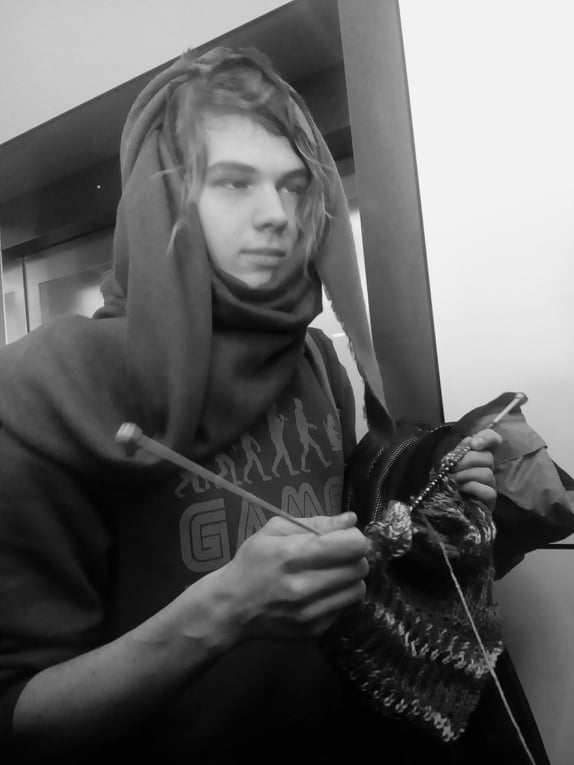
\includegraphics[width=8cm]{Sledz.jpg}\\
\vspace{1cm}
\Large{Śledź}
\end{center}
\newpage\begin{piosenka}[4mm]{Gimme Gimme Gimme -- ABBA}

\akordy{d  F a d} $\| \times 2$ \\[\zwrotkaspace]

Half past twelve & d \\
And I'm watching the late show in my flat all alone   & g \\
How I hate to spend the evening on my own  & g d \\
Autumn winds &   d \\
Blowing outside the window as I look around the room & g \\
And it makes me so depressed to see the gloom & g d \\
There's not a soul out there & B \\
No one to hear my prayer & g d A \\[\zwrotkaspace]

\refrenspace Gimme gimme gimme a man after midnight &   d B C d \\
\refrenspace Won't somebody help me chase these shadows awal & B d C d \\
\refrenspace Gimme gimme gimme a man after midnight &  d B C d \\
\refrenspace Take me through the darkness to the break of the Day & B d C d \\[\zwrotkaspace]

\akordy{d  F a d} $\| \times 2$ \\[\zwrotkaspace]

Movie stars & d \\
Find the end of the rainbow, with that fortune to win   & g \\
It's so different from the world I'm living In & g d \\
Tired of T.V. & d \\
I open the window and I gaze into the Wight   & g \\
But there's nothing there to see, no one in Wight & g d \\
There's not a soul out there & B \\
No one to hear my prayer & g d A \\[\zwrotkaspace]

Gimme gimme gimme a man after midnight\ldots & d B C d \\
Ah ah ah ah & B d C d \\
Gimme gimme gimme a man after midnight\ldots & d B C d \\
Ah ah ah ah & B d C d \\[\zwrotkaspace]

\akordy{D d C d} $\| \times 12$ \\[\zwrotkaspace]

There's not a soul out there & B \\
No one to hear my prayer & g d A \\[\zwrotkaspace]

\refrenspace Gimme gimme gimme\ldots $\| \times 2$ \\[\zwrotkaspace]

\akordy{d  F a d}

\end{piosenka}
\newpage\begin{piosenka}{Gold -- Imagine Dragons}

First comes the blessing of all that you've dreamed & a F \\
But then comes the curses of diamonds and rings \\
Only at first did it have its appeal \\
But now you can't tell the false from the real \\
Who can you trust? (Who can you trust) \\[\zwrotkaspace]

\refrenspace When everything, everything,  & a \\
\refrenspace Everything you touch turns to  & a \\
\refrenspace Gold, gold, gold & F \\
\refrenspace When everything, everything,  & C \\
\refrenspace Everything you touch turns to  & C \\
\refrenspace Gold, gold & d E \\
\refrenspace Gold & a F \\
\refrenspace Gold & a F \\
\refrenspace Gold & a F \\
\refrenspace Gold & a F \\[\zwrotkaspace]

Statues and empires are all at your hands, & a F \\
Water to wine and the finest of sands \\
When all that you have's turnin' stale and its cold, \\
Oh you'll no longer fear when your heart's turned to gold \\
Who can you trust (Who can you trust) \\[\zwrotkaspace]

\refrenspace When everything\ldots \\[\zwrotkaspace]

I'm dying to feel again, & d a d \\
Oh anything at all, & d a d \\
But oh I feel nothin', nothin', nothin', nothin' at all & d a \\[\zwrotkaspace]

\refrenspace When everything\ldots \\[\zwrotkaspace]

\end{piosenka}
\newpage{\small \begin{piosenka}{Hallelujah -- Leonard Cohen/Rufus Wainwright}
I've heard there was a secret chord & G e \\*
That David played, and it pleased the Lord & G e \\*
But you don't really care for music, do you? & C D G D \\*
It goes like this: the fourth, the fifth & G C D \\*
The minor fall, the major lift & e C \\*
The baffled king composing Hallelujah & D h e \\[1mm]

\refrenspace Hallelujah, hallelujah & C e \\*
\refrenspace Hallelujah, hallelujah & C G D G D \\[1mm]

Your faith was strong but you needed proof & G e \\*
You saw her bathing on the roof & G e \\*
Her beauty and the moonlight overthrew you & C D G D \\*
She tied you to a kitchen chair & G C D \\*
She broke your throne, she cut your hair & e C \\*
And from your lips she drew the Hallelujah & D h e \\[1mm]

\refrenspace Hallelujah\ldots \\[1mm]

Baby, I've been here before & G e \\*
I know this room, I've walked this floor & G e \\*
I used to live alone before I knew you & C D G D \\*
I've seen your flag on the marble arch & G C D \\*
Love is not a victory march & e C \\*
It's a cold and it's a broken Hallelujah & D h e \\[1mm]

\refrenspace Hallelujah\ldots \\[1mm]

There was a time you let me know & G e \\*
What's really going on below & G e \\*
But now you never show it to me, do you? & C D G D \\*
And remember when I moved in with you & G C D \\*
The holy dove was moving too & e C \\*
And every breath we drew was Hallelujah & D h e \\[1mm]

\refrenspace Hallelujah\ldots \\[1mm]

Maybe there’s a God above & G e \\*
But all I’ve ever learned from love & G e \\*
Was how to shoot at someone who outdrew you & C D G D \\*
It’s not a cry you can hear at night & G C D \\*
It’s not somebody who's seen the light & e C \\*
It’s a cold and it’s a broken Hallelujah & D h e \\[1mm]

\refrenspace Hallelujah\ldots \\*
\end{piosenka} }

\newpage\begin{piosenka}{House of gold -- Twenty One Pilots}

She asked me: ,,Son, when I grow old, & C \\
Will you buy me a house of gold? & C \\
And when your father turns to stone, & C \\
Will you take care of me?'' & C \\[\zwrotkaspace]

\refrenspace She asked me: ,,Son, when I grow old, & C F \\
\refrenspace Will you buy me a house of gold? & a G \\
\refrenspace And when your father turns to stone, & C F \\
\refrenspace Will you take care of me?'' & C G C \\[\zwrotkaspace]

\refrenspace I will make you & F A7 \\
\refrenspace Queen of everything you see & d b \\
\refrenspace I'll put you on the map & C \\
\refrenspace I'll cure you of disease & F C \\[\zwrotkaspace]

Let's say we up and left this town & C \\
And turned our future upside down & C \\
We'll make pretend that you and me & C \\
Lived ever after happily & C \\[\zwrotkaspace]

\refrenspace She asked me\ldots \\[\zwrotkaspace]

Oh, and since we know that dreams are dead & C \\
And life turns plans up on their head & C \\
I will plan to be a bum & C \\
So I just might become someone & C \\[\zwrotkaspace]

\refrenspace She asked me\ldots \\[\zwrotkaspace]

\end{piosenka}
\newpage\begin{piosenka}[3mm]{House of the Rising Sun -- Animals}
There is a house in New Orleans & a C D F \\
They call the Rising Sun & a C E \\
And it's been the ruin of many a poor boy & a C D F \\ 
And God I know I'm one & a E a C D F a E a E \\ [\zwrotkaspace]

My mother was a tailor & a C D F \\
Sewed my new blue jeans & a C E \\
My father was gamblin' man & a C D F \\ 
Down in New Orleans & a E a C D F a E a E \\ [\zwrotkaspace]

Now the only thing a gambler needs & a C D F \\
Is a suitcase and a trunk & a C E \\
And the only time he'll be satisfied & a C D F \\ 
Is when he's all a-drunk & a E a C D F a E a E \\ [\zwrotkaspace]

Oh mother, tell your children & a C D F \\
Not to do what I have done & a C E \\
Spend your lives in sin and misery & a C D F \\ 
In the house of the Rising Sun & a E a C D F a E a E \\ [\zwrotkaspace]

Well I've got one foot on the platform & a C D F \\
The other foot on the train & a C E \\
I'm going back to New Orleans & a C D F \\ 
To wear that ball and chain & a E a C D F a E a E \\ [\zwrotkaspace]

Well there is a house in New Orleans & a C D F \\
They call the Rising Sun & a C E \\
And it's been the ruin of many a poor boy & a C D F \\ 
And God I know I'm one & a E a C D F a E a E \\ 

\end{piosenka}
\newpage\begin{piosenka}{I can't help falling in love -- Elvis Presley}

\akordy{C G a C G} \\[\zwrotkaspace]
 
Wise men say, only fools rush In & C E a | F C G \\
But I can't help falling in love with you & F G a | F C G C \\[\zwrotkaspace]

Shall I  stay, would it be a sin? & C E a | F C G \\
If I can't help falling in love with you & F G a | F C G C \\[\zwrotkaspace]

\refrenspace Like a river flows surely to the sea & e H$^7$ e H$^7$ \\
\refrenspace Darling so it goes & e H$^7$ \\
\refrenspace Some things are meant to be & e A$^7$ d G \\[\zwrotkaspace]

Take my hand, take my whole life too & C E a | F C G \\
For I can't help falling in love with you & F G a | F C G C \\[\zwrotkaspace]

\refrenspace Like a river flows\ldots \\[\zwrotkaspace]

Take my hand, take my whole life too & C E a | F C G \\
For I can't help falling in love with you & F G a | F C G C \\
For I can't help falling in love with you & F G a | F C G C \\[\zwrotkaspace]

\end{piosenka}
\newpage\begin{piosenka_dluga}[2mm]{I see fire -- Ed Sheeran}

Oh, misty eye of the mountain below \\*
Keep careful watch of my brothers' souls \\*
And should the sky be filled with fire and smoke \\*
Keep watching over Durin's \\*
Sons & a \\[\zwrotkaspace]

\akordy{a C G F} $\| \times 2$ \\[\zwrotkaspace]

If this is to end in fire & a C \\*
Then we should all burn together & G F \\*
Watch the flames climb high into the night & a C G d \\*
Calling out father, oh, stand by and we will & a C G F \\*
Watch the flames burn auburn on the mountain side, high & d C F \\[\zwrotkaspace]

\akordy{a C G F} $\| \times 2$ \\[\zwrotkaspace]

And if we should die tonight & a C \\*
Then we should all die together & G F \\*
Raise a glass of wine for the last time & a C G d \\*
Calling out father, oh, prepare as we will & a C G F \\*
Watch the flames burn auburn on the mountain side & d C F \\*
Desolation comes upon the sky & d C F \\[\zwrotkaspace]

\refrenspace Now I see fire,  inside the mountains & a F G a \\*
\refrenspace I see fire,  burning the trees & a F G a \\*
\refrenspace And I see fire,  hollowing souls & a F G a \\*
\refrenspace I see fire,  blood in the breeze & a F G d \\*
\refrenspace And I hope that you'll remember me & d \\[\zwrotkaspace]

\akordy{a C G F} $\| \times 2$ \\[\zwrotkaspace]

Oh, should my people fall & a C \\*
Then surely I'll do the same & G F \\*
Confined in mountain halls & a C \\*
We got too close to the flame & G d \\*
Calling out father, oh, hold fast and we will & a C G F \\*
Watch the flames burn auburn on the mountain side & d C F \\*
Desolation comes upon the sky & d C F \\[\zwrotkaspace]

\refrenspace Now I see fire\ldots \\[\zwrotkaspace]

And if the night is burning & d a \\*
I will cover my eyes & C G \\*
For if the dark returns then & d a \\*
My brothers will die & C G \\*
And as the sky is falling down & d a \\*
It crashed into this lonely Town & C G \\*
And with that shadow upon the ground & d \\*
I hear my people screaming out & F G \\[\zwrotkaspace]

\refrenspace Now I see fire\ldots \\[\zwrotkaspace]

I see fire, oh you know I saw a city burning & a F G a	 \\*
I see fire, feel the heat upon my skin & a F G a \\*
And I see fire, oooooo (fire) & a F G a \\*
And I see fire burn auburn on the mountain side & a F G a \\[\zwrotkaspace]

\end{piosenka_dluga}


\newpage\begin{piosenka_dluga}{Каникулы -- Bum}

Все экзамены давно уже сданы & cis A \\
И учебники теперь мне не нужны & A E \\
И не надо рано утром мне вставать & E H \\
На учёбу убегать\ldots & H \\
Ооо\ldots \\[\zwrotkaspace]

Завтра я возьму билет на самолёт & cis A \\
О тебе мечтала весь учебный год & A E \\
Завтра я к тебе, любимый, прилечу & E H \\
Я давно к тебе хочу & H \\[\zwrotkaspace]

\refrenspace Каникулы, завтра я на всё забью & cis A \\
\refrenspace На учёбу не пойду, how do you do you do & E H \\
\refrenspace Каникулы, завтра я на всё забью & cis A \\
\refrenspace На учёбу не пойду, how do you do you do & E H \\[\zwrotkaspace]

Каникулы\ldots & cis A E H \\[\zwrotkaspace]

Завтра скажешь мне: ,,Любимая, привет! & cis A \\
Мы не виделись с тобою целый век & A E \\
Я тебе в ладошке солнце подарю'' & E H \\
И прошепчешь I love you & H \\[\zwrotkaspace]

Каждый день смогу с тобою рядом быть & cis A \\
И позволю на руках меня носить & A E \\
И позволю обнимать и целовать & E H \\
И любимой называть & H \\[\zwrotkaspace]

\newpage

\textbf{\large{Transkrypcja Каникулы}}\\[4mm]

\textit{Wsje ekzamieny dawno uże zdany} & cis A \\
\textit{I ucziebniki tiepier mnie nie nużny} & A E \\
\textit{I nie nada rano utrom mnie wstawać} & E H \\
\textit{Na uczjobu ubiegać\ldots} & H \\
\textit{Ooo\ldots} \\[\zwrotkaspace]

\textit{Zawtra ja wazmu biljet na samaljot} & cis A \\
\textit{O tiebie miecztała wies uczebnyj god} & A E \\
\textit{Zawtra ja k tiebie, ljubimyj, prilieczu} & E H \\
\textit{Ja dawno k tiebie chaczu} & H \\[\zwrotkaspace]

\textit{\refrenspace Kanikuły, zawtra ja na wsjo zablju} & cis A \\
\textit{\refrenspace Na uczjobu nie pajdu, how do you do you do} & E H \\
\textit{\refrenspace Kanikuły zawtra ja na wsjo zablju} & cis A \\
\textit{\refrenspace Na uczjobu nie pajdu, how do you do yo do} & E H \\[\zwrotkaspace]

\textit{Kanikuły\ldots} & cis A E H \\[\zwrotkaspace]

\textit{Zawtra skażesz mnie: ,,Ljubimaja, priwiet!} & cis A \\
\textit{My nie widielis c tabaju cjełyj wiek} & A E \\
\textit{Ja tiebie w ładoszkie sołce padarju''} & E H \\
\textit{I proszepczesz I love you} & H \\[\zwrotkaspace]

\textit{Każdyj dzjeń cmagu s toboju rjadom być} & cis A \\
\textit{I pazwolju na rukach mienia nasić} & A E \\
\textit{I pazwolju obnimać i cjełować} & E H \\
\textit{I ljubimoj nazywać} & H \\[\zwrotkaspace]

\textit{\refrenspace Kanikuły\ldots $\| \times 2$} \\[\zwrotkaspace]

\end{piosenka_dluga}
\newpage{\small \begin{piosenka}{Катюша}
	
Расцветали яблони и груши, & a E$^7$ \\
Поплыли туманы над рекой, & E$^7$ a \\
Выходила на берег Катюша & A$^7$ d a \\
На высокий берег на крутой! $\| \times 2$ & d a E$^7$ a \\[\zwrotkaspace]

Выходила, песню заводила & a E$^7$ \\
Про степного сизого орла, & E$^7$ a \\
Про того, которого любила, & A$^7$ d a \\
Про того, чьи письма берегла. $\| \times 2$ & d a E$^7$ a \\[\zwrotkaspace]

Ой, ты песня, песенка девичья, & a E$^7$ \\
Ты лети за ясным солнцем вслед & E$^7$ a \\
И бойцу на дальнем пограничье & A$^7$ d a \\
От Катюши передай привет. $\| \times 2$ & d a E$^7$ a \\[\zwrotkaspace]

Пусть он вспомнит девушку простую, & a E$^7$ \\
Пусть услышит, как она поёт, & E$^7$ a \\
Пусть он землю бережёт родную, & A$^7$ d a \\
А любовь Катюша сбережёт. $\| \times 2$ & d a E$^7$ a \\[\zwrotkaspace]

Расцветали яблони и груши, & a E$^7$ \\
Поплыли туманы над рекой, & E$^7$ a \\
Выходила на берег Катюша & A$^7$ d a \\
На высокий берег на крутой!	$\| \times 2$ & d a E$^7$ a \\[\zwrotkaspace]
	
\end{piosenka}}\\
{\small 
	\begin{tabular}{@{\hspace{3mm}}l@{\hspace{8mm}}>{\bfseries}l}
		\textit{Rascwietali jabłani i gruszy,} & a E$^7$ \\
		\textit{Papłyli tumany nad riekoj; }& E$^7$ a \\
		\textit{Wychadiła na bierieg Katiusza,} & A A$^7$ d a \\
		\textit{Na wysokij bierieg, na krutoj.} $\| \times 2$ & d a E$^7$ a \\[1mm]
		
		\textit{Wychadiła, piesniu zawadiła} & a E$^7$ \\
		\textit{Pra stiepnowa sizawa arła,} & E$^7$ a \\
		\textit{Pra tawo, katorawa liubiła,} & A A$^7$ d a \\
		\textit{Pra tawo, ćji pis'ma bieriegła.} $\| \times 2$ & d a E$^7$ a \\[1mm]
		
		\textit{Oj, ty piesnia, piesienka diewićja,} & a E$^7$ \\
		\textit{Ty leti za jasnym soncem wslied,} & E$^7$ a \\
		\textit{I bajcu na dalniem pogranićje} & A A$^7$ d a \\
		\textit{Ot Katiuszy pieriedaj priwiet.} $\| \times 2$ & d a E$^7$ a \\[1mm]
		
		\textit{Pust' on wspomnit diewuszku prastuju,} & a E$^7$ \\
		\textit{Pust' usłyszyt, kak ana pajot,} & E$^7$ a \\
		\textit{Pust' on ziemlju bierieżot radnuju} & A A$^7$ d a \\
		\textit{A liubow' Katiusza sbierieżot.} $\| \times 2$ & d a E$^7$ a \\[1mm]
		
		\textit{Rascwietali jabłani i gruszy\ldots} \\
		
	\end{tabular}

 }
\newpage{\small \begin{piosenka}{Lemon Tree -- Fool's Garden}
I'm sitting here in the boring room & e h \\*
It's just another rainy Sunday afternoon & e h \\*
I'm wasting my time, I got nothing to do & e h \\*
I'm hanging around, I'm waiting for you & e h \\*
But nothing ever happens and I wonder & a h e \\[\zwrotkaspace]

I'm driving around in my car & e h \\*
I'm driving too fast, I'm driving too far & e h \\*
I'd like to change my point of view & e h \\*
I feel so lonely, I'm waiting for you & e h \\*
But nothing ever happens and I wonder & a h e \\[\zwrotkaspace]

\refrenspace I wonder how, I wonder why & G D \\*
\refrenspace Yesterday you told me 'bout the blue blue sky & e h \\*
\refrenspace And all that I can see is just a yellow lemon tree & C D G D \\*
\refrenspace I'm turning my head up and down & G D \\*
\refrenspace I'm turning turning turning turning turning around & e h \\*
\refrenspace And all that I can see is just another lemon tree & C D G D \\[\zwrotkaspace]

I'm sitting here, I miss the power & e h \\*
I'd like to go out taking a shower & e h \\*
But there's a heavy cloud inside my head & e h \\*
I feel so tired put myself into bed & e h \\*
Well, nothing ever happens and I wonder & a h e \\[\zwrotkaspace]

Isolation is not good for me & H e \\*
Isolation, I don't want to sit on the lemon tree & D G H \\[\zwrotkaspace]

I'm steppin' around in the desert of joy & e h \\*
Baby, anyhow I'll get another toy & e h \\*
And everything will happen and you wonder & a h e \\[\zwrotkaspace]

\refrenspace I wonder how, I wonder why & G D \\*
\refrenspace Yesterday you told me 'bout the blue blue sky & e h \\*
\refrenspace And all that I can see is just another lemon tree & C D G D \\*
\refrenspace I'm turning my head up and down & G D \\*
\refrenspace I'm turning turning turning turning turning around & e h \\*
\refrenspace And all that I can see is just a yellow lemon tree & C D G D \\*
\refrenspace I wonder how, I wonder why & G D \\*
\refrenspace Yesterday you told me 'bout the blue blue sky & e h \\*
\refrenspace And all that I can see & C D \\*
\refrenspace And all that I can see & C D \\*
\refrenspace And all that I can see is just a yellow lemon tree & C D G \\*
\end{piosenka} }

\newpage\begin{piosenka_dluga}{Let her Go -- Passenger}

\refrenspace Well, you only need the light when it's burning low & a F C \\
\refrenspace Only miss the sun when it starts to snow & G  a \\
\refrenspace Only know you love her when you let her go & F C G \\
\refrenspace Only know you've been high when you're feeling low & F C \\
\refrenspace Only hate the road when you're missin' Home & G a \\
\refrenspace Only know you love her when you let her go & F C \\[\zwrotkaspace]

And you let her go & G \\[\zwrotkaspace]

\akordy{a   F   G   e} \\
\akordy{a   F   G} \\[\zwrotkaspace]

Staring at the bottom of your glass  & a F \\
Hoping one day you will make a dream last & G e \\
The dreams come slow and they go so fast & a F G \\
You see her when you close your eyes & a F \\
Maybe one day you will understand why & G e \\
Everything you touch surely dies & a F G \\[\zwrotkaspace]

\refrenspace But, you only need the light\ldots \\[\zwrotkaspace]

Staring at the ceiling in the dark  & a F  \\
Same old empty feeling in your heart   & G e \\
Love comes slow and it goes so fast   & a F G  \\
Well you see her when you fall asleep &  a F \\
But to never to touch and never to keep & G e \\
Because you loved her too much & a  \\
And you dived too deep & F G \\[\zwrotkaspace]

\refrenspace Cause, you only need the light\ldots \\[\zwrotkaspace]

And you let her go & a \\
Ooo ooo & F G \\
And you let her go &  a \\
Ooo ooo & F G \\
And you let her go & a F G e \\[\zwrotkaspace]

\akordy{a   F   G} \\[\zwrotkaspace]

\refrenspace Well, you only need the light when it's burning low & a F C \\
\refrenspace Only miss the sun when it starts to snow & G  a \\
\refrenspace Only know you love her when you let her go & F C G \\
\refrenspace Only know you've been high when you're feeling low & F C \\
\refrenspace Only hate the road when you're missin' Home & G a \\
\refrenspace Only know you love her when you let her go & F C \\[\zwrotkaspace]

\refrenspace Cause, you only need the light\ldots \\[\zwrotkaspace]

And you let her go  & G \\[\zwrotkaspace]

\end{piosenka_dluga}
\newpage\begin{piosenka}{Never gona give you up -- Rick Astley}

\akordy{G A fis h} \\[\zwrotkaspace]

We're no strangers to love & G A \\
You know the rules and so do I & G A \\
A full commitment's what I'm thinking of & G A \\
You wouldn't get this from any other guy & G A \\[\zwrotkaspace]

I just wanna tell you how I'm feeling & G A \\
Gotta make you understand & G A \\[\zwrotkaspace]

\refrenspace Never gonna give you up & G A \\
\refrenspace Never gonna let you down & fis h \\
\refrenspace Never gonna run around and desert you & G A fis h \\
\refrenspace Never gonna make you cry & G A \\
\refrenspace Never gonna say goodbye & fis h \\
\refrenspace Never gonna tell a lie and hurt you & G A fis h \\[\zwrotkaspace]

We've known each other for so long & G A \\
Your heart's been aching but you're too shy to say it & G A \\
Inside we both know what's been going on & G A \\
We know the game and we're gonna play it & G A \\[\zwrotkaspace]

And if you ask me how I'm feeling & G A \\
Don't tell me you're too blind to see & G A \\[\zwrotkaspace]

\refrenspace Never gonna give you up\ldots \\[\zwrotkaspace]

We've known each other for so long & G A \\
Your heart's been aching but you're too shy to say it & G A \\
Inside we both know what's been going on & G A \\
We know the game and we're gonna play it & G A \\[\zwrotkaspace]

I just wanna tell you how I'm feeling & G A \\
Gotta make you understand & G A \\[\zwrotkaspace]

\refrenspace Never gonna give you up\ldots  $\|\times2$ \\[\zwrotkaspace]

\end{piosenka}
\newpage\begin{piosenka}{Oops, I did it again -- Britney Spears}

Yeah yeah yeah yeah yeah $\| \times 2$ & cis cis \\[\zwrotkaspace]

I think I did it again & cis --- cis \\
I made you believe & cis A \\
were more than just friends (Oh baby) & A Gis \\
It might seem like a crush & cis Gis cis \\
But it doesn't mean that I'm serious & A Gis \\[\zwrotkaspace]

cause to lose all my senses & A Gis \\
That is just so typically me & A H \\
Oh baby, baby & H \\[\zwrotkaspace]

\refrenspace Oops!\ldots I did it again & cis Gis cis \\
\refrenspace I played with your heart, got lost in the game & H E H E \\
\refrenspace Oh baby, baby & H \\
\refrenspace Oops!\ldots you think I'm in love & cis Gis cis \\
\refrenspace That I'm sent from above & H E \\
\refrenspace I'm not that Innocent & Gis \\[\zwrotkaspace]

You see my problem is this & cis --- cis \\
I'm dreaming away & cis A \\
Wishing that heroes, they truly exist & A Gis \\
I cry, watching the days & cis Gis cis \\
Cant you see I'm a fool in so many ways & A Gis \\[\zwrotkaspace]

cause to lose all my senses & A Gis \\
That is just so typically me & A H \\
Oh baby, baby & H \\[\zwrotkaspace]

\refrenspace Oops!\ldots I did it again\ldots \\[\zwrotkaspace]

\end{piosenka}
\newpage\begin{piosenka}{Pumped Up Kicks -- Foster the People}

Robert's got a quick hand & e G \\
He'll look around the room, & D \\
He won't tell you his plan & A \\
He's got a rolled cigarette, & e G \\
Hanging out his mouth he's a cowboy kid & D A \\
Yeah found a six shooter gun & e G \\
In his dad's closet hidden in a box of fun things, & D A \\
I don't even know what & e G \\
But he's coming for you, & D \\
Yeah he's coming for you & A \\[\zwrotkaspace]
	
\refrenspace All the other kids with the pumped up kicks & e G D A \\
\refrenspace You'd better run, better run, out run my gun \\
\refrenspace All the other kids with the pumped up kicks \\
\refrenspace You'd better run, better run, faster than my bullet \\
\refrenspace $\| \times 2$ \\[\zwrotkaspace]

Daddy works a long day & e G \\
He be coming home late, & D \\
He's coming home late & A \\
And he's bringing me a surprise & e G \\
'Cause dinner's in the kitchen and it's packed in ice & D A \\
I've waited for a long time & e G \\
Yeah the slight of my hand is now a quick pull trigger & D A \\
I reason with my cigarette & e G \\
And say your hair's on fire, & D \\
You must have lost your wits, yeah & A \\[\zwrotkaspace]

\refrenspace All the other kids\ldots $\| \times 4$ \\[\zwrotkaspace]

\end{piosenka}
\newpage\begin{piosenka}[0mm]{Riptide -- Vance Joy}

\akordy{a G C} \\[\zwrotkaspace]

I was scared of dentists and the dark & a G C \\
I was scared of pretty girls and starting conversations \\
Oh, all my friends are turning green \\
You're the magician's assistant in their Dreas \\
Oh \\
Oh and they come unstuck \\[\zwrotkaspace]

\refrenspace Lady, running down to the riptide & a G C \\
\refrenspace Taken away to the dark side & C a \\
\refrenspace I wanna be your left hand Man & G C \\
\refrenspace I love you when you're singing that song and & a G C \\
\refrenspace I got a lump in my throat 'cause & C a \\
\refrenspace You're gonna sing the words wrong & G C \\[\zwrotkaspace]

There’s this movie that I think you'll like & a G C \\
This guy decides to quit his job and heads to New York City \\
This cowboy's running from himself \\
And she's been living on the highest shelf \\
Oh \\
Oh and they come unstuck \\[\zwrotkaspace]

\refrenspace Lady, running down to the riptide\ldots \\[\zwrotkaspace]

I just wanna, I just wanna know & a G \\
If you're gonna, if you're gonna stay & C F \\
I just gotta, I just gotta know & a G \\
I can't have it, I can't have it any other way & C F \\
I swear she's destined for the screen & a G C \\
Closest thing to Michelle Pfeiffer that you've ever seen, oh & a G C \\[\zwrotkaspace]

\refrenspace Lady, running down to the riptide\ldots $\| \times 3$ \\[\zwrotkaspace]

I got a lump in my throat ‘cause & C a \\
you're gonna sing the words wrong & G C \\[\zwrotkaspace]

\end{piosenka}
\newpage\begin{piosenka_dluga}{Shape of you -- Ed Sheeran}

The club isn't the best place to find a lover & h e \\*
So the bar is where I go & G A \\*
Me and my friends at the table doing shots \\*
Drinking fast and then we talk slow \\*
Come over and start up a conversation with just me \\*
And trust me I'll give it a chance now \\*
Take my hand, stop, put Van the Man on the jukebox \\*
And then we start to dance, and now I'm singing like \\[\zwrotkaspace]
	
\refrenspace Girl, you know I want your love & h e \\*
\refrenspace Your love was handmade for somebody like me & G A \\*
\refrenspace Come on now, follow my lead \\*
\refrenspace I may be crazy, don't mind me \\*
\refrenspace Say, boy, let's not talk too much \\*
\refrenspace Grab on my waist and put that body on me  \\*
\refrenspace Come on now, follow my lead \\*
\refrenspace Come, come on now, follow my lead \\*
\refrenspace  I'm in love with the shape of you \\*
\refrenspace We push and pull like a magnet do \\*
\refrenspace Although my heart is falling too \\*
\refrenspace I'm in love with your body \\*
\refrenspace And last night you were in my room \\*
\refrenspace And now my bedsheets smell like you \\*
\refrenspace Every day discovering something brand new \\*
\refrenspace I'm in love with your body \\*
\refrenspace $\|$ Oh—I—oh—I—oh—I—oh—I \\*
\refrenspace I'm in love with your body $\| \times 3$ \\*
\refrenspace Every day discovering something brand new \\*
\refrenspace I'm in love with the shape of you \\[\zwrotkaspace]

One week in we let the story begin \\*
We're going out on our first date \\*
You and me are thrifty, so go all you can eat \\*
Fill up your bag and I fill up a plate \\*
We talk for hours and hours about the sweet and the sour \\*
And how your family is doing okay \\*
Leave and get in a taxi, then kiss in the backseat \\*
Tell the driver make the radio play, and I'm singing like \\[\zwrotkaspace]

\refrenspace Girl, you know I want your love\ldots \\[\zwrotkaspace]

Come on, be my baby, come on $\| \times 4$ \\[\zwrotkaspace]

I'm in love with the shape of you \\*
We push and pull like a magnet do \\*
Although my heart is falling too \\*
I'm in love with your body \\*
Last night you were in my room \\*
And now my bedsheets smell like you \\*
Every day discovering something brand new \\*
I'm in love with your body \\*
Come on, be my baby, come on $\| \times 4$ \\*
Every day discovering something brand new \\*
I'm in love with the shape of you \\[\zwrotkaspace]

\end{piosenka_dluga}
\newpage\begin{piosenka_dluga}{Shut up and dance with me -- Walk the Moon}

\refrenspace Oh don't you dare look back & D G \\*
\refrenspace Just keep your eyes on me & h A \\*
\refrenspace I said you're holding back & D G \\*
\refrenspace She said shut up and dance with me & h A \\*
\refrenspace This woman is my destiny & D G h A \\*
\refrenspace She said oh oh oh & D G \\*
\refrenspace Shut up and dance with me & h A \\*[1mm]

We were victims of the night & D G h A \\*
The chemical, physical, kryptonie & D G h A \\*
Helpless to the bass and the fading light & D G h A \\*
Oh we were bound to get together & D G \\* 
Bound to get together & h A \\*
She took my arm & D G \\*
I don't know how it happener & h A \\*
We took the floor and she Said & D G h A \\*[1mm]

\refrenspace Oh don't you dare\ldots \\[1mm]

A backless dress and some beat up sneaks & D G h A \\*
My discotheque Juliet teenage dream & D G h A \\*
I felt it in my chest as she looked at me & D G h A \\*
I knew we were bound to be together & D G \\*
Bound to be together & h A \\*
She took my arm & D G \\*
I don't know how it happened & h A \\*
We took the floor and she said & D G h A \\*[1mm]

\refrenspace Oh don't you dare\ldots \\[1mm]

Deep in her eses & D G \\*
I think I see the future & h A \\*
I realize this is my last chance & D G h A \\*
She took my arm & D G \\*
I don't know how it happener & h A \\*
We took the floor and she Said & D G h A \\*[1mm]

\refrenspace Oh don't you dare\ldots $\| \times 2$ \\[1mm]

Oh oh oh shut up dance with me & D G h A \\*
Oh oh oh shut up dance with me & D G h A \\*

\end{piosenka_dluga}
\newpage\begin{piosenka_dluga}{Something just like this -- The Chainsmokers \& Coldplay}

\akordy{G A h} \\[\zwrotkaspace]

I've been reading books of old & h G \\*
The legends and the myths & A h \\*
Achilles and his gold \\*
Hercules and his gifts \\*
Spiderman's control \\*
And Batman with his fists \\*
And clearly I don't see myself upon that list \\[\zwrotkaspace]

But she said, where'd you wanna go? \\*
How much you wanna risk? \\*
I'm not looking for somebody \\*
With some superhuman gifts \\*
Some superhero \\*
Some fairytale bliss \\*
Just something I can turn to \\*
Somebody I can Kiss \\[\zwrotkaspace]

\refrenspace I want something just like this & h G\\*
\refrenspace Doo-doo-doo, doo-doo-doo & A h\\*
\refrenspace Doo-doo-doo, doo-doo-doo & G A\\*
\refrenspace $\| \times 2$ \\[\zwrotkaspace]

Oh, I want something just like this \\*
I want something just like this \\[\zwrotkaspace]

I've been reading books of old \\*
The legends and the myths \\*
The testaments they told \\*
The moon and its eclipse \\*
And Superman unrolls \\*
A suit before he lifts \\*
But I'm not the kind of person that it fits \\[\zwrotkaspace]

She said, where'd you wanna go? & h G \\*
How much you wanna risk? & A h \\*
I'm not looking for somebody \\*
With some superhuman gifts \\*
Some superhero \\*
Some fairytale bliss \\*
Just something I can turn to \\*
Somebody I can miss \\*
I want something just like this \\*
I want something just like this \\[\zwrotkaspace]

\refrenspace I want something just like this & h G\\*
\refrenspace Doo-doo-doo, doo-doo-doo & A h\\*
\refrenspace Doo-doo-doo, doo-doo-doo & G A\\*
\refrenspace $\| \times 2$ \\[\zwrotkaspace]

Where'd you wanna go? \\*
How much you wanna risk? \\*
I'm not looking for somebody \\*
With some superhuman gifts \\*
Some superhero \\*
Some fairytale bliss \\*
Just something I can turn to \\*
Somebody I can kiss \\*
I want something just like this \\*
Oh, I want something just like this \\*
Oh, I want something just like this \\*
Oh, I want something just like this \\[\zwrotkaspace]

\end{piosenka_dluga}
\newpage\begin{piosenka}{Somewhere over the Rainbow -- Israel ,,IZ'' Kamakawiwo'ole}
Oooo, oooo, oooo, oooo\ldots & G h C G \\
Oooo, oooo, oooo, oooo\ldots & C H$^7$ e C \\[\zwrotkaspace]
 
Somewhere over the rainbow, way up high & G h C G \\
and the dreams that you dream & C G \\
of once in a lullaby. Ohhhh. & D e C \\[\zwrotkaspace]
 
Somewhere over the rainbow bluebirds fly & G h C G \\
and the dreams that you dreamed of, & C G \\
dreams really do come true. Ohhhh. & D e C \\[\zwrotkaspace]
 
\refrenspace Someday I'll wish upon a star, & G \\
\refrenspace wake up where the clouds are far behind me. & h e C \\
\refrenspace Where troubles melts like lemon drops, & G \\
\refrenspace high above the chimney tops, & h \\
\refrenspace that's where you'll find me. & e C \\[\zwrotkaspace]
 
Somewhere over the rainbow, bluebirds fly & G h C G \\
and the dreams that you dare to, oh, why, & C G \\
oh why can't I? Ohhhh. & D e C \\[\zwrotkaspace]
 
\refrenspace Someday I'll wish upon a star\ldots \\[\zwrotkaspace]

Somewhere over the rainbow, bluebirds fly & G h C G \\
and the dreams that you dare to, oh, why, & C G \\
oh why can't I? Ohhhh. & D e C \\[\zwrotkaspace]

Oooo, oooo, oooo, oooo\ldots & G h C G \\
Oooo, oooo, oooo, oooo\ldots & C H$^7$ e C \\
\end{piosenka}
\newpage\begin{piosenka_dluga}[2mm]{Stayin' alive -- Bee Gees}

Well, you can tell by the way I use my walk & fis \\*
I'm a woman's man, no time to talk & fis E \\*
Music loud and women warm, I've been kicked around & fis \\*
Since I was born & fis E \\[\zwrotkaspace]

And now it's alright, it's okay & H \\*
And you may look the other way & H \\*
We can try to understand & H \\*
The New York Times' effect on man & H \\[\zwrotkaspace]

\refrenspace Whether you're a brother or whether you're a mother & fis \\*
\refrenspace You're stayin' alive, stayin' alive & fis \\*
\refrenspace Feel the city breakin' and everybody shakin' & fis \\*
\refrenspace And we're stayin' alive, stayin' alive & fis \\*
\refrenspace Ah, ha, ha, ha, stayin' alive, stayin' alive & fis \\*
\refrenspace Ah, ha, ha, ha, stayin' alive & fis E fis cis fis \\[\zwrotkaspace]

Well now, I get low and I get high & fis \\*
And if I can't get either, I really try & fis E \\*
Got the wings of heaven on my shoes & fis \\*
I'm a dancin' man and I just can't lose & fis E \\[\zwrotkaspace]

You know it's alright, it's okay & H \\*
I'll live to see another day & H \\*
We can try to understand & H \\*
The New York Times' effect on man & H \\[\zwrotkaspace]

\refrenspace Whether you're a brother\ldots \\[\zwrotkaspace]

Life goin' nowhere, somebody help me & B \\*
Somebody help me, yeah & B fis \\*
Life goin' nowhere, somebody help me, yeah & B fis \\*
I'm stayin' alive & fis \\[\zwrotkaspace]

Well, you can tell by the way I use my walk & fis \\*
I'm a woman's man, no time to talk & fis E \\*
Music loud and women warm, I've been kicked around & fis \\*
Since I was born & fis E \\[\zwrotkaspace]

And now it's alright, it's okay & H \\*
And you may look the other way & H \\*
We can try to understand & H \\*
The New York Times' effect on man & H \\[\zwrotkaspace]

\refrenspace Whether you're a brother or whether you're a mother & fis \\*
\refrenspace You're stayin' alive, stayin' alive & fis \\*
\refrenspace Feel the city breakin' and everybody shakin' & fis \\*
\refrenspace And we're stayin' alive, stayin' alive & fis \\*
\refrenspace Ah, ha, ha, ha, stayin' alive, stayin' alive & fis \\*
\refrenspace Ah, ha, ha, ha, stayin' alive & fis E fis cis fis \\[\zwrotkaspace]

Life goin' nowhere, somebody help me & B \\*
Somebody help me, yeah & B fis \\*
Life goin' nowhere, somebody help me, yeah & B fis \\*
I'm stayin' alive & fis \\[\zwrotkaspace]

\end{piosenka_dluga}
\newpage\begin{piosenka}{Take on me -- a-ha}

\akordy{h E A D A} \\
\akordy{h E D E} \\[\zwrotkaspace]

We're talking away & h E \\
I don't know what I'm to say & A D A \\
I'll say it anyway & h E \\
Today's another day to find you & A D A \\
Shying away & h E \\
I'll be coming for your love, okay? & fis D \\[\zwrotkaspace]

\refrenspace Take on me (take on me) & A E fis D \\
\refrenspace Take me on (take on me) & A E fis D \\
\refrenspace I'll be gone & A E fis D \\
\refrenspace In a day or two & A E D E \\[\zwrotkaspace]

So needless to say & h E \\
I'm odds and ends, but I'll be & A D A \\
stumbling away & h E \\
Slowly learning that life is okay & A D A \\
Say after me & h E \\
It's no better to be safe than sorry & fis D \\[\zwrotkaspace]

\refrenspace Take on me\ldots \\[\zwrotkaspace]

\end{piosenka}
\newpage\begin{piosenka}{The night we met -- Lord Huron}

I am not the only traveler & a G C \\
Who has not repaid his debt & a C F \\
I've been searching for a trail to follow again & a G C \\
Take me back to the night we met & a C F \\[\zwrotkaspace]
	
And then I can tell myself & a G C \\
What the hell I'm supposed to do & a C F \\
And then I can tell myself & a G C \\
Not to ride along with you & a C F \\[\zwrotkaspace]

\refrenspace I had all and then most of you & a \\
\refrenspace Some and now none of you & G C \\
\refrenspace Take me back to the night we met & a C F \\
\refrenspace I don't know what I'm supposed to do & a \\
\refrenspace Haunted by the ghost of you & G C \\
\refrenspace Oh, take me back to the night we met & a C F \\[\zwrotkaspace]

When the night was full of terrors & a G C \\
And your eyes were filled with tears & a C F \\
When you had not touched me yet & a G C \\
Oh, take me back to the night we met & a C F \\[\zwrotkaspace]

\end{piosenka}
\newpage\begin{piosenka_dluga}[4mm]{Toss a Coin to Your Witcher -- Joey Batey}
\textit{kapodaster na I progu}\\[\zwrotkaspace]

When a humble bard graced a ride along & a D d \\
With Geralt of Rivia along came this song & e D e E \\
From when the White Wolf fought a silver-tongued devil & a D \\
His army of elves at his hooves did they revel & G D G E \\[\zwrotkaspace]
 
They came after me with masterful deceit & a D d \\
Broke down my lute and they kicked in my teeth & G E a \\
While the devil’s horns minced our tender meat & a D d \\
And so cried the Witcher ``He can’t be bleat'' & G G E \\[\zwrotkaspace]
 
\refrenspace Toss a coin to your Witcher & a E C \\
\refrenspace O’ Valley of Plenty $\|\times2$ Oh, oh, oh & D a \\
\refrenspace Toss a coin to Your Witcher & a E C \\
\refrenspace O’ Valley of Plenty & D E \\[\zwrotkaspace]
 
At the edge of the world fight the mighty horde & a D F \\
That bashes and breaks you and brings you to mourn & G D G E \\
He thrust every elf far back on the shelf & a D F \\
High up on the mountain from whence it came & G D G E \\[\zwrotkaspace]

He wiped out your pest got kicked in his chest & a D F \\
He’s a friend of humanity so give him the rest & G E a \\
That’s my epic tale our champion prevailed & a D F \\
Defeated the villain now pour him some ale & G \\[\zwrotkaspace]
 
\refrenspace Toss a coin to your Witcher & a E C \\
\refrenspace O’ Valley of Plenty $\|\times2$ Oh, oh, oh & D a \\
\refrenspace Toss a coin to your Witcher & a E C \\
\refrenspace A friend of humanity & D E \\[\zwrotkaspace]
\end{piosenka_dluga}
\newpage\begin{piosenka}{Grosza daj Wiedźminowi -- Marcin Franc}
\textit{kapodaster na I progu}\\[\zwrotkaspace]

Tę balladę wam śpiewa skromny bard & a D d \\
Co z Geraltem z Rivii wyruszył na szlak & e D e E \\
Diaboła spotkał tam, co szukał z nim zwady & a D \\
I z elfów hufcami urządzał biesiady & G D G E \\[\zwrotkaspace]

Pochwycili mnie podstępem, no bo jak?! & a D d \\
Zniszczyli mi lutnię, skopali jak psa! & G E a \\
Ciała nasze dźgał ten rogaty stwór, & a D d \\
Zapłakał nasz wiedźmin, ,,Mam dosyć już!'' & G G E \\[\zwrotkaspace]

\refrenspace Grosza daj Wiedźminowi, & a E C \\
\refrenspace Sakiewką potrząśnij $\|\times2$ ło, o, o! & D a \\
\refrenspace Grosza daj Wiedźminowi, & a E C \\
\refrenspace Sakiewką potrząśnij! & D E \\[\zwrotkaspace]

Lecz chwycił Biały Wilk za morderczy róg, & a D F \\
Co tylu już przed nim obalił był z nóg & G D G E \\
Elfy cisnął precz, aż na górski szczyt, & a D F \\
Daleko od ludzi, gdzie miejsce ich & G D G E \\[\zwrotkaspace]

Choć oberwał sam, zmiażdżył bestii kark, & a D F \\
Ten obrońca ludzkości, toastu jest wart & G E a \\
Oto moja pieśń, to wasz bohater jest, & a D F \\
On wrogów pokonał, nalejcie mu więc! & G \\[\zwrotkaspace]

\refrenspace Grosza daj Wiedźminowi, & a E C \\
\refrenspace Sakiewką potrząśnij $\|\times2$ ło, o, o! & D a \\
\refrenspace Grosza daj Wiedźminowi, & a E C \\
\refrenspace Obrońcy ludzkości! & D E \\
\end{piosenka}
\newpage\begin{piosenka}{Kotlok dej Heksterowi -- Tomasz Kukułka?}
\textit{kapodaster na I progu}\\[\zwrotkaspace]

Tom pieśniczke wom śpiewo skromny bard, & a D d \\
Co z Gerltym ze Rivii poszoł wojować & e D e E \\
Czorta spotkoł tam, chcioł bić naszo dwójka, & a D \\
Z hordami goroli urządzoł barbórkal & G D G E \\[\zwrotkaspace]

Za frak mie chycili, ociulali mie fest, & a D d \\
Rozdupili mie lutnia, byłech jak pies & G E a \\
Ciała nasze dźgoł tyn rogoty stwór, & a D d \\
Poczuł ryczeć nasz hekser, co to za tempy ciul & G G E \\[\zwrotkaspace]

\refrenspace Kotlok dej hekserowi & a E C \\
\refrenspace Do kapsy mu pociś $\|\times2$ ŁoOHOhooooo & D a \\
\refrenspace Kotlok dej hekserowi & a E C \\
\refrenspace Do kapsy mu poćiiiiiiiiIIIIIIIIIiiiiiś. & D E \\[\zwrotkaspace]

Lecz chycił bioły wilk za pieruński róg & a D F \\
Co wiela już przed nim naklupoł w tyn dziób. & G D G E \\
Gorole cisną nazot, aż na hołdy wierch & a D F \\
Zdala od hanysów, kaj miejsce ich jest & G D G E \\[\zwrotkaspace]

Choć mu wklupali, diobłu trefił szlag, & a D F \\
Tyn obrońca Hanysów kolejki jest wort. & G E a \\
To pieśniczka mo to wasz bohaytr je, & a D F \\
On gorolom wdupi gorzoł niech leje sieeeeeee & G \\[\zwrotkaspace]

\refrenspace Kotlok dej hekserowi & a E C \\
\refrenspace Do kapsy mu pociś $\|\times2$ ŁoOOhooooo & D a \\
\refrenspace Kotlok dej hekserowi & a E C \\
\refrenspace On przaja Hanysom & D E \\
\end{piosenka}
\newpage\begin{piosenka}{Wake me up -- Avicii}

Feeling my way through the darkness & e C G D \\
Guided by a beating heart \\
I can't tell where the journey will end \\
But I know where to start \\[\zwrotkaspace]

They tell me I'm too young to understand \\
They say I'm caught up in a dream \\
Well life will pass me by if I don't open up my eyes \\
Well that's fine by me \\[\zwrotkaspace]
	
\refrenspace So wake me up when it's all over & e C G D \\
\refrenspace When I'm wiser and I'm older \\
\refrenspace All this time I was finding myself \\
\refrenspace And I didn't know I was lost \\[\zwrotkaspace]

I tried carrying the weight of the world \\
But I only have two hands \\
I hope I get the chance to travel the world \\
And I don't have any plans \\[\zwrotkaspace]

I wish that I could stay forever this young \\
Not afraid to close my eyes \\
Life's a game made for everyone \\
And love is a prize \\[\zwrotkaspace]

\refrenspace So wake me up\ldots $\| \times 2$ \\[\zwrotkaspace]

I didn't know I was lost $\| \times 4$ & h G D A \\[\zwrotkaspace]

\end{piosenka}
\newpage\begin{piosenka}{West coast -- Imagine Dragons}

\akordy{e C G} \\[\zwrotkaspace]

One more day we'll spend together & e C G \\
Lay your eyes, look up upon me for the better & e C G \\
Oh, I know I'm worse for weather & e C G \\
But my love, I won't give up & e D G \\[\zwrotkaspace]

Spend my days cursing my soul & e C G \\
Wishing I could paint my scars and make me whole & e C G \\
Oh, I know I could be better & e C G \\
But my love, I won't give up & e D G \\[\zwrotkaspace]

\refrenspace I ain't no superman, I ain't no holy gost & C G \\
\refrenspace I'm just the one that keeps you up at night, & D \\
\refrenspace You love the most & e \\
\refrenspace I'll be your strong man, I'll be your West Coast & C G \\
\refrenspace I'll be the sun, I'll be the waves, & D \\
\refrenspace I'll be the one you love the most & e \\
\refrenspace Ooh, hey, hey, hey, oh & C G \\
\refrenspace I'll be, I'll be, I'll be, I'll be, & D \\
\refrenspace I'll be your West Coast, honey & e \\
\refrenspace Ooh, hey, hey, hey, oh & C G \\
\refrenspace I'll be, I'll be, I'll be, I'll be, & D \\
\refrenspace I'll be your West Coast, honey & e \\[\zwrotkaspace]

\akordy{e C G} $\| \times 2$ \\[\zwrotkaspace]

I'd change my ways if you would stay & e C G \\
And all your tears that you have cried will go away & e C G \\
Oh, just grant me one more day & e C G \\
Oh, my love, please don't give up & e D G \\
See the devil at my door & e C G \\
I see the future of the ones that I've ignored & e C D \\
I guess I was born to be at war & e C G \\
But my love, I won't give up & e D G \\
So, my love, please don't give up & e D G \\[\zwrotkaspace]

\refrenspace I ain't no superman\ldots \\[\zwrotkaspace]

\end{piosenka}
\newpage\begin{piosenka}{What is love -- Haddaway}

\refrenspace What is love? Baby don't hurt me & a C \\
\refrenspace Don't hurt me no more & e G \\
\refrenspace & a \\
\refrenspace Baby don't hurt me, & C \\
\refrenspace Don't hurt me no more & e G \\[\zwrotkaspace]

\akordy{a C e G} \\[\zwrotkaspace]

What is love? & a \\[\zwrotkaspace]

\akordy{C e G}\\[\zwrotkaspace]

I don't know why you're not fair & a C e \\
I give you my love, but you don't care & e G a \\
So what is right and what is wrong? & a C e \\
Gimme a sign & e G \\[\zwrotkaspace]

\refrenspace What is love\ldots \\[\zwrotkaspace]

Ouoo $\| \times 2$ & a C e G \\[\zwrotkaspace]

Oh, I don't know, what can I do? & a C e \\
What else can I say, it's up to you & e G a \\
I know we're one, just me and you & a C e \\
I can't go on	e G \\[\zwrotkaspace]

\refrenspace What is love\ldots $\| \times 2$ \\[\zwrotkaspace]

Ouoo $\| \times 2$ & a C e G \\[\zwrotkaspace]

Don't hurt me & a a C \\
Don't hurt me & a a C \\[\zwrotkaspace]

\akordy{a C e G} \\[\zwrotkaspace]

I want no other, no other lover & a C e \\
This is our life, our time & e G a \\
We are together I need you forever & a C e \\
Is it love? & e G a \\[\zwrotkaspace]

\refrenspace What is love\ldots $\| \times 2$ \\[\zwrotkaspace]

What is love? & a \\[\zwrotkaspace]

\end{piosenka}
\newpage{\small \begin{piosenka}{Wind of Change -- Scorpions}

\akordy{F d F d* a* G* C!}\\[\zwrotkaspace]
I follow the Moskva & C d  \\*
Down to Gorky Park & d C  \\*
Listening to the wind of change & C d* a* G* C!  \\*
An August summer night & C d  \\*
Soldiers passing by & d C  \\*
Listening to the wind of change & C d* a* G*  \\[\zwrotkaspace]

\akordy{F d F d* a* G* C!}\\[\zwrotkaspace]

The world is closing in & C d  \\*
Did you ever think & d C  \\*
That we could be so close like brothers & C d* a* G* C!  \\*
The future's in the air & C d  \\*
I can feel it everywhere & d C  \\*
Blowing with the wind of change & C d* a* G*  \\[\zwrotkaspace]

\refrenspace Take me to the magic of the moment & C G d G  \\*
\refrenspace On a glory night & C G  \\*
\refrenspace Where the children of tomorrow dream away & d G a  \\*
\refrenspace In the wind of change & F G  \\[\zwrotkaspace]

Walking down the street & C d  \\*
Distant memories & d C  \\*
Are buried in the past forever & C d* a* G* C!  \\*
I follow the Moskva & C d  \\*
Down to Gorky Park & d C  \\*
Listening to the wind of change & C d* a* G*  \\[\zwrotkaspace]

\refrenspace Take me\ldots \\[\zwrotkaspace]

The wind of change blows straight & a G  \\*
Into the face of time & G a  \\*
Like a stormwind that will ring & a G  \\*
The freedom bell for peace of mind & G a  \\*
Let your balalaika sing & a C  \\*
What my guitar wants to say & e E$^7$  \\[\zwrotkaspace]

\refrenspace Take me\ldots \\[\zwrotkaspace]

\akordy{ F d F d a G C} \end{piosenka} }
\newpage{\small \begin{piosenka_dluga}{With or without you -- U2}

See the stone set in your eyes & D A h \\*
See the thorn twist in your side & h G D \\*
I'll wait for you & D A h G \\*
Sleight of hand and twist of fate & D A h \\*
On a bed of nails she makes me wait & h G D \\*
And I wait, without you & D A h G \\[\zwrotkaspace]

\refrenspace With or without you & G D A \\*
\refrenspace With or without you & A h G \\[\zwrotkaspace]

Through the storm we reach the shore & D A h \\*
You give it all but I want more & h G D \\*
And I'm waiting for you & D A h G \\[\zwrotkaspace]

\refrenspace With or without you & G D A \\*
\refrenspace With or without you & A h G \\*
\refrenspace I can't live & G D A \\*
\refrenspace With or without you & A h G \\*
\refrenspace And you give yourself away & G D A \\*
\refrenspace And you give yourself away & A h G \\*
\refrenspace And you give, and you give & G D A \\*
\refrenspace And you give yourself away & A h G \\[\zwrotkaspace]

My hands are tied & D A h \\*
My body bruised, she's got me with & h G D \\*
Nothing to win and & D A \\*
Nothing left to Lose & h G \\*
And you give yourself away & G D A \\*
And you give yourself away & A h G \\*
And you give, and you give & G D A \\*
And you give yourself away & A h G \\[\zwrotkaspace]

\refrenspace With or without you & G D A \\*
\refrenspace With or without you & A h G \\*
\refrenspace I can't live & G D A \\*
\refrenspace With or without you & A h G \\[\zwrotkaspace]

Oh & D A h G \\*
Oh & D A h G \\[\zwrotkaspace]

\refrenspace With or without you & G D A \\*
\refrenspace With or without you & A h G \\*
\refrenspace I can't live & G D A \\*
\refrenspace With or without you & A h G \\[\zwrotkaspace]

\end{piosenka_dluga} }
\newpage\begin{piosenka}{Zombie -- The Cranberries}
Another head hangs lowly & e C \\*
Child is slowly taken & G D \\*
And the violence caused such silence & e C \\*
Who are we mistaken & G D \\[\zwrotkaspace]
 
But you see, it's not me & e \\*
It's not my family & C \\*
In your head, in your head & G \\*
They are fighting & D \\[\zwrotkaspace]

\refrenspace With their tanks, and their bombs & e \\*
\refrenspace And their bombs, and their guns & C \\*
\refrenspace In your head, in your head & G \\*
\refrenspace They are cryin' & D \\*
\refrenspace In your head, in your head & e C \\*
\refrenspace Zombie, zombie, zombie & G D \\*
\refrenspace What's in your head, in your head & e C \\*
\refrenspace Zombie, zombie, zombie & G D \\[\zwrotkaspace]
 
Another mother's breakin' & e C \\*
Heart is taking over & G D \\*
When the violence causes silence & e C \\*
We must be mistaken & G D \\[\zwrotkaspace]
 
It's the same old theme & e \\*
Since 1916 & C \\*
In your head, in your head & G \\*
They're still fightin' & D \\[\zwrotkaspace]

\refrenspace With their tanks\ldots \\*
\end{piosenka}


\songssection{Inside i memy}{G.F. Darwin, Smash mouth\\ Rurczak Kurczak}
\newpage{\small \begin{piosenka_dluga}[5mm]{All Star -- Smash mouth}

Somebody once told me the world is gonna roll me & C G d F \\*
I ain't the sharpest tool in the shed & C G d F \\*
She was looking kind of dumb with her finger and her thumb & C G d F \\*
In the shape of an "L" on her forehead & C G d F \\[\zwrotkaspace]

Well the years start coming and they don't stop coming & C G \\*
Fed to the rules and I hit the ground running & d F \\*
Didn't make sense not to live for fun & C G \\*
Your brain gets smart but your head gets dumb & d F \\*
So much to do, so much to see & C G \\*
So what's wrong with taking the back streets? & d F \\*
You'll never know if you don't go & C G \\*
You'll never shine if you don't glow & d F \\[\zwrotkaspace]

\refrenspace Hey now, you're an all-star, get your game on, go play & C G d F \\*
\refrenspace Hey now, you're a rock star, get the show on, get paid & C G d F \\*
\refrenspace And all that glitters is gold & C G d F \\*
\refrenspace Only shooting stars break the mold & F C G d F \\[\zwrotkaspace]

It's a cool place and they say it gets colder & C G \\*
You're bundled up now, wait till you get older & d F \\*
But the meteor men beg to differ & C G \\*
Judging by the hole in the satellite picture & d F \\*
The ice we skate is getting pretty thin & C G \\*
The water's getting warm so you might as well swim & d F \\*
My world's on fire, how about yours? & C G \\*
That's the way I like it and I never get bored & d F \\[\zwrotkaspace]

\refrenspace Hey now, you're an all-star\ldots \\[\zwrotkaspace]

\refrenspace Hey now, you're an all-star, get your game on, go play & C G d F \\*
\refrenspace Hey now, you're a rock star, get the show, on get paid  & C G d F \\*
\refrenspace And all that glitters is gold & C G d F \\*
\refrenspace Only shooting stars & F C G d F \\[\zwrotkaspace]

Somebody once asked could I spare some change for gas? & C G d F \\*
I need to get myself away from this place & C G d F \\*
I said yep what a concept & C G \\*
I could use a little fuel myself & d F \\*
And we could all use a little change & C G d F \\[\zwrotkaspace]

Well, the years start coming and they don't stop coming & C G \\*
Fed to the rules and I hit the ground running & d F \\*
Didn't make sense not to live for fun & C G \\*
Your brain gets smart but your head gets dumb & d F \\*
So much to do, so much to see & C G \\*
So what's wrong with taking the back streets? & d F \\*
You'll never know if you don't go (go!) & C G \\*
You'll never shine if you don't glow & d F \\[\zwrotkaspace]

\refrenspace Hey now, you're an all-star, get your game on, go play & C G d F \\*
\refrenspace Hey now, you're a rock star, get the show on, get paid & C G d F \\*
\refrenspace And all that glitters is gold & C G d F \\*
\refrenspace Only shooting stars break the mold & F C G d F \\[\zwrotkaspace]

\refrenspace And all that glitters is gold & C G d F \\*
\refrenspace Only shooting stars break the mold & F C G d F \\

\end{piosenka_dluga} }
\newpage\begin{piosenka_dluga}{Coconut song -- Ryan Cayabyab, Smokey Mountain}

(Lalala ya lalala yayayayayayay) $\| \times 4$ & D G A \\*
(Co-conut cococococonut -- coconut) $\| \times 4$ & D G D A \\[\zwrotkaspace]

The coconut nut is a giant nut & D G \\*
If you eat too much, you'll get very fat (very fat) & A D \\*
Now, the coconut nut is a big, big nut & D G \\*
But this delicious nut is not a nut & A G D \\[\zwrotkaspace]

\refrenspace It's the coco fruit (it's the coco fruit) & A D \\*
\refrenspace Of the coco tree (of the coco tree) & A D \\*
\refrenspace From the coco palm family (yayayayaya) & A G D \\[\zwrotkaspace]

\refrenspace There are so many uses of the coconut tree& D G \\*
\refrenspace You can build a bigger house for the family & A D \\*
\refrenspace All you need is to find a coconut man & D G \\*
\refrenspace If he cuts the tree, he gets the fruits free & A G D \\*[\zwrotkaspace]

\refrenspace It's the coco fruit\ldots \\*[\zwrotkaspace]

\refrenspace (Co-conut cococococonut -- coconut) & D G A D \\*
\refrenspace (Co-conut cococococonut -- coconut) & G A G \\[\zwrotkaspace]

The coconut bark for the kitchen floor & D G \\*
If you save some of it, you can build a door & A D \\*
Now, the coconut trunk, do not throw this junk & D G \\*
If you save some of it, you'll have a second floor & A G D \\[\zwrotkaspace]

The coconut wood is very good & D G \\*
It can stand 20 years if you pray it wood & A D \\*
Now, the coconut root, to tell you the truth & D G \\*
You can throw it or use it as firewood & A G D \\[\zwrotkaspace]

The coconut leaves good shade it gives & D G \\*
For the roof, for the walls up against the eaves & A D \\*
Now, the coconut fruit, say my relatives & D G \\*
Make good cannonballs up against the thieves & A G D \\[\zwrotkaspace]

\refrenspace It's the coco fruit (it's the coco fruit) & A D \\*
\refrenspace Of the coco tree (of the coco tree) & A D \\*
\refrenspace From the coco palm family (yayayayaya) & A G D \\[\zwrotkaspace]

The coconut nut is a giant nut & D G \\*
If you eat too much, you'll get very fat & A D \\*
Now, the coconut nut is a big, big nut & D G \\*
But this delicious nut is not a nut & A G D \\[\zwrotkaspace]

The coconut nut is a giant nut & D G \\*
If you eat too much, you'll get very fat & A D \\*
Now, the coconut nut is a big, big nut & D G \\*
But this delicious nut is not a nut & A G D \\[\zwrotkaspace]

\refrenspace It's the coco fruit (it's the coco fruit) & A D \\*
\refrenspace Of the coco tree (of the coco tree) & A D \\*
\refrenspace From the coco palm family (yayayayaya) & A G D \\*
\refrenspace $\| \times 3$ \\[\zwrotkaspace]

 (Lalala la lala lala la) & D G \\*
(La la la lalala la la la lala) Olé! & A D \\

\end{piosenka_dluga}
\newpage\begin{piosenka_dluga}{Dance dance baby -- Rurczak Kurczak}

\akordy{e} \\*
\akordy{e G A e} \\*
\akordy{e G A e} \\[\zwrotkaspace]

When the stars come out around us & e G \\*
Music plays in our hearts & D A e \\*
I direct my vision into yea & e G \\*
Play and dancing starts & D A e \\[\zwrotkaspace]

\refrenspace \akordy{G A e} \\*
\refrenspace Dance dance babe \\*
\refrenspace \akordy{G A e} \\*
\refrenspace I wanna see \\*
\refrenspace \akordy{G A e} \\*
\refrenspace Dance dance babe \\*
\refrenspace I wanna see you dancing on the floor & G A H \\*
\refrenspace I wanna dance with you \\[\zwrotkaspace]

Hey (hey) I wanna dance with you babe & e G \\*
Oh dance with you babe & A \\*
All the night & e \\*
$\| \times 2$ \\[\zwrotkaspace]

\refrenspace \akordy{G A e} \\*
\refrenspace Dance dance\ldots \\[\zwrotkaspace]

\akordy{e G A e} \\*
\akordy{e G A e} \\[\zwrotkaspace]

You, your beauty intimidates me & e G \\*
You surely go to gym & D A e \\*
I am drinkin' now cup of tea & e G \\*
I couldn't find the rhym & D A e \\[\zwrotkaspace]

\refrenspace \akordy{G A e} \\*
\refrenspace Dance dance babe \\*
\refrenspace \akordy{G A e} \\*
\refrenspace I wanna see \\*
\refrenspace \akordy{G A e} \\*
\refrenspace Dance dance babe \\*
\refrenspace I wanna see you dancing on the floor & G A H \\*
\refrenspace And now guitar solo \\[\zwrotkaspace]

\akordy{e G A e} \\*
\akordy{e G A e} \\*
\akordy{G A e} \\*
\akordy{G A e} \\*
\akordy{G A e} \\*
\akordy{G A H} \\[\zwrotkaspace]

Hey (hey) I wanna dance with you babe & e G \\*
Oh dance with you babe & A \\*
All the night & e \\*
$\| \times 2$ \\[\zwrotkaspace]

\refrenspace \akordy{G A e} \\*
\refrenspace Dance dance\ldots \\[\zwrotkaspace] 

Hey (hey) I wanna\ldots

\end{piosenka_dluga}
\newpage\begin{piosenka_dluga}{Deja Vu -- Initial D}

\akordy{G A b} \\*
\akordy{G A E} \\*
\akordy{b A b A} \\*
\akordy{G A E Fis} \\[\zwrotkaspace]

\akordy{F G F G} $\| \times 2$ \\[\zwrotkaspace]

See your body into the moonlight & d \\*
Even if I try to cancel & B C \\*
All the pictures into the mind & d \\*
There's a flashing in my eyes & a B \\[\zwrotkaspace]

Don't you see my commission, the nation & B C \\*
Has gone running again & a B \\*
Can't you see now, illusions & B \\*
Right into your mind & C D \\[\zwrotkaspace]

\refrenspace Deja vu & B \\*
\refrenspace I've just been in this place before & C d \\*
\refrenspace Higher on the street & B \\*
\refrenspace And I know it's my time to go & C G \\*
\refrenspace Calling you, and the search is a mystery & B C d \\*
\refrenspace Standing on my feet & B \\*
\refrenspace It's so hard when I try to be me, woah & C G a \\[\zwrotkaspace]

\refrenspace Deja vu & B \\*
\refrenspace I've just been in this time before & C d \\*
\refrenspace Higher on the beat & B \\*
\refrenspace And I know it's a place to go & C G \\*
\refrenspace Calling you and the search is a mystery & B C d \\*
\refrenspace Standing on my feet & B \\*
\refrenspace It's so hard when I try to be me, yeah & C G a \\[\zwrotkaspace]

\akordy{F G F G} $\| \times 2$ \\[\zwrotkaspace]

See the future into the present & d \\*
See my past leaves in the distance & B C \\*
Try to guess now what's going on & d \\*
And the band begins to play & a B \\[\zwrotkaspace]

Don't you see my commission, the nation & B C \\*
Has gone running again & a B \\*
Can't you see now, illusions & B \\*
Right into your mind & C D \\[\zwrotkaspace]

\refrenspace Deja vu & B \\*
\refrenspace I've just been in this place before & C d \\*
\refrenspace Higher on the street & B \\*
\refrenspace And I know it's my time to go & C G \\*
\refrenspace Calling you, and the search is a mystery & B C d \\*
\refrenspace Standing on my feet & B \\*
\refrenspace It's so hard when I try to be me, woah & C G a \\[\zwrotkaspace]

\refrenspace Deja vu & B \\*
\refrenspace I've just been in this time before & C d \\*
\refrenspace Higher on the beat & B \\*
\refrenspace And I know it's a place to go & C G \\*
\refrenspace Calling you and the search is a mystery & B C d \\*
\refrenspace Standing on my feet & B \\*
\refrenspace It's so hard when I try to be me, yeah & C G a \\[\zwrotkaspace]

\akordy{F G F G} $\| \times 2$ \\[\zwrotkaspace]

See your body into the moonlight & d \\*
Even if I try to cancel & B C \\*
All the pictures into the mind & d \\*
There's a flashing in my eyes & a B \\[\zwrotkaspace]

Don't you see my commission, the nation & B C \\*
Has gone running again & a B \\*
Can't you see now, illusions & B \\*
Right into your mind & C D \\[\zwrotkaspace]

\refrenspace Deja vu\ldots \\[\zwrotkaspace]

\akordy{F G F G} $\| \times 4$ \\[\zwrotkaspace]

\end{piosenka_dluga}
\newpage\begin{piosenka}{Dotknij twarzy mej -- G.F. Darwin}

\akordy{fis h E Cis} \\[\zwrotkaspace]

Haj, heloł, hałar ju! & fis h \\
To po angielsku znaczy witaj piękna. & E Cis \\
Zrobię 20 pompek & fis h \\
I w 10 sekund wypijam wrzątek & E Cis \\[\zwrotkaspace]

Miłość ma słodki smak, jest jak batonik, & fis h \\
Albo banan, gruszka. & E Cis \\
Proszę Cię wciąż o jedno & fis h \\
Podaruj mi klucz Twojego serduszka & E Cis \\[\zwrotkaspace]

\refrenspace Dotknij twarzy mej palcami rąk & fis h \\
\refrenspace A ja dotknę potem Ciebie. & D Cis \\
\refrenspace Dotknę twarzy twej palcami dłoni swej & fis h \\
\refrenspace Byś z wrażenia upadła na ziemie. & D Cis \\
\refrenspace $\| \times 2$ \\[\zwrotkaspace]

Los do mnie śmieje się & fis h \\
Bo kiedy patrzę w twoje oczy dwoje & E Cis \\
Serce mi mocniej bije. & fis h \\
Bandytów powalam ciosem w szyje. & E Cis \\[\zwrotkaspace]

Dwanaście długich lat, & fis h \\
Po raz ostatni wtedy ją widziałem. & E Cis \\
Wyszła do toalety & fis h \\
Podobno śmierdziły mi skarpety. & E Cis \\[\zwrotkaspace]

\textit{Skarbie, od kiedy odeszłaś} \\
\textit{Czuję się jak żółw bez skorupy,} \\
\textit{Jak jednorożec bez roga\ldots rogu,} \\
\textit{Jak ptak bez dzioba, albo żyrafa bez szyi.} \\[\zwrotkaspace]

\refrenspace Dotknij twarzy mej\ldots \\[\zwrotkaspace]

\end{piosenka}
\newpage\begin{piosenka}{Intercontitnental bajers -- Solar \& Białas}

Seksturystyka jest zjawiskiem polegającym na tym, \\ 
że osoby z krajów zamożniejszych przemieszczają się \\
do krajów mniej zamożnych i korzystają tam z usług prostytutek \\[\zwrotkaspace]

Miał mięśnie jak skały, fale się odbijały \\
Postura koszykarza, świat dla niego był za mały \\
Dziewczyny wciąż się przy nim śmiały, to lubił \\
Dziewczyny się przy nim nie śmiały odmówić \\[\zwrotkaspace]

Tylko w jednym celu wciąż przemierzał kontynenty \\
Na insta licznik się przekręcił, kiedy zrobił selfie \\
Dziewczyny mdlały, gdy niby niechcący puszczał ręcznik \\
Piłka, żeby mu się przyjrzeć, aż stanęła na obręczy \\[\zwrotkaspace]

\refrenspace Europa, Ameryki, przez Australię do Afryki \\
\refrenspace Nie musi znać języków, żeby poznawać języki \\
\refrenspace On tylko ją zaliczył, to się liczy i się zmył \\
\refrenspace Nawet nie wiedziała, że to był \\
\refrenspace $\| \times 2$ \\[\zwrotkaspace]

\refrenspace Intercontinental Bajers, Intercontinental Bajers, \\
\refrenspace Intercontinental Bajers, Intercontinental Bajers \\
\refrenspace Ba-Ba-Ba-Ba-Ba-Ba-Bajers, Ba-Ba-Ba-Bajers \\[\zwrotkaspace]

Intercontinental Bajers, Bajers, Bajers \\
Intercontinental Bajers \\[\zwrotkaspace]

W Chorwacji w desperacji raz podjechał do dwóch dupek \\
Od tamtej pory trójkąt to dla niego norma (głupek) \\
By zatrzymać go przy sobie, próbowały różnych sztuczek \\
Sam próbował się zatrzymać w próbowaniu różnych sztuczek \\[\zwrotkaspace]

Feromonowa bomba, on nie idzie, on nadciąga \\
To, że to gruba ryba, wie nie tylko echosonda \\
Jak nie chcesz wpaść w kompleksy, to go lepiej nie podglądaj \\
Dopiero od niego milfy się dowiedzą, co to orgazm \\[\zwrotkaspace]

\refrenspace Europa, Ameryki\ldots \\[\zwrotkaspace]


\end{piosenka}
\newpage\begin{piosenka}{Jagnięcym futerkiem wałek pokryty -- Adam z Lisińca}

\refrenspace Jagnięcym futerkiem wałek pokryty & d d$^4$ d C d \\
\refrenspace Na metalowym leży regale & d F a d \\
\refrenspace Trochę widoczny, choć trochę skryty & d d$^4$ d C d \\
\refrenspace Przywodzi na myśl tatrzańskie hale & d F a d \\[\zwrotkaspace]

Czyją to była owa owieczka & d F C d \\
Której futerkiem malujesz krużganek? & d F C d \\
Hasała po łąkach jak tancereczka & d F C d \\
A teraz po niej pozostał ten wałek\ldots & d F C d \\[\zwrotkaspace]

\refrenspace Jagnięcym futerkiem wałek pokryty & d F C d \\
\refrenspace Na metalowym leży regale & d F C d \\
\refrenspace Trochę widoczny, choć trochę skryty & d F C d \\
\refrenspace Przywodzi na myśl tatrzańskie hale & d F a d \\[\zwrotkaspace]

Owieczko pogodna, gdzie masz Pasterza? & d F C d \\
Czy nie wiesz, że wilk przerobi cię w wałek? & d F C d \\
Pasterz nakarmi, gdy będziesz głodna, & d F C d \\
Nie sprzeda nikomu -- On cię ocali. & d F a d \\[\zwrotkaspace]

Włoży w Twe usta słowa kwieciste, & d F C d \\
Przestaniesz beczeć tym głosem baranim. & d F C d \\
Zaśpiewasz wtedy pieśni wieczyste, & d F C d \\
Na chmurce odtańczysz niebiański balet. & d F a d \\[\zwrotkaspace]

\refrenspace Jagnięcym futerkiem wałek pokryty & d F C d \\
\refrenspace Na metalowym leży regale & d F C d \\
\refrenspace Trochę widoczny, choć trochę skryty & d F C d \\
\refrenspace Przywodzi na myśl tatrzańskie hale & d F a d \\[\zwrotkaspace]


\end{piosenka}
\begin{figure}[H]
	\centering 
	
\includegraphics[width=0.45\textwidth]{piosenki/memy/jagniecym_futerkiem.jpg}	
\end{figure}

\newpage\begin{piosenka_dluga}{Kluski -- G.F. Darwin}

Słuchej o czym tu mówię & F \\*
Bo prawdę mówię ja & B \\*
Opowiem dziś o kluskach & C \\*
O kluskach na sto dwa & F \\[\zwrotkaspace]

\refrenspace Czymej kluski na oknie & F \\* 
\refrenspace Na balkonie je czym & d \\*
\refrenspace Kluski są dobre samotnie & B \\*
\refrenspace Je, je, je kaj ten rym? & C F \\[\zwrotkaspace]

Jeśli mosz urodziny & F B C F \\*
Uciulaj kluski se \\*
A jak nic nie zostanie (nie zostanie!) \\*
Uciulaj jeszcze dwie! \\*[\zwrotkaspace]

Kupuj kluski na wagę (Na wagę!) \\*
Albo w paczce je kup (Albo na wagę) \\*
Zostaw coś dla sąsiada (Dla sąsiadki!) \\*
A potem zamknij dziób (A jak!) \\[\zwrotkaspace]

\refrenspace Czymej kluski na oknie\ldots \\[\zwrotkaspace]

Synek mówi mi ,,Tatku!'' & F B C F \\*
,,Kluski niesmaczne są!'' \\*
To mu szczeliłem w japę \\*
Bo kluski smaczne są! \\*[\zwrotkaspace]

Poszłem raz do Biedronki (Aha!) \\*
Bo nie mam pieniędzy (No to na coś wydał?!) \\*
Całe szczęście, że kluski (No co?) \\*
Tanie są lalalędzy\ldots (Aha!) \\[\zwrotkaspace]

\refrenspace Czymej kluski na oknie\ldots \\[\zwrotkaspace]

A jak chcesz zrobić kluski (No kto by nie chciał?) & F B C F \\*
Mąki weź szklanek sześć (No dobra!) \\*
Albo nie, nie, nie bierz mąki (Dlaczego?) \\*
Boże jak ja kocham kluski jeść! \\*[\zwrotkaspace]

A jak mosz jakieś święto (To co mam robić?) \\*
Klusek weź całą garść (Aha!) \\*
Rozdaj je wszystkim gościom \\*
Zna ktoś rym do garść? \\[\zwrotkaspace]

\refrenspace Czymej kluski na oknie & F \\* 
\refrenspace Na balkonie je czym & d \\*
\refrenspace Kluski są dobre samotnie & B \\*
\refrenspace Je, je, je kaj ten rym? & C F \\[\zwrotkaspace]

\end{piosenka_dluga}
\newpage\begin{piosenka_dluga}{Matfizianki -- Matfiz Montana \& Mr. Delta}

Ja tak jak młot \\*
Nie chce żyć \\*
Robię fizę całą noc \\[\zwrotkaspace]

\refrenspace Dostałem celujący z majzy \\*
\refrenspace Dostałem celujący z fizy \\*
\refrenspace 5 wzorów, nie mogę spać \\*
\refrenspace Steven Hawking \\*
\refrenspace Robię o tak \\*
\refrenspace $\| \times 2$ \\[\zwrotkaspace]

\refrenspace Ja tak jak młot \\*
\refrenspace Nie chce żyć \\*
\refrenspace Robię fizę całą noc \\*
\refrenspace Tak jak młot \\*
\refrenspace Nie chce żyć \\*
\refrenspace Robię fizę \\*
\refrenspace $\| \times 2$ \\[\zwrotkaspace]

Patrz na mnie kiedy liczę nową deltę \\*
Jest dodatnia, a ty tarcie masz ujemne \\*
funkcję mam wielką jak bęben \\*
Przejście fazowe \\*
Liczyć je będę \\[\zwrotkaspace]

Lubi mnie nikt \\*
Obliczam pi \\*
W dupie mam kij \\*
Zamykam ryj \\[\zwrotkaspace]

Ojciec wchodzi, mówi idź już spać, \\*
Ja od fizyki nie mogę wstać \\*
Best in class, top marks, \\*
No life matma lis, \\*
To jest właśnie mój vibe \\*
Trampki od ruskich, auto od taty, \\*
Matfiz w humanie, oram te szmaty \\*
Jadę na korki, w moim ferrari \\*
Ja mam ten swag, surfuję w Safari \\[\zwrotkaspace]

\refrenspace Dostałem celujący z majzy \\*
\refrenspace Dostałem celujący z fizy \\*
\refrenspace 5 wzorów, nie mogę spać \\*
\refrenspace Steven Hawking \\*
\refrenspace Robię o tak \\*
\refrenspace $\| \times 2$ \\*[\zwrotkaspace]

\refrenspace Ja tak jak młot \\*
\refrenspace Nie chce żyć \\*
\refrenspace Robię fizę całą noc \\*
\refrenspace Tak jak młot \\*
\refrenspace Nie chce żyć \\*
\refrenspace Robię fizę \\*
\refrenspace $\| \times 2$ \\[\zwrotkaspace]

Mam ekierkę, \\*
Ale krzywą no \\*
Łapię za linijkę, \\*
Ona lubi to \\*
Nie opuszczam nigdy lekcji ziom \\*
Daj mi polski a nie matmę hoe \\[\zwrotkaspace]

Głupia ta matfizianka, \\*
Ma 4 z matmy, a dla mnie to skandal \\*
Łeb mam jak kółko, a liczę tu kwardat \\*
Ja jestem alfa, ty jesteś lambda, \\*
Eeej \\[\zwrotkaspace]

\refrenspace Dostałem celujący z majzy\ldots \\[\zwrotkaspace]

\end{piosenka_dluga}
\newpage\begin{piosenka}{Myszojelen -- Luiza Kukulinska}
Był ostatnio zaobserwowany w Wietnamie & E A \\
Choć naukowcy myśleli, że już dawno wyginął & E A \\
Znany również jako Kanczyl srebrnogrzbiety & fis H fis H \\[\zwrotkaspace]

Myszo jeleń! & E \\
Zagrożony wyginięciem & C D \\
Myszo jeleń! & E \\
Najmniejszy przeżuwacz świata & C D \\
Myszo jeleń! & E \\[\zwrotkaspace]

Ma ma ma ma ma małe nóżki & fis H \\
A do tego duży tułów & D E \\
Ma kopytka i twarz jak gryzoń & Cis \\

Myszo jeleń! & Fis \\
Zagrożony wyginięciem & D E \\
Myszo jeleń! & Fis \\
Najmniejszy przeżuwacz świata & D E \\
Myszo jeleń! & Fis \\
Nie pomyl go przypadkiem z sarną & D E \\
Myszo jeleń! & Fis \\
\end{piosenka}
\newpage\begin{piosenka_dluga}{Na morza dnie -- Mała Syrenka}

To jasne, że wodorosty & D G D \\*
Najlepsze u obcych są, & D A D \\*
Chcesz przenieść się tam na górę, & D G D \\*
Lecz wielki popełniasz błąd. & D A D \\*
Rozejrzyj się wokół siebie, & G D \\*
Bo tutaj na morza dnie, & A D \\*
Cudownie jest proszę ciebie. & G D \\*
Gdzie lepiej być może, gdzie? & A D \\[\zwrotkaspace]

\refrenspace Na morza dnie, na morza dnie, & D G D A D \\*
\refrenspace Bo tam gdzie sucho może być krucho, & G A \\*
\refrenspace Posłuchaj mnie! & A D \\*
\refrenspace Oni na górze, uwierz mi, & D G A \\*
\refrenspace W słońcu harują całe dni. & A D h \\*
\refrenspace My tylko jemy i dryfujemy, & h G A \\*
\refrenspace Na morza dnie! & D \\[\zwrotkaspace]

Szczęśliwe są wolne ryby, & D G D \\*
Gdy kręcą się pośród fal. & D A D \\*
W akwarium zza szklanej szyby, & D G D \\*
Ze smutkiem zerkają w dal. & D A D \\*
Lecz w sumie akwarium takie, & G D \\*
To nie jest najgorszy los. & A D \\*
Gdy zeżre ją ktoś ze smakiem, & G D \\*
,,Tak to jest dla ryby cios.'' & A D \\[\zwrotkaspace]

\refrenspace Na morza dnie, na morza dnie. & D G D A D \\*
\refrenspace Nikt nas nie siecze ani nie piecze, & G A \\*
\refrenspace A później je & A D \\*
\refrenspace Wiedząc, że ludzie chcą nas tak & D G A \\*
\refrenspace Likwidujemy każdy hak. & A D h \\*
\refrenspace I spokój wielki, tylko bąbelki & h G A \\*
\refrenspace Na morza dnie! & D \\[\zwrotkaspace]

\refrenspace Na morza dnie, na morza dnie & D G D A D \\*
\refrenspace Każdy swobodnie tworzy melodie & G A \\*
\refrenspace I śpiewa je! & A D \\*
\refrenspace Jesiotr i płaszczka wiele dać & D G A \\*
\refrenspace Też z siebie mogą i tu grać. & A D h \\*
\refrenspace Wszystko tu w duchu dobrego słuchu & h G A \\*
\refrenspace Na morza dnie! & D \\[\zwrotkaspace]

Raz tu fletu jęk,a tam harfy brzęk. & A D \\*
Płastuga ma bas i rżnie raz po raz. & A D \\*
To trąbek jest dryg największy u ryb, & G D \\*
Gdzie indziej króluje soul! (je) & A D \\[\zwrotkaspace]

Nie wody to szum, a dźwięki to strun. & A D \\*
Tu pstrąg zwija się, a okoń się drze. & A D \\*
Tu stynki i szprot zestroją się w lot, & G D \\*
A dęciak w koral dmie! & A D \\[\zwrotkaspace]

\refrenspace Na morza dnie na morza dnie! & G D A D \\*
\refrenspace Kiedy sardyna ćwiczy Begina & G A \\*
\refrenspace Zgina i mnie! & A D \\*
\refrenspace Co ludzie mają? - Tylko piach. & D G A \\*
\refrenspace My czadujemy po całych dniach! & A D h \\*
\refrenspace Nawet mięczaki, grają dla drak & h G A \\*
\refrenspace Na morza dnie. & D \\*
\refrenspace Ślimaki gołe, też są wesołe, & h G A \\*
\refrenspace Na morza dnie. & D \\*
\refrenspace A te w skorupie, też są nie głupie, & h G A \\*
\refrenspace Wszyscy tu wiodą życie pod wodą, & D h \\*
\refrenspace Lepsze niż w górze, porzuć podróże. & G A \\*
\refrenspace Zostań na dnie! & D \\[\zwrotkaspace]

\end{piosenka_dluga}

\newpage\begin{piosenka}{Orki z Majorki -- G.F. Darwin}

Orki, orki z Majorki & A D A \\
Orki z Poznania & A D A \\
I ze Stalowej Woli & D A E \\
Pan Bóg stworzył walenie & A D A \\
I bawi się z nimi & A D A \\
Kiedy się goli & D A E \\[\zwrotkaspace]

Orki to takie pandy & A D A \\
Tylko, że w wodzie & A D A \\
I mają płetwy & D A E \\
Pan Bóg też chciał mieć płetwę & A D A \\
Ale nie może & A D A \\
Więc pojechał do Zabrza & D A E \\[\zwrotkaspace]

Pan Bóg od zawsze chciał orką być & C G A \\
O niczym piękniejszym nie mógł śnić & C G A \\
Co dzień, gdy wchodzi do wanny swej & C G A \\
Widzi delfina; delfiny są złośliwe & C G A \\[\zwrotkaspace]

Orki, orki z Majorki & H E H \\
Orki z Poznania & H E H \\
I ze Stalowej Woli & E H fis \\
Pan Bóg stworzył walenie & H E H \\
I bawi się z nimi & H E H \\
Kiedy się goli & E H fis \\[\zwrotkaspace]

Orki są takie piękne & Cis Fis Cis \\
Tak pięknie skaczą & Cis Fis Cis \\
Gdy polują na słonie & Fis Cis Gis \\
Pan Bóg zawsze się śmieje & Cis Fis Cis \\
I macha im ręką & Cis Fis Cis \\
Bo nogą mu ciężko & Fis Cis Gis \\[\zwrotkaspace]

Orki to takie pandy & Dis Gis Dis \\
Tylko, że w wodzie & Dis Gis Dis \\
I mają płetwy & Gis Dis B \\
Pan Bóg też chciał mieć płetwę & Dis Gis Dis \\
Ale nie może & Dis Gis Dis \\
Więc pojechał do Zabrza & Gis Dis B \\

\end{piosenka}
\newpage\begin{piosenka}[4mm]{Take me Home, Country Roads -- John Denver}

Almost Heaven, West Virginia, & C a \\
Blue Ridge Mountains, Shenandoah River. & G F C \\
Life is old there, older than the trees, & C a \\
younger than the mountains, blowin like a breeze. & G F C \\[\zwrotkaspace]

\refrenspace Country Roads, take me home, to the place, I belong, & C G a F \\
\refrenspace West Virginia, mountain mama, \\
\refrenspace \hspace{15mm} Take me home, country roads. & C G F C \\[\zwrotkaspace]

All my memories gather round her, & C a \\
 miner's lady, stranger to blue water. & G F C \\
Dark and dusty, painted on the sky, & C a \\
misty taste of moonshine, teardrop in my eye. & G F C \\[\zwrotkaspace]

\refrenspace Country roads\ldots \\[\zwrotkaspace]

I hear her voice in the morning hour she calls me, & a G C \\
The radio reminds me of my home far away. & F C G \\
And driving down the road I get a feeling & a B F \\
That I should have been home yesterday, yesterday. & C G G$^7$ \\[\zwrotkaspace]

\refrenspace Country roads\ldots $\| \times 2$ \\[\zwrotkaspace]

Take me home, country roads; take me home, \\
\hspace{20mm} Down country roads & G C G C \\[\zwrotkaspace]

\end{piosenka}
\newpage\begin{piosenka_dluga}[-5mm]{The duck song -- Bryant Oden}

A duck walked up to a lemonade stand & C C F G \\*
And he said to the man, running the stand \\*
,,Hey! (Bum bum bum) \\*
Got any grapes?'' \\[\zwrotkaspace]

The man said: ,,No we just sell lemonade. \\*
But it’s cold And it's fresh And it’s all home-made. \\*
Can I get you glass?'' The duck said: \\*
,,I’ll pass''. \\[\zwrotkaspace]

\refrenspace Then he waddled away. (Waddle waddle) & C C F G \\*
\refrenspace 'Til the very next day. (Bum bum bum bum ba-bada-dum) \\[\zwrotkaspace]

When the duck walked up to the lemonade stand \\*
And he said to the man running the stand, \\*
,,Hey! (Bum bum bum) \\*
Got any grapes?'' \\[\zwrotkaspace]

The man said: ,,No, like I said yesterday \\*
We just sell lemonade OK? \\*
Why not give it a try?'' The duck said: \\*
,,Goodbye.'' \\[\zwrotkaspace]

\refrenspace Then he waddled away. (Waddle waddle) \\*
\refrenspace Then he waddled away. (Waddle waddle) \\*
\refrenspace Then he waddled away. (Waddle waddle) \\*
\refrenspace 'Til the very next day. (Bum bum bum bum ba-ba-dum) \\[\zwrotkaspace]

When the duck walked up to the lemonade stand \\*
And he said to the man running the stand, \\*
,,Hey! (Bum bum bum) \\*
Got any grapes?'' \\[\zwrotkaspace]

The man said: ,,Look, this is getting old. \\*
I mean, lemonade’s all we’ve ever sold. \\*
Why not give it a go?'' The duck said: \\*
,,How 'bout, no.'' \\[\zwrotkaspace]

\refrenspace Then he waddled away. (Waddle waddle) & C C F G \\*
\refrenspace Then he waddled away. (Waddle waddle) \\*
\refrenspace Then he waddled away. (Waddle waddle) \\*
\refrenspace 'Til the very next day. (Bum bum bum bum ba-ba-dum) \\[\zwrotkaspace]

When the duck walked up to the lemonade stand & C C F G \\*
And he said to the man running the stand, \\*
,,Hey! (Bum bum bum) \\*
Got any grapes?'' \\[\zwrotkaspace]

The man said: ,,THAT’S IT! \\*
If you don’t stay away, duck, \\*
I’ll glue you to a tree and leave you there all day, stuck \\*
So don’t get to close!'' \\*
The duck said: ,,Adios.'' \\[\zwrotkaspace]

\refrenspace Then he waddled away. (Waddle waddle) \\*
\refrenspace Then he waddled away. (Waddle waddle) \\*
\refrenspace Then he waddled away. (Waddle waddle) \\*
\refrenspace 'Til the very next day. (Bum bum bum bum ba-ba-dum) \\[\zwrotkaspace]

When the duck walked up to the lemonade stand \\*
And he said to the man that was running the stand, \\*
,,Hey! (Bum bum bum) \\*
Got any glue?'' ,,What'' \\*
,,Got any glue?'' ,,No, why would I– oh!'' \\*
And one more question for you; & G G \\[\zwrotkaspace]

,,Got any grapes?'' (Bum bum bum) & C C F G \\*
(bum bum bum) \\[\zwrotkaspace]

And the man just stopped. Then he started to smile. \\*
He started to laugh. He laughed for a while. \\*
He said: ,,Come on duck, let’s walk to the store. \\*
I’ll buy you some grapes \\*
So you won’t have to ask anymore.'' \\[\zwrotkaspace]

\akordy{C C F G} \\[\zwrotkaspace]

So they walked to the store and the man bought some grapes. \\*
He gave one to the duck and the duck said: \\*
,,Hmmm\ldots No thanks. \\*
But you know what sounds good? \\*
It would make my day. \\*
Do you think this store \\*
Do you think this store \\*
Do you think this store \\*
Has any lemonade?'' & G G \\[\zwrotkaspace]

\refrenspace Then he waddled away. (Waddle waddle) & C C F G \\*
\refrenspace Then he waddled away. (Waddle waddle) \\*
\refrenspace Then he waddled away. (Waddle waddle) \\[\zwrotkaspace]


\end{piosenka_dluga}
\newpage\begin{piosenka_dluga}{Traczodiss -- MC Kurczak \& DJ Bocian}

MC Kurczak, DJ Bocian, FC Barcelona, 2016, tej, \\*
Hej Traczu, \\*
Ze skąpości znany Mackwaczu, \\*
Wychowany w ciasnym pawlaczu, \\*
Marny sracza pomywaczu, \\*
Almu wieczny pomiataczu, ta \\[\zwrotkaspace]

Ej Traczu Traczu nie masz ty oleju w głowie \\*
 Nie potrafisz myśleć samodzielnie każdy ci to powie \\*
W liczeniu całek myślisz bardzo schematycznie \\*
Jak napotkasz gdzieś trudności wolisz liczyć numerycznie \\[\zwrotkaspace]

Dzisiaj razem z mym kolegą dissujemy cię, \\*
Lepiej szykuj swe manatki i zabieraj stąd się \\*
Jesteś jak dywergencja pola magnetycznego \\*
Jesteś zerem; prosty jak dowód tw. Cauchy’ego \\[\zwrotkaspace]

Słyszałem, że gdy idziesz ulica w Krakowie, \\*
,,Wisła czy Cracovia'' z maczetą ziomek Tobie powie, \\*
To chwilę potem wznieca się ostra kurzawa, \\*
Bo Ty stajesz i odpowiadasz: ,,A nie Legia Warszawa?'' \\[\zwrotkaspace]

Dobra, przejdźmy w końcu do czegoś ważnego, \\*
Podobno matematykiem nazywasz siebie, kolego, \\*
Może więc pojmiesz, że nie będzie kolorowo, \\*
Gdy znajdę Twoją bazę i przekształcę ją rzutowo. \\[\zwrotkaspace]

Gdybyś był macierzą nad C byłbyś niejordanowalny, \\* 
Gdybyś był homomorfizmem obraz miałbyś Ty trywialny, \\*
Gdybyś algorytmem był to Twoja złożoność, \\*
W optymistycznym przypadku wyniosłaby nieskończoność \\[\zwrotkaspace]

Gdybyś był całkowalny to w tylko bezsensie Lebesgue’a, \\*
Gdybyś miał szereg funkcji ciągłych co do Ciebie zbiega \\*
To mimo że niby byłbyś pierwszej klasy Baire’a \\*
Szereg byłby nieprzydatny -- w końcu dążyłby do zera. \\[\zwrotkaspace]

Gdy głośno muzyka gra Traczu o pół tonu ciszej prosi \\*
I sekundę małą później gra na saksofonie \\*
Ledwo zaczął już publiczność z sali się wynosi \\*
Traczu rozpłakuje się i we wstydzie płonie \\[\zwrotkaspace]

Oj Traczu żeby mylić trójki ósemkowe \\*
Z szesnastkami weź ty palnij się w głowę \\*
Przy tempie Largo ty zaczynasz już się gubić \\*
A synkop w twoim wykonaniu nie da się polubić \\[\zwrotkaspace]

Wiesz co ziomuś? Nie chcę cię budzić z transu \\*
Ale już nie mogę znieść tych twoich wszystkich dysonansów \\*
Tłumaczysz, że się bawisz w mikrotonowe skale \\*
Przecież nawet instrumentu stroić ty nie umiesz wcale \\[\zwrotkaspace]

Stary, naprawdę, spójrz na swoją dolę, \\*
Najpierw policz swoje wady, potem scałkuj je matole, \\*
I choć twe ego, jak suma szeregu harmonicznego, \\*
Muzycznie i matematycznie, jesteś do niczego. \\[\zwrotkaspace]

A na koniec \\*
Zadanko: \\*
Dana jest dowolna przestrzeń topologiczna. \\*
Wykazać, że istnieje w niej struktura homeomorficzna, \\*
Z kałem. To banalne, co stoisz tak i milczysz? \\*
Ta struktura to Tracz. C.B.D.O. Biczys! \\

\end{piosenka_dluga}
\newpage{\small \begin{piosenka_dluga}[5mm]{W układzie słonecznym -- NutkoSfera}
\akordy{A E cis D $\| \times 2$}\\[\zwrotkaspace]

\refrenspace W układzie słonecznym wirują planety & A E fis D \\*
\refrenspace Wszystkie w innym tempie, okrążają słońce & A E cis D \\*
\refrenspace Różnią się kolorem, masą i rozmiarem & A E fis D \\*
\refrenspace Lata lecą one stale, kręcą się wytrwale & A E cis D \\[\zwrotkaspace]

\textit{MERKURY}\\*[1mm]

Merkury? To ja! Jestem pierwszy i najmniejszy & A E \\*
Moją powierzchnię pokrywają ogromne kratery & fis D \\*
Z własną pogodą nie umiem dojść do zgody & A E \\*
W dzień jest mi gorąco, w nocy bardzo marznę brrr & cis D \\[\zwrotkaspace]

\textit{WENUS}\\*[1mm]

Mam na imię Wenus, jestem druga w kolejności & A E \\*
U mnie nieustannie upał jest bezlitosny & fis D \\*
Wiruję wolno, nigdzie się nie śpieszę & A E \\*
I bardzo jasno świecę się na niebie & cis D \\[\zwrotkaspace]

\textit{ZIEMIA}\\*[1mm]

Tu ziemia, witam serdecznie, czuje się świetnie & A E \\*
Zamieszkują mnie roślinki, zwierzątka i ludzie & fis D \\*
Jestem trzecią planetą od słońca, moja atmosfera jest cudna & A E \\*
Mam dużo wody, więc śmiało wpadnij ochłodzić & cis D \\[\zwrotkaspace]

\textit{MARS}\\*[1mm]

Hej tu Mars planeta numer cztery & A E \\*
Bardzo się czerwienię, jestem cały zardzewiały & fis D \\*
Mam najwyższe góry i od groma pyłu & A E \\*
A! Nic nie widzę, znowu leci mi do oczu! & cis D \\[\zwrotkaspace]
 
\refrenspace W układzie słonecznym\ldots \\[\zwrotkaspace]
 
\textit{JOWISZ}\\*[1mm]

Joł, joł, Jowisz, największy olbrzym gazowy & C a E a \\*
Piąty od słońca, na pewno nie przeoczysz & C a E a \\*
Choć moja masa jest potężna niezwykle & C a E a \\*
To z wszystkich planet kręcę się najszybciej & C a E a \\[\zwrotkaspace]
 
\textit{SATURN}\\*[1mm]

Siemanko tutaj Saturn, też składam się z gazów & A G \\*
Po moich pierścieniach poznasz mnie od razu & C E \\*
Wirują w nich kamienie, pył i sporo lodu & A G \\*
Jestem szósty od słońca, w głowie to zakoduj & C E \\[\zwrotkaspace]

\textit{URAN}\\*[1mm]

Cześć, to ja, lodowy gigant o imieniu Uran & C a E a \\*
Na mnie jest najniższa temperatura & C a E a \\*
Słynę z bladego, błękitnego koloru & C a E a \\*
Jestem siódmą planetą i wiruje na boku & C a E a \\[\zwrotkaspace]
 
\textit{NEPTUN}\\*[1mm]

Na koniec ja swoje trzy grosze wtrącę & C a E a \\*
Nazywam się Neptun i najdłużej okrążam słońce & C a E a \\*
Tworzę huragany co powalą wszystko & C a E a \\*
Więc nie zbliżaj się zbytnio bo cię zdmuchnę jak piórko & C a E a a \\[\zwrotkaspace]

\refrenspace W układzie słonecznym wirują planety & A E fis D \\*
\refrenspace Wszystkie w innym tempie, okrążają słońce & A E cis D \\*
\refrenspace Różnią się kolorem, masą i rozmiarem & A E fis D \\*
\refrenspace Lata lecą one stale, kręcą się wytrwale & A E cis D \\[\zwrotkaspace]

\akordy{C a E a $\| \times 2$}\\
\end{piosenka_dluga}
\vspace{6mm}
\begin{flushleft}
Kosmiczne ciekawostki:
Czy wiecie że nie tylko Saturn ma pierścienie? Jowisz, Uran i Neptun także! Jednak to pierścienie Saturna są najlepiej widoczne z Ziemi.
\end{flushleft}}


\newpage\begin{piosenka_dluga}{Wiggry -- Letni Chamski Podryw}

Ejo, Jason, widzisz te dwie gąski?\\*
No widzę, przecież stoją 10 metrów od nas\\*
Na chuj ci ta lornetka\\*
Faktycznie\\*
Myślę, że spodobają im się nasze rowery\\[\zwrotkaspace]

\refrenspace Ja popedałuję, ty wygodnie siądź & a C\\*
\refrenspace WIGGRY, WIGGRY, WIGGRY & D a \\*
\refrenspace WIGGRY, WIGGRY, WIGGRY & C G \\*
\refrenspace WIGGRY, WIGGRY, WIGGRY & D a \\*
\refrenspace Nie jechałaś nigdy? & C \\*
\refrenspace WIGGRY, WIGGRY, & G D \\*
\refrenspace WIGGRY, WIGGRY, WIGGRY \\[\zwrotkaspace]

Składak to jest coś, nie zatrzymasz go & a C\\*
Nie boję się mroku bo mam dynamo & G D \\*
Przyjadę po ciebie kotku pod sam dom & a C\\*
Nie mam nóżki, ale oprę go o płot & G D \\*
Mój rower ma hamulec w nogach & a C\\*
Wiem dobrze że to ci się podoba & G D \\*
Wiggrów nie miał żaden twój były chłopak & a C\\*
Ooo & D \\[\zwrotkaspace]

\refrenspace Ja popedałuję, ty wygodnie siądź\ldots \\[\zwrotkaspace]

Mój składak ma więcej lat niż ty mała & a C\\*
Rama była raz spawana i malowana & G D \\*
Kolor kameleon – zależy jak popatrzysz & a C\\*
Chcesz poczuć wiatr we włosach to wsiadaj na bagażnik & G D \\*
Po co nam muzyka wolę słuchać twoich słów & a C\\*
Jazda to technika kiedy powietrze ucieka z kół & G D \\*
Trzymaj się mnie mocno bo osiągam prędkość z górki & a C\\*
Coś ci nie pasuje jedź do Niemiec na ogórki & G D \\[\zwrotkaspace]

Dostałem je na Komunie & a G \\*
I czułem wielką dumę & C a \\*
Inni mieli górale & a G \\*
Lecz to ja (lecz to ja) & C \\*
Lecz to ja (lecz to ja) & C \\*
Byłem królem & a \\[\zwrotkaspace]

\refrenspace Ja popedałuję, ty wygodnie siądź & a C\\*
\refrenspace WIGGRY, WIGGRY, WIGGRY & D a \\*
\refrenspace WIGGRY, WIGGRY, WIGGRY & C G \\*
\refrenspace WIGGRY, WIGGRY, WIGGRY & D a \\*
\refrenspace Nie jechałaś nigdy? & C G D \\*[\zwrotkaspace]

\refrenspace WIGGRY, WIGGRY, WIGGRY & D a \\*
\refrenspace WIGGRY, WIGGRY, WIGGRY & C G \\*
\refrenspace WIGGRY, WIGGRY, WIGGRY & D a \\*
\refrenspace Co nie znają gimby? & C G D \\[\zwrotkaspace]

\end{piosenka_dluga}
\newpage\begin{piosenka}{Załęcznica -- Wojciech Olejniczak, Szymon Piaszczyński}

Mat-fizu spora grupa jest, & d \\
Z biol-chemu kilka osób też. & d \\
Na gwiazdach nie każdy się zna, & G \\ 
Więc kadra wszystkim lekcje da. & d \\[\zwrotkaspace]

\refrenspace Będzie, będzie pogoda & d \\
\refrenspace Nie będzie deszczu & C \\
\refrenspace I takiej nocy wszystkim szkoda & G \\
\refrenspace Będą gwiazdy & d \\
\refrenspace I będzie przaśnie & d \\
\refrenspace Znów przeobsimy razem całą noc  $\Vert\ \times$ 2 & C d \\[\zwrotkaspace]

Kosmiczne rytmy, astro moc & d \\
Znów przeobsimy całą noc & d \\
Zasady proste w nocy znam: & G \\
Nie świecę światłem białym, & d \\
czerwone filtry mam. & d \\[\zwrotkaspace]

\refrenspace Będzie, będzie pogoda\ldots \\[\zwrotkaspace]

Astronom nie oszczędza sił, & d \\
Już trochę mu brakuje snu. & d \\
Polejcie kawy szybko mu! & G \\
By mógł prowadzić obsy znów. & d \\[\zwrotkaspace]

\refrenspace Będzie, będzie pogoda\ldots \\[\zwrotkaspace]

Gruby rozstawia, Gronki też, & d \\
I już teleskop z nami jest & d \\
Księżyc widoczny, gwiazdy -- nie! & G \\
Bo znów pogoda psuje się\ldots & d \\[\zwrotkaspace]

\refrenspace Nie ma, nie ma pogody & d \\
\refrenspace Bo znów padało & C \\
\refrenspace I na boisku pełno wody & G \\
\refrenspace Lecz przy Warcie & d \\
\refrenspace Jest planetarium & d \\
\refrenspace Które Mateusz wybudował nam & C d \\ 
\refrenspace $\langle$sam!$\rangle$ $\Vert\ \times$ 2 \\

\end{piosenka}


\newpage\begin{piosenka}{Życie jest nowelą (Klan) -- Ryszard Rynkowski}
	
Jak ,,Pory roku'' Vivaldiego & a \\ 
Zmienia się światło w twoich oczach & d \\ 
Powiedz mi życie coś miłego & E E$^7$ \\
Nie pędź tak, proszę, daj odpocząć & a A$^7$ \\[\zwrotkaspace] 
	
\refrenspace Życie, życie jest nowelą, & d \\
\refrenspace której nigdy nie masz dosyć & a \\
\refrenspace Wczoraj biały, biały welon & E E$^7$ \\
\refrenspace Jutro białe, białe włosy & a A$^7$ \\[\zwrotkaspace] 
	
\refrenspace Życie, życie jest nowelą & d \\ 
\refrenspace Raz przyjazną a raz wrogą  & a \\ 
\refrenspace Czasem chcesz się pożalić, & E E$^7$ \\
\refrenspace ale nie masz do kogo & a A$^7$ \\[\zwrotkaspace] 
	
Każda rodzina jest jak drzewo  & a \\ 
Łamie się chwieje, czas je zmienia & d \\ 
Jak w ,,Porach roku'' Vivaldiego & E E$^7$ \\
Szczypta zachwytu, łyk cierpienia & a A$^7$ \\[\zwrotkaspace] 
	
\refrenspace Życie, życie jest nowelą, & d \\ 
\refrenspace której nigdy nie masz dosyć  & a \\ 
\refrenspace Wczoraj biały, biały welon & E E$^7$ \\
\refrenspace Jutro białe, białe włosy & a A$^7$ \\[\zwrotkaspace] 
	
\refrenspace Życie, życie jest nowelą & d \\ 
\refrenspace Co wciąga jak rzeka  & a \\ 
\refrenspace Chciałbyś dziś znać przyszłość & E E$^7$ \\
\refrenspace Lecz musisz poczekać & a A$^7$ \\[\zwrotkaspace] 
	
\end{piosenka}	


\newpage
\thispagestyle{empty}

\begin{center}
  \begin{tabular}{rl}
    Szymon  & Antkowiak          \\
    Gosia   & Pluskota           \\
    Emilia  & Rzepka             \\
    Kacper  & Śledź              \\
    Paweł   & Sieczak            \\
    Olga    & Zaborska           \\
    Jan     & Nowosielski        \\
    Marysia & Puciata-Mroczynska
  \end{tabular}
\end{center}

\end{document}
